\documentclass[aspectratio=169]{beamer}

\usepackage{adjustbox}

\usepackage{amsmath, amssymb}
\usepackage{tikz}
\usetikzlibrary{
    arrows.meta,
    positioning,
    calc,
    shapes.geometric
}

\usepackage{twemojis}

\title{Graphs as Adjacency Processes}

\subtitle{A Point Process Framework for Local Limits of Random Graphs}

\author{Alec Boyadjiev}

\institute{
University of Amsterdam (UvA)\\[0.5em]
Based on bachelor thesis work at TU/e;\\
Upcoming joint work with Pim van der Hoorn
}

\date{September 2026}

\begin{document}

% --------------------------------------------------
\begin{frame}
    \titlepage
\end{frame}

% --------------------------------------------------
\begin{frame}{Motivation}

Random graph limits are \textbf{hard}.

\vspace{0.4em}

Point process limits are \textbf{easy} (relatively).

\vspace{1em}

\begin{enumerate}
    \item Associate every spatial random graph $G$ with a point process $\xi$;

    \vspace{0.3em}

    \item Under reasonable conditions, lift point process convergence
    \[
        \xi_n \Rightarrow \xi_\infty
    \]
    to a meaningful type of local graph convergence
    \[
        G(\xi_n) \Rightarrow G(\xi_\infty).
    \]
\end{enumerate}

\end{frame}

% ----------------------------------------------------
\begin{frame}{Background - Spatial Random Graphs in $\mathbb{R}^d$}

\begin{columns}[T,onlytextwidth]
    \begin{column}{0.48\textwidth}
        \centering
        \begin{uncoverenv}<1->
        \textbf{Random Geometric Graph}\par
        \vspace{0.12cm}
        \resizebox{0.82\linewidth}{!}{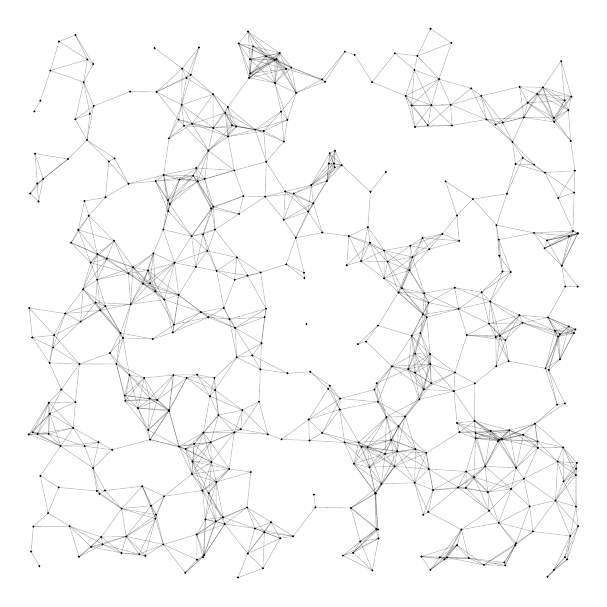
\begin{tikzpicture}[x=0.233333cm, y=0.233333cm]
% Generated by scripts/generate_sirg.py: seed=random, vertices=478, line width=0.2pt, opacity=0.28

% Vertices
\coordinate (v0) at (-1.5881397,12.026207);
\coordinate (v1) at (-0.69744494,12.872793);
\coordinate (v2) at (-3.3106706,5.8769894);
\coordinate (v3) at (6.9236226,10.821382);
\coordinate (v4) at (7.0152767,-10.121379);
\coordinate (v5) at (4.3511735,1.395342);
\coordinate (v6) at (4.9233346,-8.8358072);
\coordinate (v7) at (1.3942447,-4.4503278);
\coordinate (v8) at (9.2680538,-6.3604511);
\coordinate (v9) at (12.720227,-7.825832);
\coordinate (v10) at (0.49744792,5.4779335);
\coordinate (v11) at (8.4491423,-6.9697884);
\coordinate (v12) at (-10.218319,-3.2609045);
\coordinate (v13) at (8.3202605,-6.4754596);
\coordinate (v14) at (5.9987297,12.738388);
\coordinate (v15) at (-9.862112,-1.8496412);
\coordinate (v16) at (5.6675102,-3.5378654);
\coordinate (v17) at (6.0127136,-9.7266833);
\coordinate (v18) at (0.60982498,-11.062435);
\coordinate (v19) at (14.905025,3.8536982);
\coordinate (v20) at (1.2347999,6.6945929);
\coordinate (v21) at (8.4355069,3.4379386);
\coordinate (v22) at (-3.8079325,-6.9935795);
\coordinate (v23) at (-8.4039537,-5.1403075);
\coordinate (v24) at (-12.03375,0.80235802);
\coordinate (v25) at (10.600564,-7.3858162);
\coordinate (v26) at (-9.7710008,-4.9786791);
\coordinate (v27) at (3.465604,4.1813891);
\coordinate (v28) at (12.508131,3.8728528);
\coordinate (v29) at (-14.507989,-7.0628896);
\coordinate (v30) at (7.9748016,10.84076);
\coordinate (v31) at (-7.6693927,4.0507067);
\coordinate (v32) at (6.8622272,-3.2681471);
\coordinate (v33) at (-8.0986136,0.69215848);
\coordinate (v34) at (-4.0772854,-8.9734755);
\coordinate (v35) at (-5.8357212,-13.916116);
\coordinate (v36) at (-7.4125527,5.6548416);
\coordinate (v37) at (-2.2013471,9.4139487);
\coordinate (v38) at (9.6569004,0.63820453);
\coordinate (v39) at (-2.9946679,12.309701);
\coordinate (v40) at (8.3142757,4.8155949);
\coordinate (v41) at (-7.3991529,5.059611);
\coordinate (v42) at (-6.3968019,-4.0206361);
\coordinate (v43) at (3.370075,-2.0453668);
\coordinate (v44) at (7.6991253,6.6760033);
\coordinate (v45) at (6.0338892,-2.6990363);
\coordinate (v46) at (-5.2729677,2.8958156);
\coordinate (v47) at (-13.665283,-2.366372);
\coordinate (v48) at (10.591129,-11.907785);
\coordinate (v49) at (11.160028,-6.8671544);
\coordinate (v50) at (-5.0627927,5.1996547);
\coordinate (v51) at (-8.0956821,-11.681118);
\coordinate (v52) at (-0.009832281,1.69992);
\coordinate (v53) at (6.7685569,0.073401165);
\coordinate (v54) at (-6.0993716,9.8051634);
\coordinate (v55) at (1.3450608,7.641056);
\coordinate (v56) at (12.270119,-11.01672);
\coordinate (v57) at (-7.0874319,-1.1228156);
\coordinate (v58) at (2.7049595,-8.6933045);
\coordinate (v59) at (14.020182,2.0810846);
\coordinate (v60) at (-1.3279982,13.660384);
\coordinate (v61) at (-5.8253843,-3.8466762);
\coordinate (v62) at (-2.9359699,12.550369);
\coordinate (v63) at (14.188864,-13.776163);
\coordinate (v64) at (2.2184441,13.73903);
\coordinate (v65) at (-1.977128,-7.0912687);
\coordinate (v66) at (-1.302172,-12.748319);
\coordinate (v67) at (-2.8217164,-2.7971267);
\coordinate (v68) at (-3.7788285,1.3142058);
\coordinate (v69) at (14.676483,-1.580911);
\coordinate (v70) at (-2.9483787,13.324926);
\coordinate (v71) at (2.6632227,-13.53982);
\coordinate (v72) at (-5.7263722,13.965962);
\coordinate (v73) at (5.7771358,3.1717275);
\coordinate (v74) at (9.8502677,-8.8339674);
\coordinate (v75) at (6.0560775,-7.8975964);
\coordinate (v76) at (-1.5026428,13.331971);
\coordinate (v77) at (-13.218044,-4.6512984);
\coordinate (v78) at (13.613561,9.9091198);
\coordinate (v79) at (14.315986,-13.898867);
\coordinate (v80) at (-6.5412658,9.7063212);
\coordinate (v81) at (14.841125,-8.6482102);
\coordinate (v82) at (14.801507,-8.9550546);
\coordinate (v83) at (6.6733285,-0.7239316);
\coordinate (v84) at (13.677463,-10.700445);
\coordinate (v85) at (-12.449611,14.641819);
\coordinate (v86) at (10.4168,9.7693356);
\coordinate (v87) at (10.061829,-1.070088);
\coordinate (v88) at (5.8914028,2.5556264);
\coordinate (v89) at (14.4136,3.6908828);
\coordinate (v90) at (-7.6449763,7.0267778);
\coordinate (v91) at (-10.82217,-0.11521199);
\coordinate (v92) at (13.247182,-14.842604);
\coordinate (v93) at (-7.316466,5.4392645);
\coordinate (v94) at (14.175329,11.082701);
\coordinate (v95) at (-7.1176355,-3.8670493);
\coordinate (v96) at (11.127301,-3.1047335);
\coordinate (v97) at (-1.1043003,8.8429482);
\coordinate (v98) at (4.7376437,-7.393797);
\coordinate (v99) at (-5.0893959,-7.5236028);
\coordinate (v100) at (10.590331,3.5045379);
\coordinate (v101) at (-4.9399013,5.2981312);
\coordinate (v102) at (-3.5583592,14.177589);
\coordinate (v103) at (14.786581,-9.3120647);
\coordinate (v104) at (6.2668034,-5.188145);
\coordinate (v105) at (10.54898,-7.4676358);
\coordinate (v106) at (7.7709412,-13.793774);
\coordinate (v107) at (6.3243258,-1.588157);
\coordinate (v108) at (-5.9859233,-7.6083152);
\coordinate (v109) at (-8.3887249,1.1276189);
\coordinate (v110) at (5.0612623,-8.0113073);
\coordinate (v111) at (-14.907246,6.0166801);
\coordinate (v112) at (-13.904688,-7.0671265);
\coordinate (v113) at (2.4296654,3.7018531);
\coordinate (v114) at (14.729802,7.2595399);
\coordinate (v115) at (0.010230073,1.4098446);
\coordinate (v116) at (1.3864289,8.208477);
\coordinate (v117) at (13.826703,5.7690315);
\coordinate (v118) at (3.9207262,-12.247633);
\coordinate (v119) at (-2.4543858,-5.3169271);
\coordinate (v120) at (-14.411819,-14.267937);
\coordinate (v121) at (5.7333565,1.8418241);
\coordinate (v122) at (-3.3645841,-5.7734058);
\coordinate (v123) at (-11.488284,-8.9326334);
\coordinate (v124) at (2.7476997,13.563775);
\coordinate (v125) at (2.9245022,-2.183376);
\coordinate (v126) at (11.922725,-7.111884);
\coordinate (v127) at (3.8929602,-10.315018);
\coordinate (v128) at (13.593932,10.13162);
\coordinate (v129) at (-7.9952276,-5.2216211);
\coordinate (v130) at (-11.141472,-10.333869);
\coordinate (v131) at (-4.6660061,-6.0464645);
\coordinate (v132) at (10.457988,-3.3857739);
\coordinate (v133) at (1.6825982,8.3407979);
\coordinate (v134) at (11.726248,11.822729);
\coordinate (v135) at (-13.842925,-5.9713486);
\coordinate (v136) at (14.37753,10.558041);
\coordinate (v137) at (14.505312,8.8754039);
\coordinate (v138) at (12.523839,7.5846594);
\coordinate (v139) at (6.0284425,9.6332376);
\coordinate (v140) at (-8.0584611,-11.467973);
\coordinate (v141) at (-14.358505,11.06989);
\coordinate (v142) at (3.9485783,-4.3091009);
\coordinate (v143) at (-10.741952,2.471263);
\coordinate (v144) at (-10.813835,5.8065384);
\coordinate (v145) at (4.0159066,-5.3231865);
\coordinate (v146) at (10.14651,-6.9022099);
\coordinate (v147) at (-11.045617,-12.683303);
\coordinate (v148) at (6.4792072,-11.471379);
\coordinate (v149) at (5.1326463,0.6318123);
\coordinate (v150) at (0.24474044,-6.2848916);
\coordinate (v151) at (-3.1101058,-11.069764);
\coordinate (v152) at (4.015701,-12.269163);
\coordinate (v153) at (8.9563008,-13.827995);
\coordinate (v154) at (-14.650078,8.1827288);
\coordinate (v155) at (-6.1782626,12.478318);
\coordinate (v156) at (11.492732,-13.128045);
\coordinate (v157) at (6.5337729,0.58857622);
\coordinate (v158) at (-11.2583,2.71724);
\coordinate (v159) at (10.061202,-11.255153);
\coordinate (v160) at (-6.0741406,-8.5716009);
\coordinate (v161) at (11.339581,8.8207692);
\coordinate (v162) at (-13.345532,14.285076);
\coordinate (v163) at (-9.6850401,-12.648564);
\coordinate (v164) at (-11.483941,13.064101);
\coordinate (v165) at (11.263658,-10.065089);
\coordinate (v166) at (11.533805,-13.018606);
\coordinate (v167) at (-11.962424,5.6075771);
\coordinate (v168) at (4.4356638,7.1842006);
\coordinate (v169) at (8.4050311,-0.26439746);
\coordinate (v170) at (-13.259039,-7.7302399);
\coordinate (v171) at (4.4030215,-8.1565647);
\coordinate (v172) at (14.885738,0.94479797);
\coordinate (v173) at (-6.1107766,-9.2532973);
\coordinate (v174) at (3.6071934,6.1124651);
\coordinate (v175) at (1.6587529,7.4419719);
\coordinate (v176) at (-11.626798,2.2546248);
\coordinate (v177) at (-5.2120214,8.34978);
\coordinate (v178) at (-9.047265,-5.6654708);
\coordinate (v179) at (-14.779095,-6.9800996);
\coordinate (v180) at (14.882511,3.8338636);
\coordinate (v181) at (0.28768537,-7.4256068);
\coordinate (v182) at (-8.0871281,6.6879413);
\coordinate (v183) at (11.880805,-1.0203647);
\coordinate (v184) at (-5.7915248,6.6846402);
\coordinate (v185) at (6.1612385,13.504549);
\coordinate (v186) at (6.5166117,-4.6475305);
\coordinate (v187) at (-8.3840242,-7.3798316);
\coordinate (v188) at (6.4610056,-0.56525494);
\coordinate (v189) at (14.634718,3.9777973);
\coordinate (v190) at (0.12451978,-1.0929424);
\coordinate (v191) at (-6.8324729,0.49598553);
\coordinate (v192) at (0.98053448,12.228143);
\coordinate (v193) at (-4.8529055,4.0520199);
\coordinate (v194) at (-8.0324136,11.548464);
\coordinate (v195) at (10.424319,-1.8007475);
\coordinate (v196) at (9.6367058,11.327923);
\coordinate (v197) at (9.7790219,-14.198009);
\coordinate (v198) at (-6.6416669,12.813731);
\coordinate (v199) at (11.715508,-0.60518173);
\coordinate (v200) at (-4.1542125,10.724847);
\coordinate (v201) at (-9.5097159,-3.867135);
\coordinate (v202) at (-6.4495585,-7.885253);
\coordinate (v203) at (14.404953,-1.2187441);
\coordinate (v204) at (-1.0322623,6.1221851);
\coordinate (v205) at (-11.352232,0.076217045);
\coordinate (v206) at (14.795055,-11.027318);
\coordinate (v207) at (-9.9431547,-13.547715);
\coordinate (v208) at (-5.4853102,-7.0015335);
\coordinate (v209) at (-6.8388632,10.039148);
\coordinate (v210) at (-0.97175035,2.1617101);
\coordinate (v211) at (13.26984,-0.73389817);
\coordinate (v212) at (-10.569704,-2.6681259);
\coordinate (v213) at (14.209754,0.95960337);
\coordinate (v214) at (-8.7714594,1.1062391);
\coordinate (v215) at (14.543673,11.288916);
\coordinate (v216) at (3.054317,-12.924522);
\coordinate (v217) at (11.957868,-9.5047332);
\coordinate (v218) at (8.3215097,-13.123273);
\coordinate (v219) at (8.5548669,-12.276829);
\coordinate (v220) at (13.64936,-1.458269);
\coordinate (v221) at (12.56345,-6.5149302);
\coordinate (v222) at (-4.14542,9.1163764);
\coordinate (v223) at (6.8029034,2.9818523);
\coordinate (v224) at (-7.3590171,9.0158317);
\coordinate (v225) at (12.988132,11.791428);
\coordinate (v226) at (6.854872,-2.7212249);
\coordinate (v227) at (4.2013863,-9.791253);
\coordinate (v228) at (-12.168062,-0.95865205);
\coordinate (v229) at (11.03449,6.0032378);
\coordinate (v230) at (5.5242685,11.329941);
\coordinate (v231) at (-14.356852,-9.3498048);
\coordinate (v232) at (-1.8048866,-11.873707);
\coordinate (v233) at (9.0877613,11.736176);
\coordinate (v234) at (-5.8973437,2.0226954);
\coordinate (v235) at (14.089787,-7.8016765);
\coordinate (v236) at (14.689582,6.0653829);
\coordinate (v237) at (-5.4981174,-13.775859);
\coordinate (v238) at (-2.1560221,-0.70983164);
\coordinate (v239) at (13.222461,3.4660049);
\coordinate (v240) at (-4.9499483,9.5795746);
\coordinate (v241) at (6.7295798,9.7337435);
\coordinate (v242) at (-13.365977,-9.981143);
\coordinate (v243) at (3.4458664,-7.7890332);
\coordinate (v244) at (13.098675,7.1530703);
\coordinate (v245) at (-11.265095,1.325368);
\coordinate (v246) at (-9.7360282,-5.2685204);
\coordinate (v247) at (-0.46183673,3.609575);
\coordinate (v248) at (-8.4864631,-6.8531373);
\coordinate (v249) at (-0.56807726,6.0163821);
\coordinate (v250) at (6.032473,-3.7339469);
\coordinate (v251) at (-11.949951,-7.7374475);
\coordinate (v252) at (6.6491118,-8.1050422);
\coordinate (v253) at (-6.8103061,-7.754226);
\coordinate (v254) at (8.1941967,0.8897363);
\coordinate (v255) at (-11.817998,8.9291749);
\coordinate (v256) at (9.1834766,5.7125989);
\coordinate (v257) at (5.1323117,-6.6553844);
\coordinate (v258) at (-8.7084968,-4.0223773);
\coordinate (v259) at (13.798122,-8.5747857);
\coordinate (v260) at (-14.526609,6.5564083);
\coordinate (v261) at (-5.8472399,-12.538798);
\coordinate (v262) at (-9.3148722,2.000105);
\coordinate (v263) at (7.5236853,3.8179614);
\coordinate (v264) at (0.38711777,6.475579);
\coordinate (v265) at (6.8708358,14.981079);
\coordinate (v266) at (-2.7785685,14.029976);
\coordinate (v267) at (7.3838972,-13.783256);
\coordinate (v268) at (-4.8478701,-4.6849515);
\coordinate (v269) at (4.0418579,-12.763586);
\coordinate (v270) at (-0.98446336,12.794926);
\coordinate (v271) at (-7.6227877,-10.461383);
\coordinate (v272) at (-3.675265,-2.8991762);
\coordinate (v273) at (8.3771484,-9.9823756);
\coordinate (v274) at (-4.415003,-11.602718);
\coordinate (v275) at (4.7735538,-3.3897071);
\coordinate (v276) at (-10.343107,3.443136);
\coordinate (v277) at (5.4962176,-6.1164403);
\coordinate (v278) at (10.953099,-1.9683667);
\coordinate (v279) at (11.537958,-8.9188968);
\coordinate (v280) at (-9.9357008,-11.135465);
\coordinate (v281) at (-3.6642829,2.5345153);
\coordinate (v282) at (-10.835822,-10.149429);
\coordinate (v283) at (-4.7818445,-9.6808361);
\coordinate (v284) at (-8.8117173,-9.9173318);
\coordinate (v285) at (-7.6679491,-13.083377);
\coordinate (v286) at (-5.0481287,-8.6080932);
\coordinate (v287) at (-10.319127,7.922894);
\coordinate (v288) at (-8.137952,13.928722);
\coordinate (v289) at (6.7525913,-11.321993);
\coordinate (v290) at (-0.90775285,-3.7693091);
\coordinate (v291) at (-9.5664622,1.66524);
\coordinate (v292) at (-12.256111,-13.754734);
\coordinate (v293) at (8.2079728,-3.7311467);
\coordinate (v294) at (5.854793,-1.7244226);
\coordinate (v295) at (1.9589595,-5.1463266);
\coordinate (v296) at (10.648569,-1.7308252);
\coordinate (v297) at (-2.6686262,9.492354);
\coordinate (v298) at (-5.1929492,-10.293098);
\coordinate (v299) at (-6.6672512,10.835109);
\coordinate (v300) at (4.0095142,-1.1748867);
\coordinate (v301) at (9.2376173,-9.4144561);
\coordinate (v302) at (-12.450592,-5.3371789);
\coordinate (v303) at (-4.3727686,-0.21670753);
\coordinate (v304) at (-5.2238342,-0.71638382);
\coordinate (v305) at (-4.7639026,1.8064173);
\coordinate (v306) at (1.6233725,7.6548976);
\coordinate (v307) at (2.5493382,-11.098581);
\coordinate (v308) at (-5.5411435,-10.152434);
\coordinate (v309) at (10.615576,2.6249292);
\coordinate (v310) at (-10.450585,-7.9330456);
\coordinate (v311) at (10.12478,0.13777616);
\coordinate (v312) at (6.9125589,-4.3105458);
\coordinate (v313) at (3.6997779,12.078741);
\coordinate (v314) at (-6.0419532,6.9834352);
\coordinate (v315) at (-12.23316,-3.2656505);
\coordinate (v316) at (0.97942562,-7.0140727);
\coordinate (v317) at (8.8526069,-1.6865049);
\coordinate (v318) at (12.707202,-7.4772613);
\coordinate (v319) at (8.0434079,9.720355);
\coordinate (v320) at (-11.456832,10.7819);
\coordinate (v321) at (-9.4454052,-0.013111992);
\coordinate (v322) at (13.916672,-1.6402493);
\coordinate (v323) at (-10.971219,-13.088083);
\coordinate (v324) at (-4.8109851,-11.824734);
\coordinate (v325) at (-12.682991,3.3380658);
\coordinate (v326) at (12.164231,10.955719);
\coordinate (v327) at (3.1173435,-7.7692935);
\coordinate (v328) at (-1.6020144,13.299739);
\coordinate (v329) at (11.501503,7.6172149);
\coordinate (v330) at (2.2013029,-7.5329973);
\coordinate (v331) at (-12.852659,7.8946613);
\coordinate (v332) at (13.308571,-3.5884258);
\coordinate (v333) at (-5.3747493,-11.722563);
\coordinate (v334) at (9.2906918,-4.3205289);
\coordinate (v335) at (10.759695,-7.3559204);
\coordinate (v336) at (14.760208,-1.3819077);
\coordinate (v337) at (5.321218,0.86274055);
\coordinate (v338) at (3.824395,-4.6569384);
\coordinate (v339) at (-0.60848458,-12.639732);
\coordinate (v340) at (-14.964328,-0.22034356);
\coordinate (v341) at (11.954331,10.153296);
\coordinate (v342) at (-2.679,-12.215176);
\coordinate (v343) at (-7.3544833,-5.7688109);
\coordinate (v344) at (-7.0577344,2.2425093);
\coordinate (v345) at (1.9336397,-5.7427892);
\coordinate (v346) at (-14.860238,-13.472884);
\coordinate (v347) at (13.087244,3.0358437);
\coordinate (v348) at (11.243733,1.7405313);
\coordinate (v349) at (-13.006702,-0.51645073);
\coordinate (v350) at (-2.0644052,7.7441444);
\coordinate (v351) at (-8.9741958,-13.616221);
\coordinate (v352) at (8.0119806,14.214233);
\coordinate (v353) at (3.5812601,3.3330144);
\coordinate (v354) at (-0.91442833,10.027806);
\coordinate (v355) at (3.5566418,-8.8811019);
\coordinate (v356) at (6.7792243,-8.9786726);
\coordinate (v357) at (-5.1242264,-5.018113);
\coordinate (v358) at (-8.2452723,-1.9034152);
\coordinate (v359) at (-14.460085,5.5752498);
\coordinate (v360) at (1.3077169,-4.6167789);
\coordinate (v361) at (14.192394,-5.4082192);
\coordinate (v362) at (-3.7576668,-1.3026089);
\coordinate (v363) at (12.445015,-12.378571);
\coordinate (v364) at (-2.3231421,-2.1330371);
\coordinate (v365) at (-11.195541,-7.5219059);
\coordinate (v366) at (9.3309858,-7.0213331);
\coordinate (v367) at (10.466366,4.290356);
\coordinate (v368) at (10.792058,1.7678686);
\coordinate (v369) at (-8.3389062,-10.97879);
\coordinate (v370) at (-3.450908,-6.8186186);
\coordinate (v371) at (-12.7641,-12.092923);
\coordinate (v372) at (-2.3687007,1.718615);
\coordinate (v373) at (-10.635938,7.7627137);
\coordinate (v374) at (-9.9995,-1.579464);
\coordinate (v375) at (-11.998411,12.073712);
\coordinate (v376) at (13.770761,-5.4742888);
\coordinate (v377) at (-12.293032,4.0385463);
\coordinate (v378) at (-6.7870391,6.7710088);
\coordinate (v379) at (-13.815976,12.705653);
\coordinate (v380) at (-1.2329955,-7.364842);
\coordinate (v381) at (-6.1277055,3.689481);
\coordinate (v382) at (-9.562317,6.5504952);
\coordinate (v383) at (7.3397434,12.24348);
\coordinate (v384) at (6.3807726,-13.75135);
\coordinate (v385) at (1.1329348,12.10284);
\coordinate (v386) at (-13.609187,-1.6973366);
\coordinate (v387) at (-2.0808332,13.486342);
\coordinate (v388) at (-3.0835666,1.5520933);
\coordinate (v389) at (4.3518488,2.9127426);
\coordinate (v390) at (2.1153017,-13.691914);
\coordinate (v391) at (-3.6053937,-14.886291);
\coordinate (v392) at (10.894631,-14.06432);
\coordinate (v393) at (3.8584735,-10.295258);
\coordinate (v394) at (-13.858538,-3.2041002);
\coordinate (v395) at (-2.9029796,-9.1437518);
\coordinate (v396) at (0.33012357,-3.688449);
\coordinate (v397) at (4.5389196,2.3076644);
\coordinate (v398) at (-14.797737,-1.8244197);
\coordinate (v399) at (-7.6120419,0.23904738);
\coordinate (v400) at (9.9965919,-10.233233);
\coordinate (v401) at (-14.680933,10.484644);
\coordinate (v402) at (-13.937844,-11.375263);
\coordinate (v403) at (9.9160545,10.0445);
\coordinate (v404) at (3.0944547,2.3348628);
\coordinate (v405) at (-5.8718895,7.4018941);
\coordinate (v406) at (-5.6259657,-0.43923183);
\coordinate (v407) at (-12.571114,-6.7405883);
\coordinate (v408) at (10.940817,-14.22702);
\coordinate (v409) at (-8.2056759,2.7548339);
\coordinate (v410) at (-6.4704749,-14.624833);
\coordinate (v411) at (13.133775,-3.5016662);
\coordinate (v412) at (-4.071018,-0.82582022);
\coordinate (v413) at (8.8153509,-9.1157696);
\coordinate (v414) at (-12.456936,10.053165);
\coordinate (v415) at (5.8405277,10.803675);
\coordinate (v416) at (-4.885475,-4.0225949);
\coordinate (v417) at (-11.282365,-10.173362);
\coordinate (v418) at (-2.0752548,-0.25363794);
\coordinate (v419) at (0.21638715,5.0339842);
\coordinate (v420) at (-3.8012911,7.2701545);
\coordinate (v421) at (-2.126734,5.844044);
\coordinate (v422) at (-3.9224477,9.7317894);
\coordinate (v423) at (6.8680173,-14.46372);
\coordinate (v424) at (-6.4098417,12.301486);
\coordinate (v425) at (-2.2437097,-14.384966);
\coordinate (v426) at (-3.547302,4.905493);
\coordinate (v427) at (-3.0716579,-13.579667);
\coordinate (v428) at (4.9346983,13.647844);
\coordinate (v429) at (14.114888,-9.6516762);
\coordinate (v430) at (-4.3227314,-11.975967);
\coordinate (v431) at (-5.501816,3.7963782);
\coordinate (v432) at (8.1511476,-4.7386175);
\coordinate (v433) at (-8.6498262,-13.700989);
\coordinate (v434) at (-9.4778241,11.559051);
\coordinate (v435) at (10.805845,9.8784298);
\coordinate (v436) at (-7.1503697,-1.5427427);
\coordinate (v437) at (8.8014393,-10.005694);
\coordinate (v438) at (-3.6971286,9.6597985);
\coordinate (v439) at (0.98510182,3.8892433);
\coordinate (v440) at (-8.4961578,1.8299487);
\coordinate (v441) at (-5.4110936,6.8126553);
\coordinate (v442) at (13.9904,13.222258);
\coordinate (v443) at (13.818716,-1.7690872);
\coordinate (v444) at (-11.098666,-0.34531364);
\coordinate (v445) at (13.922784,-3.0048643);
\coordinate (v446) at (-2.1652604,-12.427217);
\coordinate (v447) at (9.3310277,-7.3095353);
\coordinate (v448) at (2.9609889,-7.5314318);
\coordinate (v449) at (-7.3590301,-5.8263705);
\coordinate (v450) at (-0.43580425,11.493644);
\coordinate (v451) at (-1.1142952,4.5908674);
\coordinate (v452) at (2.0432364,7.5572308);
\coordinate (v453) at (-2.3856855,-3.5518494);
\coordinate (v454) at (-11.801522,13.310029);
\coordinate (v455) at (-14.989576,-7.1003997);
\coordinate (v456) at (6.4397367,3.5985291);
\coordinate (v457) at (14.908147,-12.091807);
\coordinate (v458) at (-11.598407,-13.214382);
\coordinate (v459) at (-5.4388257,-13.65548);
\coordinate (v460) at (3.7117467,-14.502492);
\coordinate (v461) at (-1.2555754,10.473759);
\coordinate (v462) at (-4.2952912,10.405191);
\coordinate (v463) at (-11.663642,10.343268);
\coordinate (v464) at (0.52265757,-10.373864);
\coordinate (v465) at (-4.9573463,11.418258);
\coordinate (v466) at (13.59269,-14.470099);
\coordinate (v467) at (14.479266,-12.625779);
\coordinate (v468) at (-14.206017,6.8081753);
\coordinate (v469) at (12.686042,11.432026);
\coordinate (v470) at (-14.740083,-12.110676);
\coordinate (v471) at (11.894154,7.9551317);
\coordinate (v472) at (-13.903671,-5.3715553);
\coordinate (v473) at (-11.722258,4.806458);
\coordinate (v474) at (7.6325141,-13.89669);
\coordinate (v475) at (4.4730507,-6.1529328);
\coordinate (v476) at (-3.0565386,14.831829);
\coordinate (v477) at (2.3203553,2.1103179);

% Edges
\draw[line width=0.2pt, opacity=0.28] (v0) -- (v1);
\draw[line width=0.2pt, opacity=0.28] (v0) -- (v39);
\draw[line width=0.2pt, opacity=0.28] (v0) -- (v60);
\draw[line width=0.2pt, opacity=0.28] (v0) -- (v62);
\draw[line width=0.2pt, opacity=0.28] (v0) -- (v70);
\draw[line width=0.2pt, opacity=0.28] (v0) -- (v76);
\draw[line width=0.2pt, opacity=0.28] (v0) -- (v270);
\draw[line width=0.2pt, opacity=0.28] (v0) -- (v328);
\draw[line width=0.2pt, opacity=0.28] (v0) -- (v354);
\draw[line width=0.2pt, opacity=0.28] (v0) -- (v387);
\draw[line width=0.2pt, opacity=0.28] (v0) -- (v450);
\draw[line width=0.2pt, opacity=0.28] (v0) -- (v461);
\draw[line width=0.2pt, opacity=0.28] (v1) -- (v60);
\draw[line width=0.2pt, opacity=0.28] (v1) -- (v76);
\draw[line width=0.2pt, opacity=0.28] (v1) -- (v192);
\draw[line width=0.2pt, opacity=0.28] (v1) -- (v270);
\draw[line width=0.2pt, opacity=0.28] (v1) -- (v328);
\draw[line width=0.2pt, opacity=0.28] (v1) -- (v385);
\draw[line width=0.2pt, opacity=0.28] (v1) -- (v387);
\draw[line width=0.2pt, opacity=0.28] (v1) -- (v450);
\draw[line width=0.2pt, opacity=0.28] (v2) -- (v50);
\draw[line width=0.2pt, opacity=0.28] (v2) -- (v101);
\draw[line width=0.2pt, opacity=0.28] (v2) -- (v420);
\draw[line width=0.2pt, opacity=0.28] (v2) -- (v421);
\draw[line width=0.2pt, opacity=0.28] (v2) -- (v426);
\draw[line width=0.2pt, opacity=0.28] (v3) -- (v14);
\draw[line width=0.2pt, opacity=0.28] (v3) -- (v30);
\draw[line width=0.2pt, opacity=0.28] (v3) -- (v139);
\draw[line width=0.2pt, opacity=0.28] (v3) -- (v230);
\draw[line width=0.2pt, opacity=0.28] (v3) -- (v241);
\draw[line width=0.2pt, opacity=0.28] (v3) -- (v319);
\draw[line width=0.2pt, opacity=0.28] (v3) -- (v383);
\draw[line width=0.2pt, opacity=0.28] (v3) -- (v415);
\draw[line width=0.2pt, opacity=0.28] (v4) -- (v17);
\draw[line width=0.2pt, opacity=0.28] (v4) -- (v148);
\draw[line width=0.2pt, opacity=0.28] (v4) -- (v252);
\draw[line width=0.2pt, opacity=0.28] (v4) -- (v273);
\draw[line width=0.2pt, opacity=0.28] (v4) -- (v289);
\draw[line width=0.2pt, opacity=0.28] (v4) -- (v356);
\draw[line width=0.2pt, opacity=0.28] (v4) -- (v413);
\draw[line width=0.2pt, opacity=0.28] (v4) -- (v437);
\draw[line width=0.2pt, opacity=0.28] (v5) -- (v88);
\draw[line width=0.2pt, opacity=0.28] (v5) -- (v121);
\draw[line width=0.2pt, opacity=0.28] (v5) -- (v149);
\draw[line width=0.2pt, opacity=0.28] (v5) -- (v337);
\draw[line width=0.2pt, opacity=0.28] (v5) -- (v353);
\draw[line width=0.2pt, opacity=0.28] (v5) -- (v389);
\draw[line width=0.2pt, opacity=0.28] (v5) -- (v397);
\draw[line width=0.2pt, opacity=0.28] (v5) -- (v404);
\draw[line width=0.2pt, opacity=0.28] (v6) -- (v17);
\draw[line width=0.2pt, opacity=0.28] (v6) -- (v75);
\draw[line width=0.2pt, opacity=0.28] (v6) -- (v98);
\draw[line width=0.2pt, opacity=0.28] (v6) -- (v110);
\draw[line width=0.2pt, opacity=0.28] (v6) -- (v127);
\draw[line width=0.2pt, opacity=0.28] (v6) -- (v171);
\draw[line width=0.2pt, opacity=0.28] (v6) -- (v227);
\draw[line width=0.2pt, opacity=0.28] (v6) -- (v243);
\draw[line width=0.2pt, opacity=0.28] (v6) -- (v252);
\draw[line width=0.2pt, opacity=0.28] (v6) -- (v327);
\draw[line width=0.2pt, opacity=0.28] (v6) -- (v355);
\draw[line width=0.2pt, opacity=0.28] (v6) -- (v356);
\draw[line width=0.2pt, opacity=0.28] (v6) -- (v393);
\draw[line width=0.2pt, opacity=0.28] (v7) -- (v295);
\draw[line width=0.2pt, opacity=0.28] (v7) -- (v345);
\draw[line width=0.2pt, opacity=0.28] (v7) -- (v360);
\draw[line width=0.2pt, opacity=0.28] (v7) -- (v396);
\draw[line width=0.2pt, opacity=0.28] (v8) -- (v11);
\draw[line width=0.2pt, opacity=0.28] (v8) -- (v13);
\draw[line width=0.2pt, opacity=0.28] (v8) -- (v25);
\draw[line width=0.2pt, opacity=0.28] (v8) -- (v49);
\draw[line width=0.2pt, opacity=0.28] (v8) -- (v105);
\draw[line width=0.2pt, opacity=0.28] (v8) -- (v146);
\draw[line width=0.2pt, opacity=0.28] (v8) -- (v334);
\draw[line width=0.2pt, opacity=0.28] (v8) -- (v335);
\draw[line width=0.2pt, opacity=0.28] (v8) -- (v366);
\draw[line width=0.2pt, opacity=0.28] (v8) -- (v432);
\draw[line width=0.2pt, opacity=0.28] (v8) -- (v447);
\draw[line width=0.2pt, opacity=0.28] (v9) -- (v49);
\draw[line width=0.2pt, opacity=0.28] (v9) -- (v126);
\draw[line width=0.2pt, opacity=0.28] (v9) -- (v217);
\draw[line width=0.2pt, opacity=0.28] (v9) -- (v221);
\draw[line width=0.2pt, opacity=0.28] (v9) -- (v235);
\draw[line width=0.2pt, opacity=0.28] (v9) -- (v259);
\draw[line width=0.2pt, opacity=0.28] (v9) -- (v279);
\draw[line width=0.2pt, opacity=0.28] (v9) -- (v318);
\draw[line width=0.2pt, opacity=0.28] (v9) -- (v335);
\draw[line width=0.2pt, opacity=0.28] (v10) -- (v20);
\draw[line width=0.2pt, opacity=0.28] (v10) -- (v204);
\draw[line width=0.2pt, opacity=0.28] (v10) -- (v247);
\draw[line width=0.2pt, opacity=0.28] (v10) -- (v249);
\draw[line width=0.2pt, opacity=0.28] (v10) -- (v264);
\draw[line width=0.2pt, opacity=0.28] (v10) -- (v419);
\draw[line width=0.2pt, opacity=0.28] (v10) -- (v439);
\draw[line width=0.2pt, opacity=0.28] (v10) -- (v451);
\draw[line width=0.2pt, opacity=0.28] (v11) -- (v13);
\draw[line width=0.2pt, opacity=0.28] (v11) -- (v146);
\draw[line width=0.2pt, opacity=0.28] (v11) -- (v252);
\draw[line width=0.2pt, opacity=0.28] (v11) -- (v366);
\draw[line width=0.2pt, opacity=0.28] (v11) -- (v447);
\draw[line width=0.2pt, opacity=0.28] (v12) -- (v15);
\draw[line width=0.2pt, opacity=0.28] (v12) -- (v26);
\draw[line width=0.2pt, opacity=0.28] (v12) -- (v201);
\draw[line width=0.2pt, opacity=0.28] (v12) -- (v212);
\draw[line width=0.2pt, opacity=0.28] (v12) -- (v246);
\draw[line width=0.2pt, opacity=0.28] (v12) -- (v258);
\draw[line width=0.2pt, opacity=0.28] (v12) -- (v315);
\draw[line width=0.2pt, opacity=0.28] (v12) -- (v374);
\draw[line width=0.2pt, opacity=0.28] (v13) -- (v146);
\draw[line width=0.2pt, opacity=0.28] (v13) -- (v366);
\draw[line width=0.2pt, opacity=0.28] (v13) -- (v432);
\draw[line width=0.2pt, opacity=0.28] (v13) -- (v447);
\draw[line width=0.2pt, opacity=0.28] (v14) -- (v185);
\draw[line width=0.2pt, opacity=0.28] (v14) -- (v230);
\draw[line width=0.2pt, opacity=0.28] (v14) -- (v383);
\draw[line width=0.2pt, opacity=0.28] (v14) -- (v415);
\draw[line width=0.2pt, opacity=0.28] (v14) -- (v428);
\draw[line width=0.2pt, opacity=0.28] (v15) -- (v91);
\draw[line width=0.2pt, opacity=0.28] (v15) -- (v201);
\draw[line width=0.2pt, opacity=0.28] (v15) -- (v212);
\draw[line width=0.2pt, opacity=0.28] (v15) -- (v321);
\draw[line width=0.2pt, opacity=0.28] (v15) -- (v358);
\draw[line width=0.2pt, opacity=0.28] (v15) -- (v374);
\draw[line width=0.2pt, opacity=0.28] (v15) -- (v444);
\draw[line width=0.2pt, opacity=0.28] (v16) -- (v32);
\draw[line width=0.2pt, opacity=0.28] (v16) -- (v45);
\draw[line width=0.2pt, opacity=0.28] (v16) -- (v104);
\draw[line width=0.2pt, opacity=0.28] (v16) -- (v107);
\draw[line width=0.2pt, opacity=0.28] (v16) -- (v142);
\draw[line width=0.2pt, opacity=0.28] (v16) -- (v186);
\draw[line width=0.2pt, opacity=0.28] (v16) -- (v226);
\draw[line width=0.2pt, opacity=0.28] (v16) -- (v250);
\draw[line width=0.2pt, opacity=0.28] (v16) -- (v275);
\draw[line width=0.2pt, opacity=0.28] (v16) -- (v294);
\draw[line width=0.2pt, opacity=0.28] (v16) -- (v312);
\draw[line width=0.2pt, opacity=0.28] (v17) -- (v75);
\draw[line width=0.2pt, opacity=0.28] (v17) -- (v110);
\draw[line width=0.2pt, opacity=0.28] (v17) -- (v148);
\draw[line width=0.2pt, opacity=0.28] (v17) -- (v227);
\draw[line width=0.2pt, opacity=0.28] (v17) -- (v252);
\draw[line width=0.2pt, opacity=0.28] (v17) -- (v289);
\draw[line width=0.2pt, opacity=0.28] (v17) -- (v356);
\draw[line width=0.2pt, opacity=0.28] (v18) -- (v307);
\draw[line width=0.2pt, opacity=0.28] (v18) -- (v339);
\draw[line width=0.2pt, opacity=0.28] (v18) -- (v464);
\draw[line width=0.2pt, opacity=0.28] (v19) -- (v59);
\draw[line width=0.2pt, opacity=0.28] (v19) -- (v89);
\draw[line width=0.2pt, opacity=0.28] (v19) -- (v180);
\draw[line width=0.2pt, opacity=0.28] (v19) -- (v189);
\draw[line width=0.2pt, opacity=0.28] (v19) -- (v239);
\draw[line width=0.2pt, opacity=0.28] (v19) -- (v347);
\draw[line width=0.2pt, opacity=0.28] (v20) -- (v55);
\draw[line width=0.2pt, opacity=0.28] (v20) -- (v116);
\draw[line width=0.2pt, opacity=0.28] (v20) -- (v133);
\draw[line width=0.2pt, opacity=0.28] (v20) -- (v175);
\draw[line width=0.2pt, opacity=0.28] (v20) -- (v249);
\draw[line width=0.2pt, opacity=0.28] (v20) -- (v264);
\draw[line width=0.2pt, opacity=0.28] (v20) -- (v306);
\draw[line width=0.2pt, opacity=0.28] (v20) -- (v419);
\draw[line width=0.2pt, opacity=0.28] (v20) -- (v452);
\draw[line width=0.2pt, opacity=0.28] (v21) -- (v40);
\draw[line width=0.2pt, opacity=0.28] (v21) -- (v223);
\draw[line width=0.2pt, opacity=0.28] (v21) -- (v263);
\draw[line width=0.2pt, opacity=0.28] (v21) -- (v456);
\draw[line width=0.2pt, opacity=0.28] (v22) -- (v34);
\draw[line width=0.2pt, opacity=0.28] (v22) -- (v65);
\draw[line width=0.2pt, opacity=0.28] (v22) -- (v99);
\draw[line width=0.2pt, opacity=0.28] (v22) -- (v122);
\draw[line width=0.2pt, opacity=0.28] (v22) -- (v131);
\draw[line width=0.2pt, opacity=0.28] (v22) -- (v208);
\draw[line width=0.2pt, opacity=0.28] (v22) -- (v286);
\draw[line width=0.2pt, opacity=0.28] (v22) -- (v370);
\draw[line width=0.2pt, opacity=0.28] (v23) -- (v26);
\draw[line width=0.2pt, opacity=0.28] (v23) -- (v95);
\draw[line width=0.2pt, opacity=0.28] (v23) -- (v129);
\draw[line width=0.2pt, opacity=0.28] (v23) -- (v178);
\draw[line width=0.2pt, opacity=0.28] (v23) -- (v201);
\draw[line width=0.2pt, opacity=0.28] (v23) -- (v246);
\draw[line width=0.2pt, opacity=0.28] (v23) -- (v248);
\draw[line width=0.2pt, opacity=0.28] (v23) -- (v258);
\draw[line width=0.2pt, opacity=0.28] (v23) -- (v343);
\draw[line width=0.2pt, opacity=0.28] (v23) -- (v449);
\draw[line width=0.2pt, opacity=0.28] (v24) -- (v91);
\draw[line width=0.2pt, opacity=0.28] (v24) -- (v143);
\draw[line width=0.2pt, opacity=0.28] (v24) -- (v158);
\draw[line width=0.2pt, opacity=0.28] (v24) -- (v176);
\draw[line width=0.2pt, opacity=0.28] (v24) -- (v205);
\draw[line width=0.2pt, opacity=0.28] (v24) -- (v228);
\draw[line width=0.2pt, opacity=0.28] (v24) -- (v245);
\draw[line width=0.2pt, opacity=0.28] (v24) -- (v349);
\draw[line width=0.2pt, opacity=0.28] (v24) -- (v444);
\draw[line width=0.2pt, opacity=0.28] (v25) -- (v49);
\draw[line width=0.2pt, opacity=0.28] (v25) -- (v74);
\draw[line width=0.2pt, opacity=0.28] (v25) -- (v105);
\draw[line width=0.2pt, opacity=0.28] (v25) -- (v126);
\draw[line width=0.2pt, opacity=0.28] (v25) -- (v146);
\draw[line width=0.2pt, opacity=0.28] (v25) -- (v221);
\draw[line width=0.2pt, opacity=0.28] (v25) -- (v279);
\draw[line width=0.2pt, opacity=0.28] (v25) -- (v318);
\draw[line width=0.2pt, opacity=0.28] (v25) -- (v335);
\draw[line width=0.2pt, opacity=0.28] (v25) -- (v366);
\draw[line width=0.2pt, opacity=0.28] (v25) -- (v447);
\draw[line width=0.2pt, opacity=0.28] (v26) -- (v129);
\draw[line width=0.2pt, opacity=0.28] (v26) -- (v178);
\draw[line width=0.2pt, opacity=0.28] (v26) -- (v201);
\draw[line width=0.2pt, opacity=0.28] (v26) -- (v246);
\draw[line width=0.2pt, opacity=0.28] (v26) -- (v258);
\draw[line width=0.2pt, opacity=0.28] (v27) -- (v113);
\draw[line width=0.2pt, opacity=0.28] (v27) -- (v174);
\draw[line width=0.2pt, opacity=0.28] (v27) -- (v353);
\draw[line width=0.2pt, opacity=0.28] (v27) -- (v389);
\draw[line width=0.2pt, opacity=0.28] (v27) -- (v404);
\draw[line width=0.2pt, opacity=0.28] (v28) -- (v89);
\draw[line width=0.2pt, opacity=0.28] (v28) -- (v100);
\draw[line width=0.2pt, opacity=0.28] (v28) -- (v189);
\draw[line width=0.2pt, opacity=0.28] (v28) -- (v239);
\draw[line width=0.2pt, opacity=0.28] (v28) -- (v347);
\draw[line width=0.2pt, opacity=0.28] (v28) -- (v367);
\draw[line width=0.2pt, opacity=0.28] (v29) -- (v112);
\draw[line width=0.2pt, opacity=0.28] (v29) -- (v135);
\draw[line width=0.2pt, opacity=0.28] (v29) -- (v170);
\draw[line width=0.2pt, opacity=0.28] (v29) -- (v179);
\draw[line width=0.2pt, opacity=0.28] (v29) -- (v407);
\draw[line width=0.2pt, opacity=0.28] (v29) -- (v455);
\draw[line width=0.2pt, opacity=0.28] (v29) -- (v472);
\draw[line width=0.2pt, opacity=0.28] (v30) -- (v196);
\draw[line width=0.2pt, opacity=0.28] (v30) -- (v233);
\draw[line width=0.2pt, opacity=0.28] (v30) -- (v241);
\draw[line width=0.2pt, opacity=0.28] (v30) -- (v319);
\draw[line width=0.2pt, opacity=0.28] (v30) -- (v383);
\draw[line width=0.2pt, opacity=0.28] (v30) -- (v403);
\draw[line width=0.2pt, opacity=0.28] (v30) -- (v415);
\draw[line width=0.2pt, opacity=0.28] (v31) -- (v36);
\draw[line width=0.2pt, opacity=0.28] (v31) -- (v41);
\draw[line width=0.2pt, opacity=0.28] (v31) -- (v93);
\draw[line width=0.2pt, opacity=0.28] (v31) -- (v344);
\draw[line width=0.2pt, opacity=0.28] (v31) -- (v381);
\draw[line width=0.2pt, opacity=0.28] (v31) -- (v409);
\draw[line width=0.2pt, opacity=0.28] (v32) -- (v45);
\draw[line width=0.2pt, opacity=0.28] (v32) -- (v104);
\draw[line width=0.2pt, opacity=0.28] (v32) -- (v107);
\draw[line width=0.2pt, opacity=0.28] (v32) -- (v186);
\draw[line width=0.2pt, opacity=0.28] (v32) -- (v226);
\draw[line width=0.2pt, opacity=0.28] (v32) -- (v250);
\draw[line width=0.2pt, opacity=0.28] (v32) -- (v275);
\draw[line width=0.2pt, opacity=0.28] (v32) -- (v293);
\draw[line width=0.2pt, opacity=0.28] (v32) -- (v294);
\draw[line width=0.2pt, opacity=0.28] (v32) -- (v312);
\draw[line width=0.2pt, opacity=0.28] (v32) -- (v432);
\draw[line width=0.2pt, opacity=0.28] (v33) -- (v57);
\draw[line width=0.2pt, opacity=0.28] (v33) -- (v109);
\draw[line width=0.2pt, opacity=0.28] (v33) -- (v191);
\draw[line width=0.2pt, opacity=0.28] (v33) -- (v214);
\draw[line width=0.2pt, opacity=0.28] (v33) -- (v262);
\draw[line width=0.2pt, opacity=0.28] (v33) -- (v291);
\draw[line width=0.2pt, opacity=0.28] (v33) -- (v321);
\draw[line width=0.2pt, opacity=0.28] (v33) -- (v344);
\draw[line width=0.2pt, opacity=0.28] (v33) -- (v399);
\draw[line width=0.2pt, opacity=0.28] (v33) -- (v409);
\draw[line width=0.2pt, opacity=0.28] (v33) -- (v440);
\draw[line width=0.2pt, opacity=0.28] (v34) -- (v99);
\draw[line width=0.2pt, opacity=0.28] (v34) -- (v160);
\draw[line width=0.2pt, opacity=0.28] (v34) -- (v173);
\draw[line width=0.2pt, opacity=0.28] (v34) -- (v283);
\draw[line width=0.2pt, opacity=0.28] (v34) -- (v286);
\draw[line width=0.2pt, opacity=0.28] (v34) -- (v298);
\draw[line width=0.2pt, opacity=0.28] (v34) -- (v308);
\draw[line width=0.2pt, opacity=0.28] (v34) -- (v395);
\draw[line width=0.2pt, opacity=0.28] (v35) -- (v237);
\draw[line width=0.2pt, opacity=0.28] (v35) -- (v261);
\draw[line width=0.2pt, opacity=0.28] (v35) -- (v285);
\draw[line width=0.2pt, opacity=0.28] (v35) -- (v410);
\draw[line width=0.2pt, opacity=0.28] (v35) -- (v459);
\draw[line width=0.2pt, opacity=0.28] (v36) -- (v41);
\draw[line width=0.2pt, opacity=0.28] (v36) -- (v90);
\draw[line width=0.2pt, opacity=0.28] (v36) -- (v93);
\draw[line width=0.2pt, opacity=0.28] (v36) -- (v182);
\draw[line width=0.2pt, opacity=0.28] (v36) -- (v184);
\draw[line width=0.2pt, opacity=0.28] (v36) -- (v314);
\draw[line width=0.2pt, opacity=0.28] (v36) -- (v378);
\draw[line width=0.2pt, opacity=0.28] (v37) -- (v97);
\draw[line width=0.2pt, opacity=0.28] (v37) -- (v222);
\draw[line width=0.2pt, opacity=0.28] (v37) -- (v297);
\draw[line width=0.2pt, opacity=0.28] (v37) -- (v350);
\draw[line width=0.2pt, opacity=0.28] (v37) -- (v354);
\draw[line width=0.2pt, opacity=0.28] (v37) -- (v422);
\draw[line width=0.2pt, opacity=0.28] (v37) -- (v438);
\draw[line width=0.2pt, opacity=0.28] (v37) -- (v461);
\draw[line width=0.2pt, opacity=0.28] (v38) -- (v87);
\draw[line width=0.2pt, opacity=0.28] (v38) -- (v169);
\draw[line width=0.2pt, opacity=0.28] (v38) -- (v254);
\draw[line width=0.2pt, opacity=0.28] (v38) -- (v311);
\draw[line width=0.2pt, opacity=0.28] (v38) -- (v348);
\draw[line width=0.2pt, opacity=0.28] (v38) -- (v368);
\draw[line width=0.2pt, opacity=0.28] (v39) -- (v60);
\draw[line width=0.2pt, opacity=0.28] (v39) -- (v62);
\draw[line width=0.2pt, opacity=0.28] (v39) -- (v70);
\draw[line width=0.2pt, opacity=0.28] (v39) -- (v76);
\draw[line width=0.2pt, opacity=0.28] (v39) -- (v102);
\draw[line width=0.2pt, opacity=0.28] (v39) -- (v200);
\draw[line width=0.2pt, opacity=0.28] (v39) -- (v266);
\draw[line width=0.2pt, opacity=0.28] (v39) -- (v270);
\draw[line width=0.2pt, opacity=0.28] (v39) -- (v328);
\draw[line width=0.2pt, opacity=0.28] (v39) -- (v387);
\draw[line width=0.2pt, opacity=0.28] (v40) -- (v44);
\draw[line width=0.2pt, opacity=0.28] (v40) -- (v256);
\draw[line width=0.2pt, opacity=0.28] (v40) -- (v263);
\draw[line width=0.2pt, opacity=0.28] (v41) -- (v90);
\draw[line width=0.2pt, opacity=0.28] (v41) -- (v93);
\draw[line width=0.2pt, opacity=0.28] (v41) -- (v182);
\draw[line width=0.2pt, opacity=0.28] (v41) -- (v378);
\draw[line width=0.2pt, opacity=0.28] (v41) -- (v381);
\draw[line width=0.2pt, opacity=0.28] (v42) -- (v61);
\draw[line width=0.2pt, opacity=0.28] (v42) -- (v95);
\draw[line width=0.2pt, opacity=0.28] (v42) -- (v129);
\draw[line width=0.2pt, opacity=0.28] (v42) -- (v268);
\draw[line width=0.2pt, opacity=0.28] (v42) -- (v343);
\draw[line width=0.2pt, opacity=0.28] (v42) -- (v357);
\draw[line width=0.2pt, opacity=0.28] (v42) -- (v416);
\draw[line width=0.2pt, opacity=0.28] (v42) -- (v449);
\draw[line width=0.2pt, opacity=0.28] (v43) -- (v125);
\draw[line width=0.2pt, opacity=0.28] (v43) -- (v275);
\draw[line width=0.2pt, opacity=0.28] (v43) -- (v300);
\draw[line width=0.2pt, opacity=0.28] (v44) -- (v256);
\draw[line width=0.2pt, opacity=0.28] (v45) -- (v83);
\draw[line width=0.2pt, opacity=0.28] (v45) -- (v107);
\draw[line width=0.2pt, opacity=0.28] (v45) -- (v186);
\draw[line width=0.2pt, opacity=0.28] (v45) -- (v226);
\draw[line width=0.2pt, opacity=0.28] (v45) -- (v250);
\draw[line width=0.2pt, opacity=0.28] (v45) -- (v275);
\draw[line width=0.2pt, opacity=0.28] (v45) -- (v294);
\draw[line width=0.2pt, opacity=0.28] (v45) -- (v312);
\draw[line width=0.2pt, opacity=0.28] (v46) -- (v193);
\draw[line width=0.2pt, opacity=0.28] (v46) -- (v234);
\draw[line width=0.2pt, opacity=0.28] (v46) -- (v281);
\draw[line width=0.2pt, opacity=0.28] (v46) -- (v305);
\draw[line width=0.2pt, opacity=0.28] (v46) -- (v344);
\draw[line width=0.2pt, opacity=0.28] (v46) -- (v381);
\draw[line width=0.2pt, opacity=0.28] (v46) -- (v431);
\draw[line width=0.2pt, opacity=0.28] (v47) -- (v228);
\draw[line width=0.2pt, opacity=0.28] (v47) -- (v315);
\draw[line width=0.2pt, opacity=0.28] (v47) -- (v349);
\draw[line width=0.2pt, opacity=0.28] (v47) -- (v386);
\draw[line width=0.2pt, opacity=0.28] (v47) -- (v394);
\draw[line width=0.2pt, opacity=0.28] (v47) -- (v398);
\draw[line width=0.2pt, opacity=0.28] (v48) -- (v56);
\draw[line width=0.2pt, opacity=0.28] (v48) -- (v156);
\draw[line width=0.2pt, opacity=0.28] (v48) -- (v159);
\draw[line width=0.2pt, opacity=0.28] (v48) -- (v165);
\draw[line width=0.2pt, opacity=0.28] (v48) -- (v166);
\draw[line width=0.2pt, opacity=0.28] (v48) -- (v219);
\draw[line width=0.2pt, opacity=0.28] (v48) -- (v363);
\draw[line width=0.2pt, opacity=0.28] (v48) -- (v400);
\draw[line width=0.2pt, opacity=0.28] (v49) -- (v105);
\draw[line width=0.2pt, opacity=0.28] (v49) -- (v126);
\draw[line width=0.2pt, opacity=0.28] (v49) -- (v146);
\draw[line width=0.2pt, opacity=0.28] (v49) -- (v221);
\draw[line width=0.2pt, opacity=0.28] (v49) -- (v279);
\draw[line width=0.2pt, opacity=0.28] (v49) -- (v318);
\draw[line width=0.2pt, opacity=0.28] (v49) -- (v335);
\draw[line width=0.2pt, opacity=0.28] (v49) -- (v366);
\draw[line width=0.2pt, opacity=0.28] (v49) -- (v447);
\draw[line width=0.2pt, opacity=0.28] (v50) -- (v101);
\draw[line width=0.2pt, opacity=0.28] (v50) -- (v184);
\draw[line width=0.2pt, opacity=0.28] (v50) -- (v193);
\draw[line width=0.2pt, opacity=0.28] (v50) -- (v314);
\draw[line width=0.2pt, opacity=0.28] (v50) -- (v381);
\draw[line width=0.2pt, opacity=0.28] (v50) -- (v426);
\draw[line width=0.2pt, opacity=0.28] (v50) -- (v431);
\draw[line width=0.2pt, opacity=0.28] (v50) -- (v441);
\draw[line width=0.2pt, opacity=0.28] (v51) -- (v140);
\draw[line width=0.2pt, opacity=0.28] (v51) -- (v163);
\draw[line width=0.2pt, opacity=0.28] (v51) -- (v271);
\draw[line width=0.2pt, opacity=0.28] (v51) -- (v280);
\draw[line width=0.2pt, opacity=0.28] (v51) -- (v284);
\draw[line width=0.2pt, opacity=0.28] (v51) -- (v285);
\draw[line width=0.2pt, opacity=0.28] (v51) -- (v351);
\draw[line width=0.2pt, opacity=0.28] (v51) -- (v369);
\draw[line width=0.2pt, opacity=0.28] (v51) -- (v433);
\draw[line width=0.2pt, opacity=0.28] (v52) -- (v115);
\draw[line width=0.2pt, opacity=0.28] (v52) -- (v210);
\draw[line width=0.2pt, opacity=0.28] (v52) -- (v247);
\draw[line width=0.2pt, opacity=0.28] (v53) -- (v83);
\draw[line width=0.2pt, opacity=0.28] (v53) -- (v107);
\draw[line width=0.2pt, opacity=0.28] (v53) -- (v121);
\draw[line width=0.2pt, opacity=0.28] (v53) -- (v149);
\draw[line width=0.2pt, opacity=0.28] (v53) -- (v157);
\draw[line width=0.2pt, opacity=0.28] (v53) -- (v169);
\draw[line width=0.2pt, opacity=0.28] (v53) -- (v188);
\draw[line width=0.2pt, opacity=0.28] (v53) -- (v254);
\draw[line width=0.2pt, opacity=0.28] (v53) -- (v294);
\draw[line width=0.2pt, opacity=0.28] (v53) -- (v337);
\draw[line width=0.2pt, opacity=0.28] (v54) -- (v80);
\draw[line width=0.2pt, opacity=0.28] (v54) -- (v177);
\draw[line width=0.2pt, opacity=0.28] (v54) -- (v209);
\draw[line width=0.2pt, opacity=0.28] (v54) -- (v222);
\draw[line width=0.2pt, opacity=0.28] (v54) -- (v224);
\draw[line width=0.2pt, opacity=0.28] (v54) -- (v240);
\draw[line width=0.2pt, opacity=0.28] (v54) -- (v299);
\draw[line width=0.2pt, opacity=0.28] (v54) -- (v462);
\draw[line width=0.2pt, opacity=0.28] (v54) -- (v465);
\draw[line width=0.2pt, opacity=0.28] (v55) -- (v116);
\draw[line width=0.2pt, opacity=0.28] (v55) -- (v133);
\draw[line width=0.2pt, opacity=0.28] (v55) -- (v175);
\draw[line width=0.2pt, opacity=0.28] (v55) -- (v264);
\draw[line width=0.2pt, opacity=0.28] (v55) -- (v306);
\draw[line width=0.2pt, opacity=0.28] (v55) -- (v452);
\draw[line width=0.2pt, opacity=0.28] (v56) -- (v84);
\draw[line width=0.2pt, opacity=0.28] (v56) -- (v165);
\draw[line width=0.2pt, opacity=0.28] (v56) -- (v166);
\draw[line width=0.2pt, opacity=0.28] (v56) -- (v217);
\draw[line width=0.2pt, opacity=0.28] (v56) -- (v363);
\draw[line width=0.2pt, opacity=0.28] (v57) -- (v191);
\draw[line width=0.2pt, opacity=0.28] (v57) -- (v304);
\draw[line width=0.2pt, opacity=0.28] (v57) -- (v358);
\draw[line width=0.2pt, opacity=0.28] (v57) -- (v399);
\draw[line width=0.2pt, opacity=0.28] (v57) -- (v406);
\draw[line width=0.2pt, opacity=0.28] (v57) -- (v436);
\draw[line width=0.2pt, opacity=0.28] (v58) -- (v127);
\draw[line width=0.2pt, opacity=0.28] (v58) -- (v171);
\draw[line width=0.2pt, opacity=0.28] (v58) -- (v227);
\draw[line width=0.2pt, opacity=0.28] (v58) -- (v243);
\draw[line width=0.2pt, opacity=0.28] (v58) -- (v327);
\draw[line width=0.2pt, opacity=0.28] (v58) -- (v330);
\draw[line width=0.2pt, opacity=0.28] (v58) -- (v355);
\draw[line width=0.2pt, opacity=0.28] (v58) -- (v393);
\draw[line width=0.2pt, opacity=0.28] (v58) -- (v448);
\draw[line width=0.2pt, opacity=0.28] (v59) -- (v89);
\draw[line width=0.2pt, opacity=0.28] (v59) -- (v172);
\draw[line width=0.2pt, opacity=0.28] (v59) -- (v180);
\draw[line width=0.2pt, opacity=0.28] (v59) -- (v189);
\draw[line width=0.2pt, opacity=0.28] (v59) -- (v213);
\draw[line width=0.2pt, opacity=0.28] (v59) -- (v239);
\draw[line width=0.2pt, opacity=0.28] (v59) -- (v347);
\draw[line width=0.2pt, opacity=0.28] (v60) -- (v62);
\draw[line width=0.2pt, opacity=0.28] (v60) -- (v70);
\draw[line width=0.2pt, opacity=0.28] (v60) -- (v76);
\draw[line width=0.2pt, opacity=0.28] (v60) -- (v266);
\draw[line width=0.2pt, opacity=0.28] (v60) -- (v270);
\draw[line width=0.2pt, opacity=0.28] (v60) -- (v328);
\draw[line width=0.2pt, opacity=0.28] (v60) -- (v387);
\draw[line width=0.2pt, opacity=0.28] (v60) -- (v476);
\draw[line width=0.2pt, opacity=0.28] (v61) -- (v95);
\draw[line width=0.2pt, opacity=0.28] (v61) -- (v268);
\draw[line width=0.2pt, opacity=0.28] (v61) -- (v357);
\draw[line width=0.2pt, opacity=0.28] (v61) -- (v416);
\draw[line width=0.2pt, opacity=0.28] (v62) -- (v70);
\draw[line width=0.2pt, opacity=0.28] (v62) -- (v76);
\draw[line width=0.2pt, opacity=0.28] (v62) -- (v102);
\draw[line width=0.2pt, opacity=0.28] (v62) -- (v266);
\draw[line width=0.2pt, opacity=0.28] (v62) -- (v270);
\draw[line width=0.2pt, opacity=0.28] (v62) -- (v328);
\draw[line width=0.2pt, opacity=0.28] (v62) -- (v387);
\draw[line width=0.2pt, opacity=0.28] (v63) -- (v79);
\draw[line width=0.2pt, opacity=0.28] (v63) -- (v92);
\draw[line width=0.2pt, opacity=0.28] (v63) -- (v457);
\draw[line width=0.2pt, opacity=0.28] (v63) -- (v466);
\draw[line width=0.2pt, opacity=0.28] (v63) -- (v467);
\draw[line width=0.2pt, opacity=0.28] (v64) -- (v124);
\draw[line width=0.2pt, opacity=0.28] (v64) -- (v192);
\draw[line width=0.2pt, opacity=0.28] (v64) -- (v385);
\draw[line width=0.2pt, opacity=0.28] (v65) -- (v119);
\draw[line width=0.2pt, opacity=0.28] (v65) -- (v122);
\draw[line width=0.2pt, opacity=0.28] (v65) -- (v370);
\draw[line width=0.2pt, opacity=0.28] (v65) -- (v380);
\draw[line width=0.2pt, opacity=0.28] (v66) -- (v232);
\draw[line width=0.2pt, opacity=0.28] (v66) -- (v339);
\draw[line width=0.2pt, opacity=0.28] (v66) -- (v342);
\draw[line width=0.2pt, opacity=0.28] (v66) -- (v425);
\draw[line width=0.2pt, opacity=0.28] (v66) -- (v427);
\draw[line width=0.2pt, opacity=0.28] (v66) -- (v446);
\draw[line width=0.2pt, opacity=0.28] (v67) -- (v272);
\draw[line width=0.2pt, opacity=0.28] (v67) -- (v290);
\draw[line width=0.2pt, opacity=0.28] (v67) -- (v362);
\draw[line width=0.2pt, opacity=0.28] (v67) -- (v364);
\draw[line width=0.2pt, opacity=0.28] (v67) -- (v453);
\draw[line width=0.2pt, opacity=0.28] (v68) -- (v281);
\draw[line width=0.2pt, opacity=0.28] (v68) -- (v303);
\draw[line width=0.2pt, opacity=0.28] (v68) -- (v305);
\draw[line width=0.2pt, opacity=0.28] (v68) -- (v372);
\draw[line width=0.2pt, opacity=0.28] (v68) -- (v388);
\draw[line width=0.2pt, opacity=0.28] (v69) -- (v203);
\draw[line width=0.2pt, opacity=0.28] (v69) -- (v211);
\draw[line width=0.2pt, opacity=0.28] (v69) -- (v220);
\draw[line width=0.2pt, opacity=0.28] (v69) -- (v322);
\draw[line width=0.2pt, opacity=0.28] (v69) -- (v336);
\draw[line width=0.2pt, opacity=0.28] (v69) -- (v443);
\draw[line width=0.2pt, opacity=0.28] (v69) -- (v445);
\draw[line width=0.2pt, opacity=0.28] (v70) -- (v76);
\draw[line width=0.2pt, opacity=0.28] (v70) -- (v102);
\draw[line width=0.2pt, opacity=0.28] (v70) -- (v266);
\draw[line width=0.2pt, opacity=0.28] (v70) -- (v270);
\draw[line width=0.2pt, opacity=0.28] (v70) -- (v328);
\draw[line width=0.2pt, opacity=0.28] (v70) -- (v387);
\draw[line width=0.2pt, opacity=0.28] (v70) -- (v476);
\draw[line width=0.2pt, opacity=0.28] (v71) -- (v118);
\draw[line width=0.2pt, opacity=0.28] (v71) -- (v152);
\draw[line width=0.2pt, opacity=0.28] (v71) -- (v216);
\draw[line width=0.2pt, opacity=0.28] (v71) -- (v269);
\draw[line width=0.2pt, opacity=0.28] (v71) -- (v390);
\draw[line width=0.2pt, opacity=0.28] (v71) -- (v460);
\draw[line width=0.2pt, opacity=0.28] (v72) -- (v155);
\draw[line width=0.2pt, opacity=0.28] (v72) -- (v198);
\draw[line width=0.2pt, opacity=0.28] (v72) -- (v424);
\draw[line width=0.2pt, opacity=0.28] (v73) -- (v88);
\draw[line width=0.2pt, opacity=0.28] (v73) -- (v121);
\draw[line width=0.2pt, opacity=0.28] (v73) -- (v223);
\draw[line width=0.2pt, opacity=0.28] (v73) -- (v263);
\draw[line width=0.2pt, opacity=0.28] (v73) -- (v389);
\draw[line width=0.2pt, opacity=0.28] (v73) -- (v397);
\draw[line width=0.2pt, opacity=0.28] (v73) -- (v456);
\draw[line width=0.2pt, opacity=0.28] (v74) -- (v105);
\draw[line width=0.2pt, opacity=0.28] (v74) -- (v146);
\draw[line width=0.2pt, opacity=0.28] (v74) -- (v165);
\draw[line width=0.2pt, opacity=0.28] (v74) -- (v273);
\draw[line width=0.2pt, opacity=0.28] (v74) -- (v279);
\draw[line width=0.2pt, opacity=0.28] (v74) -- (v301);
\draw[line width=0.2pt, opacity=0.28] (v74) -- (v335);
\draw[line width=0.2pt, opacity=0.28] (v74) -- (v366);
\draw[line width=0.2pt, opacity=0.28] (v74) -- (v400);
\draw[line width=0.2pt, opacity=0.28] (v74) -- (v413);
\draw[line width=0.2pt, opacity=0.28] (v74) -- (v437);
\draw[line width=0.2pt, opacity=0.28] (v74) -- (v447);
\draw[line width=0.2pt, opacity=0.28] (v75) -- (v98);
\draw[line width=0.2pt, opacity=0.28] (v75) -- (v110);
\draw[line width=0.2pt, opacity=0.28] (v75) -- (v171);
\draw[line width=0.2pt, opacity=0.28] (v75) -- (v252);
\draw[line width=0.2pt, opacity=0.28] (v75) -- (v257);
\draw[line width=0.2pt, opacity=0.28] (v75) -- (v277);
\draw[line width=0.2pt, opacity=0.28] (v75) -- (v356);
\draw[line width=0.2pt, opacity=0.28] (v76) -- (v266);
\draw[line width=0.2pt, opacity=0.28] (v76) -- (v270);
\draw[line width=0.2pt, opacity=0.28] (v76) -- (v328);
\draw[line width=0.2pt, opacity=0.28] (v76) -- (v387);
\draw[line width=0.2pt, opacity=0.28] (v76) -- (v450);
\draw[line width=0.2pt, opacity=0.28] (v77) -- (v135);
\draw[line width=0.2pt, opacity=0.28] (v77) -- (v302);
\draw[line width=0.2pt, opacity=0.28] (v77) -- (v315);
\draw[line width=0.2pt, opacity=0.28] (v77) -- (v394);
\draw[line width=0.2pt, opacity=0.28] (v77) -- (v472);
\draw[line width=0.2pt, opacity=0.28] (v78) -- (v94);
\draw[line width=0.2pt, opacity=0.28] (v78) -- (v128);
\draw[line width=0.2pt, opacity=0.28] (v78) -- (v136);
\draw[line width=0.2pt, opacity=0.28] (v78) -- (v137);
\draw[line width=0.2pt, opacity=0.28] (v78) -- (v215);
\draw[line width=0.2pt, opacity=0.28] (v78) -- (v225);
\draw[line width=0.2pt, opacity=0.28] (v78) -- (v326);
\draw[line width=0.2pt, opacity=0.28] (v78) -- (v341);
\draw[line width=0.2pt, opacity=0.28] (v78) -- (v469);
\draw[line width=0.2pt, opacity=0.28] (v79) -- (v92);
\draw[line width=0.2pt, opacity=0.28] (v79) -- (v457);
\draw[line width=0.2pt, opacity=0.28] (v79) -- (v466);
\draw[line width=0.2pt, opacity=0.28] (v79) -- (v467);
\draw[line width=0.2pt, opacity=0.28] (v80) -- (v177);
\draw[line width=0.2pt, opacity=0.28] (v80) -- (v209);
\draw[line width=0.2pt, opacity=0.28] (v80) -- (v224);
\draw[line width=0.2pt, opacity=0.28] (v80) -- (v240);
\draw[line width=0.2pt, opacity=0.28] (v80) -- (v299);
\draw[line width=0.2pt, opacity=0.28] (v81) -- (v82);
\draw[line width=0.2pt, opacity=0.28] (v81) -- (v103);
\draw[line width=0.2pt, opacity=0.28] (v81) -- (v235);
\draw[line width=0.2pt, opacity=0.28] (v81) -- (v259);
\draw[line width=0.2pt, opacity=0.28] (v81) -- (v429);
\draw[line width=0.2pt, opacity=0.28] (v82) -- (v84);
\draw[line width=0.2pt, opacity=0.28] (v82) -- (v103);
\draw[line width=0.2pt, opacity=0.28] (v82) -- (v206);
\draw[line width=0.2pt, opacity=0.28] (v82) -- (v235);
\draw[line width=0.2pt, opacity=0.28] (v82) -- (v259);
\draw[line width=0.2pt, opacity=0.28] (v82) -- (v429);
\draw[line width=0.2pt, opacity=0.28] (v83) -- (v107);
\draw[line width=0.2pt, opacity=0.28] (v83) -- (v149);
\draw[line width=0.2pt, opacity=0.28] (v83) -- (v157);
\draw[line width=0.2pt, opacity=0.28] (v83) -- (v169);
\draw[line width=0.2pt, opacity=0.28] (v83) -- (v188);
\draw[line width=0.2pt, opacity=0.28] (v83) -- (v226);
\draw[line width=0.2pt, opacity=0.28] (v83) -- (v294);
\draw[line width=0.2pt, opacity=0.28] (v83) -- (v337);
\draw[line width=0.2pt, opacity=0.28] (v84) -- (v103);
\draw[line width=0.2pt, opacity=0.28] (v84) -- (v206);
\draw[line width=0.2pt, opacity=0.28] (v84) -- (v217);
\draw[line width=0.2pt, opacity=0.28] (v84) -- (v259);
\draw[line width=0.2pt, opacity=0.28] (v84) -- (v363);
\draw[line width=0.2pt, opacity=0.28] (v84) -- (v429);
\draw[line width=0.2pt, opacity=0.28] (v84) -- (v457);
\draw[line width=0.2pt, opacity=0.28] (v84) -- (v467);
\draw[line width=0.2pt, opacity=0.28] (v85) -- (v162);
\draw[line width=0.2pt, opacity=0.28] (v85) -- (v164);
\draw[line width=0.2pt, opacity=0.28] (v85) -- (v454);
\draw[line width=0.2pt, opacity=0.28] (v86) -- (v161);
\draw[line width=0.2pt, opacity=0.28] (v86) -- (v196);
\draw[line width=0.2pt, opacity=0.28] (v86) -- (v326);
\draw[line width=0.2pt, opacity=0.28] (v86) -- (v341);
\draw[line width=0.2pt, opacity=0.28] (v86) -- (v403);
\draw[line width=0.2pt, opacity=0.28] (v86) -- (v435);
\draw[line width=0.2pt, opacity=0.28] (v87) -- (v169);
\draw[line width=0.2pt, opacity=0.28] (v87) -- (v183);
\draw[line width=0.2pt, opacity=0.28] (v87) -- (v195);
\draw[line width=0.2pt, opacity=0.28] (v87) -- (v199);
\draw[line width=0.2pt, opacity=0.28] (v87) -- (v278);
\draw[line width=0.2pt, opacity=0.28] (v87) -- (v296);
\draw[line width=0.2pt, opacity=0.28] (v87) -- (v311);
\draw[line width=0.2pt, opacity=0.28] (v87) -- (v317);
\draw[line width=0.2pt, opacity=0.28] (v88) -- (v121);
\draw[line width=0.2pt, opacity=0.28] (v88) -- (v149);
\draw[line width=0.2pt, opacity=0.28] (v88) -- (v157);
\draw[line width=0.2pt, opacity=0.28] (v88) -- (v223);
\draw[line width=0.2pt, opacity=0.28] (v88) -- (v263);
\draw[line width=0.2pt, opacity=0.28] (v88) -- (v337);
\draw[line width=0.2pt, opacity=0.28] (v88) -- (v389);
\draw[line width=0.2pt, opacity=0.28] (v88) -- (v397);
\draw[line width=0.2pt, opacity=0.28] (v88) -- (v456);
\draw[line width=0.2pt, opacity=0.28] (v89) -- (v180);
\draw[line width=0.2pt, opacity=0.28] (v89) -- (v189);
\draw[line width=0.2pt, opacity=0.28] (v89) -- (v239);
\draw[line width=0.2pt, opacity=0.28] (v89) -- (v347);
\draw[line width=0.2pt, opacity=0.28] (v90) -- (v93);
\draw[line width=0.2pt, opacity=0.28] (v90) -- (v182);
\draw[line width=0.2pt, opacity=0.28] (v90) -- (v184);
\draw[line width=0.2pt, opacity=0.28] (v90) -- (v224);
\draw[line width=0.2pt, opacity=0.28] (v90) -- (v314);
\draw[line width=0.2pt, opacity=0.28] (v90) -- (v378);
\draw[line width=0.2pt, opacity=0.28] (v90) -- (v382);
\draw[line width=0.2pt, opacity=0.28] (v90) -- (v405);
\draw[line width=0.2pt, opacity=0.28] (v91) -- (v205);
\draw[line width=0.2pt, opacity=0.28] (v91) -- (v228);
\draw[line width=0.2pt, opacity=0.28] (v91) -- (v245);
\draw[line width=0.2pt, opacity=0.28] (v91) -- (v321);
\draw[line width=0.2pt, opacity=0.28] (v91) -- (v374);
\draw[line width=0.2pt, opacity=0.28] (v91) -- (v444);
\draw[line width=0.2pt, opacity=0.28] (v92) -- (v466);
\draw[line width=0.2pt, opacity=0.28] (v93) -- (v182);
\draw[line width=0.2pt, opacity=0.28] (v93) -- (v184);
\draw[line width=0.2pt, opacity=0.28] (v93) -- (v314);
\draw[line width=0.2pt, opacity=0.28] (v93) -- (v378);
\draw[line width=0.2pt, opacity=0.28] (v93) -- (v381);
\draw[line width=0.2pt, opacity=0.28] (v94) -- (v128);
\draw[line width=0.2pt, opacity=0.28] (v94) -- (v136);
\draw[line width=0.2pt, opacity=0.28] (v94) -- (v215);
\draw[line width=0.2pt, opacity=0.28] (v94) -- (v225);
\draw[line width=0.2pt, opacity=0.28] (v94) -- (v326);
\draw[line width=0.2pt, opacity=0.28] (v94) -- (v442);
\draw[line width=0.2pt, opacity=0.28] (v94) -- (v469);
\draw[line width=0.2pt, opacity=0.28] (v95) -- (v129);
\draw[line width=0.2pt, opacity=0.28] (v95) -- (v258);
\draw[line width=0.2pt, opacity=0.28] (v95) -- (v343);
\draw[line width=0.2pt, opacity=0.28] (v95) -- (v449);
\draw[line width=0.2pt, opacity=0.28] (v96) -- (v132);
\draw[line width=0.2pt, opacity=0.28] (v96) -- (v195);
\draw[line width=0.2pt, opacity=0.28] (v96) -- (v278);
\draw[line width=0.2pt, opacity=0.28] (v96) -- (v296);
\draw[line width=0.2pt, opacity=0.28] (v96) -- (v411);
\draw[line width=0.2pt, opacity=0.28] (v97) -- (v297);
\draw[line width=0.2pt, opacity=0.28] (v97) -- (v350);
\draw[line width=0.2pt, opacity=0.28] (v97) -- (v354);
\draw[line width=0.2pt, opacity=0.28] (v97) -- (v461);
\draw[line width=0.2pt, opacity=0.28] (v98) -- (v110);
\draw[line width=0.2pt, opacity=0.28] (v98) -- (v171);
\draw[line width=0.2pt, opacity=0.28] (v98) -- (v243);
\draw[line width=0.2pt, opacity=0.28] (v98) -- (v252);
\draw[line width=0.2pt, opacity=0.28] (v98) -- (v257);
\draw[line width=0.2pt, opacity=0.28] (v98) -- (v277);
\draw[line width=0.2pt, opacity=0.28] (v98) -- (v327);
\draw[line width=0.2pt, opacity=0.28] (v98) -- (v355);
\draw[line width=0.2pt, opacity=0.28] (v98) -- (v448);
\draw[line width=0.2pt, opacity=0.28] (v98) -- (v475);
\draw[line width=0.2pt, opacity=0.28] (v99) -- (v108);
\draw[line width=0.2pt, opacity=0.28] (v99) -- (v131);
\draw[line width=0.2pt, opacity=0.28] (v99) -- (v160);
\draw[line width=0.2pt, opacity=0.28] (v99) -- (v173);
\draw[line width=0.2pt, opacity=0.28] (v99) -- (v202);
\draw[line width=0.2pt, opacity=0.28] (v99) -- (v208);
\draw[line width=0.2pt, opacity=0.28] (v99) -- (v253);
\draw[line width=0.2pt, opacity=0.28] (v99) -- (v286);
\draw[line width=0.2pt, opacity=0.28] (v99) -- (v370);
\draw[line width=0.2pt, opacity=0.28] (v100) -- (v309);
\draw[line width=0.2pt, opacity=0.28] (v100) -- (v348);
\draw[line width=0.2pt, opacity=0.28] (v100) -- (v367);
\draw[line width=0.2pt, opacity=0.28] (v100) -- (v368);
\draw[line width=0.2pt, opacity=0.28] (v101) -- (v184);
\draw[line width=0.2pt, opacity=0.28] (v101) -- (v193);
\draw[line width=0.2pt, opacity=0.28] (v101) -- (v314);
\draw[line width=0.2pt, opacity=0.28] (v101) -- (v381);
\draw[line width=0.2pt, opacity=0.28] (v101) -- (v426);
\draw[line width=0.2pt, opacity=0.28] (v101) -- (v431);
\draw[line width=0.2pt, opacity=0.28] (v101) -- (v441);
\draw[line width=0.2pt, opacity=0.28] (v102) -- (v266);
\draw[line width=0.2pt, opacity=0.28] (v102) -- (v328);
\draw[line width=0.2pt, opacity=0.28] (v102) -- (v387);
\draw[line width=0.2pt, opacity=0.28] (v102) -- (v476);
\draw[line width=0.2pt, opacity=0.28] (v103) -- (v206);
\draw[line width=0.2pt, opacity=0.28] (v103) -- (v235);
\draw[line width=0.2pt, opacity=0.28] (v103) -- (v259);
\draw[line width=0.2pt, opacity=0.28] (v103) -- (v429);
\draw[line width=0.2pt, opacity=0.28] (v104) -- (v186);
\draw[line width=0.2pt, opacity=0.28] (v104) -- (v250);
\draw[line width=0.2pt, opacity=0.28] (v104) -- (v257);
\draw[line width=0.2pt, opacity=0.28] (v104) -- (v277);
\draw[line width=0.2pt, opacity=0.28] (v104) -- (v312);
\draw[line width=0.2pt, opacity=0.28] (v104) -- (v432);
\draw[line width=0.2pt, opacity=0.28] (v104) -- (v475);
\draw[line width=0.2pt, opacity=0.28] (v105) -- (v126);
\draw[line width=0.2pt, opacity=0.28] (v105) -- (v146);
\draw[line width=0.2pt, opacity=0.28] (v105) -- (v279);
\draw[line width=0.2pt, opacity=0.28] (v105) -- (v335);
\draw[line width=0.2pt, opacity=0.28] (v105) -- (v366);
\draw[line width=0.2pt, opacity=0.28] (v105) -- (v447);
\draw[line width=0.2pt, opacity=0.28] (v106) -- (v153);
\draw[line width=0.2pt, opacity=0.28] (v106) -- (v197);
\draw[line width=0.2pt, opacity=0.28] (v106) -- (v218);
\draw[line width=0.2pt, opacity=0.28] (v106) -- (v219);
\draw[line width=0.2pt, opacity=0.28] (v106) -- (v267);
\draw[line width=0.2pt, opacity=0.28] (v106) -- (v384);
\draw[line width=0.2pt, opacity=0.28] (v106) -- (v423);
\draw[line width=0.2pt, opacity=0.28] (v106) -- (v474);
\draw[line width=0.2pt, opacity=0.28] (v107) -- (v188);
\draw[line width=0.2pt, opacity=0.28] (v107) -- (v226);
\draw[line width=0.2pt, opacity=0.28] (v107) -- (v294);
\draw[line width=0.2pt, opacity=0.28] (v108) -- (v131);
\draw[line width=0.2pt, opacity=0.28] (v108) -- (v160);
\draw[line width=0.2pt, opacity=0.28] (v108) -- (v173);
\draw[line width=0.2pt, opacity=0.28] (v108) -- (v202);
\draw[line width=0.2pt, opacity=0.28] (v108) -- (v208);
\draw[line width=0.2pt, opacity=0.28] (v108) -- (v253);
\draw[line width=0.2pt, opacity=0.28] (v108) -- (v286);
\draw[line width=0.2pt, opacity=0.28] (v109) -- (v191);
\draw[line width=0.2pt, opacity=0.28] (v109) -- (v214);
\draw[line width=0.2pt, opacity=0.28] (v109) -- (v262);
\draw[line width=0.2pt, opacity=0.28] (v109) -- (v291);
\draw[line width=0.2pt, opacity=0.28] (v109) -- (v321);
\draw[line width=0.2pt, opacity=0.28] (v109) -- (v344);
\draw[line width=0.2pt, opacity=0.28] (v109) -- (v399);
\draw[line width=0.2pt, opacity=0.28] (v109) -- (v409);
\draw[line width=0.2pt, opacity=0.28] (v109) -- (v440);
\draw[line width=0.2pt, opacity=0.28] (v110) -- (v171);
\draw[line width=0.2pt, opacity=0.28] (v110) -- (v227);
\draw[line width=0.2pt, opacity=0.28] (v110) -- (v243);
\draw[line width=0.2pt, opacity=0.28] (v110) -- (v252);
\draw[line width=0.2pt, opacity=0.28] (v110) -- (v257);
\draw[line width=0.2pt, opacity=0.28] (v110) -- (v277);
\draw[line width=0.2pt, opacity=0.28] (v110) -- (v327);
\draw[line width=0.2pt, opacity=0.28] (v110) -- (v355);
\draw[line width=0.2pt, opacity=0.28] (v110) -- (v356);
\draw[line width=0.2pt, opacity=0.28] (v110) -- (v475);
\draw[line width=0.2pt, opacity=0.28] (v111) -- (v260);
\draw[line width=0.2pt, opacity=0.28] (v111) -- (v359);
\draw[line width=0.2pt, opacity=0.28] (v111) -- (v468);
\draw[line width=0.2pt, opacity=0.28] (v112) -- (v135);
\draw[line width=0.2pt, opacity=0.28] (v112) -- (v170);
\draw[line width=0.2pt, opacity=0.28] (v112) -- (v179);
\draw[line width=0.2pt, opacity=0.28] (v112) -- (v251);
\draw[line width=0.2pt, opacity=0.28] (v112) -- (v407);
\draw[line width=0.2pt, opacity=0.28] (v112) -- (v455);
\draw[line width=0.2pt, opacity=0.28] (v112) -- (v472);
\draw[line width=0.2pt, opacity=0.28] (v113) -- (v353);
\draw[line width=0.2pt, opacity=0.28] (v113) -- (v389);
\draw[line width=0.2pt, opacity=0.28] (v113) -- (v404);
\draw[line width=0.2pt, opacity=0.28] (v113) -- (v439);
\draw[line width=0.2pt, opacity=0.28] (v113) -- (v477);
\draw[line width=0.2pt, opacity=0.28] (v114) -- (v117);
\draw[line width=0.2pt, opacity=0.28] (v114) -- (v137);
\draw[line width=0.2pt, opacity=0.28] (v114) -- (v236);
\draw[line width=0.2pt, opacity=0.28] (v114) -- (v244);
\draw[line width=0.2pt, opacity=0.28] (v115) -- (v210);
\draw[line width=0.2pt, opacity=0.28] (v116) -- (v133);
\draw[line width=0.2pt, opacity=0.28] (v116) -- (v175);
\draw[line width=0.2pt, opacity=0.28] (v116) -- (v264);
\draw[line width=0.2pt, opacity=0.28] (v116) -- (v306);
\draw[line width=0.2pt, opacity=0.28] (v116) -- (v452);
\draw[line width=0.2pt, opacity=0.28] (v117) -- (v189);
\draw[line width=0.2pt, opacity=0.28] (v117) -- (v236);
\draw[line width=0.2pt, opacity=0.28] (v117) -- (v244);
\draw[line width=0.2pt, opacity=0.28] (v118) -- (v127);
\draw[line width=0.2pt, opacity=0.28] (v118) -- (v152);
\draw[line width=0.2pt, opacity=0.28] (v118) -- (v216);
\draw[line width=0.2pt, opacity=0.28] (v118) -- (v269);
\draw[line width=0.2pt, opacity=0.28] (v118) -- (v307);
\draw[line width=0.2pt, opacity=0.28] (v118) -- (v393);
\draw[line width=0.2pt, opacity=0.28] (v119) -- (v122);
\draw[line width=0.2pt, opacity=0.28] (v119) -- (v370);
\draw[line width=0.2pt, opacity=0.28] (v119) -- (v453);
\draw[line width=0.2pt, opacity=0.28] (v120) -- (v346);
\draw[line width=0.2pt, opacity=0.28] (v121) -- (v149);
\draw[line width=0.2pt, opacity=0.28] (v121) -- (v157);
\draw[line width=0.2pt, opacity=0.28] (v121) -- (v223);
\draw[line width=0.2pt, opacity=0.28] (v121) -- (v337);
\draw[line width=0.2pt, opacity=0.28] (v121) -- (v389);
\draw[line width=0.2pt, opacity=0.28] (v121) -- (v397);
\draw[line width=0.2pt, opacity=0.28] (v121) -- (v456);
\draw[line width=0.2pt, opacity=0.28] (v122) -- (v131);
\draw[line width=0.2pt, opacity=0.28] (v122) -- (v268);
\draw[line width=0.2pt, opacity=0.28] (v122) -- (v357);
\draw[line width=0.2pt, opacity=0.28] (v122) -- (v370);
\draw[line width=0.2pt, opacity=0.28] (v123) -- (v130);
\draw[line width=0.2pt, opacity=0.28] (v123) -- (v170);
\draw[line width=0.2pt, opacity=0.28] (v123) -- (v251);
\draw[line width=0.2pt, opacity=0.28] (v123) -- (v282);
\draw[line width=0.2pt, opacity=0.28] (v123) -- (v310);
\draw[line width=0.2pt, opacity=0.28] (v123) -- (v365);
\draw[line width=0.2pt, opacity=0.28] (v123) -- (v417);
\draw[line width=0.2pt, opacity=0.28] (v124) -- (v313);
\draw[line width=0.2pt, opacity=0.28] (v125) -- (v300);
\draw[line width=0.2pt, opacity=0.28] (v126) -- (v146);
\draw[line width=0.2pt, opacity=0.28] (v126) -- (v221);
\draw[line width=0.2pt, opacity=0.28] (v126) -- (v279);
\draw[line width=0.2pt, opacity=0.28] (v126) -- (v318);
\draw[line width=0.2pt, opacity=0.28] (v126) -- (v335);
\draw[line width=0.2pt, opacity=0.28] (v127) -- (v152);
\draw[line width=0.2pt, opacity=0.28] (v127) -- (v227);
\draw[line width=0.2pt, opacity=0.28] (v127) -- (v307);
\draw[line width=0.2pt, opacity=0.28] (v127) -- (v355);
\draw[line width=0.2pt, opacity=0.28] (v127) -- (v393);
\draw[line width=0.2pt, opacity=0.28] (v128) -- (v136);
\draw[line width=0.2pt, opacity=0.28] (v128) -- (v137);
\draw[line width=0.2pt, opacity=0.28] (v128) -- (v215);
\draw[line width=0.2pt, opacity=0.28] (v128) -- (v225);
\draw[line width=0.2pt, opacity=0.28] (v128) -- (v326);
\draw[line width=0.2pt, opacity=0.28] (v128) -- (v341);
\draw[line width=0.2pt, opacity=0.28] (v128) -- (v469);
\draw[line width=0.2pt, opacity=0.28] (v129) -- (v178);
\draw[line width=0.2pt, opacity=0.28] (v129) -- (v201);
\draw[line width=0.2pt, opacity=0.28] (v129) -- (v246);
\draw[line width=0.2pt, opacity=0.28] (v129) -- (v248);
\draw[line width=0.2pt, opacity=0.28] (v129) -- (v258);
\draw[line width=0.2pt, opacity=0.28] (v129) -- (v343);
\draw[line width=0.2pt, opacity=0.28] (v129) -- (v449);
\draw[line width=0.2pt, opacity=0.28] (v130) -- (v280);
\draw[line width=0.2pt, opacity=0.28] (v130) -- (v282);
\draw[line width=0.2pt, opacity=0.28] (v130) -- (v417);
\draw[line width=0.2pt, opacity=0.28] (v131) -- (v208);
\draw[line width=0.2pt, opacity=0.28] (v131) -- (v268);
\draw[line width=0.2pt, opacity=0.28] (v131) -- (v357);
\draw[line width=0.2pt, opacity=0.28] (v131) -- (v370);
\draw[line width=0.2pt, opacity=0.28] (v131) -- (v416);
\draw[line width=0.2pt, opacity=0.28] (v132) -- (v195);
\draw[line width=0.2pt, opacity=0.28] (v132) -- (v278);
\draw[line width=0.2pt, opacity=0.28] (v132) -- (v296);
\draw[line width=0.2pt, opacity=0.28] (v132) -- (v334);
\draw[line width=0.2pt, opacity=0.28] (v133) -- (v175);
\draw[line width=0.2pt, opacity=0.28] (v133) -- (v306);
\draw[line width=0.2pt, opacity=0.28] (v133) -- (v452);
\draw[line width=0.2pt, opacity=0.28] (v134) -- (v196);
\draw[line width=0.2pt, opacity=0.28] (v134) -- (v225);
\draw[line width=0.2pt, opacity=0.28] (v134) -- (v326);
\draw[line width=0.2pt, opacity=0.28] (v134) -- (v341);
\draw[line width=0.2pt, opacity=0.28] (v134) -- (v469);
\draw[line width=0.2pt, opacity=0.28] (v135) -- (v170);
\draw[line width=0.2pt, opacity=0.28] (v135) -- (v179);
\draw[line width=0.2pt, opacity=0.28] (v135) -- (v302);
\draw[line width=0.2pt, opacity=0.28] (v135) -- (v407);
\draw[line width=0.2pt, opacity=0.28] (v135) -- (v455);
\draw[line width=0.2pt, opacity=0.28] (v135) -- (v472);
\draw[line width=0.2pt, opacity=0.28] (v136) -- (v137);
\draw[line width=0.2pt, opacity=0.28] (v136) -- (v215);
\draw[line width=0.2pt, opacity=0.28] (v136) -- (v225);
\draw[line width=0.2pt, opacity=0.28] (v136) -- (v469);
\draw[line width=0.2pt, opacity=0.28] (v138) -- (v161);
\draw[line width=0.2pt, opacity=0.28] (v138) -- (v244);
\draw[line width=0.2pt, opacity=0.28] (v138) -- (v329);
\draw[line width=0.2pt, opacity=0.28] (v138) -- (v471);
\draw[line width=0.2pt, opacity=0.28] (v139) -- (v230);
\draw[line width=0.2pt, opacity=0.28] (v139) -- (v241);
\draw[line width=0.2pt, opacity=0.28] (v139) -- (v319);
\draw[line width=0.2pt, opacity=0.28] (v139) -- (v415);
\draw[line width=0.2pt, opacity=0.28] (v140) -- (v163);
\draw[line width=0.2pt, opacity=0.28] (v140) -- (v271);
\draw[line width=0.2pt, opacity=0.28] (v140) -- (v280);
\draw[line width=0.2pt, opacity=0.28] (v140) -- (v284);
\draw[line width=0.2pt, opacity=0.28] (v140) -- (v285);
\draw[line width=0.2pt, opacity=0.28] (v140) -- (v369);
\draw[line width=0.2pt, opacity=0.28] (v141) -- (v379);
\draw[line width=0.2pt, opacity=0.28] (v141) -- (v401);
\draw[line width=0.2pt, opacity=0.28] (v142) -- (v145);
\draw[line width=0.2pt, opacity=0.28] (v142) -- (v275);
\draw[line width=0.2pt, opacity=0.28] (v142) -- (v338);
\draw[line width=0.2pt, opacity=0.28] (v142) -- (v475);
\draw[line width=0.2pt, opacity=0.28] (v143) -- (v158);
\draw[line width=0.2pt, opacity=0.28] (v143) -- (v176);
\draw[line width=0.2pt, opacity=0.28] (v143) -- (v245);
\draw[line width=0.2pt, opacity=0.28] (v143) -- (v262);
\draw[line width=0.2pt, opacity=0.28] (v143) -- (v276);
\draw[line width=0.2pt, opacity=0.28] (v143) -- (v291);
\draw[line width=0.2pt, opacity=0.28] (v143) -- (v325);
\draw[line width=0.2pt, opacity=0.28] (v144) -- (v167);
\draw[line width=0.2pt, opacity=0.28] (v144) -- (v373);
\draw[line width=0.2pt, opacity=0.28] (v144) -- (v382);
\draw[line width=0.2pt, opacity=0.28] (v144) -- (v473);
\draw[line width=0.2pt, opacity=0.28] (v145) -- (v257);
\draw[line width=0.2pt, opacity=0.28] (v145) -- (v275);
\draw[line width=0.2pt, opacity=0.28] (v145) -- (v277);
\draw[line width=0.2pt, opacity=0.28] (v145) -- (v295);
\draw[line width=0.2pt, opacity=0.28] (v145) -- (v338);
\draw[line width=0.2pt, opacity=0.28] (v145) -- (v345);
\draw[line width=0.2pt, opacity=0.28] (v145) -- (v475);
\draw[line width=0.2pt, opacity=0.28] (v146) -- (v335);
\draw[line width=0.2pt, opacity=0.28] (v146) -- (v366);
\draw[line width=0.2pt, opacity=0.28] (v146) -- (v447);
\draw[line width=0.2pt, opacity=0.28] (v147) -- (v163);
\draw[line width=0.2pt, opacity=0.28] (v147) -- (v207);
\draw[line width=0.2pt, opacity=0.28] (v147) -- (v280);
\draw[line width=0.2pt, opacity=0.28] (v147) -- (v292);
\draw[line width=0.2pt, opacity=0.28] (v147) -- (v323);
\draw[line width=0.2pt, opacity=0.28] (v147) -- (v371);
\draw[line width=0.2pt, opacity=0.28] (v147) -- (v458);
\draw[line width=0.2pt, opacity=0.28] (v148) -- (v289);
\draw[line width=0.2pt, opacity=0.28] (v149) -- (v157);
\draw[line width=0.2pt, opacity=0.28] (v149) -- (v188);
\draw[line width=0.2pt, opacity=0.28] (v149) -- (v300);
\draw[line width=0.2pt, opacity=0.28] (v149) -- (v337);
\draw[line width=0.2pt, opacity=0.28] (v149) -- (v397);
\draw[line width=0.2pt, opacity=0.28] (v150) -- (v181);
\draw[line width=0.2pt, opacity=0.28] (v150) -- (v295);
\draw[line width=0.2pt, opacity=0.28] (v150) -- (v316);
\draw[line width=0.2pt, opacity=0.28] (v150) -- (v345);
\draw[line width=0.2pt, opacity=0.28] (v150) -- (v360);
\draw[line width=0.2pt, opacity=0.28] (v150) -- (v380);
\draw[line width=0.2pt, opacity=0.28] (v151) -- (v232);
\draw[line width=0.2pt, opacity=0.28] (v151) -- (v274);
\draw[line width=0.2pt, opacity=0.28] (v151) -- (v324);
\draw[line width=0.2pt, opacity=0.28] (v151) -- (v342);
\draw[line width=0.2pt, opacity=0.28] (v151) -- (v395);
\draw[line width=0.2pt, opacity=0.28] (v151) -- (v430);
\draw[line width=0.2pt, opacity=0.28] (v151) -- (v446);
\draw[line width=0.2pt, opacity=0.28] (v152) -- (v216);
\draw[line width=0.2pt, opacity=0.28] (v152) -- (v269);
\draw[line width=0.2pt, opacity=0.28] (v152) -- (v307);
\draw[line width=0.2pt, opacity=0.28] (v152) -- (v393);
\draw[line width=0.2pt, opacity=0.28] (v153) -- (v197);
\draw[line width=0.2pt, opacity=0.28] (v153) -- (v218);
\draw[line width=0.2pt, opacity=0.28] (v153) -- (v219);
\draw[line width=0.2pt, opacity=0.28] (v153) -- (v267);
\draw[line width=0.2pt, opacity=0.28] (v153) -- (v392);
\draw[line width=0.2pt, opacity=0.28] (v153) -- (v408);
\draw[line width=0.2pt, opacity=0.28] (v153) -- (v474);
\draw[line width=0.2pt, opacity=0.28] (v154) -- (v260);
\draw[line width=0.2pt, opacity=0.28] (v154) -- (v331);
\draw[line width=0.2pt, opacity=0.28] (v154) -- (v468);
\draw[line width=0.2pt, opacity=0.28] (v155) -- (v194);
\draw[line width=0.2pt, opacity=0.28] (v155) -- (v198);
\draw[line width=0.2pt, opacity=0.28] (v155) -- (v299);
\draw[line width=0.2pt, opacity=0.28] (v155) -- (v424);
\draw[line width=0.2pt, opacity=0.28] (v155) -- (v465);
\draw[line width=0.2pt, opacity=0.28] (v156) -- (v166);
\draw[line width=0.2pt, opacity=0.28] (v156) -- (v197);
\draw[line width=0.2pt, opacity=0.28] (v156) -- (v363);
\draw[line width=0.2pt, opacity=0.28] (v156) -- (v392);
\draw[line width=0.2pt, opacity=0.28] (v156) -- (v408);
\draw[line width=0.2pt, opacity=0.28] (v157) -- (v169);
\draw[line width=0.2pt, opacity=0.28] (v157) -- (v188);
\draw[line width=0.2pt, opacity=0.28] (v157) -- (v254);
\draw[line width=0.2pt, opacity=0.28] (v157) -- (v337);
\draw[line width=0.2pt, opacity=0.28] (v158) -- (v176);
\draw[line width=0.2pt, opacity=0.28] (v158) -- (v245);
\draw[line width=0.2pt, opacity=0.28] (v158) -- (v262);
\draw[line width=0.2pt, opacity=0.28] (v158) -- (v276);
\draw[line width=0.2pt, opacity=0.28] (v158) -- (v291);
\draw[line width=0.2pt, opacity=0.28] (v158) -- (v325);
\draw[line width=0.2pt, opacity=0.28] (v158) -- (v377);
\draw[line width=0.2pt, opacity=0.28] (v158) -- (v473);
\draw[line width=0.2pt, opacity=0.28] (v159) -- (v165);
\draw[line width=0.2pt, opacity=0.28] (v159) -- (v219);
\draw[line width=0.2pt, opacity=0.28] (v159) -- (v273);
\draw[line width=0.2pt, opacity=0.28] (v159) -- (v301);
\draw[line width=0.2pt, opacity=0.28] (v159) -- (v400);
\draw[line width=0.2pt, opacity=0.28] (v159) -- (v437);
\draw[line width=0.2pt, opacity=0.28] (v160) -- (v173);
\draw[line width=0.2pt, opacity=0.28] (v160) -- (v202);
\draw[line width=0.2pt, opacity=0.28] (v160) -- (v208);
\draw[line width=0.2pt, opacity=0.28] (v160) -- (v253);
\draw[line width=0.2pt, opacity=0.28] (v160) -- (v283);
\draw[line width=0.2pt, opacity=0.28] (v160) -- (v286);
\draw[line width=0.2pt, opacity=0.28] (v160) -- (v298);
\draw[line width=0.2pt, opacity=0.28] (v160) -- (v308);
\draw[line width=0.2pt, opacity=0.28] (v161) -- (v329);
\draw[line width=0.2pt, opacity=0.28] (v161) -- (v341);
\draw[line width=0.2pt, opacity=0.28] (v161) -- (v403);
\draw[line width=0.2pt, opacity=0.28] (v161) -- (v435);
\draw[line width=0.2pt, opacity=0.28] (v161) -- (v471);
\draw[line width=0.2pt, opacity=0.28] (v162) -- (v379);
\draw[line width=0.2pt, opacity=0.28] (v162) -- (v454);
\draw[line width=0.2pt, opacity=0.28] (v163) -- (v207);
\draw[line width=0.2pt, opacity=0.28] (v163) -- (v280);
\draw[line width=0.2pt, opacity=0.28] (v163) -- (v285);
\draw[line width=0.2pt, opacity=0.28] (v163) -- (v323);
\draw[line width=0.2pt, opacity=0.28] (v163) -- (v351);
\draw[line width=0.2pt, opacity=0.28] (v163) -- (v369);
\draw[line width=0.2pt, opacity=0.28] (v163) -- (v433);
\draw[line width=0.2pt, opacity=0.28] (v163) -- (v458);
\draw[line width=0.2pt, opacity=0.28] (v164) -- (v375);
\draw[line width=0.2pt, opacity=0.28] (v164) -- (v454);
\draw[line width=0.2pt, opacity=0.28] (v165) -- (v217);
\draw[line width=0.2pt, opacity=0.28] (v165) -- (v279);
\draw[line width=0.2pt, opacity=0.28] (v165) -- (v301);
\draw[line width=0.2pt, opacity=0.28] (v165) -- (v400);
\draw[line width=0.2pt, opacity=0.28] (v166) -- (v197);
\draw[line width=0.2pt, opacity=0.28] (v166) -- (v363);
\draw[line width=0.2pt, opacity=0.28] (v166) -- (v392);
\draw[line width=0.2pt, opacity=0.28] (v166) -- (v408);
\draw[line width=0.2pt, opacity=0.28] (v167) -- (v377);
\draw[line width=0.2pt, opacity=0.28] (v167) -- (v473);
\draw[line width=0.2pt, opacity=0.28] (v168) -- (v174);
\draw[line width=0.2pt, opacity=0.28] (v169) -- (v188);
\draw[line width=0.2pt, opacity=0.28] (v169) -- (v254);
\draw[line width=0.2pt, opacity=0.28] (v169) -- (v311);
\draw[line width=0.2pt, opacity=0.28] (v169) -- (v317);
\draw[line width=0.2pt, opacity=0.28] (v170) -- (v179);
\draw[line width=0.2pt, opacity=0.28] (v170) -- (v231);
\draw[line width=0.2pt, opacity=0.28] (v170) -- (v251);
\draw[line width=0.2pt, opacity=0.28] (v170) -- (v365);
\draw[line width=0.2pt, opacity=0.28] (v170) -- (v407);
\draw[line width=0.2pt, opacity=0.28] (v170) -- (v455);
\draw[line width=0.2pt, opacity=0.28] (v171) -- (v227);
\draw[line width=0.2pt, opacity=0.28] (v171) -- (v243);
\draw[line width=0.2pt, opacity=0.28] (v171) -- (v257);
\draw[line width=0.2pt, opacity=0.28] (v171) -- (v327);
\draw[line width=0.2pt, opacity=0.28] (v171) -- (v355);
\draw[line width=0.2pt, opacity=0.28] (v171) -- (v448);
\draw[line width=0.2pt, opacity=0.28] (v171) -- (v475);
\draw[line width=0.2pt, opacity=0.28] (v172) -- (v213);
\draw[line width=0.2pt, opacity=0.28] (v173) -- (v202);
\draw[line width=0.2pt, opacity=0.28] (v173) -- (v253);
\draw[line width=0.2pt, opacity=0.28] (v173) -- (v271);
\draw[line width=0.2pt, opacity=0.28] (v173) -- (v283);
\draw[line width=0.2pt, opacity=0.28] (v173) -- (v286);
\draw[line width=0.2pt, opacity=0.28] (v173) -- (v298);
\draw[line width=0.2pt, opacity=0.28] (v173) -- (v308);
\draw[line width=0.2pt, opacity=0.28] (v174) -- (v452);
\draw[line width=0.2pt, opacity=0.28] (v175) -- (v264);
\draw[line width=0.2pt, opacity=0.28] (v175) -- (v306);
\draw[line width=0.2pt, opacity=0.28] (v175) -- (v452);
\draw[line width=0.2pt, opacity=0.28] (v176) -- (v245);
\draw[line width=0.2pt, opacity=0.28] (v176) -- (v276);
\draw[line width=0.2pt, opacity=0.28] (v176) -- (v291);
\draw[line width=0.2pt, opacity=0.28] (v176) -- (v325);
\draw[line width=0.2pt, opacity=0.28] (v176) -- (v377);
\draw[line width=0.2pt, opacity=0.28] (v177) -- (v184);
\draw[line width=0.2pt, opacity=0.28] (v177) -- (v222);
\draw[line width=0.2pt, opacity=0.28] (v177) -- (v240);
\draw[line width=0.2pt, opacity=0.28] (v177) -- (v314);
\draw[line width=0.2pt, opacity=0.28] (v177) -- (v405);
\draw[line width=0.2pt, opacity=0.28] (v177) -- (v420);
\draw[line width=0.2pt, opacity=0.28] (v177) -- (v422);
\draw[line width=0.2pt, opacity=0.28] (v177) -- (v438);
\draw[line width=0.2pt, opacity=0.28] (v177) -- (v441);
\draw[line width=0.2pt, opacity=0.28] (v178) -- (v187);
\draw[line width=0.2pt, opacity=0.28] (v178) -- (v201);
\draw[line width=0.2pt, opacity=0.28] (v178) -- (v246);
\draw[line width=0.2pt, opacity=0.28] (v178) -- (v248);
\draw[line width=0.2pt, opacity=0.28] (v178) -- (v258);
\draw[line width=0.2pt, opacity=0.28] (v178) -- (v343);
\draw[line width=0.2pt, opacity=0.28] (v178) -- (v449);
\draw[line width=0.2pt, opacity=0.28] (v179) -- (v455);
\draw[line width=0.2pt, opacity=0.28] (v179) -- (v472);
\draw[line width=0.2pt, opacity=0.28] (v180) -- (v189);
\draw[line width=0.2pt, opacity=0.28] (v180) -- (v239);
\draw[line width=0.2pt, opacity=0.28] (v180) -- (v347);
\draw[line width=0.2pt, opacity=0.28] (v181) -- (v316);
\draw[line width=0.2pt, opacity=0.28] (v181) -- (v330);
\draw[line width=0.2pt, opacity=0.28] (v181) -- (v380);
\draw[line width=0.2pt, opacity=0.28] (v182) -- (v314);
\draw[line width=0.2pt, opacity=0.28] (v182) -- (v378);
\draw[line width=0.2pt, opacity=0.28] (v182) -- (v382);
\draw[line width=0.2pt, opacity=0.28] (v183) -- (v195);
\draw[line width=0.2pt, opacity=0.28] (v183) -- (v199);
\draw[line width=0.2pt, opacity=0.28] (v183) -- (v211);
\draw[line width=0.2pt, opacity=0.28] (v183) -- (v220);
\draw[line width=0.2pt, opacity=0.28] (v183) -- (v278);
\draw[line width=0.2pt, opacity=0.28] (v183) -- (v296);
\draw[line width=0.2pt, opacity=0.28] (v183) -- (v311);
\draw[line width=0.2pt, opacity=0.28] (v183) -- (v322);
\draw[line width=0.2pt, opacity=0.28] (v183) -- (v443);
\draw[line width=0.2pt, opacity=0.28] (v184) -- (v314);
\draw[line width=0.2pt, opacity=0.28] (v184) -- (v378);
\draw[line width=0.2pt, opacity=0.28] (v184) -- (v405);
\draw[line width=0.2pt, opacity=0.28] (v184) -- (v420);
\draw[line width=0.2pt, opacity=0.28] (v184) -- (v441);
\draw[line width=0.2pt, opacity=0.28] (v185) -- (v265);
\draw[line width=0.2pt, opacity=0.28] (v185) -- (v352);
\draw[line width=0.2pt, opacity=0.28] (v185) -- (v383);
\draw[line width=0.2pt, opacity=0.28] (v185) -- (v428);
\draw[line width=0.2pt, opacity=0.28] (v186) -- (v226);
\draw[line width=0.2pt, opacity=0.28] (v186) -- (v250);
\draw[line width=0.2pt, opacity=0.28] (v186) -- (v275);
\draw[line width=0.2pt, opacity=0.28] (v186) -- (v277);
\draw[line width=0.2pt, opacity=0.28] (v186) -- (v293);
\draw[line width=0.2pt, opacity=0.28] (v186) -- (v312);
\draw[line width=0.2pt, opacity=0.28] (v186) -- (v432);
\draw[line width=0.2pt, opacity=0.28] (v187) -- (v202);
\draw[line width=0.2pt, opacity=0.28] (v187) -- (v248);
\draw[line width=0.2pt, opacity=0.28] (v187) -- (v253);
\draw[line width=0.2pt, opacity=0.28] (v187) -- (v310);
\draw[line width=0.2pt, opacity=0.28] (v187) -- (v343);
\draw[line width=0.2pt, opacity=0.28] (v187) -- (v449);
\draw[line width=0.2pt, opacity=0.28] (v188) -- (v294);
\draw[line width=0.2pt, opacity=0.28] (v188) -- (v337);
\draw[line width=0.2pt, opacity=0.28] (v189) -- (v236);
\draw[line width=0.2pt, opacity=0.28] (v189) -- (v239);
\draw[line width=0.2pt, opacity=0.28] (v189) -- (v347);
\draw[line width=0.2pt, opacity=0.28] (v191) -- (v214);
\draw[line width=0.2pt, opacity=0.28] (v191) -- (v234);
\draw[line width=0.2pt, opacity=0.28] (v191) -- (v304);
\draw[line width=0.2pt, opacity=0.28] (v191) -- (v344);
\draw[line width=0.2pt, opacity=0.28] (v191) -- (v399);
\draw[line width=0.2pt, opacity=0.28] (v191) -- (v406);
\draw[line width=0.2pt, opacity=0.28] (v191) -- (v436);
\draw[line width=0.2pt, opacity=0.28] (v191) -- (v440);
\draw[line width=0.2pt, opacity=0.28] (v192) -- (v270);
\draw[line width=0.2pt, opacity=0.28] (v192) -- (v385);
\draw[line width=0.2pt, opacity=0.28] (v192) -- (v450);
\draw[line width=0.2pt, opacity=0.28] (v193) -- (v281);
\draw[line width=0.2pt, opacity=0.28] (v193) -- (v381);
\draw[line width=0.2pt, opacity=0.28] (v193) -- (v426);
\draw[line width=0.2pt, opacity=0.28] (v193) -- (v431);
\draw[line width=0.2pt, opacity=0.28] (v194) -- (v198);
\draw[line width=0.2pt, opacity=0.28] (v194) -- (v209);
\draw[line width=0.2pt, opacity=0.28] (v194) -- (v299);
\draw[line width=0.2pt, opacity=0.28] (v194) -- (v424);
\draw[line width=0.2pt, opacity=0.28] (v194) -- (v434);
\draw[line width=0.2pt, opacity=0.28] (v195) -- (v199);
\draw[line width=0.2pt, opacity=0.28] (v195) -- (v278);
\draw[line width=0.2pt, opacity=0.28] (v195) -- (v296);
\draw[line width=0.2pt, opacity=0.28] (v195) -- (v311);
\draw[line width=0.2pt, opacity=0.28] (v195) -- (v317);
\draw[line width=0.2pt, opacity=0.28] (v196) -- (v233);
\draw[line width=0.2pt, opacity=0.28] (v196) -- (v403);
\draw[line width=0.2pt, opacity=0.28] (v196) -- (v435);
\draw[line width=0.2pt, opacity=0.28] (v197) -- (v218);
\draw[line width=0.2pt, opacity=0.28] (v197) -- (v392);
\draw[line width=0.2pt, opacity=0.28] (v197) -- (v408);
\draw[line width=0.2pt, opacity=0.28] (v198) -- (v288);
\draw[line width=0.2pt, opacity=0.28] (v198) -- (v299);
\draw[line width=0.2pt, opacity=0.28] (v198) -- (v424);
\draw[line width=0.2pt, opacity=0.28] (v199) -- (v211);
\draw[line width=0.2pt, opacity=0.28] (v199) -- (v220);
\draw[line width=0.2pt, opacity=0.28] (v199) -- (v278);
\draw[line width=0.2pt, opacity=0.28] (v199) -- (v296);
\draw[line width=0.2pt, opacity=0.28] (v199) -- (v311);
\draw[line width=0.2pt, opacity=0.28] (v200) -- (v222);
\draw[line width=0.2pt, opacity=0.28] (v200) -- (v240);
\draw[line width=0.2pt, opacity=0.28] (v200) -- (v297);
\draw[line width=0.2pt, opacity=0.28] (v200) -- (v422);
\draw[line width=0.2pt, opacity=0.28] (v200) -- (v438);
\draw[line width=0.2pt, opacity=0.28] (v200) -- (v462);
\draw[line width=0.2pt, opacity=0.28] (v200) -- (v465);
\draw[line width=0.2pt, opacity=0.28] (v201) -- (v212);
\draw[line width=0.2pt, opacity=0.28] (v201) -- (v246);
\draw[line width=0.2pt, opacity=0.28] (v201) -- (v258);
\draw[line width=0.2pt, opacity=0.28] (v202) -- (v208);
\draw[line width=0.2pt, opacity=0.28] (v202) -- (v253);
\draw[line width=0.2pt, opacity=0.28] (v202) -- (v286);
\draw[line width=0.2pt, opacity=0.28] (v203) -- (v211);
\draw[line width=0.2pt, opacity=0.28] (v203) -- (v220);
\draw[line width=0.2pt, opacity=0.28] (v203) -- (v322);
\draw[line width=0.2pt, opacity=0.28] (v203) -- (v336);
\draw[line width=0.2pt, opacity=0.28] (v203) -- (v443);
\draw[line width=0.2pt, opacity=0.28] (v203) -- (v445);
\draw[line width=0.2pt, opacity=0.28] (v204) -- (v249);
\draw[line width=0.2pt, opacity=0.28] (v204) -- (v264);
\draw[line width=0.2pt, opacity=0.28] (v204) -- (v350);
\draw[line width=0.2pt, opacity=0.28] (v204) -- (v419);
\draw[line width=0.2pt, opacity=0.28] (v204) -- (v421);
\draw[line width=0.2pt, opacity=0.28] (v204) -- (v451);
\draw[line width=0.2pt, opacity=0.28] (v205) -- (v228);
\draw[line width=0.2pt, opacity=0.28] (v205) -- (v245);
\draw[line width=0.2pt, opacity=0.28] (v205) -- (v321);
\draw[line width=0.2pt, opacity=0.28] (v205) -- (v349);
\draw[line width=0.2pt, opacity=0.28] (v205) -- (v374);
\draw[line width=0.2pt, opacity=0.28] (v205) -- (v444);
\draw[line width=0.2pt, opacity=0.28] (v206) -- (v429);
\draw[line width=0.2pt, opacity=0.28] (v206) -- (v457);
\draw[line width=0.2pt, opacity=0.28] (v206) -- (v467);
\draw[line width=0.2pt, opacity=0.28] (v207) -- (v323);
\draw[line width=0.2pt, opacity=0.28] (v207) -- (v351);
\draw[line width=0.2pt, opacity=0.28] (v207) -- (v433);
\draw[line width=0.2pt, opacity=0.28] (v207) -- (v458);
\draw[line width=0.2pt, opacity=0.28] (v208) -- (v253);
\draw[line width=0.2pt, opacity=0.28] (v208) -- (v286);
\draw[line width=0.2pt, opacity=0.28] (v208) -- (v357);
\draw[line width=0.2pt, opacity=0.28] (v208) -- (v370);
\draw[line width=0.2pt, opacity=0.28] (v209) -- (v224);
\draw[line width=0.2pt, opacity=0.28] (v209) -- (v240);
\draw[line width=0.2pt, opacity=0.28] (v209) -- (v299);
\draw[line width=0.2pt, opacity=0.28] (v210) -- (v247);
\draw[line width=0.2pt, opacity=0.28] (v210) -- (v372);
\draw[line width=0.2pt, opacity=0.28] (v211) -- (v213);
\draw[line width=0.2pt, opacity=0.28] (v211) -- (v220);
\draw[line width=0.2pt, opacity=0.28] (v211) -- (v322);
\draw[line width=0.2pt, opacity=0.28] (v211) -- (v336);
\draw[line width=0.2pt, opacity=0.28] (v211) -- (v443);
\draw[line width=0.2pt, opacity=0.28] (v212) -- (v315);
\draw[line width=0.2pt, opacity=0.28] (v212) -- (v374);
\draw[line width=0.2pt, opacity=0.28] (v214) -- (v262);
\draw[line width=0.2pt, opacity=0.28] (v214) -- (v291);
\draw[line width=0.2pt, opacity=0.28] (v214) -- (v321);
\draw[line width=0.2pt, opacity=0.28] (v214) -- (v344);
\draw[line width=0.2pt, opacity=0.28] (v214) -- (v399);
\draw[line width=0.2pt, opacity=0.28] (v214) -- (v409);
\draw[line width=0.2pt, opacity=0.28] (v214) -- (v440);
\draw[line width=0.2pt, opacity=0.28] (v215) -- (v225);
\draw[line width=0.2pt, opacity=0.28] (v215) -- (v442);
\draw[line width=0.2pt, opacity=0.28] (v215) -- (v469);
\draw[line width=0.2pt, opacity=0.28] (v216) -- (v269);
\draw[line width=0.2pt, opacity=0.28] (v216) -- (v307);
\draw[line width=0.2pt, opacity=0.28] (v216) -- (v390);
\draw[line width=0.2pt, opacity=0.28] (v216) -- (v460);
\draw[line width=0.2pt, opacity=0.28] (v217) -- (v259);
\draw[line width=0.2pt, opacity=0.28] (v217) -- (v279);
\draw[line width=0.2pt, opacity=0.28] (v217) -- (v400);
\draw[line width=0.2pt, opacity=0.28] (v218) -- (v219);
\draw[line width=0.2pt, opacity=0.28] (v218) -- (v267);
\draw[line width=0.2pt, opacity=0.28] (v218) -- (v384);
\draw[line width=0.2pt, opacity=0.28] (v218) -- (v423);
\draw[line width=0.2pt, opacity=0.28] (v218) -- (v474);
\draw[line width=0.2pt, opacity=0.28] (v219) -- (v267);
\draw[line width=0.2pt, opacity=0.28] (v219) -- (v289);
\draw[line width=0.2pt, opacity=0.28] (v219) -- (v474);
\draw[line width=0.2pt, opacity=0.28] (v220) -- (v322);
\draw[line width=0.2pt, opacity=0.28] (v220) -- (v336);
\draw[line width=0.2pt, opacity=0.28] (v220) -- (v411);
\draw[line width=0.2pt, opacity=0.28] (v220) -- (v443);
\draw[line width=0.2pt, opacity=0.28] (v220) -- (v445);
\draw[line width=0.2pt, opacity=0.28] (v221) -- (v235);
\draw[line width=0.2pt, opacity=0.28] (v221) -- (v318);
\draw[line width=0.2pt, opacity=0.28] (v221) -- (v335);
\draw[line width=0.2pt, opacity=0.28] (v221) -- (v361);
\draw[line width=0.2pt, opacity=0.28] (v221) -- (v376);
\draw[line width=0.2pt, opacity=0.28] (v222) -- (v240);
\draw[line width=0.2pt, opacity=0.28] (v222) -- (v297);
\draw[line width=0.2pt, opacity=0.28] (v222) -- (v420);
\draw[line width=0.2pt, opacity=0.28] (v222) -- (v422);
\draw[line width=0.2pt, opacity=0.28] (v222) -- (v438);
\draw[line width=0.2pt, opacity=0.28] (v222) -- (v462);
\draw[line width=0.2pt, opacity=0.28] (v223) -- (v263);
\draw[line width=0.2pt, opacity=0.28] (v223) -- (v456);
\draw[line width=0.2pt, opacity=0.28] (v224) -- (v299);
\draw[line width=0.2pt, opacity=0.28] (v225) -- (v326);
\draw[line width=0.2pt, opacity=0.28] (v225) -- (v341);
\draw[line width=0.2pt, opacity=0.28] (v225) -- (v442);
\draw[line width=0.2pt, opacity=0.28] (v225) -- (v469);
\draw[line width=0.2pt, opacity=0.28] (v226) -- (v250);
\draw[line width=0.2pt, opacity=0.28] (v226) -- (v293);
\draw[line width=0.2pt, opacity=0.28] (v226) -- (v294);
\draw[line width=0.2pt, opacity=0.28] (v226) -- (v312);
\draw[line width=0.2pt, opacity=0.28] (v227) -- (v243);
\draw[line width=0.2pt, opacity=0.28] (v227) -- (v307);
\draw[line width=0.2pt, opacity=0.28] (v227) -- (v355);
\draw[line width=0.2pt, opacity=0.28] (v227) -- (v393);
\draw[line width=0.2pt, opacity=0.28] (v228) -- (v349);
\draw[line width=0.2pt, opacity=0.28] (v228) -- (v386);
\draw[line width=0.2pt, opacity=0.28] (v228) -- (v444);
\draw[line width=0.2pt, opacity=0.28] (v229) -- (v256);
\draw[line width=0.2pt, opacity=0.28] (v229) -- (v329);
\draw[line width=0.2pt, opacity=0.28] (v229) -- (v367);
\draw[line width=0.2pt, opacity=0.28] (v229) -- (v471);
\draw[line width=0.2pt, opacity=0.28] (v230) -- (v241);
\draw[line width=0.2pt, opacity=0.28] (v230) -- (v313);
\draw[line width=0.2pt, opacity=0.28] (v230) -- (v383);
\draw[line width=0.2pt, opacity=0.28] (v230) -- (v415);
\draw[line width=0.2pt, opacity=0.28] (v231) -- (v242);
\draw[line width=0.2pt, opacity=0.28] (v231) -- (v402);
\draw[line width=0.2pt, opacity=0.28] (v232) -- (v339);
\draw[line width=0.2pt, opacity=0.28] (v232) -- (v342);
\draw[line width=0.2pt, opacity=0.28] (v232) -- (v427);
\draw[line width=0.2pt, opacity=0.28] (v232) -- (v446);
\draw[line width=0.2pt, opacity=0.28] (v233) -- (v383);
\draw[line width=0.2pt, opacity=0.28] (v233) -- (v403);
\draw[line width=0.2pt, opacity=0.28] (v234) -- (v305);
\draw[line width=0.2pt, opacity=0.28] (v234) -- (v344);
\draw[line width=0.2pt, opacity=0.28] (v234) -- (v381);
\draw[line width=0.2pt, opacity=0.28] (v234) -- (v431);
\draw[line width=0.2pt, opacity=0.28] (v235) -- (v259);
\draw[line width=0.2pt, opacity=0.28] (v235) -- (v318);
\draw[line width=0.2pt, opacity=0.28] (v235) -- (v429);
\draw[line width=0.2pt, opacity=0.28] (v236) -- (v244);
\draw[line width=0.2pt, opacity=0.28] (v237) -- (v261);
\draw[line width=0.2pt, opacity=0.28] (v237) -- (v324);
\draw[line width=0.2pt, opacity=0.28] (v237) -- (v333);
\draw[line width=0.2pt, opacity=0.28] (v237) -- (v410);
\draw[line width=0.2pt, opacity=0.28] (v237) -- (v430);
\draw[line width=0.2pt, opacity=0.28] (v237) -- (v459);
\draw[line width=0.2pt, opacity=0.28] (v238) -- (v362);
\draw[line width=0.2pt, opacity=0.28] (v238) -- (v364);
\draw[line width=0.2pt, opacity=0.28] (v238) -- (v412);
\draw[line width=0.2pt, opacity=0.28] (v238) -- (v418);
\draw[line width=0.2pt, opacity=0.28] (v239) -- (v347);
\draw[line width=0.2pt, opacity=0.28] (v240) -- (v299);
\draw[line width=0.2pt, opacity=0.28] (v240) -- (v422);
\draw[line width=0.2pt, opacity=0.28] (v240) -- (v438);
\draw[line width=0.2pt, opacity=0.28] (v240) -- (v462);
\draw[line width=0.2pt, opacity=0.28] (v240) -- (v465);
\draw[line width=0.2pt, opacity=0.28] (v241) -- (v319);
\draw[line width=0.2pt, opacity=0.28] (v241) -- (v415);
\draw[line width=0.2pt, opacity=0.28] (v242) -- (v402);
\draw[line width=0.2pt, opacity=0.28] (v242) -- (v417);
\draw[line width=0.2pt, opacity=0.28] (v243) -- (v257);
\draw[line width=0.2pt, opacity=0.28] (v243) -- (v327);
\draw[line width=0.2pt, opacity=0.28] (v243) -- (v330);
\draw[line width=0.2pt, opacity=0.28] (v243) -- (v355);
\draw[line width=0.2pt, opacity=0.28] (v243) -- (v448);
\draw[line width=0.2pt, opacity=0.28] (v243) -- (v475);
\draw[line width=0.2pt, opacity=0.28] (v244) -- (v329);
\draw[line width=0.2pt, opacity=0.28] (v244) -- (v471);
\draw[line width=0.2pt, opacity=0.28] (v245) -- (v262);
\draw[line width=0.2pt, opacity=0.28] (v245) -- (v291);
\draw[line width=0.2pt, opacity=0.28] (v245) -- (v444);
\draw[line width=0.2pt, opacity=0.28] (v246) -- (v248);
\draw[line width=0.2pt, opacity=0.28] (v246) -- (v258);
\draw[line width=0.2pt, opacity=0.28] (v247) -- (v419);
\draw[line width=0.2pt, opacity=0.28] (v247) -- (v439);
\draw[line width=0.2pt, opacity=0.28] (v247) -- (v451);
\draw[line width=0.2pt, opacity=0.28] (v248) -- (v253);
\draw[line width=0.2pt, opacity=0.28] (v248) -- (v343);
\draw[line width=0.2pt, opacity=0.28] (v248) -- (v449);
\draw[line width=0.2pt, opacity=0.28] (v249) -- (v264);
\draw[line width=0.2pt, opacity=0.28] (v249) -- (v419);
\draw[line width=0.2pt, opacity=0.28] (v249) -- (v421);
\draw[line width=0.2pt, opacity=0.28] (v249) -- (v451);
\draw[line width=0.2pt, opacity=0.28] (v250) -- (v275);
\draw[line width=0.2pt, opacity=0.28] (v250) -- (v294);
\draw[line width=0.2pt, opacity=0.28] (v250) -- (v312);
\draw[line width=0.2pt, opacity=0.28] (v251) -- (v310);
\draw[line width=0.2pt, opacity=0.28] (v251) -- (v365);
\draw[line width=0.2pt, opacity=0.28] (v251) -- (v407);
\draw[line width=0.2pt, opacity=0.28] (v252) -- (v257);
\draw[line width=0.2pt, opacity=0.28] (v252) -- (v356);
\draw[line width=0.2pt, opacity=0.28] (v253) -- (v286);
\draw[line width=0.2pt, opacity=0.28] (v253) -- (v343);
\draw[line width=0.2pt, opacity=0.28] (v253) -- (v449);
\draw[line width=0.2pt, opacity=0.28] (v254) -- (v311);
\draw[line width=0.2pt, opacity=0.28] (v255) -- (v287);
\draw[line width=0.2pt, opacity=0.28] (v255) -- (v320);
\draw[line width=0.2pt, opacity=0.28] (v255) -- (v331);
\draw[line width=0.2pt, opacity=0.28] (v255) -- (v373);
\draw[line width=0.2pt, opacity=0.28] (v255) -- (v414);
\draw[line width=0.2pt, opacity=0.28] (v255) -- (v463);
\draw[line width=0.2pt, opacity=0.28] (v256) -- (v367);
\draw[line width=0.2pt, opacity=0.28] (v257) -- (v277);
\draw[line width=0.2pt, opacity=0.28] (v257) -- (v475);
\draw[line width=0.2pt, opacity=0.28] (v259) -- (v318);
\draw[line width=0.2pt, opacity=0.28] (v259) -- (v429);
\draw[line width=0.2pt, opacity=0.28] (v260) -- (v331);
\draw[line width=0.2pt, opacity=0.28] (v260) -- (v359);
\draw[line width=0.2pt, opacity=0.28] (v260) -- (v468);
\draw[line width=0.2pt, opacity=0.28] (v261) -- (v274);
\draw[line width=0.2pt, opacity=0.28] (v261) -- (v285);
\draw[line width=0.2pt, opacity=0.28] (v261) -- (v324);
\draw[line width=0.2pt, opacity=0.28] (v261) -- (v333);
\draw[line width=0.2pt, opacity=0.28] (v261) -- (v430);
\draw[line width=0.2pt, opacity=0.28] (v261) -- (v459);
\draw[line width=0.2pt, opacity=0.28] (v262) -- (v276);
\draw[line width=0.2pt, opacity=0.28] (v262) -- (v291);
\draw[line width=0.2pt, opacity=0.28] (v262) -- (v321);
\draw[line width=0.2pt, opacity=0.28] (v262) -- (v409);
\draw[line width=0.2pt, opacity=0.28] (v262) -- (v440);
\draw[line width=0.2pt, opacity=0.28] (v263) -- (v456);
\draw[line width=0.2pt, opacity=0.28] (v264) -- (v306);
\draw[line width=0.2pt, opacity=0.28] (v264) -- (v419);
\draw[line width=0.2pt, opacity=0.28] (v264) -- (v452);
\draw[line width=0.2pt, opacity=0.28] (v265) -- (v352);
\draw[line width=0.2pt, opacity=0.28] (v266) -- (v328);
\draw[line width=0.2pt, opacity=0.28] (v266) -- (v387);
\draw[line width=0.2pt, opacity=0.28] (v266) -- (v476);
\draw[line width=0.2pt, opacity=0.28] (v267) -- (v384);
\draw[line width=0.2pt, opacity=0.28] (v267) -- (v423);
\draw[line width=0.2pt, opacity=0.28] (v267) -- (v474);
\draw[line width=0.2pt, opacity=0.28] (v268) -- (v272);
\draw[line width=0.2pt, opacity=0.28] (v268) -- (v357);
\draw[line width=0.2pt, opacity=0.28] (v268) -- (v416);
\draw[line width=0.2pt, opacity=0.28] (v269) -- (v390);
\draw[line width=0.2pt, opacity=0.28] (v269) -- (v460);
\draw[line width=0.2pt, opacity=0.28] (v270) -- (v328);
\draw[line width=0.2pt, opacity=0.28] (v270) -- (v387);
\draw[line width=0.2pt, opacity=0.28] (v270) -- (v450);
\draw[line width=0.2pt, opacity=0.28] (v271) -- (v284);
\draw[line width=0.2pt, opacity=0.28] (v271) -- (v308);
\draw[line width=0.2pt, opacity=0.28] (v271) -- (v369);
\draw[line width=0.2pt, opacity=0.28] (v272) -- (v362);
\draw[line width=0.2pt, opacity=0.28] (v272) -- (v364);
\draw[line width=0.2pt, opacity=0.28] (v272) -- (v412);
\draw[line width=0.2pt, opacity=0.28] (v272) -- (v416);
\draw[line width=0.2pt, opacity=0.28] (v272) -- (v453);
\draw[line width=0.2pt, opacity=0.28] (v273) -- (v289);
\draw[line width=0.2pt, opacity=0.28] (v273) -- (v301);
\draw[line width=0.2pt, opacity=0.28] (v273) -- (v356);
\draw[line width=0.2pt, opacity=0.28] (v273) -- (v400);
\draw[line width=0.2pt, opacity=0.28] (v273) -- (v413);
\draw[line width=0.2pt, opacity=0.28] (v273) -- (v437);
\draw[line width=0.2pt, opacity=0.28] (v274) -- (v283);
\draw[line width=0.2pt, opacity=0.28] (v274) -- (v298);
\draw[line width=0.2pt, opacity=0.28] (v274) -- (v308);
\draw[line width=0.2pt, opacity=0.28] (v274) -- (v324);
\draw[line width=0.2pt, opacity=0.28] (v274) -- (v333);
\draw[line width=0.2pt, opacity=0.28] (v274) -- (v342);
\draw[line width=0.2pt, opacity=0.28] (v274) -- (v430);
\draw[line width=0.2pt, opacity=0.28] (v275) -- (v294);
\draw[line width=0.2pt, opacity=0.28] (v275) -- (v338);
\draw[line width=0.2pt, opacity=0.28] (v276) -- (v291);
\draw[line width=0.2pt, opacity=0.28] (v276) -- (v377);
\draw[line width=0.2pt, opacity=0.28] (v276) -- (v473);
\draw[line width=0.2pt, opacity=0.28] (v277) -- (v475);
\draw[line width=0.2pt, opacity=0.28] (v278) -- (v296);
\draw[line width=0.2pt, opacity=0.28] (v278) -- (v317);
\draw[line width=0.2pt, opacity=0.28] (v279) -- (v318);
\draw[line width=0.2pt, opacity=0.28] (v279) -- (v335);
\draw[line width=0.2pt, opacity=0.28] (v279) -- (v400);
\draw[line width=0.2pt, opacity=0.28] (v280) -- (v282);
\draw[line width=0.2pt, opacity=0.28] (v280) -- (v284);
\draw[line width=0.2pt, opacity=0.28] (v280) -- (v369);
\draw[line width=0.2pt, opacity=0.28] (v280) -- (v417);
\draw[line width=0.2pt, opacity=0.28] (v281) -- (v305);
\draw[line width=0.2pt, opacity=0.28] (v281) -- (v372);
\draw[line width=0.2pt, opacity=0.28] (v281) -- (v388);
\draw[line width=0.2pt, opacity=0.28] (v282) -- (v284);
\draw[line width=0.2pt, opacity=0.28] (v282) -- (v417);
\draw[line width=0.2pt, opacity=0.28] (v283) -- (v286);
\draw[line width=0.2pt, opacity=0.28] (v283) -- (v298);
\draw[line width=0.2pt, opacity=0.28] (v283) -- (v308);
\draw[line width=0.2pt, opacity=0.28] (v283) -- (v324);
\draw[line width=0.2pt, opacity=0.28] (v283) -- (v333);
\draw[line width=0.2pt, opacity=0.28] (v283) -- (v395);
\draw[line width=0.2pt, opacity=0.28] (v284) -- (v369);
\draw[line width=0.2pt, opacity=0.28] (v285) -- (v351);
\draw[line width=0.2pt, opacity=0.28] (v285) -- (v410);
\draw[line width=0.2pt, opacity=0.28] (v285) -- (v433);
\draw[line width=0.2pt, opacity=0.28] (v286) -- (v298);
\draw[line width=0.2pt, opacity=0.28] (v286) -- (v308);
\draw[line width=0.2pt, opacity=0.28] (v287) -- (v373);
\draw[line width=0.2pt, opacity=0.28] (v287) -- (v382);
\draw[line width=0.2pt, opacity=0.28] (v290) -- (v396);
\draw[line width=0.2pt, opacity=0.28] (v290) -- (v453);
\draw[line width=0.2pt, opacity=0.28] (v291) -- (v321);
\draw[line width=0.2pt, opacity=0.28] (v291) -- (v409);
\draw[line width=0.2pt, opacity=0.28] (v291) -- (v440);
\draw[line width=0.2pt, opacity=0.28] (v292) -- (v323);
\draw[line width=0.2pt, opacity=0.28] (v292) -- (v371);
\draw[line width=0.2pt, opacity=0.28] (v292) -- (v458);
\draw[line width=0.2pt, opacity=0.28] (v293) -- (v312);
\draw[line width=0.2pt, opacity=0.28] (v293) -- (v317);
\draw[line width=0.2pt, opacity=0.28] (v293) -- (v334);
\draw[line width=0.2pt, opacity=0.28] (v293) -- (v432);
\draw[line width=0.2pt, opacity=0.28] (v294) -- (v300);
\draw[line width=0.2pt, opacity=0.28] (v295) -- (v316);
\draw[line width=0.2pt, opacity=0.28] (v295) -- (v338);
\draw[line width=0.2pt, opacity=0.28] (v295) -- (v345);
\draw[line width=0.2pt, opacity=0.28] (v295) -- (v360);
\draw[line width=0.2pt, opacity=0.28] (v296) -- (v311);
\draw[line width=0.2pt, opacity=0.28] (v296) -- (v317);
\draw[line width=0.2pt, opacity=0.28] (v297) -- (v350);
\draw[line width=0.2pt, opacity=0.28] (v297) -- (v354);
\draw[line width=0.2pt, opacity=0.28] (v297) -- (v422);
\draw[line width=0.2pt, opacity=0.28] (v297) -- (v438);
\draw[line width=0.2pt, opacity=0.28] (v297) -- (v461);
\draw[line width=0.2pt, opacity=0.28] (v297) -- (v462);
\draw[line width=0.2pt, opacity=0.28] (v298) -- (v308);
\draw[line width=0.2pt, opacity=0.28] (v298) -- (v324);
\draw[line width=0.2pt, opacity=0.28] (v298) -- (v333);
\draw[line width=0.2pt, opacity=0.28] (v298) -- (v430);
\draw[line width=0.2pt, opacity=0.28] (v299) -- (v424);
\draw[line width=0.2pt, opacity=0.28] (v299) -- (v465);
\draw[line width=0.2pt, opacity=0.28] (v301) -- (v400);
\draw[line width=0.2pt, opacity=0.28] (v301) -- (v413);
\draw[line width=0.2pt, opacity=0.28] (v301) -- (v437);
\draw[line width=0.2pt, opacity=0.28] (v301) -- (v447);
\draw[line width=0.2pt, opacity=0.28] (v302) -- (v315);
\draw[line width=0.2pt, opacity=0.28] (v302) -- (v407);
\draw[line width=0.2pt, opacity=0.28] (v302) -- (v472);
\draw[line width=0.2pt, opacity=0.28] (v303) -- (v304);
\draw[line width=0.2pt, opacity=0.28] (v303) -- (v305);
\draw[line width=0.2pt, opacity=0.28] (v303) -- (v362);
\draw[line width=0.2pt, opacity=0.28] (v303) -- (v406);
\draw[line width=0.2pt, opacity=0.28] (v303) -- (v412);
\draw[line width=0.2pt, opacity=0.28] (v304) -- (v362);
\draw[line width=0.2pt, opacity=0.28] (v304) -- (v406);
\draw[line width=0.2pt, opacity=0.28] (v304) -- (v412);
\draw[line width=0.2pt, opacity=0.28] (v304) -- (v436);
\draw[line width=0.2pt, opacity=0.28] (v305) -- (v388);
\draw[line width=0.2pt, opacity=0.28] (v305) -- (v431);
\draw[line width=0.2pt, opacity=0.28] (v306) -- (v452);
\draw[line width=0.2pt, opacity=0.28] (v307) -- (v393);
\draw[line width=0.2pt, opacity=0.28] (v308) -- (v324);
\draw[line width=0.2pt, opacity=0.28] (v308) -- (v333);
\draw[line width=0.2pt, opacity=0.28] (v309) -- (v348);
\draw[line width=0.2pt, opacity=0.28] (v309) -- (v367);
\draw[line width=0.2pt, opacity=0.28] (v309) -- (v368);
\draw[line width=0.2pt, opacity=0.28] (v310) -- (v365);
\draw[line width=0.2pt, opacity=0.28] (v311) -- (v348);
\draw[line width=0.2pt, opacity=0.28] (v311) -- (v368);
\draw[line width=0.2pt, opacity=0.28] (v312) -- (v432);
\draw[line width=0.2pt, opacity=0.28] (v313) -- (v428);
\draw[line width=0.2pt, opacity=0.28] (v314) -- (v378);
\draw[line width=0.2pt, opacity=0.28] (v314) -- (v405);
\draw[line width=0.2pt, opacity=0.28] (v314) -- (v441);
\draw[line width=0.2pt, opacity=0.28] (v315) -- (v386);
\draw[line width=0.2pt, opacity=0.28] (v315) -- (v394);
\draw[line width=0.2pt, opacity=0.28] (v316) -- (v330);
\draw[line width=0.2pt, opacity=0.28] (v316) -- (v345);
\draw[line width=0.2pt, opacity=0.28] (v316) -- (v448);
\draw[line width=0.2pt, opacity=0.28] (v318) -- (v335);
\draw[line width=0.2pt, opacity=0.28] (v319) -- (v403);
\draw[line width=0.2pt, opacity=0.28] (v320) -- (v375);
\draw[line width=0.2pt, opacity=0.28] (v320) -- (v414);
\draw[line width=0.2pt, opacity=0.28] (v320) -- (v434);
\draw[line width=0.2pt, opacity=0.28] (v320) -- (v463);
\draw[line width=0.2pt, opacity=0.28] (v321) -- (v374);
\draw[line width=0.2pt, opacity=0.28] (v321) -- (v399);
\draw[line width=0.2pt, opacity=0.28] (v321) -- (v440);
\draw[line width=0.2pt, opacity=0.28] (v321) -- (v444);
\draw[line width=0.2pt, opacity=0.28] (v322) -- (v332);
\draw[line width=0.2pt, opacity=0.28] (v322) -- (v336);
\draw[line width=0.2pt, opacity=0.28] (v322) -- (v411);
\draw[line width=0.2pt, opacity=0.28] (v322) -- (v443);
\draw[line width=0.2pt, opacity=0.28] (v322) -- (v445);
\draw[line width=0.2pt, opacity=0.28] (v323) -- (v351);
\draw[line width=0.2pt, opacity=0.28] (v323) -- (v371);
\draw[line width=0.2pt, opacity=0.28] (v323) -- (v458);
\draw[line width=0.2pt, opacity=0.28] (v324) -- (v333);
\draw[line width=0.2pt, opacity=0.28] (v324) -- (v430);
\draw[line width=0.2pt, opacity=0.28] (v324) -- (v459);
\draw[line width=0.2pt, opacity=0.28] (v325) -- (v377);
\draw[line width=0.2pt, opacity=0.28] (v325) -- (v473);
\draw[line width=0.2pt, opacity=0.28] (v326) -- (v341);
\draw[line width=0.2pt, opacity=0.28] (v326) -- (v435);
\draw[line width=0.2pt, opacity=0.28] (v326) -- (v469);
\draw[line width=0.2pt, opacity=0.28] (v327) -- (v330);
\draw[line width=0.2pt, opacity=0.28] (v327) -- (v355);
\draw[line width=0.2pt, opacity=0.28] (v327) -- (v448);
\draw[line width=0.2pt, opacity=0.28] (v327) -- (v475);
\draw[line width=0.2pt, opacity=0.28] (v328) -- (v387);
\draw[line width=0.2pt, opacity=0.28] (v328) -- (v450);
\draw[line width=0.2pt, opacity=0.28] (v328) -- (v476);
\draw[line width=0.2pt, opacity=0.28] (v329) -- (v471);
\draw[line width=0.2pt, opacity=0.28] (v330) -- (v345);
\draw[line width=0.2pt, opacity=0.28] (v330) -- (v355);
\draw[line width=0.2pt, opacity=0.28] (v330) -- (v448);
\draw[line width=0.2pt, opacity=0.28] (v331) -- (v468);
\draw[line width=0.2pt, opacity=0.28] (v332) -- (v361);
\draw[line width=0.2pt, opacity=0.28] (v332) -- (v376);
\draw[line width=0.2pt, opacity=0.28] (v332) -- (v411);
\draw[line width=0.2pt, opacity=0.28] (v332) -- (v443);
\draw[line width=0.2pt, opacity=0.28] (v332) -- (v445);
\draw[line width=0.2pt, opacity=0.28] (v333) -- (v430);
\draw[line width=0.2pt, opacity=0.28] (v333) -- (v459);
\draw[line width=0.2pt, opacity=0.28] (v334) -- (v432);
\draw[line width=0.2pt, opacity=0.28] (v335) -- (v366);
\draw[line width=0.2pt, opacity=0.28] (v335) -- (v447);
\draw[line width=0.2pt, opacity=0.28] (v336) -- (v443);
\draw[line width=0.2pt, opacity=0.28] (v336) -- (v445);
\draw[line width=0.2pt, opacity=0.28] (v337) -- (v397);
\draw[line width=0.2pt, opacity=0.28] (v338) -- (v475);
\draw[line width=0.2pt, opacity=0.28] (v339) -- (v342);
\draw[line width=0.2pt, opacity=0.28] (v339) -- (v446);
\draw[line width=0.2pt, opacity=0.28] (v340) -- (v349);
\draw[line width=0.2pt, opacity=0.28] (v340) -- (v386);
\draw[line width=0.2pt, opacity=0.28] (v340) -- (v398);
\draw[line width=0.2pt, opacity=0.28] (v341) -- (v403);
\draw[line width=0.2pt, opacity=0.28] (v341) -- (v435);
\draw[line width=0.2pt, opacity=0.28] (v341) -- (v469);
\draw[line width=0.2pt, opacity=0.28] (v342) -- (v427);
\draw[line width=0.2pt, opacity=0.28] (v342) -- (v430);
\draw[line width=0.2pt, opacity=0.28] (v342) -- (v446);
\draw[line width=0.2pt, opacity=0.28] (v343) -- (v449);
\draw[line width=0.2pt, opacity=0.28] (v344) -- (v381);
\draw[line width=0.2pt, opacity=0.28] (v344) -- (v399);
\draw[line width=0.2pt, opacity=0.28] (v344) -- (v409);
\draw[line width=0.2pt, opacity=0.28] (v344) -- (v440);
\draw[line width=0.2pt, opacity=0.28] (v345) -- (v360);
\draw[line width=0.2pt, opacity=0.28] (v345) -- (v448);
\draw[line width=0.2pt, opacity=0.28] (v346) -- (v470);
\draw[line width=0.2pt, opacity=0.28] (v348) -- (v368);
\draw[line width=0.2pt, opacity=0.28] (v349) -- (v386);
\draw[line width=0.2pt, opacity=0.28] (v349) -- (v444);
\draw[line width=0.2pt, opacity=0.28] (v350) -- (v420);
\draw[line width=0.2pt, opacity=0.28] (v350) -- (v421);
\draw[line width=0.2pt, opacity=0.28] (v351) -- (v433);
\draw[line width=0.2pt, opacity=0.28] (v352) -- (v383);
\draw[line width=0.2pt, opacity=0.28] (v353) -- (v389);
\draw[line width=0.2pt, opacity=0.28] (v353) -- (v397);
\draw[line width=0.2pt, opacity=0.28] (v353) -- (v404);
\draw[line width=0.2pt, opacity=0.28] (v353) -- (v477);
\draw[line width=0.2pt, opacity=0.28] (v354) -- (v450);
\draw[line width=0.2pt, opacity=0.28] (v354) -- (v461);
\draw[line width=0.2pt, opacity=0.28] (v355) -- (v393);
\draw[line width=0.2pt, opacity=0.28] (v355) -- (v448);
\draw[line width=0.2pt, opacity=0.28] (v356) -- (v413);
\draw[line width=0.2pt, opacity=0.28] (v357) -- (v416);
\draw[line width=0.2pt, opacity=0.28] (v358) -- (v374);
\draw[line width=0.2pt, opacity=0.28] (v358) -- (v436);
\draw[line width=0.2pt, opacity=0.28] (v359) -- (v468);
\draw[line width=0.2pt, opacity=0.28] (v360) -- (v396);
\draw[line width=0.2pt, opacity=0.28] (v361) -- (v376);
\draw[line width=0.2pt, opacity=0.28] (v362) -- (v364);
\draw[line width=0.2pt, opacity=0.28] (v362) -- (v406);
\draw[line width=0.2pt, opacity=0.28] (v362) -- (v412);
\draw[line width=0.2pt, opacity=0.28] (v362) -- (v418);
\draw[line width=0.2pt, opacity=0.28] (v363) -- (v467);
\draw[line width=0.2pt, opacity=0.28] (v364) -- (v418);
\draw[line width=0.2pt, opacity=0.28] (v364) -- (v453);
\draw[line width=0.2pt, opacity=0.28] (v365) -- (v407);
\draw[line width=0.2pt, opacity=0.28] (v366) -- (v447);
\draw[line width=0.2pt, opacity=0.28] (v371) -- (v402);
\draw[line width=0.2pt, opacity=0.28] (v371) -- (v458);
\draw[line width=0.2pt, opacity=0.28] (v371) -- (v470);
\draw[line width=0.2pt, opacity=0.28] (v372) -- (v388);
\draw[line width=0.2pt, opacity=0.28] (v372) -- (v418);
\draw[line width=0.2pt, opacity=0.28] (v373) -- (v382);
\draw[line width=0.2pt, opacity=0.28] (v374) -- (v444);
\draw[line width=0.2pt, opacity=0.28] (v375) -- (v379);
\draw[line width=0.2pt, opacity=0.28] (v375) -- (v414);
\draw[line width=0.2pt, opacity=0.28] (v375) -- (v454);
\draw[line width=0.2pt, opacity=0.28] (v375) -- (v463);
\draw[line width=0.2pt, opacity=0.28] (v376) -- (v411);
\draw[line width=0.2pt, opacity=0.28] (v377) -- (v473);
\draw[line width=0.2pt, opacity=0.28] (v378) -- (v405);
\draw[line width=0.2pt, opacity=0.28] (v378) -- (v441);
\draw[line width=0.2pt, opacity=0.28] (v379) -- (v454);
\draw[line width=0.2pt, opacity=0.28] (v381) -- (v431);
\draw[line width=0.2pt, opacity=0.28] (v383) -- (v415);
\draw[line width=0.2pt, opacity=0.28] (v384) -- (v423);
\draw[line width=0.2pt, opacity=0.28] (v384) -- (v474);
\draw[line width=0.2pt, opacity=0.28] (v385) -- (v450);
\draw[line width=0.2pt, opacity=0.28] (v386) -- (v394);
\draw[line width=0.2pt, opacity=0.28] (v386) -- (v398);
\draw[line width=0.2pt, opacity=0.28] (v387) -- (v476);
\draw[line width=0.2pt, opacity=0.28] (v388) -- (v418);
\draw[line width=0.2pt, opacity=0.28] (v389) -- (v397);
\draw[line width=0.2pt, opacity=0.28] (v389) -- (v404);
\draw[line width=0.2pt, opacity=0.28] (v390) -- (v460);
\draw[line width=0.2pt, opacity=0.28] (v391) -- (v425);
\draw[line width=0.2pt, opacity=0.28] (v391) -- (v427);
\draw[line width=0.2pt, opacity=0.28] (v392) -- (v408);
\draw[line width=0.2pt, opacity=0.28] (v394) -- (v398);
\draw[line width=0.2pt, opacity=0.28] (v397) -- (v404);
\draw[line width=0.2pt, opacity=0.28] (v399) -- (v406);
\draw[line width=0.2pt, opacity=0.28] (v399) -- (v436);
\draw[line width=0.2pt, opacity=0.28] (v399) -- (v440);
\draw[line width=0.2pt, opacity=0.28] (v400) -- (v413);
\draw[line width=0.2pt, opacity=0.28] (v400) -- (v437);
\draw[line width=0.2pt, opacity=0.28] (v402) -- (v470);
\draw[line width=0.2pt, opacity=0.28] (v403) -- (v435);
\draw[line width=0.2pt, opacity=0.28] (v404) -- (v477);
\draw[line width=0.2pt, opacity=0.28] (v405) -- (v420);
\draw[line width=0.2pt, opacity=0.28] (v405) -- (v441);
\draw[line width=0.2pt, opacity=0.28] (v406) -- (v412);
\draw[line width=0.2pt, opacity=0.28] (v406) -- (v436);
\draw[line width=0.2pt, opacity=0.28] (v407) -- (v472);
\draw[line width=0.2pt, opacity=0.28] (v409) -- (v440);
\draw[line width=0.2pt, opacity=0.28] (v410) -- (v459);
\draw[line width=0.2pt, opacity=0.28] (v411) -- (v443);
\draw[line width=0.2pt, opacity=0.28] (v411) -- (v445);
\draw[line width=0.2pt, opacity=0.28] (v412) -- (v418);
\draw[line width=0.2pt, opacity=0.28] (v413) -- (v437);
\draw[line width=0.2pt, opacity=0.28] (v413) -- (v447);
\draw[line width=0.2pt, opacity=0.28] (v414) -- (v463);
\draw[line width=0.2pt, opacity=0.28] (v419) -- (v439);
\draw[line width=0.2pt, opacity=0.28] (v419) -- (v451);
\draw[line width=0.2pt, opacity=0.28] (v420) -- (v441);
\draw[line width=0.2pt, opacity=0.28] (v421) -- (v426);
\draw[line width=0.2pt, opacity=0.28] (v421) -- (v451);
\draw[line width=0.2pt, opacity=0.28] (v422) -- (v438);
\draw[line width=0.2pt, opacity=0.28] (v422) -- (v462);
\draw[line width=0.2pt, opacity=0.28] (v422) -- (v465);
\draw[line width=0.2pt, opacity=0.28] (v423) -- (v474);
\draw[line width=0.2pt, opacity=0.28] (v424) -- (v465);
\draw[line width=0.2pt, opacity=0.28] (v425) -- (v427);
\draw[line width=0.2pt, opacity=0.28] (v425) -- (v446);
\draw[line width=0.2pt, opacity=0.28] (v427) -- (v430);
\draw[line width=0.2pt, opacity=0.28] (v427) -- (v446);
\draw[line width=0.2pt, opacity=0.28] (v430) -- (v459);
\draw[line width=0.2pt, opacity=0.28] (v438) -- (v462);
\draw[line width=0.2pt, opacity=0.28] (v443) -- (v445);
\draw[line width=0.2pt, opacity=0.28] (v448) -- (v475);
\draw[line width=0.2pt, opacity=0.28] (v450) -- (v461);
\draw[line width=0.2pt, opacity=0.28] (v455) -- (v472);
\draw[line width=0.2pt, opacity=0.28] (v457) -- (v467);
\draw[line width=0.2pt, opacity=0.28] (v462) -- (v465);
\draw[line width=0.2pt, opacity=0.28] (v466) -- (v467);

% Vertices
\foreach \v in {v0,v1,v2,v3,v4,v5,v6,v7,v8,v9,v10,v11,v12,v13,v14,v15,v16,v17,v18,v19,v20,v21,v22,v23,v24,v25,v26,v27,v28,v29,v30,v31,v32,v33,v34,v35,v36,v37,v38,v39,v40,v41,v42,v43,v44,v45,v46,v47,v48,v49,v50,v51,v52,v53,v54,v55,v56,v57,v58,v59,v60,v61,v62,v63,v64,v65,v66,v67,v68,v69,v70,v71,v72,v73,v74,v75,v76,v77,v78,v79,v80,v81,v82,v83,v84,v85,v86,v87,v88,v89,v90,v91,v92,v93,v94,v95,v96,v97,v98,v99,v100,v101,v102,v103,v104,v105,v106,v107,v108,v109,v110,v111,v112,v113,v114,v115,v116,v117,v118,v119,v120,v121,v122,v123,v124,v125,v126,v127,v128,v129,v130,v131,v132,v133,v134,v135,v136,v137,v138,v139,v140,v141,v142,v143,v144,v145,v146,v147,v148,v149,v150,v151,v152,v153,v154,v155,v156,v157,v158,v159,v160,v161,v162,v163,v164,v165,v166,v167,v168,v169,v170,v171,v172,v173,v174,v175,v176,v177,v178,v179,v180,v181,v182,v183,v184,v185,v186,v187,v188,v189,v190,v191,v192,v193,v194,v195,v196,v197,v198,v199,v200,v201,v202,v203,v204,v205,v206,v207,v208,v209,v210,v211,v212,v213,v214,v215,v216,v217,v218,v219,v220,v221,v222,v223,v224,v225,v226,v227,v228,v229,v230,v231,v232,v233,v234,v235,v236,v237,v238,v239,v240,v241,v242,v243,v244,v245,v246,v247,v248,v249,v250,v251,v252,v253,v254,v255,v256,v257,v258,v259,v260,v261,v262,v263,v264,v265,v266,v267,v268,v269,v270,v271,v272,v273,v274,v275,v276,v277,v278,v279,v280,v281,v282,v283,v284,v285,v286,v287,v288,v289,v290,v291,v292,v293,v294,v295,v296,v297,v298,v299,v300,v301,v302,v303,v304,v305,v306,v307,v308,v309,v310,v311,v312,v313,v314,v315,v316,v317,v318,v319,v320,v321,v322,v323,v324,v325,v326,v327,v328,v329,v330,v331,v332,v333,v334,v335,v336,v337,v338,v339,v340,v341,v342,v343,v344,v345,v346,v347,v348,v349,v350,v351,v352,v353,v354,v355,v356,v357,v358,v359,v360,v361,v362,v363,v364,v365,v366,v367,v368,v369,v370,v371,v372,v373,v374,v375,v376,v377,v378,v379,v380,v381,v382,v383,v384,v385,v386,v387,v388,v389,v390,v391,v392,v393,v394,v395,v396,v397,v398,v399,v400,v401,v402,v403,v404,v405,v406,v407,v408,v409,v410,v411,v412,v413,v414,v415,v416,v417,v418,v419,v420,v421,v422,v423,v424,v425,v426,v427,v428,v429,v430,v431,v432,v433,v434,v435,v436,v437,v438,v439,v440,v441,v442,v443,v444,v445,v446,v447,v448,v449,v450,v451,v452,v453,v454,v455,v456,v457,v458,v459,v460,v461,v462,v463,v464,v465,v466,v467,v468,v469,v470,v471,v472,v473,v474,v475,v476,v477} {
    \fill (\v) circle (0.4pt);
}
\end{tikzpicture}
}
        \par\vspace{0.12cm}
        \(
            \displaystyle
            \mathbb{P}(E_{x,y})
            = \mathbf{1}\!\left\{\lVert x-y\rVert \leq \rho\right\}
        \)
        \end{uncoverenv}
    \end{column}
    \begin{column}{0.48\textwidth}
        \centering
        \begin{uncoverenv}<2->
        \textbf{SIRG/GIRG}\par
        \vspace{0.12cm}
        \resizebox{0.82\linewidth}{!}{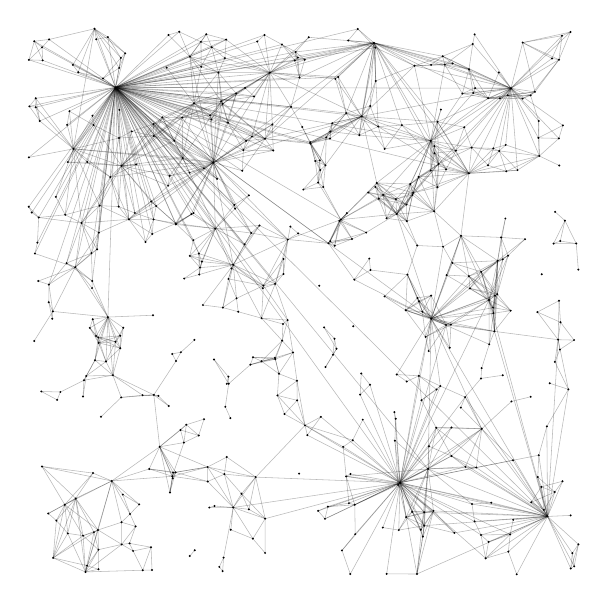
\begin{tikzpicture}[x=0.233333cm, y=0.233333cm]
% Generated by scripts/generate_sirg.py: seed=random, vertices=499, line width=0.2pt, opacity=0.28

% Vertices
\coordinate (v0) at (6.187895,0.34681128);
\coordinate (v1) at (-4.9246649,7.7157096);
\coordinate (v2) at (8.0825061,2.2555154);
\coordinate (v3) at (-6.2062779,2.6356043);
\coordinate (v4) at (9.2933321,-11.81425);
\coordinate (v5) at (7.2263402,-4.6365511);
\coordinate (v6) at (-13.645375,-13.799772);
\coordinate (v7) at (-4.324272,-9.2419295);
\coordinate (v8) at (-2.1027252,-11.665018);
\coordinate (v9) at (-14.212097,13.279046);
\coordinate (v10) at (2.3053997,-9.3633551);
\coordinate (v11) at (-8.9586616,-10.8881);
\coordinate (v12) at (-14.586965,11.214507);
\coordinate (v13) at (2.6878031,-1.1933304);
\coordinate (v14) at (10.827889,2.4475719);
\coordinate (v15) at (9.6429467,-4.0321706);
\coordinate (v16) at (-5.9382804,-13.385371);
\coordinate (v17) at (1.9316024,4.544822);
\coordinate (v18) at (-0.30832819,3.8595285);
\coordinate (v19) at (1.3418938,3.3194658);
\coordinate (v20) at (-0.36369653,-5.2239409);
\coordinate (v21) at (3.8945385,13.974207);
\coordinate (v22) at (-12.846271,7.7430553);
\coordinate (v23) at (3.6114299,10.793984);
\coordinate (v24) at (-5.2320466,-9.6428187);
\coordinate (v25) at (-7.3625997,14.662184);
\coordinate (v26) at (5.0003813,-6.2283624);
\coordinate (v27) at (-11.25068,2.9936355);
\coordinate (v28) at (3.8920526,6.390534);
\coordinate (v29) at (-0.88116809,-0.85846001);
\coordinate (v30) at (-0.32455475,13.424507);
\coordinate (v31) at (12.783088,9.9761868);
\coordinate (v32) at (7.1069568,8.6112685);
\coordinate (v33) at (8.7288818,9.6384238);
\coordinate (v34) at (-5.9552991,-1.9381421);
\coordinate (v35) at (6.3630775,-12.269011);
\coordinate (v36) at (-9.8525539,-10.353802);
\coordinate (v37) at (13.8409,-1.9241424);
\coordinate (v38) at (0.77950868,6.6266218);
\coordinate (v39) at (7.4619842,10.60196);
\coordinate (v40) at (12.342361,11.372252);
\coordinate (v41) at (7.5597227,13.502564);
\coordinate (v42) at (0.61989715,7.8006748);
\coordinate (v43) at (12.791073,-8.211057);
\coordinate (v44) at (-4.1053222,-3.9372694);
\coordinate (v45) at (-9.990475,-1.7115807);
\coordinate (v46) at (9.6825114,-6.7750835);
\coordinate (v47) at (-12.414135,-10.562198);
\coordinate (v48) at (-1.1024754,2.466792);
\coordinate (v49) at (10.29807,-0.18169927);
\coordinate (v50) at (3.2071329,-6.2745758);
\coordinate (v51) at (3.9123993,12.158208);
\coordinate (v52) at (-1.1358173,-1.0707928);
\coordinate (v53) at (5.5990183,-4.1998725);
\coordinate (v54) at (6.8149738,-7.726092);
\coordinate (v55) at (-10.451257,-9.6129262);
\coordinate (v56) at (-4.5989836,-14.293106);
\coordinate (v57) at (-8.6201571,3.3919367);
\coordinate (v58) at (-10.245218,-2.0356435);
\coordinate (v59) at (7.1102237,8.225204);
\coordinate (v60) at (10.37373,-1.4716719);
\coordinate (v61) at (11.586373,-14.695315);
\coordinate (v62) at (-1.1774056,-1.9765715);
\coordinate (v63) at (-10.768852,-3.1136633);
\coordinate (v64) at (0.35079454,8.8220847);
\coordinate (v65) at (3.1446323,10.230316);
\coordinate (v66) at (-3.1371388,8.8955939);
\coordinate (v67) at (14.052775,14.621322);
\coordinate (v68) at (-12.989356,4.8727599);
\coordinate (v69) at (1.4254021,9.0233675);
\coordinate (v70) at (8.1972072,-12.441206);
\coordinate (v71) at (11.394512,-11.727521);
\coordinate (v72) at (4.5051647,4.6839787);
\coordinate (v73) at (-9.8231628,-1.2746876);
\coordinate (v74) at (-6.5262492,-7.5256409);
\coordinate (v75) at (-7.7009837,10.178452);
\coordinate (v76) at (-11.177873,-13.353696);
\coordinate (v77) at (-6.218143,7.1647869);
\coordinate (v78) at (14.099717,9.736388);
\coordinate (v79) at (-8.3074602,5.5958063);
\coordinate (v80) at (6.9055113,7.2797991);
\coordinate (v81) at (-4.6492522,12.616445);
\coordinate (v82) at (-6.9653763,4.3477527);
\coordinate (v83) at (6.5570281,-12.045961);
\coordinate (v84) at (-3.3921117,-10.304954);
\coordinate (v85) at (8.100988,13.111847);
\coordinate (v86) at (-5.7201045,-7.1378947);
\coordinate (v87) at (-12.278548,12.636022);
\coordinate (v88) at (7.7458125,7.3421331);
\coordinate (v89) at (10.549064,2.3741416);
\coordinate (v90) at (2.3053785,10.410574);
\coordinate (v91) at (-3.8439849,-11.058199);
\coordinate (v92) at (-7.9147814,-4.9851853);
\coordinate (v93) at (-4.4188254,-14.523188);
\coordinate (v94) at (-5.4934559,-0.036512409);
\coordinate (v95) at (12.819164,8.0754977);
\coordinate (v96) at (6.4523908,-0.40140525);
\coordinate (v97) at (-3.2234546,3.2678238);
\coordinate (v98) at (6.9332458,-0.77896098);
\coordinate (v99) at (-3.6621276,0.32605638);
\coordinate (v100) at (-8.163136,-4.9287425);
\coordinate (v101) at (-6.7848839,14.835611);
\coordinate (v102) at (1.1507523,-11.675738);
\coordinate (v103) at (14.613683,-13.540136);
\coordinate (v104) at (-7.1597269,-2.6992622);
\coordinate (v105) at (-5.6934385,1.6214174);
\coordinate (v106) at (1.17478,7.5681656);
\coordinate (v107) at (-11.486448,-0.80842195);
\coordinate (v108) at (2.7727377,-10.91251);
\coordinate (v109) at (-2.1441474,14.659463);
\coordinate (v110) at (8.629269,11.47101);
\coordinate (v111) at (13.89125,0.19759305);
\coordinate (v112) at (-4.8161449,4.1209902);
\coordinate (v113) at (-6.709587,-6.8386608);
\coordinate (v114) at (-4.1902677,-4.3234517);
\coordinate (v115) at (9.6527574,1.7707328);
\coordinate (v116) at (-4.3670278,-13.786417);
\coordinate (v117) at (13.593305,3.3070297);
\coordinate (v118) at (-14.675123,-1.9938605);
\coordinate (v119) at (7.5807357,3.1342868);
\coordinate (v120) at (-6.0028372,4.9652687);
\coordinate (v121) at (-0.25943428,-9.2140903);
\coordinate (v122) at (2.5369468,-9.2319468);
\coordinate (v123) at (1.7117595,12.270533);
\coordinate (v124) at (-7.4664982,12.88205);
\coordinate (v125) at (-6.9806415,-9.1435206);
\coordinate (v126) at (-6.5131001,1.4038602);
\coordinate (v127) at (7.0570499,-11.241349);
\coordinate (v128) at (-11.112228,5.3703557);
\coordinate (v129) at (-3.6766245,11.473726);
\coordinate (v130) at (-14.806557,4.9974151);
\coordinate (v131) at (-4.4939356,11.048105);
\coordinate (v132) at (-1.1087998,1.6514002);
\coordinate (v133) at (-2.2401704,0.87629977);
\coordinate (v134) at (6.6258347,-1.7723213);
\coordinate (v135) at (10.205484,-10.796922);
\coordinate (v136) at (5.2352411,-9.7130198);
\coordinate (v137) at (-7.3027443,6.9951066);
\coordinate (v138) at (2.1411575,-7.7561479);
\coordinate (v139) at (4.0493943,9.6767372);
\coordinate (v140) at (-3.739547,5.2065953);
\coordinate (v141) at (-14.286738,-4.7421628);
\coordinate (v142) at (-1.355779,-3.7783691);
\coordinate (v143) at (3.0196627,9.2081051);
\coordinate (v144) at (-4.1931945,-8.3125805);
\coordinate (v145) at (-5.1439518,-11.061524);
\coordinate (v146) at (10.670533,11.205329);
\coordinate (v147) at (-9.3645438,9.4127812);
\coordinate (v148) at (1.0601173,6.3843688);
\coordinate (v149) at (-7.8462157,-7.7528066);
\coordinate (v150) at (-11.645719,-1.2877733);
\coordinate (v151) at (6.2612921,-3.8894869);
\coordinate (v152) at (13.386892,-4.2965446);
\coordinate (v153) at (-14.369742,9.9797584);
\coordinate (v154) at (11.904666,11.196892);
\coordinate (v155) at (-5.235357,-8.853755);
\coordinate (v156) at (10.077328,0.23655451);
\coordinate (v157) at (5.0573228,-3.820413);
\coordinate (v158) at (-1.7137464,9.7928381);
\coordinate (v159) at (1.6696038,-1.8730489);
\coordinate (v160) at (-12.100314,4.4236855);
\coordinate (v161) at (13.658127,-10.216674);
\coordinate (v162) at (-9.9894951,-2.3879933);
\coordinate (v163) at (-5.1032721,10.287804);
\coordinate (v164) at (6.0243803,12.983486);
\coordinate (v165) at (-4.2959752,13.396555);
\coordinate (v166) at (2.7973301,-12.507512);
\coordinate (v167) at (6.7599963,-8.9555693);
\coordinate (v168) at (-7.3849953,6.4542965);
\coordinate (v169) at (-9.9249349,7.5377423);
\coordinate (v170) at (7.7691691,1.5915331);
\coordinate (v171) at (-2.9072106,-3.2830472);
\coordinate (v172) at (9.0407982,0.86955395);
\coordinate (v173) at (-4.4164194,10.911463);
\coordinate (v174) at (-6.394337,-6.5524657);
\coordinate (v175) at (-8.7767283,-4.94555);
\coordinate (v176) at (-14.668872,14.317281);
\coordinate (v177) at (-8.1812419,4.6235351);
\coordinate (v178) at (8.546663,-5.6155818);
\coordinate (v179) at (-7.1344991,-9.4626003);
\coordinate (v180) at (-4.8640172,-10.976557);
\coordinate (v181) at (-5.3060321,14.699642);
\coordinate (v182) at (10.636355,8.351249);
\coordinate (v183) at (-13.661229,-0.38537112);
\coordinate (v184) at (-4.8867694,-2.998961);
\coordinate (v185) at (14.705773,-1.9470243);
\coordinate (v186) at (-6.9566251,-3.0850525);
\coordinate (v187) at (-8.0360554,5.3491384);
\coordinate (v188) at (-4.1298703,9.8823628);
\coordinate (v189) at (14.08437,-9.6287195);
\coordinate (v190) at (13.227688,-6.6415984);
\coordinate (v191) at (1.3104947,-11.010587);
\coordinate (v192) at (-5.5889315,12.929768);
\coordinate (v193) at (10.824254,-3.8599868);
\coordinate (v194) at (5.5444215,-0.32315314);
\coordinate (v195) at (10.530824,0.5524012);
\coordinate (v196) at (-1.1942376,14.142973);
\coordinate (v197) at (-1.662846,8.3726708);
\coordinate (v198) at (0.83730513,1.0137461);
\coordinate (v199) at (-3.7776798,5.4127185);
\coordinate (v200) at (7.7432082,-1.1222029);
\coordinate (v201) at (5.9488807,6.0707728);
\coordinate (v202) at (-6.5918408,7.9673711);
\coordinate (v203) at (-6.2027078,13.482614);
\coordinate (v204) at (9.1914909,14.167495);
\coordinate (v205) at (-9.5207124,4.6280503);
\coordinate (v206) at (5.5893004,5.4285503);
\coordinate (v207) at (-14.250108,-8.8259231);
\coordinate (v208) at (2.0771386,-13.391992);
\coordinate (v209) at (2.4567243,-10.821071);
\coordinate (v210) at (-2.4127038,4.2918175);
\coordinate (v211) at (-11.798455,-14.223132);
\coordinate (v212) at (-12.015539,-12.591616);
\coordinate (v213) at (-6.9720178,4.40579);
\coordinate (v214) at (-7.1115281,-9.1596184);
\coordinate (v215) at (0.35675773,8.7468027);
\coordinate (v216) at (-11.309622,-1.7211063);
\coordinate (v217) at (-5.6505191,1.9975089);
\coordinate (v218) at (-12.878241,9.7686644);
\coordinate (v219) at (-9.9195299,-11.858766);
\coordinate (v220) at (-14.428389,4.7260365);
\coordinate (v221) at (11.097693,11.381954);
\coordinate (v222) at (-11.525674,0.88559572);
\coordinate (v223) at (-11.19879,-12.281657);
\coordinate (v224) at (-9.7244081,13.663337);
\coordinate (v225) at (3.6001634,-4.372949);
\coordinate (v226) at (-11.156106,3.9040857);
\coordinate (v227) at (-0.86953203,3.5278168);
\coordinate (v228) at (-14.961963,7.9991132);
\coordinate (v229) at (5.9114489,5.9550662);
\coordinate (v230) at (-5.0118555,13.997218);
\coordinate (v231) at (-0.23612778,12.34402);
\coordinate (v232) at (14.714492,-14.257744);
\coordinate (v233) at (-1.4374945,-4.9592249);
\coordinate (v234) at (-6.6198448,10.168731);
\coordinate (v235) at (13.901226,7.5574298);
\coordinate (v236) at (6.9319061,0.47593289);
\coordinate (v237) at (-11.188553,-1.811626);
\coordinate (v238) at (-12.542082,8.4624621);
\coordinate (v239) at (12.926626,-9.9327769);
\coordinate (v240) at (3.3916653,3.9086181);
\coordinate (v241) at (7.428525,-4.4478319);
\coordinate (v242) at (-3.1936556,11.780442);
\coordinate (v243) at (13.880722,9.0298149);
\coordinate (v244) at (12.039169,3.548358);
\coordinate (v245) at (-14.247069,13.98847);
\coordinate (v246) at (4.956967,-7.4212557);
\coordinate (v247) at (-6.0132146,3.4890354);
\coordinate (v248) at (-5.5975991,14.285637);
\coordinate (v249) at (10.091044,-2.1781075);
\coordinate (v250) at (1.7785184,-2.4193743);
\coordinate (v251) at (-10.03957,10.581262);
\coordinate (v252) at (14.524462,-14.378257);
\coordinate (v253) at (13.067142,-11.187189);
\coordinate (v254) at (-8.263423,-14.46006);
\coordinate (v255) at (3.5101512,6.0888577);
\coordinate (v256) at (-7.1565587,-9.3579762);
\coordinate (v257) at (-14.635126,2.7639446);
\coordinate (v258) at (-11.423874,-12.402281);
\coordinate (v259) at (11.913589,14.245515);
\coordinate (v260) at (-9.1231045,7.6162281);
\coordinate (v261) at (-11.44747,9.7624567);
\coordinate (v262) at (-9.485862,-13.010075);
\coordinate (v263) at (2.6613454,-7.3959663);
\coordinate (v264) at (13.97062,-0.97740994);
\coordinate (v265) at (-0.49019801,13.272123);
\coordinate (v266) at (5.5673963,-11.584773);
\coordinate (v267) at (-11.03619,-6.1191505);
\coordinate (v268) at (-2.7615036,-2.8798922);
\coordinate (v269) at (-14.499808,3.3572676);
\coordinate (v270) at (-12.017314,-5.0159844);
\coordinate (v271) at (14.827554,3.3065858);
\coordinate (v272) at (8.9830622,1.5301407);
\coordinate (v273) at (4.0774079,5.7507835);
\coordinate (v274) at (1.8719874,12.375587);
\coordinate (v275) at (-11.787436,7.7454462);
\coordinate (v276) at (-0.73220886,4.2305782);
\coordinate (v277) at (-11.393264,14.99778);
\coordinate (v278) at (-5.5534581,2.3253808);
\coordinate (v279) at (4.3151058,5.9550475);
\coordinate (v280) at (-2.7117914,11.313415);
\coordinate (v281) at (12.38218,-10.771605);
\coordinate (v282) at (-8.3154006,-13.218879);
\coordinate (v283) at (-13.011385,-10.904971);
\coordinate (v284) at (-0.37289866,-4.161171);
\coordinate (v285) at (8.5540378,3.7306439);
\coordinate (v286) at (-11.497341,10.265004);
\coordinate (v287) at (14.939302,1.8899008);
\coordinate (v288) at (9.3248289,11.769794);
\coordinate (v289) at (-10.248969,11.809405);
\coordinate (v290) at (-0.44424706,13.736432);
\coordinate (v291) at (-8.7668043,-14.470741);
\coordinate (v292) at (0.78209527,-11.23972);
\coordinate (v293) at (1.1017215,-1.254019);
\coordinate (v294) at (-11.515228,1.2651435);
\coordinate (v295) at (-14.453199,1.2664593);
\coordinate (v296) at (-2.199312,1.0196181);
\coordinate (v297) at (0.86750385,7.8361277);
\coordinate (v298) at (-0.69508328,10.748112);
\coordinate (v299) at (0.047005814,13.314155);
\coordinate (v300) at (13.885546,13.313724);
\coordinate (v301) at (5.7951577,6.5477021);
\coordinate (v302) at (3.5618992,2.4881888);
\coordinate (v303) at (5.1302107,-9.8208135);
\coordinate (v304) at (-14.961047,13.304672);
\coordinate (v305) at (-3.3529773,7.2694328);
\coordinate (v306) at (1.5889954,-2.7460512);
\coordinate (v307) at (7.3336471,7.6427814);
\coordinate (v308) at (12.946248,1.6375663);
\coordinate (v309) at (10.031399,11.218356);
\coordinate (v310) at (-2.8225955,9.1397892);
\coordinate (v311) at (-11.178566,-14.419747);
\coordinate (v312) at (-12.43736,2.0192149);
\coordinate (v313) at (3.1254709,-3.7690428);
\coordinate (v314) at (-9.9388112,-5.064957);
\coordinate (v315) at (8.7780432,-5.0491608);
\coordinate (v316) at (8.9825299,7.1304866);
\coordinate (v317) at (-2.1114046,-13.528686);
\coordinate (v318) at (10.319175,-0.48270908);
\coordinate (v319) at (-10.530995,6.9263625);
\coordinate (v320) at (-13.882446,0.11641589);
\coordinate (v321) at (-10.927684,12.29251);
\coordinate (v322) at (3.6279918,1.8686506);
\coordinate (v323) at (11.381217,-8.4875026);
\coordinate (v324) at (-10.662958,-0.69304041);
\coordinate (v325) at (13.266429,-11.544958);
\coordinate (v326) at (-13.424915,-5.1991409);
\coordinate (v327) at (-10.055619,9.051227);
\coordinate (v328) at (8.7953241,-8.8418147);
\coordinate (v329) at (6.2469282,6.9329165);
\coordinate (v330) at (5.0105963,5.7214183);
\coordinate (v331) at (-1.5503652,-2.9835445);
\coordinate (v332) at (-13.497967,5.8488531);
\coordinate (v333) at (-5.4330161,-6.2486786);
\coordinate (v334) at (1.4412635,9.408323);
\coordinate (v335) at (7.6718258,13.045349);
\coordinate (v336) at (-9.4571813,-11.409279);
\coordinate (v337) at (-2.9870125,-11.158385);
\coordinate (v338) at (-8.2505305,3.8316693);
\coordinate (v339) at (11.018811,7.2388031);
\coordinate (v340) at (-14.970037,5.3091784);
\coordinate (v341) at (-2.8626253,3.8807903);
\coordinate (v342) at (-3.5723856,-0.4030994);
\coordinate (v343) at (5.8938415,-11.291249);
\coordinate (v344) at (-7.2877044,-10.240321);
\coordinate (v345) at (-11.294396,14.42581);
\coordinate (v346) at (-11.841067,-3.8990998);
\coordinate (v347) at (-4.1021887,1.3842331);
\coordinate (v348) at (-3.9988137,-6.1904471);
\coordinate (v349) at (10.315109,8.484223);
\coordinate (v350) at (13.677486,5.0340306);
\coordinate (v351) at (-0.58946803,-2.6184114);
\coordinate (v352) at (7.0937759,5.0650318);
\coordinate (v353) at (5.6408784,1.6187051);
\coordinate (v354) at (-7.3541433,-5.5337766);
\coordinate (v355) at (-1.8475425,12.61001);
\coordinate (v356) at (-4.7226544,6.8283215);
\coordinate (v357) at (-10.391915,-3.8591704);
\coordinate (v358) at (-2.7730747,-12.755447);
\coordinate (v359) at (10.96984,4.671529);
\coordinate (v360) at (11.259285,-0.34550998);
\coordinate (v361) at (1.2198301,9.0884927);
\coordinate (v362) at (10.987533,8.676075);
\coordinate (v363) at (-13.905822,-11.383796);
\coordinate (v364) at (11.230289,-12.523758);
\coordinate (v365) at (-10.665992,14.543394);
\coordinate (v366) at (6.2671884,0.17160791);
\coordinate (v367) at (14.946022,-13.062832);
\coordinate (v368) at (1.6800556,3.1881111);
\coordinate (v369) at (-3.8385775,2.151968);
\coordinate (v370) at (-11.883989,-14.566117);
\coordinate (v371) at (9.2952584,14.68886);
\coordinate (v372) at (10.61398,12.620821);
\coordinate (v373) at (-4.4066516,-0.17555484);
\coordinate (v374) at (-14.934739,10.774007);
\coordinate (v375) at (10.7407,3.6413881);
\coordinate (v376) at (11.275848,11.758861);
\coordinate (v377) at (-9.2912388,-13.424178);
\coordinate (v378) at (-10.075829,5.3194453);
\coordinate (v379) at (-13.690682,-0.78592346);
\coordinate (v380) at (-3.9368476,1.955784);
\coordinate (v381) at (-5.4378553,7.4006924);
\coordinate (v382) at (13.507318,13.383836);
\coordinate (v383) at (-14.590531,10.725511);
\coordinate (v384) at (9.2221464,11.502358);
\coordinate (v385) at (0.064550253,-6.5874873);
\coordinate (v386) at (6.9288373,13.028253);
\coordinate (v387) at (9.129924,8.5318135);
\coordinate (v388) at (12.711892,-0.41977302);
\coordinate (v389) at (0.19007886,-7.1185071);
\coordinate (v390) at (0.27197987,14.535495);
\coordinate (v391) at (6.9084387,8.8966032);
\coordinate (v392) at (12.347249,-5.0327261);
\coordinate (v393) at (14.21171,4.5549142);
\coordinate (v394) at (-4.2733215,-5.5777258);
\coordinate (v395) at (11.302275,-5.2828573);
\coordinate (v396) at (-2.990708,5.9356706);
\coordinate (v397) at (12.732567,-9.400923);
\coordinate (v398) at (13.957151,3.4455775);
\coordinate (v399) at (-9.9578236,13.413469);
\coordinate (v400) at (-7.0469324,8.9027753);
\coordinate (v401) at (-8.1852475,9.812367);
\coordinate (v402) at (4.4026348,8.461732);
\coordinate (v403) at (9.1528609,-10.872451);
\coordinate (v404) at (-4.2277568,14.409025);
\coordinate (v405) at (-2.3012663,-0.75243584);
\coordinate (v406) at (-5.0306765,10.062065);
\coordinate (v407) at (2.528891,-14.678766);
\coordinate (v408) at (-11.557443,2.7894088);
\coordinate (v409) at (-8.1689185,9.1634658);
\coordinate (v410) at (8.9902461,12.800478);
\coordinate (v411) at (-2.6179808,-9.4032942);
\coordinate (v412) at (3.8172639,14.231125);
\coordinate (v413) at (-13.46749,-11.768824);
\coordinate (v414) at (13.664371,-3.1266009);
\coordinate (v415) at (-6.2090803,-13.702052);
\coordinate (v416) at (6.4046758,-5.2191129);
\coordinate (v417) at (-12.916252,2.2416218);
\coordinate (v418) at (-11.168919,-2.0948265);
\coordinate (v419) at (6.7938123,-2.5416673);
\coordinate (v420) at (5.6097017,4.5266783);
\coordinate (v421) at (-3.2893846,8.3890791);
\coordinate (v422) at (-10.050002,12.865076);
\coordinate (v423) at (14.511235,14.820322);
\coordinate (v424) at (8.0070877,-1.1025973);
\coordinate (v425) at (9.6783792,-3.4742719);
\coordinate (v426) at (-12.571222,13.032563);
\coordinate (v427) at (11.629586,7.3039025);
\coordinate (v428) at (10.052947,-12.928162);
\coordinate (v429) at (-13.861333,14.416824);
\coordinate (v430) at (-11.365818,-3.0375163);
\coordinate (v431) at (2.746665,1.3439688);
\coordinate (v432) at (4.9337343,-5.8670823);
\coordinate (v433) at (-3.9728705,-12.268388);
\coordinate (v434) at (-1.0505239,-5.9724153);
\coordinate (v435) at (3.0660314,-4.9139288);
\coordinate (v436) at (12.580288,11.564756);
\coordinate (v437) at (2.6222018,3.5564772);
\coordinate (v438) at (9.6439914,-12.55224);
\coordinate (v439) at (9.3898055,-8.882277);
\coordinate (v440) at (3.9693817,6.6092739);
\coordinate (v441) at (-2.5335222,14.305902);
\coordinate (v442) at (0.89469502,7.3114975);
\coordinate (v443) at (2.9387635,14.987024);
\coordinate (v444) at (-8.2134922,-0.59358394);
\coordinate (v445) at (2.4166685,14.360456);
\coordinate (v446) at (-2.3009815,-3.0957909);
\coordinate (v447) at (14.399103,-4.6282946);
\coordinate (v448) at (5.1694753,-12.286543);
\coordinate (v449) at (13.937715,-2.4597286);
\coordinate (v450) at (11.117639,2.6491089);
\coordinate (v451) at (7.276576,6.3757244);
\coordinate (v452) at (-13.875218,1.0771606);
\coordinate (v453) at (10.407822,0.471812);
\coordinate (v454) at (-11.474426,-9.185126);
\coordinate (v455) at (6.5571337,-11.320034);
\coordinate (v456) at (0.92655282,-6.1243464);
\coordinate (v457) at (5.3366592,9.7506631);
\coordinate (v458) at (1.4419158,3.4369362);
\coordinate (v459) at (-6.1184341,4.9109611);
\coordinate (v460) at (-0.088385277,9.6516411);
\coordinate (v461) at (7.2068072,-6.7199427);
\coordinate (v462) at (-9.195608,4.9706522);
\coordinate (v463) at (2.3457934,4.9644305);
\coordinate (v464) at (-1.5720922,-2.9125229);
\coordinate (v465) at (-5.7122301,2.761486);
\coordinate (v466) at (8.0338434,-8.2526662);
\coordinate (v467) at (-0.025186033,6.2497403);
\coordinate (v468) at (11.132038,-13.460235);
\coordinate (v469) at (-11.966361,-4.1323891);
\coordinate (v470) at (8.036301,-6.703945);
\coordinate (v471) at (6.1695133,3.2021505);
\coordinate (v472) at (-13.250285,-4.7720956);
\coordinate (v473) at (-5.9762783,10.942537);
\coordinate (v474) at (-2.1112497,9.013372);
\coordinate (v475) at (6.1545374,-14.676614);
\coordinate (v476) at (14.521415,-11.487373);
\coordinate (v477) at (-1.561254,1.1086963);
\coordinate (v478) at (4.3954572,0.43424094);
\coordinate (v479) at (-6.6870254,-2.6037812);
\coordinate (v480) at (-9.9116526,-13.066676);
\coordinate (v481) at (1.1826117,-3.4126882);
\coordinate (v482) at (4.5084302,-14.672966);
\coordinate (v483) at (-12.759097,10.510235);
\coordinate (v484) at (-12.847121,-12.466964);
\coordinate (v485) at (-8.4162418,-8.9599362);
\coordinate (v486) at (8.2723487,8.3645385);
\coordinate (v487) at (5.0551003,4.9154723);
\coordinate (v488) at (9.895832,-13.822563);
\coordinate (v489) at (2.0117363,4.610109);
\coordinate (v490) at (4.2981865,-12.149633);
\coordinate (v491) at (10.023471,7.5688051);
\coordinate (v492) at (7.9430108,-2.3651914);
\coordinate (v493) at (7.2778286,9.9321393);
\coordinate (v494) at (-9.1560182,-12.087326);
\coordinate (v495) at (12.763677,9.0585144);
\coordinate (v496) at (-4.0901729,-4.3221429);
\coordinate (v497) at (1.5475183,9.8558258);
\coordinate (v498) at (6.4803668,-12.645026);

% Edges
\draw[line width=0.2pt, opacity=0.28] (v0) -- (v96);
\draw[line width=0.2pt, opacity=0.28] (v0) -- (v98);
\draw[line width=0.2pt, opacity=0.28] (v0) -- (v194);
\draw[line width=0.2pt, opacity=0.28] (v0) -- (v236);
\draw[line width=0.2pt, opacity=0.28] (v0) -- (v353);
\draw[line width=0.2pt, opacity=0.28] (v0) -- (v366);
\draw[line width=0.2pt, opacity=0.28] (v1) -- (v65);
\draw[line width=0.2pt, opacity=0.28] (v1) -- (v66);
\draw[line width=0.2pt, opacity=0.28] (v1) -- (v75);
\draw[line width=0.2pt, opacity=0.28] (v1) -- (v77);
\draw[line width=0.2pt, opacity=0.28] (v1) -- (v79);
\draw[line width=0.2pt, opacity=0.28] (v1) -- (v81);
\draw[line width=0.2pt, opacity=0.28] (v1) -- (v82);
\draw[line width=0.2pt, opacity=0.28] (v1) -- (v112);
\draw[line width=0.2pt, opacity=0.28] (v1) -- (v120);
\draw[line width=0.2pt, opacity=0.28] (v1) -- (v129);
\draw[line width=0.2pt, opacity=0.28] (v1) -- (v131);
\draw[line width=0.2pt, opacity=0.28] (v1) -- (v137);
\draw[line width=0.2pt, opacity=0.28] (v1) -- (v140);
\draw[line width=0.2pt, opacity=0.28] (v1) -- (v158);
\draw[line width=0.2pt, opacity=0.28] (v1) -- (v163);
\draw[line width=0.2pt, opacity=0.28] (v1) -- (v168);
\draw[line width=0.2pt, opacity=0.28] (v1) -- (v169);
\draw[line width=0.2pt, opacity=0.28] (v1) -- (v173);
\draw[line width=0.2pt, opacity=0.28] (v1) -- (v187);
\draw[line width=0.2pt, opacity=0.28] (v1) -- (v188);
\draw[line width=0.2pt, opacity=0.28] (v1) -- (v197);
\draw[line width=0.2pt, opacity=0.28] (v1) -- (v199);
\draw[line width=0.2pt, opacity=0.28] (v1) -- (v202);
\draw[line width=0.2pt, opacity=0.28] (v1) -- (v203);
\draw[line width=0.2pt, opacity=0.28] (v1) -- (v205);
\draw[line width=0.2pt, opacity=0.28] (v1) -- (v213);
\draw[line width=0.2pt, opacity=0.28] (v1) -- (v227);
\draw[line width=0.2pt, opacity=0.28] (v1) -- (v234);
\draw[line width=0.2pt, opacity=0.28] (v1) -- (v238);
\draw[line width=0.2pt, opacity=0.28] (v1) -- (v289);
\draw[line width=0.2pt, opacity=0.28] (v1) -- (v305);
\draw[line width=0.2pt, opacity=0.28] (v1) -- (v310);
\draw[line width=0.2pt, opacity=0.28] (v1) -- (v319);
\draw[line width=0.2pt, opacity=0.28] (v1) -- (v341);
\draw[line width=0.2pt, opacity=0.28] (v1) -- (v355);
\draw[line width=0.2pt, opacity=0.28] (v1) -- (v356);
\draw[line width=0.2pt, opacity=0.28] (v1) -- (v369);
\draw[line width=0.2pt, opacity=0.28] (v1) -- (v381);
\draw[line width=0.2pt, opacity=0.28] (v1) -- (v396);
\draw[line width=0.2pt, opacity=0.28] (v1) -- (v400);
\draw[line width=0.2pt, opacity=0.28] (v1) -- (v401);
\draw[line width=0.2pt, opacity=0.28] (v1) -- (v406);
\draw[line width=0.2pt, opacity=0.28] (v1) -- (v409);
\draw[line width=0.2pt, opacity=0.28] (v1) -- (v412);
\draw[line width=0.2pt, opacity=0.28] (v1) -- (v421);
\draw[line width=0.2pt, opacity=0.28] (v1) -- (v459);
\draw[line width=0.2pt, opacity=0.28] (v1) -- (v473);
\draw[line width=0.2pt, opacity=0.28] (v1) -- (v474);
\draw[line width=0.2pt, opacity=0.28] (v2) -- (v89);
\draw[line width=0.2pt, opacity=0.28] (v2) -- (v98);
\draw[line width=0.2pt, opacity=0.28] (v2) -- (v115);
\draw[line width=0.2pt, opacity=0.28] (v2) -- (v119);
\draw[line width=0.2pt, opacity=0.28] (v2) -- (v170);
\draw[line width=0.2pt, opacity=0.28] (v2) -- (v272);
\draw[line width=0.2pt, opacity=0.28] (v2) -- (v285);
\draw[line width=0.2pt, opacity=0.28] (v3) -- (v112);
\draw[line width=0.2pt, opacity=0.28] (v3) -- (v217);
\draw[line width=0.2pt, opacity=0.28] (v3) -- (v247);
\draw[line width=0.2pt, opacity=0.28] (v3) -- (v278);
\draw[line width=0.2pt, opacity=0.28] (v3) -- (v369);
\draw[line width=0.2pt, opacity=0.28] (v3) -- (v465);
\draw[line width=0.2pt, opacity=0.28] (v4) -- (v136);
\draw[line width=0.2pt, opacity=0.28] (v4) -- (v325);
\draw[line width=0.2pt, opacity=0.28] (v4) -- (v403);
\draw[line width=0.2pt, opacity=0.28] (v4) -- (v438);
\draw[line width=0.2pt, opacity=0.28] (v5) -- (v136);
\draw[line width=0.2pt, opacity=0.28] (v5) -- (v151);
\draw[line width=0.2pt, opacity=0.28] (v5) -- (v241);
\draw[line width=0.2pt, opacity=0.28] (v5) -- (v416);
\draw[line width=0.2pt, opacity=0.28] (v6) -- (v47);
\draw[line width=0.2pt, opacity=0.28] (v6) -- (v211);
\draw[line width=0.2pt, opacity=0.28] (v6) -- (v212);
\draw[line width=0.2pt, opacity=0.28] (v6) -- (v223);
\draw[line width=0.2pt, opacity=0.28] (v6) -- (v283);
\draw[line width=0.2pt, opacity=0.28] (v6) -- (v370);
\draw[line width=0.2pt, opacity=0.28] (v6) -- (v413);
\draw[line width=0.2pt, opacity=0.28] (v6) -- (v484);
\draw[line width=0.2pt, opacity=0.28] (v7) -- (v24);
\draw[line width=0.2pt, opacity=0.28] (v7) -- (v84);
\draw[line width=0.2pt, opacity=0.28] (v7) -- (v91);
\draw[line width=0.2pt, opacity=0.28] (v7) -- (v144);
\draw[line width=0.2pt, opacity=0.28] (v7) -- (v155);
\draw[line width=0.2pt, opacity=0.28] (v7) -- (v411);
\draw[line width=0.2pt, opacity=0.28] (v8) -- (v84);
\draw[line width=0.2pt, opacity=0.28] (v8) -- (v91);
\draw[line width=0.2pt, opacity=0.28] (v8) -- (v136);
\draw[line width=0.2pt, opacity=0.28] (v8) -- (v317);
\draw[line width=0.2pt, opacity=0.28] (v8) -- (v337);
\draw[line width=0.2pt, opacity=0.28] (v8) -- (v358);
\draw[line width=0.2pt, opacity=0.28] (v8) -- (v411);
\draw[line width=0.2pt, opacity=0.28] (v9) -- (v176);
\draw[line width=0.2pt, opacity=0.28] (v9) -- (v245);
\draw[line width=0.2pt, opacity=0.28] (v9) -- (v289);
\draw[line width=0.2pt, opacity=0.28] (v9) -- (v304);
\draw[line width=0.2pt, opacity=0.28] (v10) -- (v108);
\draw[line width=0.2pt, opacity=0.28] (v10) -- (v122);
\draw[line width=0.2pt, opacity=0.28] (v10) -- (v136);
\draw[line width=0.2pt, opacity=0.28] (v10) -- (v138);
\draw[line width=0.2pt, opacity=0.28] (v10) -- (v167);
\draw[line width=0.2pt, opacity=0.28] (v10) -- (v209);
\draw[line width=0.2pt, opacity=0.28] (v10) -- (v303);
\draw[line width=0.2pt, opacity=0.28] (v11) -- (v36);
\draw[line width=0.2pt, opacity=0.28] (v11) -- (v55);
\draw[line width=0.2pt, opacity=0.28] (v11) -- (v336);
\draw[line width=0.2pt, opacity=0.28] (v12) -- (v153);
\draw[line width=0.2pt, opacity=0.28] (v12) -- (v238);
\draw[line width=0.2pt, opacity=0.28] (v12) -- (v289);
\draw[line width=0.2pt, opacity=0.28] (v12) -- (v374);
\draw[line width=0.2pt, opacity=0.28] (v12) -- (v383);
\draw[line width=0.2pt, opacity=0.28] (v14) -- (v89);
\draw[line width=0.2pt, opacity=0.28] (v14) -- (v115);
\draw[line width=0.2pt, opacity=0.28] (v14) -- (v156);
\draw[line width=0.2pt, opacity=0.28] (v14) -- (v195);
\draw[line width=0.2pt, opacity=0.28] (v14) -- (v375);
\draw[line width=0.2pt, opacity=0.28] (v14) -- (v450);
\draw[line width=0.2pt, opacity=0.28] (v15) -- (v193);
\draw[line width=0.2pt, opacity=0.28] (v15) -- (v315);
\draw[line width=0.2pt, opacity=0.28] (v15) -- (v425);
\draw[line width=0.2pt, opacity=0.28] (v16) -- (v415);
\draw[line width=0.2pt, opacity=0.28] (v17) -- (v19);
\draw[line width=0.2pt, opacity=0.28] (v17) -- (v240);
\draw[line width=0.2pt, opacity=0.28] (v17) -- (v368);
\draw[line width=0.2pt, opacity=0.28] (v17) -- (v437);
\draw[line width=0.2pt, opacity=0.28] (v17) -- (v458);
\draw[line width=0.2pt, opacity=0.28] (v17) -- (v463);
\draw[line width=0.2pt, opacity=0.28] (v17) -- (v489);
\draw[line width=0.2pt, opacity=0.28] (v18) -- (v19);
\draw[line width=0.2pt, opacity=0.28] (v18) -- (v227);
\draw[line width=0.2pt, opacity=0.28] (v18) -- (v276);
\draw[line width=0.2pt, opacity=0.28] (v19) -- (v227);
\draw[line width=0.2pt, opacity=0.28] (v19) -- (v240);
\draw[line width=0.2pt, opacity=0.28] (v19) -- (v289);
\draw[line width=0.2pt, opacity=0.28] (v19) -- (v368);
\draw[line width=0.2pt, opacity=0.28] (v19) -- (v431);
\draw[line width=0.2pt, opacity=0.28] (v19) -- (v437);
\draw[line width=0.2pt, opacity=0.28] (v19) -- (v458);
\draw[line width=0.2pt, opacity=0.28] (v19) -- (v463);
\draw[line width=0.2pt, opacity=0.28] (v19) -- (v489);
\draw[line width=0.2pt, opacity=0.28] (v20) -- (v233);
\draw[line width=0.2pt, opacity=0.28] (v20) -- (v284);
\draw[line width=0.2pt, opacity=0.28] (v20) -- (v385);
\draw[line width=0.2pt, opacity=0.28] (v20) -- (v434);
\draw[line width=0.2pt, opacity=0.28] (v21) -- (v51);
\draw[line width=0.2pt, opacity=0.28] (v21) -- (v65);
\draw[line width=0.2pt, opacity=0.28] (v21) -- (v164);
\draw[line width=0.2pt, opacity=0.28] (v21) -- (v289);
\draw[line width=0.2pt, opacity=0.28] (v21) -- (v412);
\draw[line width=0.2pt, opacity=0.28] (v21) -- (v443);
\draw[line width=0.2pt, opacity=0.28] (v21) -- (v445);
\draw[line width=0.2pt, opacity=0.28] (v22) -- (v169);
\draw[line width=0.2pt, opacity=0.28] (v22) -- (v238);
\draw[line width=0.2pt, opacity=0.28] (v22) -- (v275);
\draw[line width=0.2pt, opacity=0.28] (v22) -- (v289);
\draw[line width=0.2pt, opacity=0.28] (v23) -- (v51);
\draw[line width=0.2pt, opacity=0.28] (v23) -- (v65);
\draw[line width=0.2pt, opacity=0.28] (v23) -- (v90);
\draw[line width=0.2pt, opacity=0.28] (v23) -- (v139);
\draw[line width=0.2pt, opacity=0.28] (v23) -- (v143);
\draw[line width=0.2pt, opacity=0.28] (v23) -- (v412);
\draw[line width=0.2pt, opacity=0.28] (v24) -- (v91);
\draw[line width=0.2pt, opacity=0.28] (v24) -- (v125);
\draw[line width=0.2pt, opacity=0.28] (v24) -- (v155);
\draw[line width=0.2pt, opacity=0.28] (v24) -- (v256);
\draw[line width=0.2pt, opacity=0.28] (v25) -- (v101);
\draw[line width=0.2pt, opacity=0.28] (v25) -- (v203);
\draw[line width=0.2pt, opacity=0.28] (v25) -- (v289);
\draw[line width=0.2pt, opacity=0.28] (v26) -- (v136);
\draw[line width=0.2pt, opacity=0.28] (v26) -- (v246);
\draw[line width=0.2pt, opacity=0.28] (v26) -- (v432);
\draw[line width=0.2pt, opacity=0.28] (v27) -- (v160);
\draw[line width=0.2pt, opacity=0.28] (v27) -- (v226);
\draw[line width=0.2pt, opacity=0.28] (v27) -- (v289);
\draw[line width=0.2pt, opacity=0.28] (v27) -- (v312);
\draw[line width=0.2pt, opacity=0.28] (v27) -- (v408);
\draw[line width=0.2pt, opacity=0.28] (v28) -- (v255);
\draw[line width=0.2pt, opacity=0.28] (v28) -- (v273);
\draw[line width=0.2pt, opacity=0.28] (v28) -- (v279);
\draw[line width=0.2pt, opacity=0.28] (v28) -- (v330);
\draw[line width=0.2pt, opacity=0.28] (v28) -- (v440);
\draw[line width=0.2pt, opacity=0.28] (v28) -- (v487);
\draw[line width=0.2pt, opacity=0.28] (v29) -- (v52);
\draw[line width=0.2pt, opacity=0.28] (v29) -- (v62);
\draw[line width=0.2pt, opacity=0.28] (v29) -- (v296);
\draw[line width=0.2pt, opacity=0.28] (v29) -- (v351);
\draw[line width=0.2pt, opacity=0.28] (v29) -- (v405);
\draw[line width=0.2pt, opacity=0.28] (v29) -- (v477);
\draw[line width=0.2pt, opacity=0.28] (v30) -- (v196);
\draw[line width=0.2pt, opacity=0.28] (v30) -- (v231);
\draw[line width=0.2pt, opacity=0.28] (v30) -- (v265);
\draw[line width=0.2pt, opacity=0.28] (v30) -- (v290);
\draw[line width=0.2pt, opacity=0.28] (v30) -- (v299);
\draw[line width=0.2pt, opacity=0.28] (v30) -- (v355);
\draw[line width=0.2pt, opacity=0.28] (v30) -- (v412);
\draw[line width=0.2pt, opacity=0.28] (v31) -- (v40);
\draw[line width=0.2pt, opacity=0.28] (v31) -- (v95);
\draw[line width=0.2pt, opacity=0.28] (v31) -- (v376);
\draw[line width=0.2pt, opacity=0.28] (v31) -- (v495);
\draw[line width=0.2pt, opacity=0.28] (v32) -- (v59);
\draw[line width=0.2pt, opacity=0.28] (v32) -- (v80);
\draw[line width=0.2pt, opacity=0.28] (v32) -- (v307);
\draw[line width=0.2pt, opacity=0.28] (v32) -- (v316);
\draw[line width=0.2pt, opacity=0.28] (v32) -- (v391);
\draw[line width=0.2pt, opacity=0.28] (v32) -- (v486);
\draw[line width=0.2pt, opacity=0.28] (v32) -- (v493);
\draw[line width=0.2pt, opacity=0.28] (v33) -- (v376);
\draw[line width=0.2pt, opacity=0.28] (v33) -- (v387);
\draw[line width=0.2pt, opacity=0.28] (v33) -- (v391);
\draw[line width=0.2pt, opacity=0.28] (v33) -- (v486);
\draw[line width=0.2pt, opacity=0.28] (v33) -- (v493);
\draw[line width=0.2pt, opacity=0.28] (v34) -- (v479);
\draw[line width=0.2pt, opacity=0.28] (v35) -- (v83);
\draw[line width=0.2pt, opacity=0.28] (v35) -- (v127);
\draw[line width=0.2pt, opacity=0.28] (v35) -- (v136);
\draw[line width=0.2pt, opacity=0.28] (v35) -- (v266);
\draw[line width=0.2pt, opacity=0.28] (v35) -- (v343);
\draw[line width=0.2pt, opacity=0.28] (v35) -- (v455);
\draw[line width=0.2pt, opacity=0.28] (v35) -- (v498);
\draw[line width=0.2pt, opacity=0.28] (v36) -- (v55);
\draw[line width=0.2pt, opacity=0.28] (v36) -- (v336);
\draw[line width=0.2pt, opacity=0.28] (v37) -- (v60);
\draw[line width=0.2pt, opacity=0.28] (v37) -- (v111);
\draw[line width=0.2pt, opacity=0.28] (v37) -- (v185);
\draw[line width=0.2pt, opacity=0.28] (v37) -- (v264);
\draw[line width=0.2pt, opacity=0.28] (v37) -- (v325);
\draw[line width=0.2pt, opacity=0.28] (v37) -- (v388);
\draw[line width=0.2pt, opacity=0.28] (v37) -- (v414);
\draw[line width=0.2pt, opacity=0.28] (v37) -- (v447);
\draw[line width=0.2pt, opacity=0.28] (v37) -- (v449);
\draw[line width=0.2pt, opacity=0.28] (v38) -- (v42);
\draw[line width=0.2pt, opacity=0.28] (v38) -- (v106);
\draw[line width=0.2pt, opacity=0.28] (v38) -- (v148);
\draw[line width=0.2pt, opacity=0.28] (v38) -- (v297);
\draw[line width=0.2pt, opacity=0.28] (v38) -- (v442);
\draw[line width=0.2pt, opacity=0.28] (v38) -- (v467);
\draw[line width=0.2pt, opacity=0.28] (v38) -- (v489);
\draw[line width=0.2pt, opacity=0.28] (v39) -- (v391);
\draw[line width=0.2pt, opacity=0.28] (v39) -- (v493);
\draw[line width=0.2pt, opacity=0.28] (v40) -- (v154);
\draw[line width=0.2pt, opacity=0.28] (v40) -- (v221);
\draw[line width=0.2pt, opacity=0.28] (v40) -- (v300);
\draw[line width=0.2pt, opacity=0.28] (v40) -- (v309);
\draw[line width=0.2pt, opacity=0.28] (v40) -- (v376);
\draw[line width=0.2pt, opacity=0.28] (v40) -- (v436);
\draw[line width=0.2pt, opacity=0.28] (v41) -- (v85);
\draw[line width=0.2pt, opacity=0.28] (v41) -- (v164);
\draw[line width=0.2pt, opacity=0.28] (v41) -- (v204);
\draw[line width=0.2pt, opacity=0.28] (v41) -- (v335);
\draw[line width=0.2pt, opacity=0.28] (v41) -- (v376);
\draw[line width=0.2pt, opacity=0.28] (v41) -- (v386);
\draw[line width=0.2pt, opacity=0.28] (v41) -- (v410);
\draw[line width=0.2pt, opacity=0.28] (v41) -- (v412);
\draw[line width=0.2pt, opacity=0.28] (v42) -- (v64);
\draw[line width=0.2pt, opacity=0.28] (v42) -- (v106);
\draw[line width=0.2pt, opacity=0.28] (v42) -- (v215);
\draw[line width=0.2pt, opacity=0.28] (v42) -- (v297);
\draw[line width=0.2pt, opacity=0.28] (v42) -- (v442);
\draw[line width=0.2pt, opacity=0.28] (v43) -- (v190);
\draw[line width=0.2pt, opacity=0.28] (v43) -- (v323);
\draw[line width=0.2pt, opacity=0.28] (v43) -- (v325);
\draw[line width=0.2pt, opacity=0.28] (v43) -- (v397);
\draw[line width=0.2pt, opacity=0.28] (v44) -- (v114);
\draw[line width=0.2pt, opacity=0.28] (v44) -- (v184);
\draw[line width=0.2pt, opacity=0.28] (v44) -- (v496);
\draw[line width=0.2pt, opacity=0.28] (v45) -- (v58);
\draw[line width=0.2pt, opacity=0.28] (v45) -- (v73);
\draw[line width=0.2pt, opacity=0.28] (v45) -- (v162);
\draw[line width=0.2pt, opacity=0.28] (v45) -- (v237);
\draw[line width=0.2pt, opacity=0.28] (v45) -- (v324);
\draw[line width=0.2pt, opacity=0.28] (v45) -- (v418);
\draw[line width=0.2pt, opacity=0.28] (v46) -- (v98);
\draw[line width=0.2pt, opacity=0.28] (v46) -- (v136);
\draw[line width=0.2pt, opacity=0.28] (v46) -- (v167);
\draw[line width=0.2pt, opacity=0.28] (v46) -- (v178);
\draw[line width=0.2pt, opacity=0.28] (v46) -- (v315);
\draw[line width=0.2pt, opacity=0.28] (v46) -- (v323);
\draw[line width=0.2pt, opacity=0.28] (v46) -- (v325);
\draw[line width=0.2pt, opacity=0.28] (v46) -- (v328);
\draw[line width=0.2pt, opacity=0.28] (v46) -- (v395);
\draw[line width=0.2pt, opacity=0.28] (v46) -- (v439);
\draw[line width=0.2pt, opacity=0.28] (v46) -- (v461);
\draw[line width=0.2pt, opacity=0.28] (v46) -- (v466);
\draw[line width=0.2pt, opacity=0.28] (v46) -- (v470);
\draw[line width=0.2pt, opacity=0.28] (v47) -- (v55);
\draw[line width=0.2pt, opacity=0.28] (v47) -- (v207);
\draw[line width=0.2pt, opacity=0.28] (v47) -- (v212);
\draw[line width=0.2pt, opacity=0.28] (v47) -- (v223);
\draw[line width=0.2pt, opacity=0.28] (v47) -- (v258);
\draw[line width=0.2pt, opacity=0.28] (v47) -- (v283);
\draw[line width=0.2pt, opacity=0.28] (v47) -- (v363);
\draw[line width=0.2pt, opacity=0.28] (v47) -- (v370);
\draw[line width=0.2pt, opacity=0.28] (v47) -- (v413);
\draw[line width=0.2pt, opacity=0.28] (v47) -- (v454);
\draw[line width=0.2pt, opacity=0.28] (v47) -- (v484);
\draw[line width=0.2pt, opacity=0.28] (v48) -- (v132);
\draw[line width=0.2pt, opacity=0.28] (v48) -- (v227);
\draw[line width=0.2pt, opacity=0.28] (v48) -- (v296);
\draw[line width=0.2pt, opacity=0.28] (v48) -- (v477);
\draw[line width=0.2pt, opacity=0.28] (v49) -- (v60);
\draw[line width=0.2pt, opacity=0.28] (v49) -- (v89);
\draw[line width=0.2pt, opacity=0.28] (v49) -- (v98);
\draw[line width=0.2pt, opacity=0.28] (v49) -- (v115);
\draw[line width=0.2pt, opacity=0.28] (v49) -- (v156);
\draw[line width=0.2pt, opacity=0.28] (v49) -- (v195);
\draw[line width=0.2pt, opacity=0.28] (v49) -- (v272);
\draw[line width=0.2pt, opacity=0.28] (v49) -- (v318);
\draw[line width=0.2pt, opacity=0.28] (v49) -- (v360);
\draw[line width=0.2pt, opacity=0.28] (v49) -- (v453);
\draw[line width=0.2pt, opacity=0.28] (v50) -- (v136);
\draw[line width=0.2pt, opacity=0.28] (v50) -- (v263);
\draw[line width=0.2pt, opacity=0.28] (v51) -- (v65);
\draw[line width=0.2pt, opacity=0.28] (v51) -- (v164);
\draw[line width=0.2pt, opacity=0.28] (v51) -- (v412);
\draw[line width=0.2pt, opacity=0.28] (v52) -- (v62);
\draw[line width=0.2pt, opacity=0.28] (v52) -- (v405);
\draw[line width=0.2pt, opacity=0.28] (v53) -- (v151);
\draw[line width=0.2pt, opacity=0.28] (v53) -- (v157);
\draw[line width=0.2pt, opacity=0.28] (v54) -- (v136);
\draw[line width=0.2pt, opacity=0.28] (v54) -- (v167);
\draw[line width=0.2pt, opacity=0.28] (v54) -- (v461);
\draw[line width=0.2pt, opacity=0.28] (v54) -- (v466);
\draw[line width=0.2pt, opacity=0.28] (v55) -- (v149);
\draw[line width=0.2pt, opacity=0.28] (v55) -- (v207);
\draw[line width=0.2pt, opacity=0.28] (v55) -- (v219);
\draw[line width=0.2pt, opacity=0.28] (v55) -- (v223);
\draw[line width=0.2pt, opacity=0.28] (v55) -- (v256);
\draw[line width=0.2pt, opacity=0.28] (v55) -- (v283);
\draw[line width=0.2pt, opacity=0.28] (v55) -- (v336);
\draw[line width=0.2pt, opacity=0.28] (v55) -- (v370);
\draw[line width=0.2pt, opacity=0.28] (v55) -- (v454);
\draw[line width=0.2pt, opacity=0.28] (v55) -- (v485);
\draw[line width=0.2pt, opacity=0.28] (v56) -- (v93);
\draw[line width=0.2pt, opacity=0.28] (v56) -- (v116);
\draw[line width=0.2pt, opacity=0.28] (v57) -- (v177);
\draw[line width=0.2pt, opacity=0.28] (v57) -- (v205);
\draw[line width=0.2pt, opacity=0.28] (v57) -- (v289);
\draw[line width=0.2pt, opacity=0.28] (v57) -- (v338);
\draw[line width=0.2pt, opacity=0.28] (v58) -- (v63);
\draw[line width=0.2pt, opacity=0.28] (v58) -- (v73);
\draw[line width=0.2pt, opacity=0.28] (v58) -- (v162);
\draw[line width=0.2pt, opacity=0.28] (v58) -- (v216);
\draw[line width=0.2pt, opacity=0.28] (v58) -- (v237);
\draw[line width=0.2pt, opacity=0.28] (v58) -- (v324);
\draw[line width=0.2pt, opacity=0.28] (v58) -- (v357);
\draw[line width=0.2pt, opacity=0.28] (v58) -- (v418);
\draw[line width=0.2pt, opacity=0.28] (v59) -- (v80);
\draw[line width=0.2pt, opacity=0.28] (v59) -- (v88);
\draw[line width=0.2pt, opacity=0.28] (v59) -- (v307);
\draw[line width=0.2pt, opacity=0.28] (v59) -- (v316);
\draw[line width=0.2pt, opacity=0.28] (v59) -- (v391);
\draw[line width=0.2pt, opacity=0.28] (v59) -- (v486);
\draw[line width=0.2pt, opacity=0.28] (v60) -- (v89);
\draw[line width=0.2pt, opacity=0.28] (v60) -- (v98);
\draw[line width=0.2pt, opacity=0.28] (v60) -- (v156);
\draw[line width=0.2pt, opacity=0.28] (v60) -- (v195);
\draw[line width=0.2pt, opacity=0.28] (v60) -- (v200);
\draw[line width=0.2pt, opacity=0.28] (v60) -- (v249);
\draw[line width=0.2pt, opacity=0.28] (v60) -- (v318);
\draw[line width=0.2pt, opacity=0.28] (v60) -- (v325);
\draw[line width=0.2pt, opacity=0.28] (v60) -- (v360);
\draw[line width=0.2pt, opacity=0.28] (v60) -- (v424);
\draw[line width=0.2pt, opacity=0.28] (v60) -- (v453);
\draw[line width=0.2pt, opacity=0.28] (v61) -- (v325);
\draw[line width=0.2pt, opacity=0.28] (v61) -- (v468);
\draw[line width=0.2pt, opacity=0.28] (v62) -- (v331);
\draw[line width=0.2pt, opacity=0.28] (v62) -- (v351);
\draw[line width=0.2pt, opacity=0.28] (v62) -- (v405);
\draw[line width=0.2pt, opacity=0.28] (v62) -- (v446);
\draw[line width=0.2pt, opacity=0.28] (v62) -- (v464);
\draw[line width=0.2pt, opacity=0.28] (v63) -- (v162);
\draw[line width=0.2pt, opacity=0.28] (v63) -- (v237);
\draw[line width=0.2pt, opacity=0.28] (v63) -- (v324);
\draw[line width=0.2pt, opacity=0.28] (v63) -- (v346);
\draw[line width=0.2pt, opacity=0.28] (v63) -- (v357);
\draw[line width=0.2pt, opacity=0.28] (v63) -- (v418);
\draw[line width=0.2pt, opacity=0.28] (v63) -- (v430);
\draw[line width=0.2pt, opacity=0.28] (v64) -- (v65);
\draw[line width=0.2pt, opacity=0.28] (v64) -- (v69);
\draw[line width=0.2pt, opacity=0.28] (v64) -- (v106);
\draw[line width=0.2pt, opacity=0.28] (v64) -- (v215);
\draw[line width=0.2pt, opacity=0.28] (v64) -- (v289);
\draw[line width=0.2pt, opacity=0.28] (v64) -- (v297);
\draw[line width=0.2pt, opacity=0.28] (v64) -- (v334);
\draw[line width=0.2pt, opacity=0.28] (v64) -- (v361);
\draw[line width=0.2pt, opacity=0.28] (v64) -- (v460);
\draw[line width=0.2pt, opacity=0.28] (v64) -- (v474);
\draw[line width=0.2pt, opacity=0.28] (v65) -- (v69);
\draw[line width=0.2pt, opacity=0.28] (v65) -- (v90);
\draw[line width=0.2pt, opacity=0.28] (v65) -- (v106);
\draw[line width=0.2pt, opacity=0.28] (v65) -- (v123);
\draw[line width=0.2pt, opacity=0.28] (v65) -- (v139);
\draw[line width=0.2pt, opacity=0.28] (v65) -- (v143);
\draw[line width=0.2pt, opacity=0.28] (v65) -- (v164);
\draw[line width=0.2pt, opacity=0.28] (v65) -- (v215);
\draw[line width=0.2pt, opacity=0.28] (v65) -- (v274);
\draw[line width=0.2pt, opacity=0.28] (v65) -- (v289);
\draw[line width=0.2pt, opacity=0.28] (v65) -- (v307);
\draw[line width=0.2pt, opacity=0.28] (v65) -- (v334);
\draw[line width=0.2pt, opacity=0.28] (v65) -- (v355);
\draw[line width=0.2pt, opacity=0.28] (v65) -- (v361);
\draw[line width=0.2pt, opacity=0.28] (v65) -- (v376);
\draw[line width=0.2pt, opacity=0.28] (v65) -- (v391);
\draw[line width=0.2pt, opacity=0.28] (v65) -- (v402);
\draw[line width=0.2pt, opacity=0.28] (v65) -- (v412);
\draw[line width=0.2pt, opacity=0.28] (v65) -- (v440);
\draw[line width=0.2pt, opacity=0.28] (v65) -- (v457);
\draw[line width=0.2pt, opacity=0.28] (v65) -- (v474);
\draw[line width=0.2pt, opacity=0.28] (v65) -- (v493);
\draw[line width=0.2pt, opacity=0.28] (v65) -- (v497);
\draw[line width=0.2pt, opacity=0.28] (v66) -- (v188);
\draw[line width=0.2pt, opacity=0.28] (v66) -- (v289);
\draw[line width=0.2pt, opacity=0.28] (v66) -- (v310);
\draw[line width=0.2pt, opacity=0.28] (v66) -- (v421);
\draw[line width=0.2pt, opacity=0.28] (v66) -- (v474);
\draw[line width=0.2pt, opacity=0.28] (v67) -- (v259);
\draw[line width=0.2pt, opacity=0.28] (v67) -- (v300);
\draw[line width=0.2pt, opacity=0.28] (v67) -- (v376);
\draw[line width=0.2pt, opacity=0.28] (v67) -- (v382);
\draw[line width=0.2pt, opacity=0.28] (v67) -- (v423);
\draw[line width=0.2pt, opacity=0.28] (v68) -- (v128);
\draw[line width=0.2pt, opacity=0.28] (v68) -- (v160);
\draw[line width=0.2pt, opacity=0.28] (v68) -- (v220);
\draw[line width=0.2pt, opacity=0.28] (v68) -- (v238);
\draw[line width=0.2pt, opacity=0.28] (v68) -- (v289);
\draw[line width=0.2pt, opacity=0.28] (v68) -- (v332);
\draw[line width=0.2pt, opacity=0.28] (v69) -- (v215);
\draw[line width=0.2pt, opacity=0.28] (v69) -- (v334);
\draw[line width=0.2pt, opacity=0.28] (v69) -- (v361);
\draw[line width=0.2pt, opacity=0.28] (v69) -- (v497);
\draw[line width=0.2pt, opacity=0.28] (v70) -- (v83);
\draw[line width=0.2pt, opacity=0.28] (v70) -- (v127);
\draw[line width=0.2pt, opacity=0.28] (v70) -- (v136);
\draw[line width=0.2pt, opacity=0.28] (v70) -- (v325);
\draw[line width=0.2pt, opacity=0.28] (v71) -- (v325);
\draw[line width=0.2pt, opacity=0.28] (v71) -- (v364);
\draw[line width=0.2pt, opacity=0.28] (v72) -- (v206);
\draw[line width=0.2pt, opacity=0.28] (v72) -- (v273);
\draw[line width=0.2pt, opacity=0.28] (v72) -- (v279);
\draw[line width=0.2pt, opacity=0.28] (v72) -- (v330);
\draw[line width=0.2pt, opacity=0.28] (v72) -- (v420);
\draw[line width=0.2pt, opacity=0.28] (v72) -- (v487);
\draw[line width=0.2pt, opacity=0.28] (v73) -- (v162);
\draw[line width=0.2pt, opacity=0.28] (v73) -- (v324);
\draw[line width=0.2pt, opacity=0.28] (v74) -- (v86);
\draw[line width=0.2pt, opacity=0.28] (v74) -- (v113);
\draw[line width=0.2pt, opacity=0.28] (v74) -- (v149);
\draw[line width=0.2pt, opacity=0.28] (v74) -- (v174);
\draw[line width=0.2pt, opacity=0.28] (v74) -- (v256);
\draw[line width=0.2pt, opacity=0.28] (v75) -- (v169);
\draw[line width=0.2pt, opacity=0.28] (v75) -- (v202);
\draw[line width=0.2pt, opacity=0.28] (v75) -- (v234);
\draw[line width=0.2pt, opacity=0.28] (v75) -- (v289);
\draw[line width=0.2pt, opacity=0.28] (v75) -- (v400);
\draw[line width=0.2pt, opacity=0.28] (v75) -- (v401);
\draw[line width=0.2pt, opacity=0.28] (v75) -- (v409);
\draw[line width=0.2pt, opacity=0.28] (v75) -- (v473);
\draw[line width=0.2pt, opacity=0.28] (v76) -- (v211);
\draw[line width=0.2pt, opacity=0.28] (v76) -- (v212);
\draw[line width=0.2pt, opacity=0.28] (v76) -- (v223);
\draw[line width=0.2pt, opacity=0.28] (v76) -- (v258);
\draw[line width=0.2pt, opacity=0.28] (v76) -- (v311);
\draw[line width=0.2pt, opacity=0.28] (v76) -- (v370);
\draw[line width=0.2pt, opacity=0.28] (v76) -- (v480);
\draw[line width=0.2pt, opacity=0.28] (v77) -- (v137);
\draw[line width=0.2pt, opacity=0.28] (v77) -- (v202);
\draw[line width=0.2pt, opacity=0.28] (v77) -- (v289);
\draw[line width=0.2pt, opacity=0.28] (v77) -- (v381);
\draw[line width=0.2pt, opacity=0.28] (v78) -- (v243);
\draw[line width=0.2pt, opacity=0.28] (v78) -- (v376);
\draw[line width=0.2pt, opacity=0.28] (v78) -- (v495);
\draw[line width=0.2pt, opacity=0.28] (v79) -- (v168);
\draw[line width=0.2pt, opacity=0.28] (v79) -- (v169);
\draw[line width=0.2pt, opacity=0.28] (v79) -- (v177);
\draw[line width=0.2pt, opacity=0.28] (v79) -- (v187);
\draw[line width=0.2pt, opacity=0.28] (v79) -- (v205);
\draw[line width=0.2pt, opacity=0.28] (v79) -- (v213);
\draw[line width=0.2pt, opacity=0.28] (v79) -- (v289);
\draw[line width=0.2pt, opacity=0.28] (v79) -- (v462);
\draw[line width=0.2pt, opacity=0.28] (v80) -- (v88);
\draw[line width=0.2pt, opacity=0.28] (v80) -- (v201);
\draw[line width=0.2pt, opacity=0.28] (v80) -- (v301);
\draw[line width=0.2pt, opacity=0.28] (v80) -- (v307);
\draw[line width=0.2pt, opacity=0.28] (v80) -- (v316);
\draw[line width=0.2pt, opacity=0.28] (v80) -- (v329);
\draw[line width=0.2pt, opacity=0.28] (v80) -- (v391);
\draw[line width=0.2pt, opacity=0.28] (v80) -- (v451);
\draw[line width=0.2pt, opacity=0.28] (v81) -- (v129);
\draw[line width=0.2pt, opacity=0.28] (v81) -- (v131);
\draw[line width=0.2pt, opacity=0.28] (v81) -- (v165);
\draw[line width=0.2pt, opacity=0.28] (v81) -- (v173);
\draw[line width=0.2pt, opacity=0.28] (v81) -- (v192);
\draw[line width=0.2pt, opacity=0.28] (v81) -- (v203);
\draw[line width=0.2pt, opacity=0.28] (v81) -- (v230);
\draw[line width=0.2pt, opacity=0.28] (v81) -- (v289);
\draw[line width=0.2pt, opacity=0.28] (v81) -- (v355);
\draw[line width=0.2pt, opacity=0.28] (v81) -- (v473);
\draw[line width=0.2pt, opacity=0.28] (v82) -- (v112);
\draw[line width=0.2pt, opacity=0.28] (v82) -- (v120);
\draw[line width=0.2pt, opacity=0.28] (v82) -- (v177);
\draw[line width=0.2pt, opacity=0.28] (v82) -- (v213);
\draw[line width=0.2pt, opacity=0.28] (v82) -- (v289);
\draw[line width=0.2pt, opacity=0.28] (v82) -- (v459);
\draw[line width=0.2pt, opacity=0.28] (v83) -- (v127);
\draw[line width=0.2pt, opacity=0.28] (v83) -- (v136);
\draw[line width=0.2pt, opacity=0.28] (v83) -- (v167);
\draw[line width=0.2pt, opacity=0.28] (v83) -- (v266);
\draw[line width=0.2pt, opacity=0.28] (v83) -- (v303);
\draw[line width=0.2pt, opacity=0.28] (v83) -- (v325);
\draw[line width=0.2pt, opacity=0.28] (v83) -- (v343);
\draw[line width=0.2pt, opacity=0.28] (v83) -- (v448);
\draw[line width=0.2pt, opacity=0.28] (v83) -- (v455);
\draw[line width=0.2pt, opacity=0.28] (v83) -- (v475);
\draw[line width=0.2pt, opacity=0.28] (v83) -- (v498);
\draw[line width=0.2pt, opacity=0.28] (v84) -- (v91);
\draw[line width=0.2pt, opacity=0.28] (v84) -- (v337);
\draw[line width=0.2pt, opacity=0.28] (v84) -- (v411);
\draw[line width=0.2pt, opacity=0.28] (v85) -- (v335);
\draw[line width=0.2pt, opacity=0.28] (v85) -- (v376);
\draw[line width=0.2pt, opacity=0.28] (v85) -- (v386);
\draw[line width=0.2pt, opacity=0.28] (v85) -- (v410);
\draw[line width=0.2pt, opacity=0.28] (v85) -- (v412);
\draw[line width=0.2pt, opacity=0.28] (v86) -- (v113);
\draw[line width=0.2pt, opacity=0.28] (v86) -- (v174);
\draw[line width=0.2pt, opacity=0.28] (v86) -- (v333);
\draw[line width=0.2pt, opacity=0.28] (v87) -- (v277);
\draw[line width=0.2pt, opacity=0.28] (v87) -- (v289);
\draw[line width=0.2pt, opacity=0.28] (v87) -- (v321);
\draw[line width=0.2pt, opacity=0.28] (v87) -- (v426);
\draw[line width=0.2pt, opacity=0.28] (v88) -- (v307);
\draw[line width=0.2pt, opacity=0.28] (v88) -- (v316);
\draw[line width=0.2pt, opacity=0.28] (v88) -- (v391);
\draw[line width=0.2pt, opacity=0.28] (v88) -- (v451);
\draw[line width=0.2pt, opacity=0.28] (v88) -- (v486);
\draw[line width=0.2pt, opacity=0.28] (v89) -- (v98);
\draw[line width=0.2pt, opacity=0.28] (v89) -- (v115);
\draw[line width=0.2pt, opacity=0.28] (v89) -- (v156);
\draw[line width=0.2pt, opacity=0.28] (v89) -- (v172);
\draw[line width=0.2pt, opacity=0.28] (v89) -- (v195);
\draw[line width=0.2pt, opacity=0.28] (v89) -- (v244);
\draw[line width=0.2pt, opacity=0.28] (v89) -- (v272);
\draw[line width=0.2pt, opacity=0.28] (v89) -- (v285);
\draw[line width=0.2pt, opacity=0.28] (v89) -- (v318);
\draw[line width=0.2pt, opacity=0.28] (v89) -- (v359);
\draw[line width=0.2pt, opacity=0.28] (v89) -- (v375);
\draw[line width=0.2pt, opacity=0.28] (v89) -- (v450);
\draw[line width=0.2pt, opacity=0.28] (v89) -- (v453);
\draw[line width=0.2pt, opacity=0.28] (v90) -- (v123);
\draw[line width=0.2pt, opacity=0.28] (v90) -- (v139);
\draw[line width=0.2pt, opacity=0.28] (v90) -- (v143);
\draw[line width=0.2pt, opacity=0.28] (v90) -- (v274);
\draw[line width=0.2pt, opacity=0.28] (v90) -- (v289);
\draw[line width=0.2pt, opacity=0.28] (v90) -- (v334);
\draw[line width=0.2pt, opacity=0.28] (v90) -- (v361);
\draw[line width=0.2pt, opacity=0.28] (v90) -- (v412);
\draw[line width=0.2pt, opacity=0.28] (v90) -- (v497);
\draw[line width=0.2pt, opacity=0.28] (v91) -- (v116);
\draw[line width=0.2pt, opacity=0.28] (v91) -- (v136);
\draw[line width=0.2pt, opacity=0.28] (v91) -- (v145);
\draw[line width=0.2pt, opacity=0.28] (v91) -- (v155);
\draw[line width=0.2pt, opacity=0.28] (v91) -- (v180);
\draw[line width=0.2pt, opacity=0.28] (v91) -- (v337);
\draw[line width=0.2pt, opacity=0.28] (v91) -- (v358);
\draw[line width=0.2pt, opacity=0.28] (v91) -- (v411);
\draw[line width=0.2pt, opacity=0.28] (v91) -- (v433);
\draw[line width=0.2pt, opacity=0.28] (v92) -- (v100);
\draw[line width=0.2pt, opacity=0.28] (v92) -- (v175);
\draw[line width=0.2pt, opacity=0.28] (v92) -- (v354);
\draw[line width=0.2pt, opacity=0.28] (v93) -- (v116);
\draw[line width=0.2pt, opacity=0.28] (v94) -- (v369);
\draw[line width=0.2pt, opacity=0.28] (v94) -- (v373);
\draw[line width=0.2pt, opacity=0.28] (v95) -- (v182);
\draw[line width=0.2pt, opacity=0.28] (v95) -- (v235);
\draw[line width=0.2pt, opacity=0.28] (v95) -- (v243);
\draw[line width=0.2pt, opacity=0.28] (v95) -- (v316);
\draw[line width=0.2pt, opacity=0.28] (v95) -- (v339);
\draw[line width=0.2pt, opacity=0.28] (v95) -- (v362);
\draw[line width=0.2pt, opacity=0.28] (v95) -- (v376);
\draw[line width=0.2pt, opacity=0.28] (v95) -- (v427);
\draw[line width=0.2pt, opacity=0.28] (v95) -- (v495);
\draw[line width=0.2pt, opacity=0.28] (v96) -- (v98);
\draw[line width=0.2pt, opacity=0.28] (v96) -- (v134);
\draw[line width=0.2pt, opacity=0.28] (v96) -- (v194);
\draw[line width=0.2pt, opacity=0.28] (v96) -- (v200);
\draw[line width=0.2pt, opacity=0.28] (v96) -- (v236);
\draw[line width=0.2pt, opacity=0.28] (v96) -- (v353);
\draw[line width=0.2pt, opacity=0.28] (v96) -- (v366);
\draw[line width=0.2pt, opacity=0.28] (v96) -- (v424);
\draw[line width=0.2pt, opacity=0.28] (v97) -- (v112);
\draw[line width=0.2pt, opacity=0.28] (v97) -- (v210);
\draw[line width=0.2pt, opacity=0.28] (v97) -- (v289);
\draw[line width=0.2pt, opacity=0.28] (v97) -- (v341);
\draw[line width=0.2pt, opacity=0.28] (v97) -- (v369);
\draw[line width=0.2pt, opacity=0.28] (v98) -- (v115);
\draw[line width=0.2pt, opacity=0.28] (v98) -- (v119);
\draw[line width=0.2pt, opacity=0.28] (v98) -- (v134);
\draw[line width=0.2pt, opacity=0.28] (v98) -- (v136);
\draw[line width=0.2pt, opacity=0.28] (v98) -- (v151);
\draw[line width=0.2pt, opacity=0.28] (v98) -- (v156);
\draw[line width=0.2pt, opacity=0.28] (v98) -- (v157);
\draw[line width=0.2pt, opacity=0.28] (v98) -- (v167);
\draw[line width=0.2pt, opacity=0.28] (v98) -- (v170);
\draw[line width=0.2pt, opacity=0.28] (v98) -- (v172);
\draw[line width=0.2pt, opacity=0.28] (v98) -- (v194);
\draw[line width=0.2pt, opacity=0.28] (v98) -- (v195);
\draw[line width=0.2pt, opacity=0.28] (v98) -- (v200);
\draw[line width=0.2pt, opacity=0.28] (v98) -- (v236);
\draw[line width=0.2pt, opacity=0.28] (v98) -- (v241);
\draw[line width=0.2pt, opacity=0.28] (v98) -- (v249);
\draw[line width=0.2pt, opacity=0.28] (v98) -- (v272);
\draw[line width=0.2pt, opacity=0.28] (v98) -- (v285);
\draw[line width=0.2pt, opacity=0.28] (v98) -- (v289);
\draw[line width=0.2pt, opacity=0.28] (v98) -- (v318);
\draw[line width=0.2pt, opacity=0.28] (v98) -- (v325);
\draw[line width=0.2pt, opacity=0.28] (v98) -- (v353);
\draw[line width=0.2pt, opacity=0.28] (v98) -- (v366);
\draw[line width=0.2pt, opacity=0.28] (v98) -- (v419);
\draw[line width=0.2pt, opacity=0.28] (v98) -- (v424);
\draw[line width=0.2pt, opacity=0.28] (v98) -- (v431);
\draw[line width=0.2pt, opacity=0.28] (v98) -- (v453);
\draw[line width=0.2pt, opacity=0.28] (v98) -- (v478);
\draw[line width=0.2pt, opacity=0.28] (v98) -- (v487);
\draw[line width=0.2pt, opacity=0.28] (v98) -- (v492);
\draw[line width=0.2pt, opacity=0.28] (v99) -- (v296);
\draw[line width=0.2pt, opacity=0.28] (v99) -- (v342);
\draw[line width=0.2pt, opacity=0.28] (v99) -- (v347);
\draw[line width=0.2pt, opacity=0.28] (v99) -- (v369);
\draw[line width=0.2pt, opacity=0.28] (v99) -- (v373);
\draw[line width=0.2pt, opacity=0.28] (v100) -- (v149);
\draw[line width=0.2pt, opacity=0.28] (v100) -- (v175);
\draw[line width=0.2pt, opacity=0.28] (v100) -- (v186);
\draw[line width=0.2pt, opacity=0.28] (v100) -- (v314);
\draw[line width=0.2pt, opacity=0.28] (v100) -- (v354);
\draw[line width=0.2pt, opacity=0.28] (v100) -- (v357);
\draw[line width=0.2pt, opacity=0.28] (v101) -- (v203);
\draw[line width=0.2pt, opacity=0.28] (v101) -- (v248);
\draw[line width=0.2pt, opacity=0.28] (v101) -- (v289);
\draw[line width=0.2pt, opacity=0.28] (v102) -- (v108);
\draw[line width=0.2pt, opacity=0.28] (v102) -- (v136);
\draw[line width=0.2pt, opacity=0.28] (v102) -- (v191);
\draw[line width=0.2pt, opacity=0.28] (v102) -- (v292);
\draw[line width=0.2pt, opacity=0.28] (v103) -- (v232);
\draw[line width=0.2pt, opacity=0.28] (v103) -- (v252);
\draw[line width=0.2pt, opacity=0.28] (v103) -- (v325);
\draw[line width=0.2pt, opacity=0.28] (v103) -- (v367);
\draw[line width=0.2pt, opacity=0.28] (v104) -- (v186);
\draw[line width=0.2pt, opacity=0.28] (v104) -- (v479);
\draw[line width=0.2pt, opacity=0.28] (v105) -- (v126);
\draw[line width=0.2pt, opacity=0.28] (v105) -- (v217);
\draw[line width=0.2pt, opacity=0.28] (v105) -- (v278);
\draw[line width=0.2pt, opacity=0.28] (v105) -- (v369);
\draw[line width=0.2pt, opacity=0.28] (v105) -- (v465);
\draw[line width=0.2pt, opacity=0.28] (v106) -- (v148);
\draw[line width=0.2pt, opacity=0.28] (v106) -- (v215);
\draw[line width=0.2pt, opacity=0.28] (v106) -- (v297);
\draw[line width=0.2pt, opacity=0.28] (v106) -- (v361);
\draw[line width=0.2pt, opacity=0.28] (v106) -- (v442);
\draw[line width=0.2pt, opacity=0.28] (v107) -- (v150);
\draw[line width=0.2pt, opacity=0.28] (v107) -- (v216);
\draw[line width=0.2pt, opacity=0.28] (v107) -- (v237);
\draw[line width=0.2pt, opacity=0.28] (v107) -- (v324);
\draw[line width=0.2pt, opacity=0.28] (v108) -- (v136);
\draw[line width=0.2pt, opacity=0.28] (v108) -- (v166);
\draw[line width=0.2pt, opacity=0.28] (v108) -- (v167);
\draw[line width=0.2pt, opacity=0.28] (v108) -- (v191);
\draw[line width=0.2pt, opacity=0.28] (v108) -- (v209);
\draw[line width=0.2pt, opacity=0.28] (v108) -- (v303);
\draw[line width=0.2pt, opacity=0.28] (v109) -- (v196);
\draw[line width=0.2pt, opacity=0.28] (v109) -- (v289);
\draw[line width=0.2pt, opacity=0.28] (v109) -- (v355);
\draw[line width=0.2pt, opacity=0.28] (v109) -- (v441);
\draw[line width=0.2pt, opacity=0.28] (v110) -- (v288);
\draw[line width=0.2pt, opacity=0.28] (v110) -- (v309);
\draw[line width=0.2pt, opacity=0.28] (v110) -- (v335);
\draw[line width=0.2pt, opacity=0.28] (v110) -- (v376);
\draw[line width=0.2pt, opacity=0.28] (v110) -- (v384);
\draw[line width=0.2pt, opacity=0.28] (v110) -- (v391);
\draw[line width=0.2pt, opacity=0.28] (v110) -- (v410);
\draw[line width=0.2pt, opacity=0.28] (v111) -- (v264);
\draw[line width=0.2pt, opacity=0.28] (v111) -- (v388);
\draw[line width=0.2pt, opacity=0.28] (v112) -- (v120);
\draw[line width=0.2pt, opacity=0.28] (v112) -- (v140);
\draw[line width=0.2pt, opacity=0.28] (v112) -- (v199);
\draw[line width=0.2pt, opacity=0.28] (v112) -- (v202);
\draw[line width=0.2pt, opacity=0.28] (v112) -- (v210);
\draw[line width=0.2pt, opacity=0.28] (v112) -- (v213);
\draw[line width=0.2pt, opacity=0.28] (v112) -- (v217);
\draw[line width=0.2pt, opacity=0.28] (v112) -- (v247);
\draw[line width=0.2pt, opacity=0.28] (v112) -- (v278);
\draw[line width=0.2pt, opacity=0.28] (v112) -- (v289);
\draw[line width=0.2pt, opacity=0.28] (v112) -- (v341);
\draw[line width=0.2pt, opacity=0.28] (v112) -- (v369);
\draw[line width=0.2pt, opacity=0.28] (v112) -- (v380);
\draw[line width=0.2pt, opacity=0.28] (v112) -- (v459);
\draw[line width=0.2pt, opacity=0.28] (v112) -- (v465);
\draw[line width=0.2pt, opacity=0.28] (v113) -- (v149);
\draw[line width=0.2pt, opacity=0.28] (v113) -- (v174);
\draw[line width=0.2pt, opacity=0.28] (v114) -- (v496);
\draw[line width=0.2pt, opacity=0.28] (v115) -- (v156);
\draw[line width=0.2pt, opacity=0.28] (v115) -- (v172);
\draw[line width=0.2pt, opacity=0.28] (v115) -- (v195);
\draw[line width=0.2pt, opacity=0.28] (v115) -- (v272);
\draw[line width=0.2pt, opacity=0.28] (v115) -- (v285);
\draw[line width=0.2pt, opacity=0.28] (v115) -- (v318);
\draw[line width=0.2pt, opacity=0.28] (v115) -- (v450);
\draw[line width=0.2pt, opacity=0.28] (v115) -- (v453);
\draw[line width=0.2pt, opacity=0.28] (v117) -- (v271);
\draw[line width=0.2pt, opacity=0.28] (v117) -- (v393);
\draw[line width=0.2pt, opacity=0.28] (v117) -- (v398);
\draw[line width=0.2pt, opacity=0.28] (v118) -- (v183);
\draw[line width=0.2pt, opacity=0.28] (v119) -- (v285);
\draw[line width=0.2pt, opacity=0.28] (v119) -- (v352);
\draw[line width=0.2pt, opacity=0.28] (v119) -- (v471);
\draw[line width=0.2pt, opacity=0.28] (v120) -- (v213);
\draw[line width=0.2pt, opacity=0.28] (v120) -- (v289);
\draw[line width=0.2pt, opacity=0.28] (v120) -- (v459);
\draw[line width=0.2pt, opacity=0.28] (v122) -- (v136);
\draw[line width=0.2pt, opacity=0.28] (v123) -- (v274);
\draw[line width=0.2pt, opacity=0.28] (v123) -- (v355);
\draw[line width=0.2pt, opacity=0.28] (v123) -- (v412);
\draw[line width=0.2pt, opacity=0.28] (v124) -- (v203);
\draw[line width=0.2pt, opacity=0.28] (v124) -- (v289);
\draw[line width=0.2pt, opacity=0.28] (v124) -- (v473);
\draw[line width=0.2pt, opacity=0.28] (v125) -- (v149);
\draw[line width=0.2pt, opacity=0.28] (v125) -- (v155);
\draw[line width=0.2pt, opacity=0.28] (v125) -- (v179);
\draw[line width=0.2pt, opacity=0.28] (v125) -- (v214);
\draw[line width=0.2pt, opacity=0.28] (v125) -- (v256);
\draw[line width=0.2pt, opacity=0.28] (v125) -- (v344);
\draw[line width=0.2pt, opacity=0.28] (v125) -- (v485);
\draw[line width=0.2pt, opacity=0.28] (v126) -- (v217);
\draw[line width=0.2pt, opacity=0.28] (v127) -- (v136);
\draw[line width=0.2pt, opacity=0.28] (v127) -- (v167);
\draw[line width=0.2pt, opacity=0.28] (v127) -- (v266);
\draw[line width=0.2pt, opacity=0.28] (v127) -- (v303);
\draw[line width=0.2pt, opacity=0.28] (v127) -- (v325);
\draw[line width=0.2pt, opacity=0.28] (v127) -- (v343);
\draw[line width=0.2pt, opacity=0.28] (v127) -- (v455);
\draw[line width=0.2pt, opacity=0.28] (v127) -- (v475);
\draw[line width=0.2pt, opacity=0.28] (v127) -- (v498);
\draw[line width=0.2pt, opacity=0.28] (v128) -- (v160);
\draw[line width=0.2pt, opacity=0.28] (v128) -- (v169);
\draw[line width=0.2pt, opacity=0.28] (v128) -- (v205);
\draw[line width=0.2pt, opacity=0.28] (v128) -- (v226);
\draw[line width=0.2pt, opacity=0.28] (v128) -- (v238);
\draw[line width=0.2pt, opacity=0.28] (v128) -- (v289);
\draw[line width=0.2pt, opacity=0.28] (v128) -- (v319);
\draw[line width=0.2pt, opacity=0.28] (v128) -- (v378);
\draw[line width=0.2pt, opacity=0.28] (v129) -- (v131);
\draw[line width=0.2pt, opacity=0.28] (v129) -- (v173);
\draw[line width=0.2pt, opacity=0.28] (v129) -- (v188);
\draw[line width=0.2pt, opacity=0.28] (v129) -- (v242);
\draw[line width=0.2pt, opacity=0.28] (v129) -- (v280);
\draw[line width=0.2pt, opacity=0.28] (v129) -- (v289);
\draw[line width=0.2pt, opacity=0.28] (v129) -- (v355);
\draw[line width=0.2pt, opacity=0.28] (v129) -- (v473);
\draw[line width=0.2pt, opacity=0.28] (v130) -- (v220);
\draw[line width=0.2pt, opacity=0.28] (v130) -- (v289);
\draw[line width=0.2pt, opacity=0.28] (v130) -- (v340);
\draw[line width=0.2pt, opacity=0.28] (v131) -- (v163);
\draw[line width=0.2pt, opacity=0.28] (v131) -- (v173);
\draw[line width=0.2pt, opacity=0.28] (v131) -- (v188);
\draw[line width=0.2pt, opacity=0.28] (v131) -- (v202);
\draw[line width=0.2pt, opacity=0.28] (v131) -- (v203);
\draw[line width=0.2pt, opacity=0.28] (v131) -- (v234);
\draw[line width=0.2pt, opacity=0.28] (v131) -- (v242);
\draw[line width=0.2pt, opacity=0.28] (v131) -- (v280);
\draw[line width=0.2pt, opacity=0.28] (v131) -- (v289);
\draw[line width=0.2pt, opacity=0.28] (v131) -- (v355);
\draw[line width=0.2pt, opacity=0.28] (v131) -- (v406);
\draw[line width=0.2pt, opacity=0.28] (v131) -- (v473);
\draw[line width=0.2pt, opacity=0.28] (v131) -- (v474);
\draw[line width=0.2pt, opacity=0.28] (v132) -- (v227);
\draw[line width=0.2pt, opacity=0.28] (v132) -- (v296);
\draw[line width=0.2pt, opacity=0.28] (v132) -- (v477);
\draw[line width=0.2pt, opacity=0.28] (v133) -- (v296);
\draw[line width=0.2pt, opacity=0.28] (v133) -- (v369);
\draw[line width=0.2pt, opacity=0.28] (v133) -- (v477);
\draw[line width=0.2pt, opacity=0.28] (v134) -- (v194);
\draw[line width=0.2pt, opacity=0.28] (v134) -- (v200);
\draw[line width=0.2pt, opacity=0.28] (v134) -- (v419);
\draw[line width=0.2pt, opacity=0.28] (v134) -- (v424);
\draw[line width=0.2pt, opacity=0.28] (v135) -- (v136);
\draw[line width=0.2pt, opacity=0.28] (v135) -- (v325);
\draw[line width=0.2pt, opacity=0.28] (v135) -- (v403);
\draw[line width=0.2pt, opacity=0.28] (v136) -- (v138);
\draw[line width=0.2pt, opacity=0.28] (v136) -- (v151);
\draw[line width=0.2pt, opacity=0.28] (v136) -- (v156);
\draw[line width=0.2pt, opacity=0.28] (v136) -- (v166);
\draw[line width=0.2pt, opacity=0.28] (v136) -- (v167);
\draw[line width=0.2pt, opacity=0.28] (v136) -- (v191);
\draw[line width=0.2pt, opacity=0.28] (v136) -- (v200);
\draw[line width=0.2pt, opacity=0.28] (v136) -- (v208);
\draw[line width=0.2pt, opacity=0.28] (v136) -- (v209);
\draw[line width=0.2pt, opacity=0.28] (v136) -- (v225);
\draw[line width=0.2pt, opacity=0.28] (v136) -- (v241);
\draw[line width=0.2pt, opacity=0.28] (v136) -- (v246);
\draw[line width=0.2pt, opacity=0.28] (v136) -- (v263);
\draw[line width=0.2pt, opacity=0.28] (v136) -- (v266);
\draw[line width=0.2pt, opacity=0.28] (v136) -- (v289);
\draw[line width=0.2pt, opacity=0.28] (v136) -- (v292);
\draw[line width=0.2pt, opacity=0.28] (v136) -- (v303);
\draw[line width=0.2pt, opacity=0.28] (v136) -- (v315);
\draw[line width=0.2pt, opacity=0.28] (v136) -- (v323);
\draw[line width=0.2pt, opacity=0.28] (v136) -- (v325);
\draw[line width=0.2pt, opacity=0.28] (v136) -- (v328);
\draw[line width=0.2pt, opacity=0.28] (v136) -- (v343);
\draw[line width=0.2pt, opacity=0.28] (v136) -- (v364);
\draw[line width=0.2pt, opacity=0.28] (v136) -- (v385);
\draw[line width=0.2pt, opacity=0.28] (v136) -- (v389);
\draw[line width=0.2pt, opacity=0.28] (v136) -- (v403);
\draw[line width=0.2pt, opacity=0.28] (v136) -- (v407);
\draw[line width=0.2pt, opacity=0.28] (v136) -- (v411);
\draw[line width=0.2pt, opacity=0.28] (v136) -- (v416);
\draw[line width=0.2pt, opacity=0.28] (v136) -- (v432);
\draw[line width=0.2pt, opacity=0.28] (v136) -- (v435);
\draw[line width=0.2pt, opacity=0.28] (v136) -- (v438);
\draw[line width=0.2pt, opacity=0.28] (v136) -- (v439);
\draw[line width=0.2pt, opacity=0.28] (v136) -- (v448);
\draw[line width=0.2pt, opacity=0.28] (v136) -- (v455);
\draw[line width=0.2pt, opacity=0.28] (v136) -- (v456);
\draw[line width=0.2pt, opacity=0.28] (v136) -- (v461);
\draw[line width=0.2pt, opacity=0.28] (v136) -- (v466);
\draw[line width=0.2pt, opacity=0.28] (v136) -- (v470);
\draw[line width=0.2pt, opacity=0.28] (v136) -- (v475);
\draw[line width=0.2pt, opacity=0.28] (v136) -- (v482);
\draw[line width=0.2pt, opacity=0.28] (v136) -- (v488);
\draw[line width=0.2pt, opacity=0.28] (v136) -- (v490);
\draw[line width=0.2pt, opacity=0.28] (v136) -- (v498);
\draw[line width=0.2pt, opacity=0.28] (v137) -- (v168);
\draw[line width=0.2pt, opacity=0.28] (v137) -- (v169);
\draw[line width=0.2pt, opacity=0.28] (v137) -- (v202);
\draw[line width=0.2pt, opacity=0.28] (v137) -- (v289);
\draw[line width=0.2pt, opacity=0.28] (v138) -- (v263);
\draw[line width=0.2pt, opacity=0.28] (v138) -- (v385);
\draw[line width=0.2pt, opacity=0.28] (v139) -- (v143);
\draw[line width=0.2pt, opacity=0.28] (v139) -- (v391);
\draw[line width=0.2pt, opacity=0.28] (v139) -- (v402);
\draw[line width=0.2pt, opacity=0.28] (v139) -- (v412);
\draw[line width=0.2pt, opacity=0.28] (v139) -- (v457);
\draw[line width=0.2pt, opacity=0.28] (v140) -- (v199);
\draw[line width=0.2pt, opacity=0.28] (v140) -- (v289);
\draw[line width=0.2pt, opacity=0.28] (v140) -- (v341);
\draw[line width=0.2pt, opacity=0.28] (v140) -- (v396);
\draw[line width=0.2pt, opacity=0.28] (v141) -- (v326);
\draw[line width=0.2pt, opacity=0.28] (v141) -- (v472);
\draw[line width=0.2pt, opacity=0.28] (v142) -- (v233);
\draw[line width=0.2pt, opacity=0.28] (v142) -- (v284);
\draw[line width=0.2pt, opacity=0.28] (v142) -- (v331);
\draw[line width=0.2pt, opacity=0.28] (v142) -- (v351);
\draw[line width=0.2pt, opacity=0.28] (v142) -- (v446);
\draw[line width=0.2pt, opacity=0.28] (v142) -- (v464);
\draw[line width=0.2pt, opacity=0.28] (v143) -- (v334);
\draw[line width=0.2pt, opacity=0.28] (v143) -- (v391);
\draw[line width=0.2pt, opacity=0.28] (v143) -- (v412);
\draw[line width=0.2pt, opacity=0.28] (v143) -- (v497);
\draw[line width=0.2pt, opacity=0.28] (v144) -- (v155);
\draw[line width=0.2pt, opacity=0.28] (v144) -- (v411);
\draw[line width=0.2pt, opacity=0.28] (v145) -- (v180);
\draw[line width=0.2pt, opacity=0.28] (v146) -- (v221);
\draw[line width=0.2pt, opacity=0.28] (v146) -- (v309);
\draw[line width=0.2pt, opacity=0.28] (v146) -- (v376);
\draw[line width=0.2pt, opacity=0.28] (v147) -- (v169);
\draw[line width=0.2pt, opacity=0.28] (v147) -- (v289);
\draw[line width=0.2pt, opacity=0.28] (v147) -- (v327);
\draw[line width=0.2pt, opacity=0.28] (v147) -- (v401);
\draw[line width=0.2pt, opacity=0.28] (v147) -- (v409);
\draw[line width=0.2pt, opacity=0.28] (v148) -- (v442);
\draw[line width=0.2pt, opacity=0.28] (v148) -- (v467);
\draw[line width=0.2pt, opacity=0.28] (v148) -- (v489);
\draw[line width=0.2pt, opacity=0.28] (v149) -- (v155);
\draw[line width=0.2pt, opacity=0.28] (v149) -- (v174);
\draw[line width=0.2pt, opacity=0.28] (v149) -- (v179);
\draw[line width=0.2pt, opacity=0.28] (v149) -- (v214);
\draw[line width=0.2pt, opacity=0.28] (v149) -- (v256);
\draw[line width=0.2pt, opacity=0.28] (v149) -- (v344);
\draw[line width=0.2pt, opacity=0.28] (v149) -- (v485);
\draw[line width=0.2pt, opacity=0.28] (v150) -- (v216);
\draw[line width=0.2pt, opacity=0.28] (v150) -- (v237);
\draw[line width=0.2pt, opacity=0.28] (v150) -- (v324);
\draw[line width=0.2pt, opacity=0.28] (v150) -- (v418);
\draw[line width=0.2pt, opacity=0.28] (v151) -- (v157);
\draw[line width=0.2pt, opacity=0.28] (v151) -- (v241);
\draw[line width=0.2pt, opacity=0.28] (v151) -- (v416);
\draw[line width=0.2pt, opacity=0.28] (v152) -- (v447);
\draw[line width=0.2pt, opacity=0.28] (v153) -- (v238);
\draw[line width=0.2pt, opacity=0.28] (v153) -- (v289);
\draw[line width=0.2pt, opacity=0.28] (v153) -- (v374);
\draw[line width=0.2pt, opacity=0.28] (v153) -- (v383);
\draw[line width=0.2pt, opacity=0.28] (v154) -- (v221);
\draw[line width=0.2pt, opacity=0.28] (v154) -- (v309);
\draw[line width=0.2pt, opacity=0.28] (v154) -- (v376);
\draw[line width=0.2pt, opacity=0.28] (v154) -- (v436);
\draw[line width=0.2pt, opacity=0.28] (v155) -- (v214);
\draw[line width=0.2pt, opacity=0.28] (v155) -- (v256);
\draw[line width=0.2pt, opacity=0.28] (v155) -- (v411);
\draw[line width=0.2pt, opacity=0.28] (v156) -- (v170);
\draw[line width=0.2pt, opacity=0.28] (v156) -- (v172);
\draw[line width=0.2pt, opacity=0.28] (v156) -- (v195);
\draw[line width=0.2pt, opacity=0.28] (v156) -- (v200);
\draw[line width=0.2pt, opacity=0.28] (v156) -- (v249);
\draw[line width=0.2pt, opacity=0.28] (v156) -- (v272);
\draw[line width=0.2pt, opacity=0.28] (v156) -- (v285);
\draw[line width=0.2pt, opacity=0.28] (v156) -- (v318);
\draw[line width=0.2pt, opacity=0.28] (v156) -- (v325);
\draw[line width=0.2pt, opacity=0.28] (v156) -- (v360);
\draw[line width=0.2pt, opacity=0.28] (v156) -- (v424);
\draw[line width=0.2pt, opacity=0.28] (v156) -- (v450);
\draw[line width=0.2pt, opacity=0.28] (v156) -- (v453);
\draw[line width=0.2pt, opacity=0.28] (v158) -- (v197);
\draw[line width=0.2pt, opacity=0.28] (v158) -- (v289);
\draw[line width=0.2pt, opacity=0.28] (v158) -- (v298);
\draw[line width=0.2pt, opacity=0.28] (v158) -- (v310);
\draw[line width=0.2pt, opacity=0.28] (v158) -- (v355);
\draw[line width=0.2pt, opacity=0.28] (v158) -- (v474);
\draw[line width=0.2pt, opacity=0.28] (v159) -- (v250);
\draw[line width=0.2pt, opacity=0.28] (v159) -- (v293);
\draw[line width=0.2pt, opacity=0.28] (v159) -- (v306);
\draw[line width=0.2pt, opacity=0.28] (v160) -- (v169);
\draw[line width=0.2pt, opacity=0.28] (v160) -- (v205);
\draw[line width=0.2pt, opacity=0.28] (v160) -- (v220);
\draw[line width=0.2pt, opacity=0.28] (v160) -- (v226);
\draw[line width=0.2pt, opacity=0.28] (v160) -- (v238);
\draw[line width=0.2pt, opacity=0.28] (v160) -- (v289);
\draw[line width=0.2pt, opacity=0.28] (v160) -- (v312);
\draw[line width=0.2pt, opacity=0.28] (v160) -- (v319);
\draw[line width=0.2pt, opacity=0.28] (v160) -- (v408);
\draw[line width=0.2pt, opacity=0.28] (v160) -- (v417);
\draw[line width=0.2pt, opacity=0.28] (v161) -- (v189);
\draw[line width=0.2pt, opacity=0.28] (v161) -- (v239);
\draw[line width=0.2pt, opacity=0.28] (v161) -- (v253);
\draw[line width=0.2pt, opacity=0.28] (v161) -- (v281);
\draw[line width=0.2pt, opacity=0.28] (v161) -- (v325);
\draw[line width=0.2pt, opacity=0.28] (v161) -- (v397);
\draw[line width=0.2pt, opacity=0.28] (v162) -- (v237);
\draw[line width=0.2pt, opacity=0.28] (v162) -- (v324);
\draw[line width=0.2pt, opacity=0.28] (v162) -- (v357);
\draw[line width=0.2pt, opacity=0.28] (v162) -- (v418);
\draw[line width=0.2pt, opacity=0.28] (v163) -- (v173);
\draw[line width=0.2pt, opacity=0.28] (v163) -- (v188);
\draw[line width=0.2pt, opacity=0.28] (v163) -- (v234);
\draw[line width=0.2pt, opacity=0.28] (v163) -- (v289);
\draw[line width=0.2pt, opacity=0.28] (v163) -- (v406);
\draw[line width=0.2pt, opacity=0.28] (v163) -- (v473);
\draw[line width=0.2pt, opacity=0.28] (v164) -- (v335);
\draw[line width=0.2pt, opacity=0.28] (v164) -- (v376);
\draw[line width=0.2pt, opacity=0.28] (v164) -- (v386);
\draw[line width=0.2pt, opacity=0.28] (v164) -- (v391);
\draw[line width=0.2pt, opacity=0.28] (v164) -- (v412);
\draw[line width=0.2pt, opacity=0.28] (v165) -- (v230);
\draw[line width=0.2pt, opacity=0.28] (v165) -- (v289);
\draw[line width=0.2pt, opacity=0.28] (v165) -- (v355);
\draw[line width=0.2pt, opacity=0.28] (v165) -- (v404);
\draw[line width=0.2pt, opacity=0.28] (v166) -- (v208);
\draw[line width=0.2pt, opacity=0.28] (v167) -- (v246);
\draw[line width=0.2pt, opacity=0.28] (v167) -- (v266);
\draw[line width=0.2pt, opacity=0.28] (v167) -- (v289);
\draw[line width=0.2pt, opacity=0.28] (v167) -- (v303);
\draw[line width=0.2pt, opacity=0.28] (v167) -- (v325);
\draw[line width=0.2pt, opacity=0.28] (v167) -- (v328);
\draw[line width=0.2pt, opacity=0.28] (v167) -- (v343);
\draw[line width=0.2pt, opacity=0.28] (v167) -- (v403);
\draw[line width=0.2pt, opacity=0.28] (v167) -- (v439);
\draw[line width=0.2pt, opacity=0.28] (v167) -- (v455);
\draw[line width=0.2pt, opacity=0.28] (v167) -- (v461);
\draw[line width=0.2pt, opacity=0.28] (v167) -- (v466);
\draw[line width=0.2pt, opacity=0.28] (v167) -- (v470);
\draw[line width=0.2pt, opacity=0.28] (v167) -- (v475);
\draw[line width=0.2pt, opacity=0.28] (v168) -- (v169);
\draw[line width=0.2pt, opacity=0.28] (v168) -- (v202);
\draw[line width=0.2pt, opacity=0.28] (v168) -- (v289);
\draw[line width=0.2pt, opacity=0.28] (v169) -- (v187);
\draw[line width=0.2pt, opacity=0.28] (v169) -- (v202);
\draw[line width=0.2pt, opacity=0.28] (v169) -- (v205);
\draw[line width=0.2pt, opacity=0.28] (v169) -- (v234);
\draw[line width=0.2pt, opacity=0.28] (v169) -- (v238);
\draw[line width=0.2pt, opacity=0.28] (v169) -- (v260);
\draw[line width=0.2pt, opacity=0.28] (v169) -- (v261);
\draw[line width=0.2pt, opacity=0.28] (v169) -- (v275);
\draw[line width=0.2pt, opacity=0.28] (v169) -- (v289);
\draw[line width=0.2pt, opacity=0.28] (v169) -- (v319);
\draw[line width=0.2pt, opacity=0.28] (v169) -- (v327);
\draw[line width=0.2pt, opacity=0.28] (v169) -- (v378);
\draw[line width=0.2pt, opacity=0.28] (v169) -- (v400);
\draw[line width=0.2pt, opacity=0.28] (v169) -- (v401);
\draw[line width=0.2pt, opacity=0.28] (v169) -- (v409);
\draw[line width=0.2pt, opacity=0.28] (v169) -- (v462);
\draw[line width=0.2pt, opacity=0.28] (v169) -- (v473);
\draw[line width=0.2pt, opacity=0.28] (v170) -- (v272);
\draw[line width=0.2pt, opacity=0.28] (v170) -- (v285);
\draw[line width=0.2pt, opacity=0.28] (v171) -- (v268);
\draw[line width=0.2pt, opacity=0.28] (v171) -- (v331);
\draw[line width=0.2pt, opacity=0.28] (v171) -- (v446);
\draw[line width=0.2pt, opacity=0.28] (v171) -- (v464);
\draw[line width=0.2pt, opacity=0.28] (v171) -- (v496);
\draw[line width=0.2pt, opacity=0.28] (v172) -- (v195);
\draw[line width=0.2pt, opacity=0.28] (v172) -- (v272);
\draw[line width=0.2pt, opacity=0.28] (v172) -- (v453);
\draw[line width=0.2pt, opacity=0.28] (v173) -- (v188);
\draw[line width=0.2pt, opacity=0.28] (v173) -- (v234);
\draw[line width=0.2pt, opacity=0.28] (v173) -- (v242);
\draw[line width=0.2pt, opacity=0.28] (v173) -- (v289);
\draw[line width=0.2pt, opacity=0.28] (v173) -- (v355);
\draw[line width=0.2pt, opacity=0.28] (v173) -- (v406);
\draw[line width=0.2pt, opacity=0.28] (v173) -- (v473);
\draw[line width=0.2pt, opacity=0.28] (v173) -- (v474);
\draw[line width=0.2pt, opacity=0.28] (v174) -- (v333);
\draw[line width=0.2pt, opacity=0.28] (v175) -- (v314);
\draw[line width=0.2pt, opacity=0.28] (v175) -- (v357);
\draw[line width=0.2pt, opacity=0.28] (v176) -- (v245);
\draw[line width=0.2pt, opacity=0.28] (v176) -- (v289);
\draw[line width=0.2pt, opacity=0.28] (v176) -- (v304);
\draw[line width=0.2pt, opacity=0.28] (v176) -- (v429);
\draw[line width=0.2pt, opacity=0.28] (v177) -- (v187);
\draw[line width=0.2pt, opacity=0.28] (v177) -- (v205);
\draw[line width=0.2pt, opacity=0.28] (v177) -- (v213);
\draw[line width=0.2pt, opacity=0.28] (v177) -- (v289);
\draw[line width=0.2pt, opacity=0.28] (v177) -- (v338);
\draw[line width=0.2pt, opacity=0.28] (v177) -- (v462);
\draw[line width=0.2pt, opacity=0.28] (v178) -- (v315);
\draw[line width=0.2pt, opacity=0.28] (v179) -- (v214);
\draw[line width=0.2pt, opacity=0.28] (v179) -- (v256);
\draw[line width=0.2pt, opacity=0.28] (v179) -- (v344);
\draw[line width=0.2pt, opacity=0.28] (v181) -- (v203);
\draw[line width=0.2pt, opacity=0.28] (v181) -- (v230);
\draw[line width=0.2pt, opacity=0.28] (v181) -- (v248);
\draw[line width=0.2pt, opacity=0.28] (v181) -- (v289);
\draw[line width=0.2pt, opacity=0.28] (v181) -- (v404);
\draw[line width=0.2pt, opacity=0.28] (v182) -- (v316);
\draw[line width=0.2pt, opacity=0.28] (v182) -- (v339);
\draw[line width=0.2pt, opacity=0.28] (v182) -- (v349);
\draw[line width=0.2pt, opacity=0.28] (v182) -- (v362);
\draw[line width=0.2pt, opacity=0.28] (v182) -- (v376);
\draw[line width=0.2pt, opacity=0.28] (v182) -- (v387);
\draw[line width=0.2pt, opacity=0.28] (v182) -- (v427);
\draw[line width=0.2pt, opacity=0.28] (v182) -- (v491);
\draw[line width=0.2pt, opacity=0.28] (v183) -- (v312);
\draw[line width=0.2pt, opacity=0.28] (v183) -- (v320);
\draw[line width=0.2pt, opacity=0.28] (v183) -- (v324);
\draw[line width=0.2pt, opacity=0.28] (v183) -- (v379);
\draw[line width=0.2pt, opacity=0.28] (v183) -- (v452);
\draw[line width=0.2pt, opacity=0.28] (v184) -- (v496);
\draw[line width=0.2pt, opacity=0.28] (v185) -- (v264);
\draw[line width=0.2pt, opacity=0.28] (v185) -- (v449);
\draw[line width=0.2pt, opacity=0.28] (v186) -- (v479);
\draw[line width=0.2pt, opacity=0.28] (v187) -- (v205);
\draw[line width=0.2pt, opacity=0.28] (v187) -- (v213);
\draw[line width=0.2pt, opacity=0.28] (v187) -- (v289);
\draw[line width=0.2pt, opacity=0.28] (v188) -- (v289);
\draw[line width=0.2pt, opacity=0.28] (v188) -- (v310);
\draw[line width=0.2pt, opacity=0.28] (v188) -- (v355);
\draw[line width=0.2pt, opacity=0.28] (v188) -- (v406);
\draw[line width=0.2pt, opacity=0.28] (v188) -- (v421);
\draw[line width=0.2pt, opacity=0.28] (v188) -- (v473);
\draw[line width=0.2pt, opacity=0.28] (v188) -- (v474);
\draw[line width=0.2pt, opacity=0.28] (v189) -- (v239);
\draw[line width=0.2pt, opacity=0.28] (v189) -- (v325);
\draw[line width=0.2pt, opacity=0.28] (v190) -- (v325);
\draw[line width=0.2pt, opacity=0.28] (v190) -- (v447);
\draw[line width=0.2pt, opacity=0.28] (v191) -- (v209);
\draw[line width=0.2pt, opacity=0.28] (v191) -- (v292);
\draw[line width=0.2pt, opacity=0.28] (v192) -- (v203);
\draw[line width=0.2pt, opacity=0.28] (v192) -- (v230);
\draw[line width=0.2pt, opacity=0.28] (v192) -- (v248);
\draw[line width=0.2pt, opacity=0.28] (v192) -- (v289);
\draw[line width=0.2pt, opacity=0.28] (v192) -- (v473);
\draw[line width=0.2pt, opacity=0.28] (v194) -- (v200);
\draw[line width=0.2pt, opacity=0.28] (v194) -- (v236);
\draw[line width=0.2pt, opacity=0.28] (v194) -- (v353);
\draw[line width=0.2pt, opacity=0.28] (v194) -- (v366);
\draw[line width=0.2pt, opacity=0.28] (v194) -- (v424);
\draw[line width=0.2pt, opacity=0.28] (v194) -- (v478);
\draw[line width=0.2pt, opacity=0.28] (v195) -- (v272);
\draw[line width=0.2pt, opacity=0.28] (v195) -- (v318);
\draw[line width=0.2pt, opacity=0.28] (v195) -- (v360);
\draw[line width=0.2pt, opacity=0.28] (v195) -- (v450);
\draw[line width=0.2pt, opacity=0.28] (v195) -- (v453);
\draw[line width=0.2pt, opacity=0.28] (v196) -- (v265);
\draw[line width=0.2pt, opacity=0.28] (v196) -- (v289);
\draw[line width=0.2pt, opacity=0.28] (v196) -- (v290);
\draw[line width=0.2pt, opacity=0.28] (v196) -- (v355);
\draw[line width=0.2pt, opacity=0.28] (v197) -- (v289);
\draw[line width=0.2pt, opacity=0.28] (v197) -- (v310);
\draw[line width=0.2pt, opacity=0.28] (v197) -- (v421);
\draw[line width=0.2pt, opacity=0.28] (v197) -- (v474);
\draw[line width=0.2pt, opacity=0.28] (v199) -- (v289);
\draw[line width=0.2pt, opacity=0.28] (v199) -- (v396);
\draw[line width=0.2pt, opacity=0.28] (v200) -- (v236);
\draw[line width=0.2pt, opacity=0.28] (v200) -- (v318);
\draw[line width=0.2pt, opacity=0.28] (v200) -- (v366);
\draw[line width=0.2pt, opacity=0.28] (v200) -- (v419);
\draw[line width=0.2pt, opacity=0.28] (v200) -- (v424);
\draw[line width=0.2pt, opacity=0.28] (v200) -- (v492);
\draw[line width=0.2pt, opacity=0.28] (v201) -- (v206);
\draw[line width=0.2pt, opacity=0.28] (v201) -- (v229);
\draw[line width=0.2pt, opacity=0.28] (v201) -- (v279);
\draw[line width=0.2pt, opacity=0.28] (v201) -- (v301);
\draw[line width=0.2pt, opacity=0.28] (v201) -- (v307);
\draw[line width=0.2pt, opacity=0.28] (v201) -- (v316);
\draw[line width=0.2pt, opacity=0.28] (v201) -- (v329);
\draw[line width=0.2pt, opacity=0.28] (v201) -- (v330);
\draw[line width=0.2pt, opacity=0.28] (v201) -- (v352);
\draw[line width=0.2pt, opacity=0.28] (v201) -- (v391);
\draw[line width=0.2pt, opacity=0.28] (v201) -- (v420);
\draw[line width=0.2pt, opacity=0.28] (v201) -- (v440);
\draw[line width=0.2pt, opacity=0.28] (v201) -- (v451);
\draw[line width=0.2pt, opacity=0.28] (v201) -- (v487);
\draw[line width=0.2pt, opacity=0.28] (v202) -- (v234);
\draw[line width=0.2pt, opacity=0.28] (v202) -- (v238);
\draw[line width=0.2pt, opacity=0.28] (v202) -- (v289);
\draw[line width=0.2pt, opacity=0.28] (v202) -- (v356);
\draw[line width=0.2pt, opacity=0.28] (v202) -- (v381);
\draw[line width=0.2pt, opacity=0.28] (v202) -- (v400);
\draw[line width=0.2pt, opacity=0.28] (v202) -- (v401);
\draw[line width=0.2pt, opacity=0.28] (v202) -- (v409);
\draw[line width=0.2pt, opacity=0.28] (v202) -- (v473);
\draw[line width=0.2pt, opacity=0.28] (v203) -- (v230);
\draw[line width=0.2pt, opacity=0.28] (v203) -- (v248);
\draw[line width=0.2pt, opacity=0.28] (v203) -- (v289);
\draw[line width=0.2pt, opacity=0.28] (v203) -- (v355);
\draw[line width=0.2pt, opacity=0.28] (v203) -- (v473);
\draw[line width=0.2pt, opacity=0.28] (v204) -- (v335);
\draw[line width=0.2pt, opacity=0.28] (v204) -- (v371);
\draw[line width=0.2pt, opacity=0.28] (v204) -- (v376);
\draw[line width=0.2pt, opacity=0.28] (v204) -- (v410);
\draw[line width=0.2pt, opacity=0.28] (v205) -- (v226);
\draw[line width=0.2pt, opacity=0.28] (v205) -- (v289);
\draw[line width=0.2pt, opacity=0.28] (v205) -- (v319);
\draw[line width=0.2pt, opacity=0.28] (v205) -- (v338);
\draw[line width=0.2pt, opacity=0.28] (v205) -- (v378);
\draw[line width=0.2pt, opacity=0.28] (v205) -- (v462);
\draw[line width=0.2pt, opacity=0.28] (v206) -- (v229);
\draw[line width=0.2pt, opacity=0.28] (v206) -- (v273);
\draw[line width=0.2pt, opacity=0.28] (v206) -- (v279);
\draw[line width=0.2pt, opacity=0.28] (v206) -- (v301);
\draw[line width=0.2pt, opacity=0.28] (v206) -- (v329);
\draw[line width=0.2pt, opacity=0.28] (v206) -- (v330);
\draw[line width=0.2pt, opacity=0.28] (v206) -- (v352);
\draw[line width=0.2pt, opacity=0.28] (v206) -- (v420);
\draw[line width=0.2pt, opacity=0.28] (v206) -- (v440);
\draw[line width=0.2pt, opacity=0.28] (v206) -- (v487);
\draw[line width=0.2pt, opacity=0.28] (v207) -- (v283);
\draw[line width=0.2pt, opacity=0.28] (v207) -- (v454);
\draw[line width=0.2pt, opacity=0.28] (v208) -- (v407);
\draw[line width=0.2pt, opacity=0.28] (v210) -- (v227);
\draw[line width=0.2pt, opacity=0.28] (v210) -- (v341);
\draw[line width=0.2pt, opacity=0.28] (v210) -- (v369);
\draw[line width=0.2pt, opacity=0.28] (v211) -- (v311);
\draw[line width=0.2pt, opacity=0.28] (v211) -- (v370);
\draw[line width=0.2pt, opacity=0.28] (v212) -- (v223);
\draw[line width=0.2pt, opacity=0.28] (v212) -- (v258);
\draw[line width=0.2pt, opacity=0.28] (v212) -- (v283);
\draw[line width=0.2pt, opacity=0.28] (v212) -- (v370);
\draw[line width=0.2pt, opacity=0.28] (v212) -- (v484);
\draw[line width=0.2pt, opacity=0.28] (v213) -- (v247);
\draw[line width=0.2pt, opacity=0.28] (v213) -- (v289);
\draw[line width=0.2pt, opacity=0.28] (v213) -- (v338);
\draw[line width=0.2pt, opacity=0.28] (v213) -- (v459);
\draw[line width=0.2pt, opacity=0.28] (v214) -- (v256);
\draw[line width=0.2pt, opacity=0.28] (v214) -- (v344);
\draw[line width=0.2pt, opacity=0.28] (v214) -- (v485);
\draw[line width=0.2pt, opacity=0.28] (v215) -- (v289);
\draw[line width=0.2pt, opacity=0.28] (v215) -- (v297);
\draw[line width=0.2pt, opacity=0.28] (v215) -- (v334);
\draw[line width=0.2pt, opacity=0.28] (v215) -- (v361);
\draw[line width=0.2pt, opacity=0.28] (v215) -- (v442);
\draw[line width=0.2pt, opacity=0.28] (v215) -- (v460);
\draw[line width=0.2pt, opacity=0.28] (v215) -- (v474);
\draw[line width=0.2pt, opacity=0.28] (v216) -- (v237);
\draw[line width=0.2pt, opacity=0.28] (v216) -- (v324);
\draw[line width=0.2pt, opacity=0.28] (v216) -- (v418);
\draw[line width=0.2pt, opacity=0.28] (v217) -- (v278);
\draw[line width=0.2pt, opacity=0.28] (v217) -- (v369);
\draw[line width=0.2pt, opacity=0.28] (v217) -- (v465);
\draw[line width=0.2pt, opacity=0.28] (v218) -- (v238);
\draw[line width=0.2pt, opacity=0.28] (v218) -- (v289);
\draw[line width=0.2pt, opacity=0.28] (v218) -- (v483);
\draw[line width=0.2pt, opacity=0.28] (v219) -- (v223);
\draw[line width=0.2pt, opacity=0.28] (v219) -- (v336);
\draw[line width=0.2pt, opacity=0.28] (v219) -- (v480);
\draw[line width=0.2pt, opacity=0.28] (v219) -- (v494);
\draw[line width=0.2pt, opacity=0.28] (v220) -- (v269);
\draw[line width=0.2pt, opacity=0.28] (v220) -- (v289);
\draw[line width=0.2pt, opacity=0.28] (v220) -- (v340);
\draw[line width=0.2pt, opacity=0.28] (v221) -- (v309);
\draw[line width=0.2pt, opacity=0.28] (v221) -- (v376);
\draw[line width=0.2pt, opacity=0.28] (v221) -- (v436);
\draw[line width=0.2pt, opacity=0.28] (v222) -- (v294);
\draw[line width=0.2pt, opacity=0.28] (v222) -- (v312);
\draw[line width=0.2pt, opacity=0.28] (v222) -- (v324);
\draw[line width=0.2pt, opacity=0.28] (v223) -- (v258);
\draw[line width=0.2pt, opacity=0.28] (v223) -- (v283);
\draw[line width=0.2pt, opacity=0.28] (v223) -- (v370);
\draw[line width=0.2pt, opacity=0.28] (v223) -- (v480);
\draw[line width=0.2pt, opacity=0.28] (v224) -- (v277);
\draw[line width=0.2pt, opacity=0.28] (v224) -- (v289);
\draw[line width=0.2pt, opacity=0.28] (v224) -- (v365);
\draw[line width=0.2pt, opacity=0.28] (v224) -- (v399);
\draw[line width=0.2pt, opacity=0.28] (v224) -- (v422);
\draw[line width=0.2pt, opacity=0.28] (v225) -- (v313);
\draw[line width=0.2pt, opacity=0.28] (v225) -- (v435);
\draw[line width=0.2pt, opacity=0.28] (v226) -- (v289);
\draw[line width=0.2pt, opacity=0.28] (v226) -- (v312);
\draw[line width=0.2pt, opacity=0.28] (v226) -- (v408);
\draw[line width=0.2pt, opacity=0.28] (v227) -- (v276);
\draw[line width=0.2pt, opacity=0.28] (v227) -- (v289);
\draw[line width=0.2pt, opacity=0.28] (v227) -- (v296);
\draw[line width=0.2pt, opacity=0.28] (v227) -- (v341);
\draw[line width=0.2pt, opacity=0.28] (v227) -- (v369);
\draw[line width=0.2pt, opacity=0.28] (v227) -- (v477);
\draw[line width=0.2pt, opacity=0.28] (v227) -- (v489);
\draw[line width=0.2pt, opacity=0.28] (v228) -- (v238);
\draw[line width=0.2pt, opacity=0.28] (v228) -- (v289);
\draw[line width=0.2pt, opacity=0.28] (v229) -- (v301);
\draw[line width=0.2pt, opacity=0.28] (v229) -- (v329);
\draw[line width=0.2pt, opacity=0.28] (v229) -- (v330);
\draw[line width=0.2pt, opacity=0.28] (v229) -- (v352);
\draw[line width=0.2pt, opacity=0.28] (v229) -- (v420);
\draw[line width=0.2pt, opacity=0.28] (v229) -- (v487);
\draw[line width=0.2pt, opacity=0.28] (v230) -- (v248);
\draw[line width=0.2pt, opacity=0.28] (v230) -- (v289);
\draw[line width=0.2pt, opacity=0.28] (v230) -- (v355);
\draw[line width=0.2pt, opacity=0.28] (v230) -- (v404);
\draw[line width=0.2pt, opacity=0.28] (v231) -- (v265);
\draw[line width=0.2pt, opacity=0.28] (v231) -- (v289);
\draw[line width=0.2pt, opacity=0.28] (v231) -- (v290);
\draw[line width=0.2pt, opacity=0.28] (v231) -- (v298);
\draw[line width=0.2pt, opacity=0.28] (v231) -- (v299);
\draw[line width=0.2pt, opacity=0.28] (v231) -- (v355);
\draw[line width=0.2pt, opacity=0.28] (v231) -- (v412);
\draw[line width=0.2pt, opacity=0.28] (v232) -- (v252);
\draw[line width=0.2pt, opacity=0.28] (v232) -- (v325);
\draw[line width=0.2pt, opacity=0.28] (v232) -- (v367);
\draw[line width=0.2pt, opacity=0.28] (v233) -- (v284);
\draw[line width=0.2pt, opacity=0.28] (v233) -- (v385);
\draw[line width=0.2pt, opacity=0.28] (v233) -- (v434);
\draw[line width=0.2pt, opacity=0.28] (v234) -- (v289);
\draw[line width=0.2pt, opacity=0.28] (v234) -- (v400);
\draw[line width=0.2pt, opacity=0.28] (v234) -- (v401);
\draw[line width=0.2pt, opacity=0.28] (v234) -- (v406);
\draw[line width=0.2pt, opacity=0.28] (v234) -- (v409);
\draw[line width=0.2pt, opacity=0.28] (v234) -- (v473);
\draw[line width=0.2pt, opacity=0.28] (v236) -- (v366);
\draw[line width=0.2pt, opacity=0.28] (v237) -- (v324);
\draw[line width=0.2pt, opacity=0.28] (v237) -- (v418);
\draw[line width=0.2pt, opacity=0.28] (v237) -- (v430);
\draw[line width=0.2pt, opacity=0.28] (v238) -- (v261);
\draw[line width=0.2pt, opacity=0.28] (v238) -- (v275);
\draw[line width=0.2pt, opacity=0.28] (v238) -- (v277);
\draw[line width=0.2pt, opacity=0.28] (v238) -- (v286);
\draw[line width=0.2pt, opacity=0.28] (v238) -- (v289);
\draw[line width=0.2pt, opacity=0.28] (v238) -- (v319);
\draw[line width=0.2pt, opacity=0.28] (v238) -- (v327);
\draw[line width=0.2pt, opacity=0.28] (v238) -- (v332);
\draw[line width=0.2pt, opacity=0.28] (v238) -- (v383);
\draw[line width=0.2pt, opacity=0.28] (v238) -- (v483);
\draw[line width=0.2pt, opacity=0.28] (v239) -- (v253);
\draw[line width=0.2pt, opacity=0.28] (v239) -- (v281);
\draw[line width=0.2pt, opacity=0.28] (v239) -- (v325);
\draw[line width=0.2pt, opacity=0.28] (v239) -- (v397);
\draw[line width=0.2pt, opacity=0.28] (v240) -- (v437);
\draw[line width=0.2pt, opacity=0.28] (v240) -- (v487);
\draw[line width=0.2pt, opacity=0.28] (v240) -- (v489);
\draw[line width=0.2pt, opacity=0.28] (v241) -- (v315);
\draw[line width=0.2pt, opacity=0.28] (v241) -- (v416);
\draw[line width=0.2pt, opacity=0.28] (v242) -- (v280);
\draw[line width=0.2pt, opacity=0.28] (v242) -- (v289);
\draw[line width=0.2pt, opacity=0.28] (v242) -- (v355);
\draw[line width=0.2pt, opacity=0.28] (v243) -- (v376);
\draw[line width=0.2pt, opacity=0.28] (v243) -- (v495);
\draw[line width=0.2pt, opacity=0.28] (v244) -- (v375);
\draw[line width=0.2pt, opacity=0.28] (v244) -- (v450);
\draw[line width=0.2pt, opacity=0.28] (v245) -- (v289);
\draw[line width=0.2pt, opacity=0.28] (v245) -- (v304);
\draw[line width=0.2pt, opacity=0.28] (v245) -- (v429);
\draw[line width=0.2pt, opacity=0.28] (v246) -- (v303);
\draw[line width=0.2pt, opacity=0.28] (v247) -- (v289);
\draw[line width=0.2pt, opacity=0.28] (v247) -- (v465);
\draw[line width=0.2pt, opacity=0.28] (v248) -- (v289);
\draw[line width=0.2pt, opacity=0.28] (v248) -- (v404);
\draw[line width=0.2pt, opacity=0.28] (v249) -- (v318);
\draw[line width=0.2pt, opacity=0.28] (v249) -- (v425);
\draw[line width=0.2pt, opacity=0.28] (v250) -- (v293);
\draw[line width=0.2pt, opacity=0.28] (v250) -- (v306);
\draw[line width=0.2pt, opacity=0.28] (v250) -- (v481);
\draw[line width=0.2pt, opacity=0.28] (v251) -- (v289);
\draw[line width=0.2pt, opacity=0.28] (v251) -- (v327);
\draw[line width=0.2pt, opacity=0.28] (v252) -- (v325);
\draw[line width=0.2pt, opacity=0.28] (v252) -- (v367);
\draw[line width=0.2pt, opacity=0.28] (v253) -- (v281);
\draw[line width=0.2pt, opacity=0.28] (v253) -- (v325);
\draw[line width=0.2pt, opacity=0.28] (v254) -- (v282);
\draw[line width=0.2pt, opacity=0.28] (v254) -- (v291);
\draw[line width=0.2pt, opacity=0.28] (v255) -- (v273);
\draw[line width=0.2pt, opacity=0.28] (v255) -- (v279);
\draw[line width=0.2pt, opacity=0.28] (v255) -- (v330);
\draw[line width=0.2pt, opacity=0.28] (v255) -- (v440);
\draw[line width=0.2pt, opacity=0.28] (v255) -- (v487);
\draw[line width=0.2pt, opacity=0.28] (v255) -- (v489);
\draw[line width=0.2pt, opacity=0.28] (v256) -- (v344);
\draw[line width=0.2pt, opacity=0.28] (v256) -- (v485);
\draw[line width=0.2pt, opacity=0.28] (v257) -- (v269);
\draw[line width=0.2pt, opacity=0.28] (v257) -- (v289);
\draw[line width=0.2pt, opacity=0.28] (v257) -- (v312);
\draw[line width=0.2pt, opacity=0.28] (v258) -- (v370);
\draw[line width=0.2pt, opacity=0.28] (v259) -- (v300);
\draw[line width=0.2pt, opacity=0.28] (v259) -- (v376);
\draw[line width=0.2pt, opacity=0.28] (v259) -- (v382);
\draw[line width=0.2pt, opacity=0.28] (v259) -- (v423);
\draw[line width=0.2pt, opacity=0.28] (v259) -- (v436);
\draw[line width=0.2pt, opacity=0.28] (v260) -- (v289);
\draw[line width=0.2pt, opacity=0.28] (v260) -- (v319);
\draw[line width=0.2pt, opacity=0.28] (v261) -- (v286);
\draw[line width=0.2pt, opacity=0.28] (v261) -- (v289);
\draw[line width=0.2pt, opacity=0.28] (v261) -- (v327);
\draw[line width=0.2pt, opacity=0.28] (v261) -- (v483);
\draw[line width=0.2pt, opacity=0.28] (v262) -- (v282);
\draw[line width=0.2pt, opacity=0.28] (v262) -- (v377);
\draw[line width=0.2pt, opacity=0.28] (v262) -- (v480);
\draw[line width=0.2pt, opacity=0.28] (v262) -- (v494);
\draw[line width=0.2pt, opacity=0.28] (v263) -- (v385);
\draw[line width=0.2pt, opacity=0.28] (v264) -- (v388);
\draw[line width=0.2pt, opacity=0.28] (v265) -- (v289);
\draw[line width=0.2pt, opacity=0.28] (v265) -- (v290);
\draw[line width=0.2pt, opacity=0.28] (v265) -- (v299);
\draw[line width=0.2pt, opacity=0.28] (v265) -- (v355);
\draw[line width=0.2pt, opacity=0.28] (v265) -- (v412);
\draw[line width=0.2pt, opacity=0.28] (v266) -- (v303);
\draw[line width=0.2pt, opacity=0.28] (v266) -- (v343);
\draw[line width=0.2pt, opacity=0.28] (v266) -- (v448);
\draw[line width=0.2pt, opacity=0.28] (v266) -- (v455);
\draw[line width=0.2pt, opacity=0.28] (v267) -- (v314);
\draw[line width=0.2pt, opacity=0.28] (v268) -- (v331);
\draw[line width=0.2pt, opacity=0.28] (v268) -- (v446);
\draw[line width=0.2pt, opacity=0.28] (v268) -- (v464);
\draw[line width=0.2pt, opacity=0.28] (v269) -- (v289);
\draw[line width=0.2pt, opacity=0.28] (v270) -- (v346);
\draw[line width=0.2pt, opacity=0.28] (v270) -- (v469);
\draw[line width=0.2pt, opacity=0.28] (v271) -- (v287);
\draw[line width=0.2pt, opacity=0.28] (v271) -- (v393);
\draw[line width=0.2pt, opacity=0.28] (v271) -- (v398);
\draw[line width=0.2pt, opacity=0.28] (v272) -- (v285);
\draw[line width=0.2pt, opacity=0.28] (v272) -- (v453);
\draw[line width=0.2pt, opacity=0.28] (v273) -- (v279);
\draw[line width=0.2pt, opacity=0.28] (v273) -- (v330);
\draw[line width=0.2pt, opacity=0.28] (v273) -- (v420);
\draw[line width=0.2pt, opacity=0.28] (v273) -- (v440);
\draw[line width=0.2pt, opacity=0.28] (v273) -- (v487);
\draw[line width=0.2pt, opacity=0.28] (v273) -- (v489);
\draw[line width=0.2pt, opacity=0.28] (v274) -- (v289);
\draw[line width=0.2pt, opacity=0.28] (v274) -- (v355);
\draw[line width=0.2pt, opacity=0.28] (v274) -- (v412);
\draw[line width=0.2pt, opacity=0.28] (v275) -- (v289);
\draw[line width=0.2pt, opacity=0.28] (v275) -- (v319);
\draw[line width=0.2pt, opacity=0.28] (v277) -- (v289);
\draw[line width=0.2pt, opacity=0.28] (v277) -- (v345);
\draw[line width=0.2pt, opacity=0.28] (v277) -- (v365);
\draw[line width=0.2pt, opacity=0.28] (v277) -- (v399);
\draw[line width=0.2pt, opacity=0.28] (v277) -- (v422);
\draw[line width=0.2pt, opacity=0.28] (v277) -- (v426);
\draw[line width=0.2pt, opacity=0.28] (v277) -- (v429);
\draw[line width=0.2pt, opacity=0.28] (v278) -- (v369);
\draw[line width=0.2pt, opacity=0.28] (v278) -- (v465);
\draw[line width=0.2pt, opacity=0.28] (v279) -- (v301);
\draw[line width=0.2pt, opacity=0.28] (v279) -- (v330);
\draw[line width=0.2pt, opacity=0.28] (v279) -- (v391);
\draw[line width=0.2pt, opacity=0.28] (v279) -- (v420);
\draw[line width=0.2pt, opacity=0.28] (v279) -- (v440);
\draw[line width=0.2pt, opacity=0.28] (v279) -- (v487);
\draw[line width=0.2pt, opacity=0.28] (v279) -- (v489);
\draw[line width=0.2pt, opacity=0.28] (v280) -- (v289);
\draw[line width=0.2pt, opacity=0.28] (v280) -- (v355);
\draw[line width=0.2pt, opacity=0.28] (v281) -- (v325);
\draw[line width=0.2pt, opacity=0.28] (v282) -- (v291);
\draw[line width=0.2pt, opacity=0.28] (v282) -- (v377);
\draw[line width=0.2pt, opacity=0.28] (v283) -- (v363);
\draw[line width=0.2pt, opacity=0.28] (v283) -- (v413);
\draw[line width=0.2pt, opacity=0.28] (v283) -- (v454);
\draw[line width=0.2pt, opacity=0.28] (v283) -- (v484);
\draw[line width=0.2pt, opacity=0.28] (v284) -- (v351);
\draw[line width=0.2pt, opacity=0.28] (v284) -- (v385);
\draw[line width=0.2pt, opacity=0.28] (v285) -- (v316);
\draw[line width=0.2pt, opacity=0.28] (v285) -- (v352);
\draw[line width=0.2pt, opacity=0.28] (v285) -- (v375);
\draw[line width=0.2pt, opacity=0.28] (v286) -- (v289);
\draw[line width=0.2pt, opacity=0.28] (v288) -- (v309);
\draw[line width=0.2pt, opacity=0.28] (v288) -- (v376);
\draw[line width=0.2pt, opacity=0.28] (v288) -- (v384);
\draw[line width=0.2pt, opacity=0.28] (v288) -- (v410);
\draw[line width=0.2pt, opacity=0.28] (v289) -- (v290);
\draw[line width=0.2pt, opacity=0.28] (v289) -- (v294);
\draw[line width=0.2pt, opacity=0.28] (v289) -- (v296);
\draw[line width=0.2pt, opacity=0.28] (v289) -- (v298);
\draw[line width=0.2pt, opacity=0.28] (v289) -- (v304);
\draw[line width=0.2pt, opacity=0.28] (v289) -- (v305);
\draw[line width=0.2pt, opacity=0.28] (v289) -- (v310);
\draw[line width=0.2pt, opacity=0.28] (v289) -- (v312);
\draw[line width=0.2pt, opacity=0.28] (v289) -- (v316);
\draw[line width=0.2pt, opacity=0.28] (v289) -- (v319);
\draw[line width=0.2pt, opacity=0.28] (v289) -- (v321);
\draw[line width=0.2pt, opacity=0.28] (v289) -- (v324);
\draw[line width=0.2pt, opacity=0.28] (v289) -- (v325);
\draw[line width=0.2pt, opacity=0.28] (v289) -- (v327);
\draw[line width=0.2pt, opacity=0.28] (v289) -- (v332);
\draw[line width=0.2pt, opacity=0.28] (v289) -- (v338);
\draw[line width=0.2pt, opacity=0.28] (v289) -- (v340);
\draw[line width=0.2pt, opacity=0.28] (v289) -- (v341);
\draw[line width=0.2pt, opacity=0.28] (v289) -- (v345);
\draw[line width=0.2pt, opacity=0.28] (v289) -- (v355);
\draw[line width=0.2pt, opacity=0.28] (v289) -- (v356);
\draw[line width=0.2pt, opacity=0.28] (v289) -- (v365);
\draw[line width=0.2pt, opacity=0.28] (v289) -- (v369);
\draw[line width=0.2pt, opacity=0.28] (v289) -- (v374);
\draw[line width=0.2pt, opacity=0.28] (v289) -- (v376);
\draw[line width=0.2pt, opacity=0.28] (v289) -- (v378);
\draw[line width=0.2pt, opacity=0.28] (v289) -- (v381);
\draw[line width=0.2pt, opacity=0.28] (v289) -- (v383);
\draw[line width=0.2pt, opacity=0.28] (v289) -- (v391);
\draw[line width=0.2pt, opacity=0.28] (v289) -- (v399);
\draw[line width=0.2pt, opacity=0.28] (v289) -- (v400);
\draw[line width=0.2pt, opacity=0.28] (v289) -- (v401);
\draw[line width=0.2pt, opacity=0.28] (v289) -- (v404);
\draw[line width=0.2pt, opacity=0.28] (v289) -- (v406);
\draw[line width=0.2pt, opacity=0.28] (v289) -- (v408);
\draw[line width=0.2pt, opacity=0.28] (v289) -- (v409);
\draw[line width=0.2pt, opacity=0.28] (v289) -- (v412);
\draw[line width=0.2pt, opacity=0.28] (v289) -- (v417);
\draw[line width=0.2pt, opacity=0.28] (v289) -- (v421);
\draw[line width=0.2pt, opacity=0.28] (v289) -- (v422);
\draw[line width=0.2pt, opacity=0.28] (v289) -- (v426);
\draw[line width=0.2pt, opacity=0.28] (v289) -- (v429);
\draw[line width=0.2pt, opacity=0.28] (v289) -- (v441);
\draw[line width=0.2pt, opacity=0.28] (v289) -- (v443);
\draw[line width=0.2pt, opacity=0.28] (v289) -- (v452);
\draw[line width=0.2pt, opacity=0.28] (v289) -- (v459);
\draw[line width=0.2pt, opacity=0.28] (v289) -- (v462);
\draw[line width=0.2pt, opacity=0.28] (v289) -- (v465);
\draw[line width=0.2pt, opacity=0.28] (v289) -- (v473);
\draw[line width=0.2pt, opacity=0.28] (v289) -- (v474);
\draw[line width=0.2pt, opacity=0.28] (v289) -- (v477);
\draw[line width=0.2pt, opacity=0.28] (v289) -- (v483);
\draw[line width=0.2pt, opacity=0.28] (v289) -- (v489);
\draw[line width=0.2pt, opacity=0.28] (v290) -- (v299);
\draw[line width=0.2pt, opacity=0.28] (v290) -- (v355);
\draw[line width=0.2pt, opacity=0.28] (v290) -- (v390);
\draw[line width=0.2pt, opacity=0.28] (v290) -- (v412);
\draw[line width=0.2pt, opacity=0.28] (v291) -- (v370);
\draw[line width=0.2pt, opacity=0.28] (v291) -- (v377);
\draw[line width=0.2pt, opacity=0.28] (v294) -- (v312);
\draw[line width=0.2pt, opacity=0.28] (v294) -- (v324);
\draw[line width=0.2pt, opacity=0.28] (v294) -- (v408);
\draw[line width=0.2pt, opacity=0.28] (v294) -- (v417);
\draw[line width=0.2pt, opacity=0.28] (v295) -- (v312);
\draw[line width=0.2pt, opacity=0.28] (v295) -- (v452);
\draw[line width=0.2pt, opacity=0.28] (v296) -- (v347);
\draw[line width=0.2pt, opacity=0.28] (v296) -- (v369);
\draw[line width=0.2pt, opacity=0.28] (v296) -- (v380);
\draw[line width=0.2pt, opacity=0.28] (v296) -- (v405);
\draw[line width=0.2pt, opacity=0.28] (v296) -- (v477);
\draw[line width=0.2pt, opacity=0.28] (v297) -- (v361);
\draw[line width=0.2pt, opacity=0.28] (v297) -- (v442);
\draw[line width=0.2pt, opacity=0.28] (v298) -- (v355);
\draw[line width=0.2pt, opacity=0.28] (v298) -- (v460);
\draw[line width=0.2pt, opacity=0.28] (v298) -- (v474);
\draw[line width=0.2pt, opacity=0.28] (v299) -- (v355);
\draw[line width=0.2pt, opacity=0.28] (v299) -- (v412);
\draw[line width=0.2pt, opacity=0.28] (v300) -- (v376);
\draw[line width=0.2pt, opacity=0.28] (v300) -- (v382);
\draw[line width=0.2pt, opacity=0.28] (v300) -- (v423);
\draw[line width=0.2pt, opacity=0.28] (v300) -- (v436);
\draw[line width=0.2pt, opacity=0.28] (v301) -- (v307);
\draw[line width=0.2pt, opacity=0.28] (v301) -- (v329);
\draw[line width=0.2pt, opacity=0.28] (v301) -- (v330);
\draw[line width=0.2pt, opacity=0.28] (v301) -- (v352);
\draw[line width=0.2pt, opacity=0.28] (v301) -- (v391);
\draw[line width=0.2pt, opacity=0.28] (v301) -- (v440);
\draw[line width=0.2pt, opacity=0.28] (v301) -- (v487);
\draw[line width=0.2pt, opacity=0.28] (v302) -- (v322);
\draw[line width=0.2pt, opacity=0.28] (v302) -- (v431);
\draw[line width=0.2pt, opacity=0.28] (v303) -- (v325);
\draw[line width=0.2pt, opacity=0.28] (v303) -- (v343);
\draw[line width=0.2pt, opacity=0.28] (v303) -- (v455);
\draw[line width=0.2pt, opacity=0.28] (v305) -- (v421);
\draw[line width=0.2pt, opacity=0.28] (v305) -- (v474);
\draw[line width=0.2pt, opacity=0.28] (v306) -- (v481);
\draw[line width=0.2pt, opacity=0.28] (v307) -- (v316);
\draw[line width=0.2pt, opacity=0.28] (v307) -- (v329);
\draw[line width=0.2pt, opacity=0.28] (v307) -- (v352);
\draw[line width=0.2pt, opacity=0.28] (v307) -- (v376);
\draw[line width=0.2pt, opacity=0.28] (v307) -- (v387);
\draw[line width=0.2pt, opacity=0.28] (v307) -- (v391);
\draw[line width=0.2pt, opacity=0.28] (v307) -- (v412);
\draw[line width=0.2pt, opacity=0.28] (v307) -- (v451);
\draw[line width=0.2pt, opacity=0.28] (v307) -- (v457);
\draw[line width=0.2pt, opacity=0.28] (v307) -- (v486);
\draw[line width=0.2pt, opacity=0.28] (v307) -- (v487);
\draw[line width=0.2pt, opacity=0.28] (v307) -- (v493);
\draw[line width=0.2pt, opacity=0.28] (v309) -- (v372);
\draw[line width=0.2pt, opacity=0.28] (v309) -- (v376);
\draw[line width=0.2pt, opacity=0.28] (v309) -- (v384);
\draw[line width=0.2pt, opacity=0.28] (v309) -- (v391);
\draw[line width=0.2pt, opacity=0.28] (v309) -- (v410);
\draw[line width=0.2pt, opacity=0.28] (v309) -- (v412);
\draw[line width=0.2pt, opacity=0.28] (v309) -- (v436);
\draw[line width=0.2pt, opacity=0.28] (v310) -- (v355);
\draw[line width=0.2pt, opacity=0.28] (v310) -- (v421);
\draw[line width=0.2pt, opacity=0.28] (v310) -- (v474);
\draw[line width=0.2pt, opacity=0.28] (v311) -- (v370);
\draw[line width=0.2pt, opacity=0.28] (v312) -- (v324);
\draw[line width=0.2pt, opacity=0.28] (v312) -- (v408);
\draw[line width=0.2pt, opacity=0.28] (v312) -- (v417);
\draw[line width=0.2pt, opacity=0.28] (v312) -- (v452);
\draw[line width=0.2pt, opacity=0.28] (v313) -- (v435);
\draw[line width=0.2pt, opacity=0.28] (v314) -- (v357);
\draw[line width=0.2pt, opacity=0.28] (v315) -- (v325);
\draw[line width=0.2pt, opacity=0.28] (v316) -- (v329);
\draw[line width=0.2pt, opacity=0.28] (v316) -- (v339);
\draw[line width=0.2pt, opacity=0.28] (v316) -- (v349);
\draw[line width=0.2pt, opacity=0.28] (v316) -- (v352);
\draw[line width=0.2pt, opacity=0.28] (v316) -- (v376);
\draw[line width=0.2pt, opacity=0.28] (v316) -- (v387);
\draw[line width=0.2pt, opacity=0.28] (v316) -- (v391);
\draw[line width=0.2pt, opacity=0.28] (v316) -- (v412);
\draw[line width=0.2pt, opacity=0.28] (v316) -- (v427);
\draw[line width=0.2pt, opacity=0.28] (v316) -- (v451);
\draw[line width=0.2pt, opacity=0.28] (v316) -- (v486);
\draw[line width=0.2pt, opacity=0.28] (v316) -- (v491);
\draw[line width=0.2pt, opacity=0.28] (v316) -- (v493);
\draw[line width=0.2pt, opacity=0.28] (v317) -- (v358);
\draw[line width=0.2pt, opacity=0.28] (v318) -- (v360);
\draw[line width=0.2pt, opacity=0.28] (v318) -- (v453);
\draw[line width=0.2pt, opacity=0.28] (v319) -- (v327);
\draw[line width=0.2pt, opacity=0.28] (v319) -- (v378);
\draw[line width=0.2pt, opacity=0.28] (v320) -- (v379);
\draw[line width=0.2pt, opacity=0.28] (v320) -- (v452);
\draw[line width=0.2pt, opacity=0.28] (v321) -- (v399);
\draw[line width=0.2pt, opacity=0.28] (v321) -- (v422);
\draw[line width=0.2pt, opacity=0.28] (v322) -- (v353);
\draw[line width=0.2pt, opacity=0.28] (v322) -- (v431);
\draw[line width=0.2pt, opacity=0.28] (v323) -- (v325);
\draw[line width=0.2pt, opacity=0.28] (v323) -- (v439);
\draw[line width=0.2pt, opacity=0.28] (v324) -- (v357);
\draw[line width=0.2pt, opacity=0.28] (v324) -- (v418);
\draw[line width=0.2pt, opacity=0.28] (v324) -- (v430);
\draw[line width=0.2pt, opacity=0.28] (v324) -- (v444);
\draw[line width=0.2pt, opacity=0.28] (v325) -- (v328);
\draw[line width=0.2pt, opacity=0.28] (v325) -- (v364);
\draw[line width=0.2pt, opacity=0.28] (v325) -- (v367);
\draw[line width=0.2pt, opacity=0.28] (v325) -- (v397);
\draw[line width=0.2pt, opacity=0.28] (v325) -- (v403);
\draw[line width=0.2pt, opacity=0.28] (v325) -- (v428);
\draw[line width=0.2pt, opacity=0.28] (v325) -- (v438);
\draw[line width=0.2pt, opacity=0.28] (v325) -- (v439);
\draw[line width=0.2pt, opacity=0.28] (v325) -- (v447);
\draw[line width=0.2pt, opacity=0.28] (v325) -- (v455);
\draw[line width=0.2pt, opacity=0.28] (v325) -- (v461);
\draw[line width=0.2pt, opacity=0.28] (v325) -- (v466);
\draw[line width=0.2pt, opacity=0.28] (v325) -- (v468);
\draw[line width=0.2pt, opacity=0.28] (v325) -- (v475);
\draw[line width=0.2pt, opacity=0.28] (v325) -- (v476);
\draw[line width=0.2pt, opacity=0.28] (v325) -- (v488);
\draw[line width=0.2pt, opacity=0.28] (v326) -- (v472);
\draw[line width=0.2pt, opacity=0.28] (v327) -- (v409);
\draw[line width=0.2pt, opacity=0.28] (v328) -- (v439);
\draw[line width=0.2pt, opacity=0.28] (v328) -- (v466);
\draw[line width=0.2pt, opacity=0.28] (v329) -- (v352);
\draw[line width=0.2pt, opacity=0.28] (v329) -- (v391);
\draw[line width=0.2pt, opacity=0.28] (v329) -- (v451);
\draw[line width=0.2pt, opacity=0.28] (v329) -- (v487);
\draw[line width=0.2pt, opacity=0.28] (v330) -- (v420);
\draw[line width=0.2pt, opacity=0.28] (v330) -- (v440);
\draw[line width=0.2pt, opacity=0.28] (v330) -- (v487);
\draw[line width=0.2pt, opacity=0.28] (v331) -- (v351);
\draw[line width=0.2pt, opacity=0.28] (v331) -- (v446);
\draw[line width=0.2pt, opacity=0.28] (v331) -- (v464);
\draw[line width=0.2pt, opacity=0.28] (v334) -- (v361);
\draw[line width=0.2pt, opacity=0.28] (v334) -- (v497);
\draw[line width=0.2pt, opacity=0.28] (v335) -- (v376);
\draw[line width=0.2pt, opacity=0.28] (v335) -- (v386);
\draw[line width=0.2pt, opacity=0.28] (v335) -- (v391);
\draw[line width=0.2pt, opacity=0.28] (v335) -- (v410);
\draw[line width=0.2pt, opacity=0.28] (v335) -- (v412);
\draw[line width=0.2pt, opacity=0.28] (v336) -- (v494);
\draw[line width=0.2pt, opacity=0.28] (v337) -- (v411);
\draw[line width=0.2pt, opacity=0.28] (v339) -- (v427);
\draw[line width=0.2pt, opacity=0.28] (v339) -- (v491);
\draw[line width=0.2pt, opacity=0.28] (v341) -- (v369);
\draw[line width=0.2pt, opacity=0.28] (v342) -- (v373);
\draw[line width=0.2pt, opacity=0.28] (v342) -- (v405);
\draw[line width=0.2pt, opacity=0.28] (v343) -- (v448);
\draw[line width=0.2pt, opacity=0.28] (v343) -- (v455);
\draw[line width=0.2pt, opacity=0.28] (v345) -- (v365);
\draw[line width=0.2pt, opacity=0.28] (v346) -- (v357);
\draw[line width=0.2pt, opacity=0.28] (v346) -- (v430);
\draw[line width=0.2pt, opacity=0.28] (v346) -- (v469);
\draw[line width=0.2pt, opacity=0.28] (v347) -- (v369);
\draw[line width=0.2pt, opacity=0.28] (v347) -- (v373);
\draw[line width=0.2pt, opacity=0.28] (v347) -- (v380);
\draw[line width=0.2pt, opacity=0.28] (v348) -- (v394);
\draw[line width=0.2pt, opacity=0.28] (v349) -- (v362);
\draw[line width=0.2pt, opacity=0.28] (v349) -- (v376);
\draw[line width=0.2pt, opacity=0.28] (v349) -- (v387);
\draw[line width=0.2pt, opacity=0.28] (v349) -- (v491);
\draw[line width=0.2pt, opacity=0.28] (v350) -- (v393);
\draw[line width=0.2pt, opacity=0.28] (v351) -- (v464);
\draw[line width=0.2pt, opacity=0.28] (v352) -- (v391);
\draw[line width=0.2pt, opacity=0.28] (v352) -- (v420);
\draw[line width=0.2pt, opacity=0.28] (v352) -- (v451);
\draw[line width=0.2pt, opacity=0.28] (v352) -- (v487);
\draw[line width=0.2pt, opacity=0.28] (v353) -- (v366);
\draw[line width=0.2pt, opacity=0.28] (v353) -- (v471);
\draw[line width=0.2pt, opacity=0.28] (v353) -- (v478);
\draw[line width=0.2pt, opacity=0.28] (v355) -- (v390);
\draw[line width=0.2pt, opacity=0.28] (v355) -- (v404);
\draw[line width=0.2pt, opacity=0.28] (v355) -- (v412);
\draw[line width=0.2pt, opacity=0.28] (v355) -- (v441);
\draw[line width=0.2pt, opacity=0.28] (v355) -- (v473);
\draw[line width=0.2pt, opacity=0.28] (v355) -- (v474);
\draw[line width=0.2pt, opacity=0.28] (v356) -- (v381);
\draw[line width=0.2pt, opacity=0.28] (v357) -- (v430);
\draw[line width=0.2pt, opacity=0.28] (v357) -- (v469);
\draw[line width=0.2pt, opacity=0.28] (v358) -- (v433);
\draw[line width=0.2pt, opacity=0.28] (v359) -- (v375);
\draw[line width=0.2pt, opacity=0.28] (v360) -- (v453);
\draw[line width=0.2pt, opacity=0.28] (v361) -- (v497);
\draw[line width=0.2pt, opacity=0.28] (v362) -- (v376);
\draw[line width=0.2pt, opacity=0.28] (v363) -- (v413);
\draw[line width=0.2pt, opacity=0.28] (v364) -- (v428);
\draw[line width=0.2pt, opacity=0.28] (v364) -- (v438);
\draw[line width=0.2pt, opacity=0.28] (v364) -- (v468);
\draw[line width=0.2pt, opacity=0.28] (v364) -- (v488);
\draw[line width=0.2pt, opacity=0.28] (v365) -- (v399);
\draw[line width=0.2pt, opacity=0.28] (v368) -- (v437);
\draw[line width=0.2pt, opacity=0.28] (v368) -- (v458);
\draw[line width=0.2pt, opacity=0.28] (v368) -- (v489);
\draw[line width=0.2pt, opacity=0.28] (v369) -- (v373);
\draw[line width=0.2pt, opacity=0.28] (v369) -- (v380);
\draw[line width=0.2pt, opacity=0.28] (v369) -- (v405);
\draw[line width=0.2pt, opacity=0.28] (v369) -- (v465);
\draw[line width=0.2pt, opacity=0.28] (v369) -- (v477);
\draw[line width=0.2pt, opacity=0.28] (v370) -- (v480);
\draw[line width=0.2pt, opacity=0.28] (v370) -- (v484);
\draw[line width=0.2pt, opacity=0.28] (v371) -- (v376);
\draw[line width=0.2pt, opacity=0.28] (v372) -- (v376);
\draw[line width=0.2pt, opacity=0.28] (v374) -- (v383);
\draw[line width=0.2pt, opacity=0.28] (v375) -- (v450);
\draw[line width=0.2pt, opacity=0.28] (v376) -- (v382);
\draw[line width=0.2pt, opacity=0.28] (v376) -- (v384);
\draw[line width=0.2pt, opacity=0.28] (v376) -- (v387);
\draw[line width=0.2pt, opacity=0.28] (v376) -- (v391);
\draw[line width=0.2pt, opacity=0.28] (v376) -- (v410);
\draw[line width=0.2pt, opacity=0.28] (v376) -- (v412);
\draw[line width=0.2pt, opacity=0.28] (v376) -- (v423);
\draw[line width=0.2pt, opacity=0.28] (v376) -- (v427);
\draw[line width=0.2pt, opacity=0.28] (v376) -- (v436);
\draw[line width=0.2pt, opacity=0.28] (v376) -- (v486);
\draw[line width=0.2pt, opacity=0.28] (v376) -- (v493);
\draw[line width=0.2pt, opacity=0.28] (v376) -- (v495);
\draw[line width=0.2pt, opacity=0.28] (v377) -- (v480);
\draw[line width=0.2pt, opacity=0.28] (v378) -- (v462);
\draw[line width=0.2pt, opacity=0.28] (v384) -- (v391);
\draw[line width=0.2pt, opacity=0.28] (v384) -- (v410);
\draw[line width=0.2pt, opacity=0.28] (v385) -- (v389);
\draw[line width=0.2pt, opacity=0.28] (v385) -- (v411);
\draw[line width=0.2pt, opacity=0.28] (v385) -- (v434);
\draw[line width=0.2pt, opacity=0.28] (v385) -- (v456);
\draw[line width=0.2pt, opacity=0.28] (v386) -- (v412);
\draw[line width=0.2pt, opacity=0.28] (v387) -- (v391);
\draw[line width=0.2pt, opacity=0.28] (v387) -- (v486);
\draw[line width=0.2pt, opacity=0.28] (v387) -- (v491);
\draw[line width=0.2pt, opacity=0.28] (v389) -- (v456);
\draw[line width=0.2pt, opacity=0.28] (v390) -- (v412);
\draw[line width=0.2pt, opacity=0.28] (v391) -- (v402);
\draw[line width=0.2pt, opacity=0.28] (v391) -- (v412);
\draw[line width=0.2pt, opacity=0.28] (v391) -- (v440);
\draw[line width=0.2pt, opacity=0.28] (v391) -- (v451);
\draw[line width=0.2pt, opacity=0.28] (v391) -- (v457);
\draw[line width=0.2pt, opacity=0.28] (v391) -- (v486);
\draw[line width=0.2pt, opacity=0.28] (v391) -- (v487);
\draw[line width=0.2pt, opacity=0.28] (v391) -- (v493);
\draw[line width=0.2pt, opacity=0.28] (v392) -- (v395);
\draw[line width=0.2pt, opacity=0.28] (v393) -- (v398);
\draw[line width=0.2pt, opacity=0.28] (v394) -- (v496);
\draw[line width=0.2pt, opacity=0.28] (v399) -- (v422);
\draw[line width=0.2pt, opacity=0.28] (v400) -- (v401);
\draw[line width=0.2pt, opacity=0.28] (v400) -- (v409);
\draw[line width=0.2pt, opacity=0.28] (v400) -- (v473);
\draw[line width=0.2pt, opacity=0.28] (v401) -- (v409);
\draw[line width=0.2pt, opacity=0.28] (v401) -- (v473);
\draw[line width=0.2pt, opacity=0.28] (v402) -- (v457);
\draw[line width=0.2pt, opacity=0.28] (v405) -- (v477);
\draw[line width=0.2pt, opacity=0.28] (v406) -- (v473);
\draw[line width=0.2pt, opacity=0.28] (v408) -- (v417);
\draw[line width=0.2pt, opacity=0.28] (v409) -- (v473);
\draw[line width=0.2pt, opacity=0.28] (v410) -- (v412);
\draw[line width=0.2pt, opacity=0.28] (v412) -- (v443);
\draw[line width=0.2pt, opacity=0.28] (v412) -- (v445);
\draw[line width=0.2pt, opacity=0.28] (v412) -- (v457);
\draw[line width=0.2pt, opacity=0.28] (v412) -- (v474);
\draw[line width=0.2pt, opacity=0.28] (v412) -- (v493);
\draw[line width=0.2pt, opacity=0.28] (v413) -- (v484);
\draw[line width=0.2pt, opacity=0.28] (v414) -- (v447);
\draw[line width=0.2pt, opacity=0.28] (v414) -- (v449);
\draw[line width=0.2pt, opacity=0.28] (v416) -- (v461);
\draw[line width=0.2pt, opacity=0.28] (v417) -- (v452);
\draw[line width=0.2pt, opacity=0.28] (v418) -- (v430);
\draw[line width=0.2pt, opacity=0.28] (v420) -- (v471);
\draw[line width=0.2pt, opacity=0.28] (v420) -- (v487);
\draw[line width=0.2pt, opacity=0.28] (v421) -- (v474);
\draw[line width=0.2pt, opacity=0.28] (v424) -- (v492);
\draw[line width=0.2pt, opacity=0.28] (v428) -- (v438);
\draw[line width=0.2pt, opacity=0.28] (v428) -- (v488);
\draw[line width=0.2pt, opacity=0.28] (v430) -- (v469);
\draw[line width=0.2pt, opacity=0.28] (v437) -- (v458);
\draw[line width=0.2pt, opacity=0.28] (v437) -- (v489);
\draw[line width=0.2pt, opacity=0.28] (v438) -- (v488);
\draw[line width=0.2pt, opacity=0.28] (v439) -- (v466);
\draw[line width=0.2pt, opacity=0.28] (v440) -- (v487);
\draw[line width=0.2pt, opacity=0.28] (v440) -- (v489);
\draw[line width=0.2pt, opacity=0.28] (v442) -- (v467);
\draw[line width=0.2pt, opacity=0.28] (v443) -- (v445);
\draw[line width=0.2pt, opacity=0.28] (v446) -- (v464);
\draw[line width=0.2pt, opacity=0.28] (v448) -- (v490);
\draw[line width=0.2pt, opacity=0.28] (v455) -- (v498);
\draw[line width=0.2pt, opacity=0.28] (v457) -- (v493);
\draw[line width=0.2pt, opacity=0.28] (v458) -- (v489);
\draw[line width=0.2pt, opacity=0.28] (v461) -- (v466);
\draw[line width=0.2pt, opacity=0.28] (v461) -- (v470);
\draw[line width=0.2pt, opacity=0.28] (v463) -- (v489);
\draw[line width=0.2pt, opacity=0.28] (v468) -- (v488);
\draw[line width=0.2pt, opacity=0.28] (v469) -- (v472);
\draw[line width=0.2pt, opacity=0.28] (v471) -- (v487);
\draw[line width=0.2pt, opacity=0.28] (v473) -- (v474);
\draw[line width=0.2pt, opacity=0.28] (v475) -- (v482);
\draw[line width=0.2pt, opacity=0.28] (v475) -- (v498);
\draw[line width=0.2pt, opacity=0.28] (v480) -- (v494);
\draw[line width=0.2pt, opacity=0.28] (v486) -- (v493);
\draw[line width=0.2pt, opacity=0.28] (v487) -- (v489);

% Vertices
\foreach \v in {v0,v1,v2,v3,v4,v5,v6,v7,v8,v9,v10,v11,v12,v13,v14,v15,v16,v17,v18,v19,v20,v21,v22,v23,v24,v25,v26,v27,v28,v29,v30,v31,v32,v33,v34,v35,v36,v37,v38,v39,v40,v41,v42,v43,v44,v45,v46,v47,v48,v49,v50,v51,v52,v53,v54,v55,v56,v57,v58,v59,v60,v61,v62,v63,v64,v65,v66,v67,v68,v69,v70,v71,v72,v73,v74,v75,v76,v77,v78,v79,v80,v81,v82,v83,v84,v85,v86,v87,v88,v89,v90,v91,v92,v93,v94,v95,v96,v97,v98,v99,v100,v101,v102,v103,v104,v105,v106,v107,v108,v109,v110,v111,v112,v113,v114,v115,v116,v117,v118,v119,v120,v121,v122,v123,v124,v125,v126,v127,v128,v129,v130,v131,v132,v133,v134,v135,v136,v137,v138,v139,v140,v141,v142,v143,v144,v145,v146,v147,v148,v149,v150,v151,v152,v153,v154,v155,v156,v157,v158,v159,v160,v161,v162,v163,v164,v165,v166,v167,v168,v169,v170,v171,v172,v173,v174,v175,v176,v177,v178,v179,v180,v181,v182,v183,v184,v185,v186,v187,v188,v189,v190,v191,v192,v193,v194,v195,v196,v197,v198,v199,v200,v201,v202,v203,v204,v205,v206,v207,v208,v209,v210,v211,v212,v213,v214,v215,v216,v217,v218,v219,v220,v221,v222,v223,v224,v225,v226,v227,v228,v229,v230,v231,v232,v233,v234,v235,v236,v237,v238,v239,v240,v241,v242,v243,v244,v245,v246,v247,v248,v249,v250,v251,v252,v253,v254,v255,v256,v257,v258,v259,v260,v261,v262,v263,v264,v265,v266,v267,v268,v269,v270,v271,v272,v273,v274,v275,v276,v277,v278,v279,v280,v281,v282,v283,v284,v285,v286,v287,v288,v289,v290,v291,v292,v293,v294,v295,v296,v297,v298,v299,v300,v301,v302,v303,v304,v305,v306,v307,v308,v309,v310,v311,v312,v313,v314,v315,v316,v317,v318,v319,v320,v321,v322,v323,v324,v325,v326,v327,v328,v329,v330,v331,v332,v333,v334,v335,v336,v337,v338,v339,v340,v341,v342,v343,v344,v345,v346,v347,v348,v349,v350,v351,v352,v353,v354,v355,v356,v357,v358,v359,v360,v361,v362,v363,v364,v365,v366,v367,v368,v369,v370,v371,v372,v373,v374,v375,v376,v377,v378,v379,v380,v381,v382,v383,v384,v385,v386,v387,v388,v389,v390,v391,v392,v393,v394,v395,v396,v397,v398,v399,v400,v401,v402,v403,v404,v405,v406,v407,v408,v409,v410,v411,v412,v413,v414,v415,v416,v417,v418,v419,v420,v421,v422,v423,v424,v425,v426,v427,v428,v429,v430,v431,v432,v433,v434,v435,v436,v437,v438,v439,v440,v441,v442,v443,v444,v445,v446,v447,v448,v449,v450,v451,v452,v453,v454,v455,v456,v457,v458,v459,v460,v461,v462,v463,v464,v465,v466,v467,v468,v469,v470,v471,v472,v473,v474,v475,v476,v477,v478,v479,v480,v481,v482,v483,v484,v485,v486,v487,v488,v489,v490,v491,v492,v493,v494,v495,v496,v497,v498} {
    \fill (\v) circle (0.4pt);
}
\end{tikzpicture}
}
        \par\vspace{0.12cm}
        \(
            \displaystyle
            \mathbb{P}(E_{x,y})
            = \kappa\!\left(\lVert x-y\rVert,w_x,w_y\right)
        \)
        \end{uncoverenv}
    \end{column}
\end{columns}

\end{frame}

% --------------------------------------------------
\begin{frame}{Local Weak Convergence}

Recall from yesterday, "local" convergence of rooted graphs $(G_n, p_n) \to (G_\infty, p_\infty)$. For all $r \in \mathbb{N}$, there exists some $N \in \mathbb{N}$, such that 
$$ 
B_r(G_n, p_n) \cong B_r(G_\infty, p_n), \qquad \forall n \geq N.
$$
This convergence defines the Benjamini-Schramm topology $\mathcal{G}^*$ on locally finite undirected rooted simple graphs. \textit{Weak convergence} in this topology is then
$$
(G_n, p_n) \Rightarrow (G_\infty, p_\infty).
$$
We call it \textit{local weak convergence} when $G_n$ are a.s. finite and the root is uniform, denoted
$$
(G_n, U_n) \Rightarrow (G_\infty, p_\infty)
$$


\end{frame}

% --------------------------------------------------
\begin{frame}{The Setup}

\begin{itemize}
    \item Represent a random graph $G$ on vertices in $\mathbb{R}^d$ as an \textit{adjacency process} in $\mathbb{R}^{2d}$
\end{itemize}

\vspace{0.08cm}
\centering
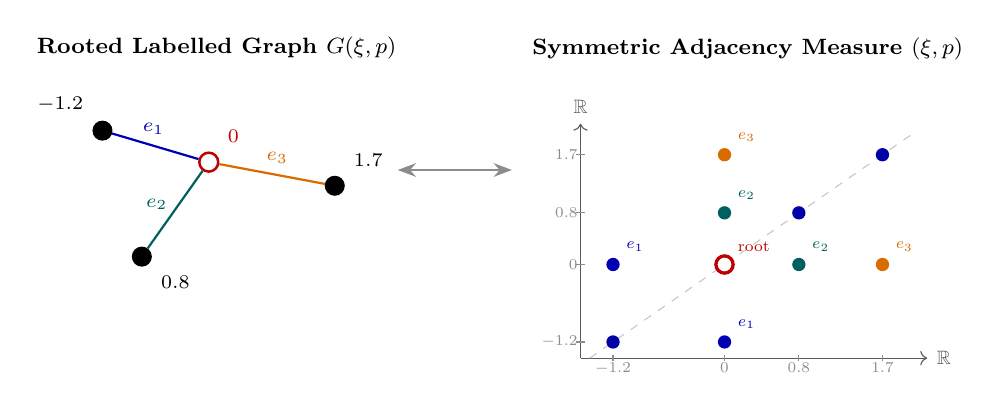
\begin{tikzpicture}[
    font=\scriptsize,
    vertex/.style={circle,draw=black,fill=black,minimum size=2.4mm,inner sep=0pt},
    root/.style={vertex,draw=red!75!black,fill=white,line width=0.9pt},
    atom/.style={circle,fill=blue!65!black,inner sep=1.7pt},
    root atom/.style={circle,draw=red!75!black,very thick,fill=white,inner sep=2.2pt},
    atom label/.style={anchor=south west,xshift=2pt,yshift=2pt,scale=0.80}
]
    % Rooted graph with real-valued vertex labels.
    \node[font=\footnotesize\bfseries] at (1.65,2.90) {Rooted Labelled Graph $G(\xi,p)$};

    \node[vertex] (a) at (0.20,1.85) {};
    \node[root]   (r) at (1.55,1.45) {};
    \node[vertex] (b) at (0.70,0.25) {};
    \node[vertex] (c) at (3.15,1.15) {};
    \node[anchor=south east] at ($(a)+(-0.12,0.12)$) {$-1.2$};
    \node[anchor=south west,text=red!75!black] at ($(r)+(0.12,0.12)$) {$0$};
    \node[anchor=north west] at ($(b)+(0.12,-0.12)$) {$0.8$};
    \node[anchor=south west] at ($(c)+(0.12,0.12)$) {$1.7$};

    \draw[blue!70!black,thick] (r) --
        node[pos=0.52,above=3pt,fill=white,inner sep=0.8pt,text=blue!70!black] {$e_1$} (a);
    \draw[teal!75!black,thick] (r) --
        node[pos=0.43,left=3pt,fill=white,inner sep=0.8pt,text=teal!75!black] {$e_2$} (b);
    \draw[orange!85!black,thick] (r) --
        node[pos=0.55,above=3pt,fill=white,inner sep=0.8pt,text=orange!85!black] {$e_3$} (c);

    \draw[<->,>=Stealth,thick,black!45] (3.95,1.35) -- (5.40,1.35);

    % Symmetric adjacency measure: diagonal atoms encode vertices and
    % reflected off-diagonal pairs encode undirected edges.
    \begin{scope}[shift={(8.10,0.15)},x=1.18cm,y=0.82cm]
        \node[font=\footnotesize\bfseries] at (0.25,3.34) {Symmetric Adjacency Measure $(\xi, p)$};

        \draw[->,black!65] (-1.55,-1.45) -- (2.18,-1.45) node[right] {$\mathbb{R}$};
        \draw[->,black!65] (-1.55,-1.45) -- (-1.55,2.18) node[above] {$\mathbb{R}$};
        \draw[dashed,black!22] (-1.45,-1.45) -- (2.05,2.05);

        \foreach \t/\lab in {-1.2/{-1.2},0/0,0.8/{0.8},1.7/{1.7}} {
            \draw[black!45] (\t,-1.50) -- (\t,-1.40) node[below,scale=0.78] {$\lab$};
            \draw[black!45] (-1.60,\t) -- (-1.50,\t) node[left,scale=0.78] {$\lab$};
        }

        \foreach \t in {-1.2,0.8,1.7} \node[atom] at (\t,\t) {};
        \node[root atom] at (0,0) {};
        \node[atom label,text=red!75!black] at (0,0) {root};

        \foreach \x/\y in {-1.2/0,0/-1.2}
            \node[circle,fill=blue!70!black,inner sep=1.7pt] at (\x,\y) {};
        \foreach \x/\y in {0/0.8,0.8/0}
            \node[circle,fill=teal!75!black,inner sep=1.7pt] at (\x,\y) {};
        \foreach \x/\y in {0/1.7,1.7/0}
            \node[circle,fill=orange!85!black,inner sep=1.7pt] at (\x,\y) {};

        \node[atom label,text=blue!70!black] at (-1.2,0) {$e_1$};
        \node[atom label,text=blue!70!black] at (0,-1.2) {$e_1$};
        \node[atom label,text=teal!75!black] at (0,0.8) {$e_2$};
        \node[atom label,text=teal!75!black] at (0.8,0) {$e_2$};
        \node[atom label,text=orange!85!black] at (0,1.7) {$e_3$};
        \node[atom label,text=orange!85!black] at (1.7,0) {$e_3$};
    \end{scope}
\end{tikzpicture}

\begin{itemize}
    \item Can convergence of these point processes $\xi_n \Rightarrow \xi_\infty$ be lifted to local weak convergence of the corresponding graphs $G(\xi_n, U_n) \Rightarrow (G_\infty, p_\infty)$?  
\end{itemize}

\end{frame}

% --------------------------------------------------
\begin{frame}{Constructing Adjacency Processes}
Recall SIRGs:
\begin{itemize}
    \item Constructed from a \textit{collection of vertices} a proper metric space $\mathbb{X}$;
    \item Each pair connected with an isometric connection rule $\kappa(d_\mathbb{X}(x,y), w_x, w_y)$. 
\end{itemize}

\pause 

\vspace{0.4em}

To make our adjacency process $\xi$ represent a SIRG:
\begin{itemize}
    \item Formalize this collection of vertices as a point process $\Gamma$ on $\mathbb{X}$;
    \item Turn $\kappa$ into a measurable kernel $C$ mapping to point processes on $\mathbb{X}^2$;
    \item Then $\xi \sim C(\Gamma)$ is the adjacency process.
\end{itemize}

\pause

\vspace{0.4em}

If this $C$ is nice* and continuous-ish*, we can leverage 
$$
    \Gamma_n \Rightarrow \Gamma_\infty \qquad \Longrightarrow \qquad \xi_n \Rightarrow \xi_\infty
$$
where $\xi_n \sim C(\Gamma_n), \xi_\infty \sim C(\Gamma_\infty)$

\end{frame}

% --------------------------------------------------
\begin{frame}{The Classical Case - Binomial in $\mathbb{R}^d$}
\begin{columns}[T,onlytextwidth]
    \begin{column}{0.52\textwidth}

        If
        \begin{itemize}
            \item $\Gamma_n = \sum_{i=1}^{n}\delta_{X_i}$ with
            $X_i \overset{\mathrm{i.i.d.}}{\sim} \operatorname{Unif}(\mathbb{T}^d_n)$,
            \item $C$ uses a SIRG rule $\kappa\!\left(\lVert x-y\rVert,w_x,w_y\right)$,
            \item $\kappa(t, \cdot, \cdot) \propto t^{-\alpha}$, where $\alpha>d$,
        \end{itemize}
        then
        $$
            G(\xi_n,U_n) \Rightarrow G(\xi_\infty,0),
        $$
        where $\xi_n \sim C(\Gamma_n)$, $\xi_\infty \sim C(\Gamma_\infty)$.
    
        \vspace{0.35cm}

        \textcolor{red}{Note also that $\Gamma^0_n \Rightarrow \Gamma_\infty...$}
        
        \vspace{0.35cm}

        Seems like Palm distribution $\sim$ uniform root choice.
    \end{column}
    \begin{column}{0.44\textwidth}
        \centering
        \resizebox{0.88\linewidth}{!}{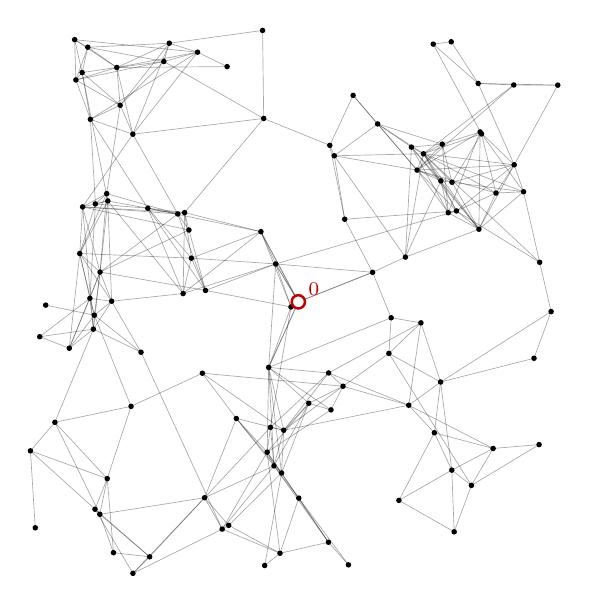
\begin{tikzpicture}[x=0.583333cm, y=0.583333cm]
% Generated by scripts/generate_sirg.py: seed=42, vertices=109, process=poisson(intensity=0.7), line width=0.24pt, opacity=0.34

% Vertices
\coordinate (v0) at (4.303175,2.3684163);
\coordinate (v1) at (-4.8698718,5.7074682);
\coordinate (v2) at (3.1336764,3.4327717);
\coordinate (v3) at (-4.4626364,-0.59536875);
\coordinate (v4) at (-1.5504237,5.1211799);
\coordinate (v5) at (1.7263814,3.8731394);
\coordinate (v6) at (-0.67902961,-3.2731353);
\coordinate (v7) at (0.65501744,-5.2341929);
\coordinate (v8) at (3.9315741,1.5799728);
\coordinate (v9) at (3.0970529,-1.7456884);
\coordinate (v10) at (5.6483763,4.7174535);
\coordinate (v11) at (3.340602,-3.6643355);
\coordinate (v12) at (-0.39934796,-5.4743548);
\coordinate (v13) at (-4.1485261,2.1965874);
\coordinate (v14) at (2.9371459,5.6101168);
\coordinate (v15) at (-2.0900957,-1.5544835);
\coordinate (v16) at (-0.36533026,-3.7263437);
\coordinate (v17) at (-4.4409419,-0.29154089);
\coordinate (v18) at (-3.2770878,2.0377679);
\coordinate (v19) at (-0.75417697,3.9921384);
\coordinate (v20) at (2.4031812,-2.2516003);
\coordinate (v21) at (3.9871176,3.6571723);
\coordinate (v22) at (-1.3502595,-2.5400628);
\coordinate (v23) at (2.189946,-4.3229702);
\coordinate (v24) at (-3.6011016,-5.9116528);
\coordinate (v25) at (3.4430925,1.9782103);
\coordinate (v26) at (2.4619845,3.3687484);
\coordinate (v27) at (-0.49301069,0.82489435);
\coordinate (v28) at (-4.322436,-4.6256391);
\coordinate (v29) at (2.0208355,-0.34684553);
\coordinate (v30) at (0.78283328,3.1799863);
\coordinate (v31) at (1.6166198,0.64295281);
\coordinate (v32) at (0.71048593,-2.3525988);
\coordinate (v33) at (-5.630186,-0.75939133);
\coordinate (v34) at (-3.4249839,-1.0976563);
\coordinate (v35) at (4.2408369,-3.1927262);
\coordinate (v36) at (-5.3003671,-2.6233933);
\coordinate (v37) at (-2.4768749,1.9429982);
\coordinate (v38) at (0.68438583,3.4067785);
\coordinate (v39) at (1.9717625,-1.1233577);
\coordinate (v40) at (3.7682446,-3.996325);
\coordinate (v41) at (-5.7274551,-4.9194257);
\coordinate (v42) at (2.6683122,-0.45747324);
\coordinate (v43) at (-4.0647387,0.012537301);
\coordinate (v44) at (-4.1722548,2.3558445);
\coordinate (v45) at (-0.64612469,-1.4277453);
\coordinate (v46) at (-2.3818549,1.5633911);
\coordinate (v47) at (-1.6582487,-4.948201);
\coordinate (v48) at (-4.5839292,5.542772);
\coordinate (v49) at (4.9029683,2.3964856);
\coordinate (v50) at (-2.8095605,5.6301165);
\coordinate (v51) at (3.3450108,2.6026823);
\coordinate (v52) at (-0.60766197,-2.7331013);
\coordinate (v53) at (-4.8433085,4.8312288);
\coordinate (v54) at (-0.53068452,-3.5716396);
\coordinate (v55) at (-2.3285205,0.95063483);
\coordinate (v56) at (-3.8787266,4.2793714);
\coordinate (v57) at (3.1022344,2.6335555);
\coordinate (v58) at (-0.81488352,1.5277061);
\coordinate (v59) at (1.0091756,1.7981592);
\coordinate (v60) at (-4.9866681,-1.0103112);
\coordinate (v61) at (-5.5006299,-0.072110169);
\coordinate (v62) at (-2.0416655,-4.2657097);
\coordinate (v63) at (-4.7591644,1.0517349);
\coordinate (v64) at (-3.9528844,5.1014414);
\coordinate (v65) at (0.97273368,-1.8375623);
\coordinate (v66) at (1.0909859,-5.7263535);
\coordinate (v67) at (5.5027106,-0.21235876);
\coordinate (v68) at (3.3928227,-5.00724);
\coordinate (v69) at (-0.16010003,-0.11151607);
\coordinate (v70) at (5.2539175,0.86073663);
\coordinate (v71) at (-0.31812719,-2.796292);
\coordinate (v72) at (-2.021172,0.24806883);
\coordinate (v73) at (-0.73306248,-5.740655);
\coordinate (v74) at (3.9155031,4.7539293);
\coordinate (v75) at (-4.3170109,0.64843372);
\coordinate (v76) at (-4.6970911,2.0668811);
\coordinate (v77) at (-2.6251946,1.9130716);
\coordinate (v78) at (2.7239354,3.2237699);
\coordinate (v79) at (-4.7071086,4.9921421);
\coordinate (v80) at (-3.2374321,-5.5510493);
\coordinate (v81) at (0.65822963,-1.5489326);
\coordinate (v82) at (3.9574769,3.6990177);
\coordinate (v83) at (-2.1943333,5.4347927);
\coordinate (v84) at (-2.5089859,0.18068555);
\coordinate (v85) at (-2.9284189,5.2325228);
\coordinate (v86) at (-4.0247062,-5.4610726);
\coordinate (v87) at (-0.77883528,5.9085068);
\coordinate (v88) at (4.7001272,2.9832962);
\coordinate (v89) at (4.6895099,4.7213597);
\coordinate (v90) at (0.22630032,-2.2088514);
\coordinate (v91) at (3.2641492,1.9399352);
\coordinate (v92) at (-1.5161073,-4.8664);
\coordinate (v93) at (2.9614753,-2.8504738);
\coordinate (v94) at (5.2417578,-3.1083531);
\coordinate (v95) at (-4.5269048,3.9733521);
\coordinate (v96) at (-4.1605882,-3.8487803);
\coordinate (v97) at (1.1925935,4.4947445);
\coordinate (v98) at (-3.642784,-2.2761159);
\coordinate (v99) at (3.3288581,5.6619171);
\coordinate (v100) at (0.0088942344,-4.27323);
\coordinate (v101) at (-5.8327645,-3.2441276);
\coordinate (v102) at (-4.4181334,2.1319041);
\coordinate (v103) at (-4.5380099,0.075959179);
\coordinate (v104) at (2.3311492,0.97339931);
\coordinate (v105) at (-3.6026922,3.6494943);
\coordinate (v106) at (2.5848856,2.867808);
\coordinate (v107) at (-4.427307,-4.5149544);
\coordinate (v108) at (5.1307506,-1.2290617);
\coordinate (root) at (0,0);

% Edges
\draw[line width=0.32pt, opacity=0.48] (root) -- (v27);
\draw[line width=0.32pt, opacity=0.48] (root) -- (v31);
\draw[line width=0.32pt, opacity=0.48] (root) -- (v45);
\draw[line width=0.32pt, opacity=0.48] (root) -- (v58);
\draw[line width=0.32pt, opacity=0.48] (root) -- (v69);
\draw[line width=0.24pt, opacity=0.34] (v0) -- (v8);
\draw[line width=0.24pt, opacity=0.34] (v0) -- (v21);
\draw[line width=0.24pt, opacity=0.34] (v0) -- (v25);
\draw[line width=0.24pt, opacity=0.34] (v0) -- (v49);
\draw[line width=0.24pt, opacity=0.34] (v0) -- (v78);
\draw[line width=0.24pt, opacity=0.34] (v0) -- (v88);
\draw[line width=0.24pt, opacity=0.34] (v0) -- (v106);
\draw[line width=0.24pt, opacity=0.34] (v1) -- (v48);
\draw[line width=0.24pt, opacity=0.34] (v1) -- (v53);
\draw[line width=0.24pt, opacity=0.34] (v1) -- (v64);
\draw[line width=0.24pt, opacity=0.34] (v1) -- (v79);
\draw[line width=0.24pt, opacity=0.34] (v1) -- (v83);
\draw[line width=0.24pt, opacity=0.34] (v2) -- (v5);
\draw[line width=0.24pt, opacity=0.34] (v2) -- (v26);
\draw[line width=0.24pt, opacity=0.34] (v2) -- (v51);
\draw[line width=0.24pt, opacity=0.34] (v2) -- (v78);
\draw[line width=0.24pt, opacity=0.34] (v2) -- (v82);
\draw[line width=0.24pt, opacity=0.34] (v2) -- (v91);
\draw[line width=0.24pt, opacity=0.34] (v2) -- (v106);
\draw[line width=0.24pt, opacity=0.34] (v3) -- (v17);
\draw[line width=0.24pt, opacity=0.34] (v3) -- (v33);
\draw[line width=0.24pt, opacity=0.34] (v3) -- (v34);
\draw[line width=0.24pt, opacity=0.34] (v3) -- (v36);
\draw[line width=0.24pt, opacity=0.34] (v3) -- (v43);
\draw[line width=0.24pt, opacity=0.34] (v3) -- (v60);
\draw[line width=0.24pt, opacity=0.34] (v3) -- (v75);
\draw[line width=0.24pt, opacity=0.34] (v3) -- (v76);
\draw[line width=0.24pt, opacity=0.34] (v3) -- (v103);
\draw[line width=0.24pt, opacity=0.34] (v4) -- (v64);
\draw[line width=0.24pt, opacity=0.34] (v4) -- (v83);
\draw[line width=0.24pt, opacity=0.34] (v5) -- (v26);
\draw[line width=0.24pt, opacity=0.34] (v5) -- (v30);
\draw[line width=0.24pt, opacity=0.34] (v5) -- (v78);
\draw[line width=0.24pt, opacity=0.34] (v5) -- (v97);
\draw[line width=0.24pt, opacity=0.34] (v5) -- (v106);
\draw[line width=0.24pt, opacity=0.34] (v6) -- (v7);
\draw[line width=0.24pt, opacity=0.34] (v6) -- (v12);
\draw[line width=0.24pt, opacity=0.34] (v6) -- (v16);
\draw[line width=0.24pt, opacity=0.34] (v6) -- (v22);
\draw[line width=0.24pt, opacity=0.34] (v6) -- (v32);
\draw[line width=0.24pt, opacity=0.34] (v6) -- (v45);
\draw[line width=0.24pt, opacity=0.34] (v6) -- (v47);
\draw[line width=0.24pt, opacity=0.34] (v6) -- (v52);
\draw[line width=0.24pt, opacity=0.34] (v6) -- (v54);
\draw[line width=0.24pt, opacity=0.34] (v6) -- (v90);
\draw[line width=0.24pt, opacity=0.34] (v7) -- (v12);
\draw[line width=0.24pt, opacity=0.34] (v7) -- (v54);
\draw[line width=0.24pt, opacity=0.34] (v7) -- (v66);
\draw[line width=0.24pt, opacity=0.34] (v7) -- (v100);
\draw[line width=0.24pt, opacity=0.34] (v8) -- (v25);
\draw[line width=0.24pt, opacity=0.34] (v8) -- (v26);
\draw[line width=0.24pt, opacity=0.34] (v8) -- (v49);
\draw[line width=0.24pt, opacity=0.34] (v8) -- (v51);
\draw[line width=0.24pt, opacity=0.34] (v8) -- (v57);
\draw[line width=0.24pt, opacity=0.34] (v8) -- (v78);
\draw[line width=0.24pt, opacity=0.34] (v8) -- (v82);
\draw[line width=0.24pt, opacity=0.34] (v8) -- (v88);
\draw[line width=0.24pt, opacity=0.34] (v8) -- (v91);
\draw[line width=0.24pt, opacity=0.34] (v8) -- (v104);
\draw[line width=0.24pt, opacity=0.34] (v9) -- (v11);
\draw[line width=0.24pt, opacity=0.34] (v9) -- (v20);
\draw[line width=0.24pt, opacity=0.34] (v9) -- (v39);
\draw[line width=0.24pt, opacity=0.34] (v9) -- (v42);
\draw[line width=0.24pt, opacity=0.34] (v9) -- (v67);
\draw[line width=0.24pt, opacity=0.34] (v9) -- (v93);
\draw[line width=0.24pt, opacity=0.34] (v9) -- (v108);
\draw[line width=0.24pt, opacity=0.34] (v10) -- (v74);
\draw[line width=0.24pt, opacity=0.34] (v10) -- (v88);
\draw[line width=0.24pt, opacity=0.34] (v10) -- (v89);
\draw[line width=0.24pt, opacity=0.34] (v11) -- (v23);
\draw[line width=0.24pt, opacity=0.34] (v11) -- (v35);
\draw[line width=0.24pt, opacity=0.34] (v11) -- (v40);
\draw[line width=0.24pt, opacity=0.34] (v11) -- (v68);
\draw[line width=0.24pt, opacity=0.34] (v11) -- (v93);
\draw[line width=0.24pt, opacity=0.34] (v12) -- (v47);
\draw[line width=0.24pt, opacity=0.34] (v12) -- (v73);
\draw[line width=0.24pt, opacity=0.34] (v12) -- (v92);
\draw[line width=0.24pt, opacity=0.34] (v12) -- (v100);
\draw[line width=0.24pt, opacity=0.34] (v13) -- (v18);
\draw[line width=0.24pt, opacity=0.34] (v13) -- (v43);
\draw[line width=0.24pt, opacity=0.34] (v13) -- (v44);
\draw[line width=0.24pt, opacity=0.34] (v13) -- (v63);
\draw[line width=0.24pt, opacity=0.34] (v13) -- (v75);
\draw[line width=0.24pt, opacity=0.34] (v13) -- (v76);
\draw[line width=0.24pt, opacity=0.34] (v13) -- (v79);
\draw[line width=0.24pt, opacity=0.34] (v13) -- (v84);
\draw[line width=0.24pt, opacity=0.34] (v13) -- (v102);
\draw[line width=0.24pt, opacity=0.34] (v14) -- (v21);
\draw[line width=0.24pt, opacity=0.34] (v14) -- (v74);
\draw[line width=0.24pt, opacity=0.34] (v14) -- (v99);
\draw[line width=0.24pt, opacity=0.34] (v15) -- (v22);
\draw[line width=0.24pt, opacity=0.34] (v15) -- (v65);
\draw[line width=0.24pt, opacity=0.34] (v15) -- (v71);
\draw[line width=0.24pt, opacity=0.34] (v15) -- (v98);
\draw[line width=0.24pt, opacity=0.34] (v16) -- (v22);
\draw[line width=0.24pt, opacity=0.34] (v16) -- (v45);
\draw[line width=0.24pt, opacity=0.34] (v16) -- (v54);
\draw[line width=0.24pt, opacity=0.34] (v16) -- (v71);
\draw[line width=0.24pt, opacity=0.34] (v16) -- (v73);
\draw[line width=0.24pt, opacity=0.34] (v16) -- (v90);
\draw[line width=0.24pt, opacity=0.34] (v16) -- (v92);
\draw[line width=0.24pt, opacity=0.34] (v16) -- (v100);
\draw[line width=0.24pt, opacity=0.34] (v17) -- (v34);
\draw[line width=0.24pt, opacity=0.34] (v17) -- (v43);
\draw[line width=0.24pt, opacity=0.34] (v17) -- (v60);
\draw[line width=0.24pt, opacity=0.34] (v17) -- (v61);
\draw[line width=0.24pt, opacity=0.34] (v17) -- (v63);
\draw[line width=0.24pt, opacity=0.34] (v17) -- (v75);
\draw[line width=0.24pt, opacity=0.34] (v17) -- (v98);
\draw[line width=0.24pt, opacity=0.34] (v17) -- (v103);
\draw[line width=0.24pt, opacity=0.34] (v18) -- (v37);
\draw[line width=0.24pt, opacity=0.34] (v18) -- (v55);
\draw[line width=0.24pt, opacity=0.34] (v18) -- (v58);
\draw[line width=0.24pt, opacity=0.34] (v18) -- (v72);
\draw[line width=0.24pt, opacity=0.34] (v18) -- (v77);
\draw[line width=0.24pt, opacity=0.34] (v18) -- (v84);
\draw[line width=0.24pt, opacity=0.34] (v18) -- (v95);
\draw[line width=0.24pt, opacity=0.34] (v18) -- (v102);
\draw[line width=0.24pt, opacity=0.34] (v19) -- (v37);
\draw[line width=0.24pt, opacity=0.34] (v19) -- (v38);
\draw[line width=0.24pt, opacity=0.34] (v19) -- (v85);
\draw[line width=0.24pt, opacity=0.34] (v19) -- (v87);
\draw[line width=0.24pt, opacity=0.34] (v19) -- (v105);
\draw[line width=0.24pt, opacity=0.34] (v20) -- (v35);
\draw[line width=0.24pt, opacity=0.34] (v20) -- (v42);
\draw[line width=0.24pt, opacity=0.34] (v20) -- (v65);
\draw[line width=0.24pt, opacity=0.34] (v20) -- (v71);
\draw[line width=0.24pt, opacity=0.34] (v20) -- (v81);
\draw[line width=0.24pt, opacity=0.34] (v20) -- (v93);
\draw[line width=0.24pt, opacity=0.34] (v21) -- (v51);
\draw[line width=0.24pt, opacity=0.34] (v21) -- (v78);
\draw[line width=0.24pt, opacity=0.34] (v21) -- (v82);
\draw[line width=0.24pt, opacity=0.34] (v22) -- (v54);
\draw[line width=0.24pt, opacity=0.34] (v22) -- (v62);
\draw[line width=0.24pt, opacity=0.34] (v22) -- (v71);
\draw[line width=0.24pt, opacity=0.34] (v23) -- (v68);
\draw[line width=0.24pt, opacity=0.34] (v23) -- (v93);
\draw[line width=0.24pt, opacity=0.34] (v24) -- (v47);
\draw[line width=0.24pt, opacity=0.34] (v24) -- (v62);
\draw[line width=0.24pt, opacity=0.34] (v24) -- (v80);
\draw[line width=0.24pt, opacity=0.34] (v24) -- (v107);
\draw[line width=0.24pt, opacity=0.34] (v25) -- (v27);
\draw[line width=0.24pt, opacity=0.34] (v25) -- (v57);
\draw[line width=0.24pt, opacity=0.34] (v25) -- (v59);
\draw[line width=0.24pt, opacity=0.34] (v25) -- (v70);
\draw[line width=0.24pt, opacity=0.34] (v25) -- (v78);
\draw[line width=0.24pt, opacity=0.34] (v25) -- (v88);
\draw[line width=0.24pt, opacity=0.34] (v25) -- (v91);
\draw[line width=0.24pt, opacity=0.34] (v25) -- (v106);
\draw[line width=0.24pt, opacity=0.34] (v26) -- (v57);
\draw[line width=0.24pt, opacity=0.34] (v26) -- (v78);
\draw[line width=0.24pt, opacity=0.34] (v26) -- (v91);
\draw[line width=0.24pt, opacity=0.34] (v26) -- (v104);
\draw[line width=0.24pt, opacity=0.34] (v27) -- (v31);
\draw[line width=0.24pt, opacity=0.34] (v27) -- (v45);
\draw[line width=0.24pt, opacity=0.34] (v27) -- (v55);
\draw[line width=0.24pt, opacity=0.34] (v27) -- (v58);
\draw[line width=0.24pt, opacity=0.34] (v27) -- (v69);
\draw[line width=0.24pt, opacity=0.34] (v27) -- (v72);
\draw[line width=0.24pt, opacity=0.34] (v27) -- (v84);
\draw[line width=0.24pt, opacity=0.34] (v28) -- (v36);
\draw[line width=0.24pt, opacity=0.34] (v28) -- (v62);
\draw[line width=0.24pt, opacity=0.34] (v28) -- (v80);
\draw[line width=0.24pt, opacity=0.34] (v28) -- (v86);
\draw[line width=0.24pt, opacity=0.34] (v28) -- (v96);
\draw[line width=0.24pt, opacity=0.34] (v28) -- (v107);
\draw[line width=0.24pt, opacity=0.34] (v29) -- (v31);
\draw[line width=0.24pt, opacity=0.34] (v29) -- (v39);
\draw[line width=0.24pt, opacity=0.34] (v29) -- (v42);
\draw[line width=0.24pt, opacity=0.34] (v29) -- (v45);
\draw[line width=0.24pt, opacity=0.34] (v30) -- (v38);
\draw[line width=0.24pt, opacity=0.34] (v30) -- (v59);
\draw[line width=0.24pt, opacity=0.34] (v30) -- (v78);
\draw[line width=0.24pt, opacity=0.34] (v30) -- (v104);
\draw[line width=0.24pt, opacity=0.34] (v30) -- (v106);
\draw[line width=0.24pt, opacity=0.34] (v31) -- (v59);
\draw[line width=0.24pt, opacity=0.34] (v31) -- (v104);
\draw[line width=0.24pt, opacity=0.34] (v32) -- (v45);
\draw[line width=0.24pt, opacity=0.34] (v32) -- (v65);
\draw[line width=0.24pt, opacity=0.34] (v32) -- (v90);
\draw[line width=0.24pt, opacity=0.34] (v33) -- (v60);
\draw[line width=0.24pt, opacity=0.34] (v33) -- (v103);
\draw[line width=0.24pt, opacity=0.34] (v34) -- (v43);
\draw[line width=0.24pt, opacity=0.34] (v34) -- (v47);
\draw[line width=0.24pt, opacity=0.34] (v35) -- (v40);
\draw[line width=0.24pt, opacity=0.34] (v35) -- (v93);
\draw[line width=0.24pt, opacity=0.34] (v35) -- (v94);
\draw[line width=0.24pt, opacity=0.34] (v36) -- (v96);
\draw[line width=0.24pt, opacity=0.34] (v36) -- (v98);
\draw[line width=0.24pt, opacity=0.34] (v36) -- (v101);
\draw[line width=0.24pt, opacity=0.34] (v37) -- (v46);
\draw[line width=0.24pt, opacity=0.34] (v37) -- (v55);
\draw[line width=0.24pt, opacity=0.34] (v37) -- (v58);
\draw[line width=0.24pt, opacity=0.34] (v37) -- (v76);
\draw[line width=0.24pt, opacity=0.34] (v37) -- (v77);
\draw[line width=0.24pt, opacity=0.34] (v37) -- (v84);
\draw[line width=0.24pt, opacity=0.34] (v38) -- (v59);
\draw[line width=0.24pt, opacity=0.34] (v38) -- (v97);
\draw[line width=0.24pt, opacity=0.34] (v39) -- (v40);
\draw[line width=0.24pt, opacity=0.34] (v39) -- (v42);
\draw[line width=0.24pt, opacity=0.34] (v39) -- (v65);
\draw[line width=0.24pt, opacity=0.34] (v40) -- (v68);
\draw[line width=0.24pt, opacity=0.34] (v40) -- (v94);
\draw[line width=0.24pt, opacity=0.34] (v41) -- (v101);
\draw[line width=0.24pt, opacity=0.34] (v42) -- (v81);
\draw[line width=0.24pt, opacity=0.34] (v43) -- (v63);
\draw[line width=0.24pt, opacity=0.34] (v43) -- (v75);
\draw[line width=0.24pt, opacity=0.34] (v43) -- (v84);
\draw[line width=0.24pt, opacity=0.34] (v43) -- (v103);
\draw[line width=0.24pt, opacity=0.34] (v44) -- (v56);
\draw[line width=0.24pt, opacity=0.34] (v44) -- (v63);
\draw[line width=0.24pt, opacity=0.34] (v44) -- (v75);
\draw[line width=0.24pt, opacity=0.34] (v44) -- (v76);
\draw[line width=0.24pt, opacity=0.34] (v44) -- (v77);
\draw[line width=0.24pt, opacity=0.34] (v44) -- (v102);
\draw[line width=0.24pt, opacity=0.34] (v45) -- (v54);
\draw[line width=0.24pt, opacity=0.34] (v45) -- (v69);
\draw[line width=0.24pt, opacity=0.34] (v45) -- (v71);
\draw[line width=0.24pt, opacity=0.34] (v45) -- (v81);
\draw[line width=0.24pt, opacity=0.34] (v45) -- (v90);
\draw[line width=0.24pt, opacity=0.34] (v46) -- (v72);
\draw[line width=0.24pt, opacity=0.34] (v46) -- (v75);
\draw[line width=0.24pt, opacity=0.34] (v46) -- (v76);
\draw[line width=0.24pt, opacity=0.34] (v46) -- (v77);
\draw[line width=0.24pt, opacity=0.34] (v47) -- (v54);
\draw[line width=0.24pt, opacity=0.34] (v47) -- (v62);
\draw[line width=0.24pt, opacity=0.34] (v47) -- (v92);
\draw[line width=0.24pt, opacity=0.34] (v48) -- (v50);
\draw[line width=0.24pt, opacity=0.34] (v48) -- (v53);
\draw[line width=0.24pt, opacity=0.34] (v48) -- (v64);
\draw[line width=0.24pt, opacity=0.34] (v48) -- (v79);
\draw[line width=0.24pt, opacity=0.34] (v48) -- (v85);
\draw[line width=0.24pt, opacity=0.34] (v49) -- (v51);
\draw[line width=0.24pt, opacity=0.34] (v49) -- (v70);
\draw[line width=0.24pt, opacity=0.34] (v49) -- (v78);
\draw[line width=0.24pt, opacity=0.34] (v49) -- (v82);
\draw[line width=0.24pt, opacity=0.34] (v49) -- (v88);
\draw[line width=0.24pt, opacity=0.34] (v50) -- (v56);
\draw[line width=0.24pt, opacity=0.34] (v50) -- (v64);
\draw[line width=0.24pt, opacity=0.34] (v50) -- (v83);
\draw[line width=0.24pt, opacity=0.34] (v50) -- (v85);
\draw[line width=0.24pt, opacity=0.34] (v50) -- (v87);
\draw[line width=0.24pt, opacity=0.34] (v50) -- (v105);
\draw[line width=0.24pt, opacity=0.34] (v51) -- (v57);
\draw[line width=0.24pt, opacity=0.34] (v51) -- (v78);
\draw[line width=0.24pt, opacity=0.34] (v51) -- (v88);
\draw[line width=0.24pt, opacity=0.34] (v51) -- (v106);
\draw[line width=0.24pt, opacity=0.34] (v52) -- (v54);
\draw[line width=0.24pt, opacity=0.34] (v52) -- (v62);
\draw[line width=0.24pt, opacity=0.34] (v52) -- (v69);
\draw[line width=0.24pt, opacity=0.34] (v52) -- (v71);
\draw[line width=0.24pt, opacity=0.34] (v52) -- (v81);
\draw[line width=0.24pt, opacity=0.34] (v53) -- (v56);
\draw[line width=0.24pt, opacity=0.34] (v53) -- (v64);
\draw[line width=0.24pt, opacity=0.34] (v53) -- (v79);
\draw[line width=0.24pt, opacity=0.34] (v53) -- (v85);
\draw[line width=0.24pt, opacity=0.34] (v53) -- (v95);
\draw[line width=0.24pt, opacity=0.34] (v54) -- (v62);
\draw[line width=0.24pt, opacity=0.34] (v54) -- (v71);
\draw[line width=0.24pt, opacity=0.34] (v54) -- (v90);
\draw[line width=0.24pt, opacity=0.34] (v54) -- (v100);
\draw[line width=0.24pt, opacity=0.34] (v55) -- (v58);
\draw[line width=0.24pt, opacity=0.34] (v55) -- (v63);
\draw[line width=0.24pt, opacity=0.34] (v55) -- (v72);
\draw[line width=0.24pt, opacity=0.34] (v55) -- (v84);
\draw[line width=0.24pt, opacity=0.34] (v56) -- (v64);
\draw[line width=0.24pt, opacity=0.34] (v56) -- (v79);
\draw[line width=0.24pt, opacity=0.34] (v56) -- (v85);
\draw[line width=0.24pt, opacity=0.34] (v56) -- (v95);
\draw[line width=0.24pt, opacity=0.34] (v56) -- (v105);
\draw[line width=0.24pt, opacity=0.34] (v57) -- (v78);
\draw[line width=0.24pt, opacity=0.34] (v57) -- (v91);
\draw[line width=0.24pt, opacity=0.34] (v57) -- (v104);
\draw[line width=0.24pt, opacity=0.34] (v57) -- (v106);
\draw[line width=0.24pt, opacity=0.34] (v58) -- (v69);
\draw[line width=0.24pt, opacity=0.34] (v58) -- (v84);
\draw[line width=0.24pt, opacity=0.34] (v60) -- (v63);
\draw[line width=0.24pt, opacity=0.34] (v60) -- (v75);
\draw[line width=0.24pt, opacity=0.34] (v60) -- (v103);
\draw[line width=0.24pt, opacity=0.34] (v62) -- (v80);
\draw[line width=0.24pt, opacity=0.34] (v62) -- (v92);
\draw[line width=0.24pt, opacity=0.34] (v63) -- (v75);
\draw[line width=0.24pt, opacity=0.34] (v63) -- (v76);
\draw[line width=0.24pt, opacity=0.34] (v63) -- (v102);
\draw[line width=0.24pt, opacity=0.34] (v63) -- (v103);
\draw[line width=0.24pt, opacity=0.34] (v64) -- (v79);
\draw[line width=0.24pt, opacity=0.34] (v64) -- (v83);
\draw[line width=0.24pt, opacity=0.34] (v64) -- (v85);
\draw[line width=0.24pt, opacity=0.34] (v64) -- (v105);
\draw[line width=0.24pt, opacity=0.34] (v65) -- (v71);
\draw[line width=0.24pt, opacity=0.34] (v65) -- (v81);
\draw[line width=0.24pt, opacity=0.34] (v65) -- (v90);
\draw[line width=0.24pt, opacity=0.34] (v66) -- (v100);
\draw[line width=0.24pt, opacity=0.34] (v67) -- (v70);
\draw[line width=0.24pt, opacity=0.34] (v67) -- (v108);
\draw[line width=0.24pt, opacity=0.34] (v69) -- (v72);
\draw[line width=0.24pt, opacity=0.34] (v70) -- (v78);
\draw[line width=0.24pt, opacity=0.34] (v71) -- (v81);
\draw[line width=0.24pt, opacity=0.34] (v71) -- (v90);
\draw[line width=0.24pt, opacity=0.34] (v72) -- (v75);
\draw[line width=0.24pt, opacity=0.34] (v72) -- (v77);
\draw[line width=0.24pt, opacity=0.34] (v74) -- (v88);
\draw[line width=0.24pt, opacity=0.34] (v74) -- (v89);
\draw[line width=0.24pt, opacity=0.34] (v74) -- (v99);
\draw[line width=0.24pt, opacity=0.34] (v75) -- (v76);
\draw[line width=0.24pt, opacity=0.34] (v75) -- (v77);
\draw[line width=0.24pt, opacity=0.34] (v75) -- (v103);
\draw[line width=0.24pt, opacity=0.34] (v76) -- (v77);
\draw[line width=0.24pt, opacity=0.34] (v76) -- (v105);
\draw[line width=0.24pt, opacity=0.34] (v77) -- (v105);
\draw[line width=0.24pt, opacity=0.34] (v78) -- (v88);
\draw[line width=0.24pt, opacity=0.34] (v78) -- (v89);
\draw[line width=0.24pt, opacity=0.34] (v78) -- (v104);
\draw[line width=0.24pt, opacity=0.34] (v78) -- (v106);
\draw[line width=0.24pt, opacity=0.34] (v79) -- (v95);
\draw[line width=0.24pt, opacity=0.34] (v80) -- (v86);
\draw[line width=0.24pt, opacity=0.34] (v80) -- (v107);
\draw[line width=0.24pt, opacity=0.34] (v82) -- (v88);
\draw[line width=0.24pt, opacity=0.34] (v82) -- (v91);
\draw[line width=0.24pt, opacity=0.34] (v82) -- (v106);
\draw[line width=0.24pt, opacity=0.34] (v83) -- (v85);
\draw[line width=0.24pt, opacity=0.34] (v83) -- (v95);
\draw[line width=0.24pt, opacity=0.34] (v83) -- (v105);
\draw[line width=0.24pt, opacity=0.34] (v86) -- (v96);
\draw[line width=0.24pt, opacity=0.34] (v88) -- (v106);
\draw[line width=0.24pt, opacity=0.34] (v89) -- (v106);
\draw[line width=0.24pt, opacity=0.34] (v91) -- (v106);
\draw[line width=0.24pt, opacity=0.34] (v95) -- (v102);
\draw[line width=0.24pt, opacity=0.34] (v95) -- (v105);
\draw[line width=0.24pt, opacity=0.34] (v96) -- (v98);
\draw[line width=0.24pt, opacity=0.34] (v96) -- (v101);
\draw[line width=0.24pt, opacity=0.34] (v96) -- (v107);
\draw[line width=0.24pt, opacity=0.34] (v97) -- (v106);
\draw[line width=0.24pt, opacity=0.34] (v101) -- (v107);
\draw[line width=0.24pt, opacity=0.34] (v102) -- (v103);

% Vertices
\foreach \v in {v0,v1,v2,v3,v4,v5,v6,v7,v8,v9,v10,v11,v12,v13,v14,v15,v16,v17,v18,v19,v20,v21,v22,v23,v24,v25,v26,v27,v28,v29,v30,v31,v32,v33,v34,v35,v36,v37,v38,v39,v40,v41,v42,v43,v44,v45,v46,v47,v48,v49,v50,v51,v52,v53,v54,v55,v56,v57,v58,v59,v60,v61,v62,v63,v64,v65,v66,v67,v68,v69,v70,v71,v72,v73,v74,v75,v76,v77,v78,v79,v80,v81,v82,v83,v84,v85,v86,v87,v88,v89,v90,v91,v92,v93,v94,v95,v96,v97,v98,v99,v100,v101,v102,v103,v104,v105,v106,v107,v108} {
    \fill (\v) circle (1pt);
}
\fill[white] (root) circle (2.4pt);
\draw[red!75!black,line width=0.9pt] (root) circle (2.4pt);
\node[red!75!black,anchor=south west,inner sep=0pt,xshift=3.4pt,yshift=2.2pt,font=\scriptsize] at (root) {$0$};
\end{tikzpicture}
}
        \par\vspace{0.12cm}
        \textbf{Poisson SIRG limit}
        \par\vspace{0.06cm}
        $\Gamma_\infty \overset{d}{=} \operatorname{PPP}(1)+\delta_0$
    \end{column}
\end{columns}
\end{frame}

% --------------------------------------------------
\begin{frame}{The Main Theorem}
Consider a sequence of finite stationary \textit{vertex} processes $(\Gamma_n)_{n \in \mathbb{N}}$, placed along a $\text{nice}^*$ compact exhaustion of a proper metric space $\mathbb{X}$, and let $C$ be a $\text{nice}^*$, continuous-ish, isometric connection rule (measurable SIRG kernel). Suppose that
\begin{enumerate}
    \item $\Gamma_n^{o} \Rightarrow \Gamma_\infty$; 
    \item The vertices concentrate via 
    $$\frac{|\Gamma_n|}{\mathbb{E}|\Gamma_n|}\overset{L^1}{\longrightarrow} 1;$$
    \item $(\xi_n, o)_{n \in \mathbb{N}} \sim C(\Gamma_n^{o}, \cdot)$ is \textit{radially} $\textit{tight}^*$.
\end{enumerate}
Then, the corresponding graphs converge locally weakly, $$G(\xi_n, U_n) \Rightarrow G(\xi_\infty, o),$$ where $\xi_\infty \sim C(\Gamma_\infty, \cdot)$. 
\end{frame}

% --------------------------------------------------
\begin{frame}{Novel Results - More Vertex Processes}
\begin{columns}[T,onlytextwidth]
    \begin{column}{0.50\textwidth}
        Sticking with $\mathbb{R}^d$ and $\mathbb{T}^d_n$ for now, we can handle:
        \begin{itemize}
            \item Mixed-Binomial vertex processes $\sum_{n=0}^N \delta_{U_i}$
            \item Cox vertex processes (Phase-Shifted, \textcolor{red}{Shot-Noise, Lévy})
            \item \textcolor{red}{Neyman-Scott / Clustering}
            \item \textcolor{red}{Bernoulli Site processes (for atomic spaces)}
        \end{itemize}
    \end{column}
    \begin{column}{0.46\textwidth}
        \centering
        \resizebox{\linewidth}{!}{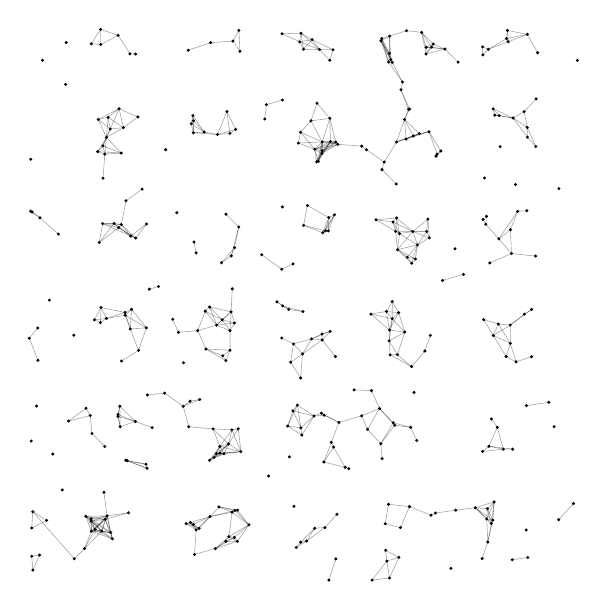
\begin{tikzpicture}[x=0.35cm, y=0.35cm]
% Generated by scripts/generate_sirg.py: seed=random, vertices=393, process=cox(period=3.6, phase=(0.809155,2.11685)), line width=0.22pt, opacity=0.35

% Vertices
\coordinate (v0) at (1.504373,-5.8919327);
\coordinate (v1) at (3.9145074,-2.2384569);
\coordinate (v2) at (-7.4709543,5.5612234);
\coordinate (v3) at (-4.0060302,-7.9652251);
\coordinate (v4) at (3.2495782,-4.2782285);
\coordinate (v5) at (3.452296,-9.1617038);
\coordinate (v6) at (-2.7264908,-5.0428301);
\coordinate (v7) at (-0.96883496,0.11095678);
\coordinate (v8) at (-3.2074367,-8.8417513);
\coordinate (v9) at (6.8647213,-7.8099776);
\coordinate (v10) at (8.27228,-0.16266839);
\coordinate (v11) at (3.4012828,-1.8063898);
\coordinate (v12) at (-6.0960412,2.4258187);
\coordinate (v13) at (-6.4442899,3.7789518);
\coordinate (v14) at (-4.0027992,6.2462091);
\coordinate (v15) at (-7.7133008,-7.7588092);
\coordinate (v16) at (3.2138451,0.12635315);
\coordinate (v17) at (-2.9548592,-0.54239383);
\coordinate (v18) at (-8.5313328,-4.2146127);
\coordinate (v19) at (1.0649463,9.2564667);
\coordinate (v20) at (-5.9915255,-1.64975);
\coordinate (v21) at (9.7879021,-7.2090746);
\coordinate (v22) at (-7.3264546,-8.2074643);
\coordinate (v23) at (0.89609259,2.6851213);
\coordinate (v24) at (-7.2796973,4.5948322);
\coordinate (v25) at (6.9342059,6.8847502);
\coordinate (v26) at (-3.2522128,-5.5355874);
\coordinate (v27) at (7.9998786,7.013242);
\coordinate (v28) at (1.1184394,3.2733619);
\coordinate (v29) at (-0.11702542,6.2639087);
\coordinate (v30) at (-0.067313901,-4.7227234);
\coordinate (v31) at (-2.3752493,-4.4978925);
\coordinate (v32) at (2.8024545,9.577104);
\coordinate (v33) at (4.1034115,-4.9205692);
\coordinate (v34) at (3.3057237,-4.3650615);
\coordinate (v35) at (-4.6037194,3.3453104);
\coordinate (v36) at (6.9108067,-7.1468809);
\coordinate (v37) at (4.5468324,6.2848836);
\coordinate (v38) at (6.5613521,4.604721);
\coordinate (v39) at (-6.94236,-8.4860146);
\coordinate (v40) at (-7.1576274,-0.49255642);
\coordinate (v41) at (-8.9006972,2.570014);
\coordinate (v42) at (6.6994289,9.2747416);
\coordinate (v43) at (-6.2441685,-0.16045558);
\coordinate (v44) at (-0.38443486,1.486675);
\coordinate (v45) at (0.74464399,-4.0026148);
\coordinate (v46) at (6.4761605,-9.2036588);
\coordinate (v47) at (4.1273001,2.1776781);
\coordinate (v48) at (-7.8973929,-3.7506084);
\coordinate (v49) at (7.0802434,2.3969233);
\coordinate (v50) at (7.566525,-9.2479993);
\coordinate (v51) at (4.8009645,5.3982197);
\coordinate (v52) at (-3.9025764,-8.1644589);
\coordinate (v53) at (6.6348334,3.2134865);
\coordinate (v54) at (1.1658684,-9.2162469);
\coordinate (v55) at (6.6431444,-7.7696326);
\coordinate (v56) at (-7.1567043,6.0796009);
\coordinate (v57) at (-6.4514173,-5.6369995);
\coordinate (v58) at (4.7802174,-7.5525962);
\coordinate (v59) at (-6.7368907,-3.9793416);
\coordinate (v60) at (2.1072538,5.7620367);
\coordinate (v61) at (1.2072635,-7.5982049);
\coordinate (v62) at (8.0085034,-0.33664804);
\coordinate (v63) at (-8.7599321,-6.7130414);
\coordinate (v64) at (-2.350227,9.9617064);
\coordinate (v65) at (-7.7459959,-4.0141339);
\coordinate (v66) at (-7.365092,9.4476565);
\coordinate (v67) at (4.1972816,6.2159894);
\coordinate (v68) at (0.67550926,5.913652);
\coordinate (v69) at (-3.6095119,6.2698219);
\coordinate (v70) at (-1.9863683,-7.9797372);
\coordinate (v71) at (7.762455,3.39247);
\coordinate (v72) at (9.9284179,8.8728784);
\coordinate (v73) at (-6.8795896,2.9561779);
\coordinate (v74) at (-2.980281,1.5307366);
\coordinate (v75) at (-9.1012823,-5.4122758);
\coordinate (v76) at (-3.0363482,-5.3817358);
\coordinate (v77) at (-2.4055172,-8.5778881);
\coordinate (v78) at (0.3980482,-8.1051673);
\coordinate (v79) at (8.1114796,6.4403626);
\coordinate (v80) at (-6.54368,6.4309986);
\coordinate (v81) at (-6.7398342,-4.0477161);
\coordinate (v82) at (-0.04210936,-1.7782419);
\coordinate (v83) at (-0.23076119,-3.6360913);
\coordinate (v84) at (3.8400939,-7.3185296);
\coordinate (v85) at (-2.6740047,-1.6435196);
\coordinate (v86) at (3.3730801,3.1554264);
\coordinate (v87) at (-3.1266189,6.1834663);
\coordinate (v88) at (8.423556,5.747786);
\coordinate (v89) at (5.7981333,1.1063394);
\coordinate (v90) at (-3.546872,-1.6025221);
\coordinate (v91) at (-0.14516434,9.5452097);
\coordinate (v92) at (-5.4991105,-4.4557706);
\coordinate (v93) at (1.2802477,-4.2641453);
\coordinate (v94) at (-7.0957089,6.8061263);
\coordinate (v95) at (-6.6174209,2.9154542);
\coordinate (v96) at (-6.302618,9.1102575);
\coordinate (v97) at (-7.903861,-7.6707955);
\coordinate (v98) at (-9.8666628,-9.1178397);
\coordinate (v99) at (-2.8221824,-2.0241988);
\coordinate (v100) at (-2.5092284,-0.65487602);
\coordinate (v101) at (0.40179326,5.6490243);
\coordinate (v102) at (-0.57920971,-4.3971942);
\coordinate (v103) at (-6.1066501,-4.2309197);
\coordinate (v104) at (-4.1095483,-7.8935374);
\coordinate (v105) at (0.48116521,7.3167833);
\coordinate (v106) at (2.8427419,4.9083335);
\coordinate (v107) at (-9.8265799,-9.6211404);
\coordinate (v108) at (8.0750906,-8.1655478);
\coordinate (v109) at (-7.2184978,-5.1352905);
\coordinate (v110) at (-7.3750784,-0.64274143);
\coordinate (v111) at (3.2393328,3.0092845);
\coordinate (v112) at (-6.732327,9.7797393);
\coordinate (v113) at (2.9764225,-8.9040896);
\coordinate (v114) at (3.1616853,8.8975889);
\coordinate (v115) at (8.0797725,-3.6552065);
\coordinate (v116) at (-2.6757773,6.223821);
\coordinate (v117) at (-8.6161539,9.5167941);
\coordinate (v118) at (-2.88785,-5.398476);
\coordinate (v119) at (-0.794493,-1.2011994);
\coordinate (v120) at (6.8762931,7.1134918);
\coordinate (v121) at (-6.4809412,-0.27300287);
\coordinate (v122) at (-7.284715,5.7702918);
\coordinate (v123) at (7.7047244,-2.0662625);
\coordinate (v124) at (-0.35380411,-7.3068075);
\coordinate (v125) at (1.0040075,-4.9843527);
\coordinate (v126) at (-6.6567872,-4.4192482);
\coordinate (v127) at (7.063272,-0.69511304);
\coordinate (v128) at (-9.8669182,-8.0971883);
\coordinate (v129) at (-3.8448472,-0.93264014);
\coordinate (v130) at (1.636797,-5.9416135);
\coordinate (v131) at (-3.9598826,-9.0555319);
\coordinate (v132) at (-3.0420297,-5.1357274);
\coordinate (v133) at (-6.2752157,2.4966299);
\coordinate (v134) at (8.4885737,9.1492602);
\coordinate (v135) at (3.9602705,2.6637768);
\coordinate (v136) at (-9.8288461,-7.5030215);
\coordinate (v137) at (-7.7041082,9.4743099);
\coordinate (v138) at (5.5145691,-7.4500297);
\coordinate (v139) at (-9.3258423,-7.8176612);
\coordinate (v140) at (0.37643631,-4.0312153);
\coordinate (v141) at (-0.11000161,-8.6112431);
\coordinate (v142) at (7.5405182,1.862832);
\coordinate (v143) at (3.135184,-1.8127058);
\coordinate (v144) at (3.0753941,-7.2358049);
\coordinate (v145) at (-5.6004766,0.57085745);
\coordinate (v146) at (9.2535475,-7.7923475);
\coordinate (v147) at (6.6063883,2.9269569);
\coordinate (v148) at (0.68977211,2.6173926);
\coordinate (v149) at (5.3428746,-9.5587322);
\coordinate (v150) at (3.5848671,8.0881927);
\coordinate (v151) at (-3.9787892,2.2796573);
\coordinate (v152) at (0.13736478,3.6078707);
\coordinate (v153) at (0.97076122,5.9284487);
\coordinate (v154) at (3.510136,-8.0787664);
\coordinate (v155) at (-0.53912455,-0.16352718);
\coordinate (v156) at (1.8295279,-3.0854273);
\coordinate (v157) at (-3.0744571,-7.3300034);
\coordinate (v158) at (-3.7947094,-8.1128606);
\coordinate (v159) at (3.5291276,7.8057081);
\coordinate (v160) at (-3.4122541,-0.075781212);
\coordinate (v161) at (2.8472334,-5.5785761);
\coordinate (v162) at (-7.5929343,-0.53923849);
\coordinate (v163) at (2.9588007,-7.9407777);
\coordinate (v164) at (-2.820331,3.291285);
\coordinate (v165) at (-0.11114362,-2.6518247);
\coordinate (v166) at (3.4057566,2.0040757);
\coordinate (v167) at (-2.7862619,7.0159002);
\coordinate (v168) at (-4.750498,-0.52093803);
\coordinate (v169) at (-6.4039029,-5.6537828);
\coordinate (v170) at (7.0919382,6.8693036);
\coordinate (v171) at (-1.3532422,7.2689505);
\coordinate (v172) at (3.7168025,6.018114);
\coordinate (v173) at (-6.6072141,-2.0353772);
\coordinate (v174) at (0.77008895,-8.0778329);
\coordinate (v175) at (-9.5699139,3.1608118);
\coordinate (v176) at (-7.134579,-7.6555183);
\coordinate (v177) at (7.5013068,2.7271867);
\coordinate (v178) at (0.64393054,-3.9307534);
\coordinate (v179) at (-0.76722631,7.4341528);
\coordinate (v180) at (4.8436697,5.470858);
\coordinate (v181) at (0.26376323,6.6792526);
\coordinate (v182) at (-1.5218937,1.8205612);
\coordinate (v183) at (-0.47200213,-2.0805172);
\coordinate (v184) at (3.6594387,6.7278276);
\coordinate (v185) at (6.6669609,-7.3946268);
\coordinate (v186) at (3.1017383,-1.3034639);
\coordinate (v187) at (-3.1595673,-0.73262898);
\coordinate (v188) at (3.3363259,2.6696073);
\coordinate (v189) at (-7.0013079,-8.2614);
\coordinate (v190) at (-3.7746056,-3.4330233);
\coordinate (v191) at (-7.7126832,-7.8483506);
\coordinate (v192) at (-4.5426783,-0.99535038);
\coordinate (v193) at (-2.4944984,-7.4581848);
\coordinate (v194) at (8.0955185,3.4203476);
\coordinate (v195) at (7.0254582,-4.4411311);
\coordinate (v196) at (8.2688482,-1.8791128);
\coordinate (v197) at (-8.3217412,-9.2107556);
\coordinate (v198) at (6.5106979,3.09979);
\coordinate (v199) at (3.3580396,4.3875759);
\coordinate (v200) at (7.129522,5.7434599);
\coordinate (v201) at (-4.1696966,-4.4205012);
\coordinate (v202) at (3.7298806,9.9494628);
\coordinate (v203) at (-8.6393429,8.0003025);
\coordinate (v204) at (-3.399295,-7.6814377);
\coordinate (v205) at (-7.3539913,-0.096667322);
\coordinate (v206) at (2.7981169,-5.0371254);
\coordinate (v207) at (-2.7143062,-8.4079256);
\coordinate (v208) at (0.57260359,9.2670437);
\coordinate (v209) at (-7.4180394,2.2632033);
\coordinate (v210) at (1.2377413,5.8267697);
\coordinate (v211) at (2.4391072,-0.33384515);
\coordinate (v212) at (-2.4009721,-7.4479385);
\coordinate (v213) at (7.6007812,6.7818453);
\coordinate (v214) at (-2.6742753,-0.93351569);
\coordinate (v215) at (-3.375132,9.5130283);
\coordinate (v216) at (3.2170269,8.7968347);
\coordinate (v217) at (-9.2260766,0.17125118);
\coordinate (v218) at (-6.6980013,7.1193438);
\coordinate (v219) at (5.1247881,9.2835302);
\coordinate (v220) at (6.7202572,-5.1298264);
\coordinate (v221) at (0.6631145,-1.054832);
\coordinate (v222) at (-0.098001893,9.8580598);
\coordinate (v223) at (0.53130963,5.2070332);
\coordinate (v224) at (-9.6487224,-0.83636209);
\coordinate (v225) at (-0.027590603,-0.24078925);
\coordinate (v226) at (-6.0148231,6.8190345);
\coordinate (v227) at (4.977568,5.5839009);
\coordinate (v228) at (-9.6420398,-2.0118526);
\coordinate (v229) at (-5.6704579,-3.2679155);
\coordinate (v230) at (2.752682,-3.7612823);
\coordinate (v231) at (-2.3576905,2.8262087);
\coordinate (v232) at (-4.3716211,-3.6796823);
\coordinate (v233) at (7.4999858,-1.3947325);
\coordinate (v234) at (-0.51781731,-5.5132417);
\coordinate (v235) at (4.057896,1.6648847);
\coordinate (v236) at (1.1635501,5.9111416);
\coordinate (v237) at (0.9132957,-9.9872555);
\coordinate (v238) at (3.0038609,-0.23747575);
\coordinate (v239) at (6.5322098,-0.5355929);
\coordinate (v240) at (3.8426655,7.1027811);
\coordinate (v241) at (2.6273234,3.0869119);
\coordinate (v242) at (-2.2766926,-5.3248095);
\coordinate (v243) at (-2.5652013,9.5726068);
\coordinate (v244) at (-0.0066780279,9.2760325);
\coordinate (v245) at (-4.2649812,-7.9341873);
\coordinate (v246) at (7.6876097,4.3687647);
\coordinate (v247) at (-9.9052723,3.4017623);
\coordinate (v248) at (-2.508078,2.0776165);
\coordinate (v249) at (0.30466804,9.6243217);
\coordinate (v250) at (-5.0089592,5.6290444);
\coordinate (v251) at (8.4128505,1.7722067);
\coordinate (v252) at (3.8046018,7.0968905);
\coordinate (v253) at (-5.6830367,-5.9293291);
\coordinate (v254) at (-7.5714074,-8.1493831);
\coordinate (v255) at (8.1149563,9.8152101);
\coordinate (v256) at (-2.5134177,-8.4357009);
\coordinate (v257) at (-7.2001837,-7.7792964);
\coordinate (v258) at (6.8803629,-1.1124287);
\coordinate (v259) at (-1.4112894,6.7442948);
\coordinate (v260) at (-0.77171122,3.5543968);
\coordinate (v261) at (-6.3544446,-7.5423633);
\coordinate (v262) at (0.96135031,-0.95929016);
\coordinate (v263) at (-9.9032599,5.2853212);
\coordinate (v264) at (-5.0446768,-3.2009144);
\coordinate (v265) at (-2.4668371,6.3685612);
\coordinate (v266) at (9.2619772,4.2196754);
\coordinate (v267) at (-0.19266119,5.8724328);
\coordinate (v268) at (-7.293809,2.9488659);
\coordinate (v269) at (-2.6329401,-0.24970706);
\coordinate (v270) at (3.9210642,1.5119757);
\coordinate (v271) at (-7.950815,-8.8399013);
\coordinate (v272) at (-4.1895524,9.2408716);
\coordinate (v273) at (0.73361998,-5.7003521);
\coordinate (v274) at (2.317345,-4.513861);
\coordinate (v275) at (-7.2467575,-6.8000157);
\coordinate (v276) at (-0.78485515,9.8395901);
\coordinate (v277) at (5.6021805,8.8102531);
\coordinate (v278) at (3.8822381,-4.4399474);
\coordinate (v279) at (0.47145607,5.1891783);
\coordinate (v280) at (7.5856589,-5.2342933);
\coordinate (v281) at (-2.6270679,1.7790135);
\coordinate (v282) at (7.2432546,-5.2353303);
\coordinate (v283) at (3.4753058,2.5865778);
\coordinate (v284) at (-3.8995505,1.8873222);
\coordinate (v285) at (-4.0190619,6.8709936);
\coordinate (v286) at (3.1126277,-9.9076527);
\coordinate (v287) at (-2.8270867,-8.5791155);
\coordinate (v288) at (4.3969963,-1.6728617);
\coordinate (v289) at (2.1038162,-4.0225963);
\coordinate (v290) at (-7.4527324,6.7299381);
\coordinate (v291) at (-7.7060219,-8.2113255);
\coordinate (v292) at (-3.5707978,-0.22644913);
\coordinate (v293) at (3.0183421,-9.2953453);
\coordinate (v294) at (3.3684992,5.9129895);
\coordinate (v295) at (-2.5920216,0.58091873);
\coordinate (v296) at (-1.274948,-6.210781);
\coordinate (v297) at (8.4345357,7.4730787);
\coordinate (v298) at (-5.2647599,0.667271);
\coordinate (v299) at (7.3602234,9.6623175);
\coordinate (v300) at (-0.0018019136,2.888303);
\coordinate (v301) at (2.4818426,-9.9869527);
\coordinate (v302) at (-4.0802907,6.571462);
\coordinate (v303) at (-9.853103,3.3712074);
\coordinate (v304) at (-5.7211966,-5.7810293);
\coordinate (v305) at (-4.1207422,-3.4948597);
\coordinate (v306) at (3.4461913,-0.28353193);
\coordinate (v307) at (-2.936531,-1.8470972);
\coordinate (v308) at (-9.4769498,8.8753195);
\coordinate (v309) at (-2.5972421,-7.5218483);
\coordinate (v310) at (-2.3134113,9.201022);
\coordinate (v311) at (7.4196607,9.548934);
\coordinate (v312) at (1.1503424,-1.8729707);
\coordinate (v313) at (3.7591445,1.7272657);
\coordinate (v314) at (4.6433183,9.3518124);
\coordinate (v315) at (0.91180492,3.1684552);
\coordinate (v316) at (-6.6221693,5.5103019);
\coordinate (v317) at (4.6999388,9.465213);
\coordinate (v318) at (8.8927679,-3.5357925);
\coordinate (v319) at (-0.766081,-0.035571572);
\coordinate (v320) at (-8.3424699,-1.0980452);
\coordinate (v321) at (-5.8628435,4.2011063);
\coordinate (v322) at (0.28691664,-1.2328417);
\coordinate (v323) at (5.0413203,0.88642183);
\coordinate (v324) at (1.0847437,-5.158242);
\coordinate (v325) at (-0.39052629,-3.8466565);
\coordinate (v326) at (-6.6699146,-3.6764132);
\coordinate (v327) at (-3.1689312,-5.3963467);
\coordinate (v328) at (9.089445,-4.4175416);
\coordinate (v329) at (0.67170815,-1.2714645);
\coordinate (v330) at (6.4928292,9.3633874);
\coordinate (v331) at (0.67250188,5.5969139);
\coordinate (v332) at (4.6217058,-7.6309559);
\coordinate (v333) at (0.94591888,8.8750797);
\coordinate (v334) at (-0.79534717,1.294448);
\coordinate (v335) at (6.2276322,-7.3610166);
\coordinate (v336) at (6.4934073,-5.3176414);
\coordinate (v337) at (-6.4761045,-0.37333525);
\coordinate (v338) at (-5.7086618,-0.83085973);
\coordinate (v339) at (3.2156575,-0.50198898);
\coordinate (v340) at (-9.8855824,-4.9361501);
\coordinate (v341) at (2.2810008,5.6305148);
\coordinate (v342) at (7.3948195,9.9589645);
\coordinate (v343) at (0.10659609,-8.5684423);
\coordinate (v344) at (-2.6029912,-4.5339163);
\coordinate (v345) at (0.79019014,2.6883956);
\coordinate (v346) at (4.0043445,-3.1756855);
\coordinate (v347) at (4.5968108,-1.1081666);
\coordinate (v348) at (3.1110072,-0.91066274);
\coordinate (v349) at (6.8130828,-4.1370515);
\coordinate (v350) at (-7.3691906,9.9989411);
\coordinate (v351) at (-3.2870759,-4.4997459);
\coordinate (v352) at (3.0784083,8.816125);
\coordinate (v353) at (8.1188488,6.0866204);
\coordinate (v354) at (4.4447113,9.3470949);
\coordinate (v355) at (-9.692501,-3.6706032);
\coordinate (v356) at (5.489626,2.039362);
\coordinate (v357) at (-9.5839019,-9.0787346);
\coordinate (v358) at (-0.10033489,-4.4612168);
\coordinate (v359) at (6.8092811,-7.931906);
\coordinate (v360) at (-6.2913595,-0.87329558);
\coordinate (v361) at (2.8323598,9.6625399);
\coordinate (v362) at (3.9771718,6.1317445);
\coordinate (v363) at (3.1164737,9.7522454);
\coordinate (v364) at (0.94762441,6.7685295);
\coordinate (v365) at (6.5003211,9.0722104);
\coordinate (v366) at (-7.2159515,5.4678764);
\coordinate (v367) at (-6.098837,9.1029647);
\coordinate (v368) at (4.4621141,2.6646932);
\coordinate (v369) at (7.3460261,-1.8727195);
\coordinate (v370) at (-3.417059,-5.6351139);
\coordinate (v371) at (3.1121573,9.1273005);
\coordinate (v372) at (7.4962147,-0.72966938);
\coordinate (v373) at (4.5054527,3.1114012);
\coordinate (v374) at (2.4598425,-3.1104357);
\coordinate (v375) at (4.4396627,9.1050408);
\coordinate (v376) at (3.6666476,-0.98672733);
\coordinate (v377) at (-6.7129137,2.8060846);
\coordinate (v378) at (6.6815653,-8.6050807);
\coordinate (v379) at (-5.7011406,2.9351855);
\coordinate (v380) at (-7.0173139,6.383616);
\coordinate (v381) at (-9.9545083,-1.2101153);
\coordinate (v382) at (-4.3575353,-2.0989283);
\coordinate (v383) at (-7.6801172,-4.663923);
\coordinate (v384) at (4.5606773,2.4338698);
\coordinate (v385) at (8.1318831,-9.1647644);
\coordinate (v386) at (4.2795177,9.8886189);
\coordinate (v387) at (-3.998811,6.6831824);
\coordinate (v388) at (-0.26850111,-8.8021112);
\coordinate (v389) at (6.7534089,1.5239016);
\coordinate (v390) at (-0.36947027,-1.4157657);
\coordinate (v391) at (2.9219625,5.1826458);
\coordinate (v392) at (0.65904577,5.4914889);

% Edges
\draw[line width=0.22pt, opacity=0.35] (v0) -- (v130);
\draw[line width=0.22pt, opacity=0.35] (v0) -- (v273);
\draw[line width=0.22pt, opacity=0.35] (v0) -- (v324);
\draw[line width=0.22pt, opacity=0.35] (v1) -- (v11);
\draw[line width=0.22pt, opacity=0.35] (v1) -- (v143);
\draw[line width=0.22pt, opacity=0.35] (v1) -- (v288);
\draw[line width=0.22pt, opacity=0.35] (v2) -- (v56);
\draw[line width=0.22pt, opacity=0.35] (v2) -- (v122);
\draw[line width=0.22pt, opacity=0.35] (v2) -- (v316);
\draw[line width=0.22pt, opacity=0.35] (v2) -- (v366);
\draw[line width=0.22pt, opacity=0.35] (v3) -- (v52);
\draw[line width=0.22pt, opacity=0.35] (v3) -- (v104);
\draw[line width=0.22pt, opacity=0.35] (v3) -- (v158);
\draw[line width=0.22pt, opacity=0.35] (v3) -- (v204);
\draw[line width=0.22pt, opacity=0.35] (v3) -- (v245);
\draw[line width=0.22pt, opacity=0.35] (v4) -- (v34);
\draw[line width=0.22pt, opacity=0.35] (v4) -- (v206);
\draw[line width=0.22pt, opacity=0.35] (v4) -- (v230);
\draw[line width=0.22pt, opacity=0.35] (v4) -- (v278);
\draw[line width=0.22pt, opacity=0.35] (v5) -- (v113);
\draw[line width=0.22pt, opacity=0.35] (v5) -- (v286);
\draw[line width=0.22pt, opacity=0.35] (v5) -- (v293);
\draw[line width=0.22pt, opacity=0.35] (v6) -- (v26);
\draw[line width=0.22pt, opacity=0.35] (v6) -- (v31);
\draw[line width=0.22pt, opacity=0.35] (v6) -- (v76);
\draw[line width=0.22pt, opacity=0.35] (v6) -- (v118);
\draw[line width=0.22pt, opacity=0.35] (v6) -- (v132);
\draw[line width=0.22pt, opacity=0.35] (v6) -- (v242);
\draw[line width=0.22pt, opacity=0.35] (v6) -- (v327);
\draw[line width=0.22pt, opacity=0.35] (v6) -- (v344);
\draw[line width=0.22pt, opacity=0.35] (v6) -- (v351);
\draw[line width=0.22pt, opacity=0.35] (v7) -- (v155);
\draw[line width=0.22pt, opacity=0.35] (v7) -- (v319);
\draw[line width=0.22pt, opacity=0.35] (v8) -- (v77);
\draw[line width=0.22pt, opacity=0.35] (v8) -- (v131);
\draw[line width=0.22pt, opacity=0.35] (v8) -- (v207);
\draw[line width=0.22pt, opacity=0.35] (v8) -- (v256);
\draw[line width=0.22pt, opacity=0.35] (v8) -- (v287);
\draw[line width=0.22pt, opacity=0.35] (v9) -- (v36);
\draw[line width=0.22pt, opacity=0.35] (v9) -- (v55);
\draw[line width=0.22pt, opacity=0.35] (v9) -- (v185);
\draw[line width=0.22pt, opacity=0.35] (v9) -- (v335);
\draw[line width=0.22pt, opacity=0.35] (v9) -- (v359);
\draw[line width=0.22pt, opacity=0.35] (v9) -- (v378);
\draw[line width=0.22pt, opacity=0.35] (v10) -- (v62);
\draw[line width=0.22pt, opacity=0.35] (v10) -- (v372);
\draw[line width=0.22pt, opacity=0.35] (v11) -- (v143);
\draw[line width=0.22pt, opacity=0.35] (v11) -- (v186);
\draw[line width=0.22pt, opacity=0.35] (v11) -- (v376);
\draw[line width=0.22pt, opacity=0.35] (v12) -- (v95);
\draw[line width=0.22pt, opacity=0.35] (v12) -- (v133);
\draw[line width=0.22pt, opacity=0.35] (v12) -- (v268);
\draw[line width=0.22pt, opacity=0.35] (v12) -- (v377);
\draw[line width=0.22pt, opacity=0.35] (v12) -- (v379);
\draw[line width=0.22pt, opacity=0.35] (v13) -- (v95);
\draw[line width=0.22pt, opacity=0.35] (v13) -- (v321);
\draw[line width=0.22pt, opacity=0.35] (v14) -- (v69);
\draw[line width=0.22pt, opacity=0.35] (v14) -- (v87);
\draw[line width=0.22pt, opacity=0.35] (v14) -- (v285);
\draw[line width=0.22pt, opacity=0.35] (v14) -- (v302);
\draw[line width=0.22pt, opacity=0.35] (v14) -- (v387);
\draw[line width=0.22pt, opacity=0.35] (v15) -- (v22);
\draw[line width=0.22pt, opacity=0.35] (v15) -- (v97);
\draw[line width=0.22pt, opacity=0.35] (v15) -- (v176);
\draw[line width=0.22pt, opacity=0.35] (v15) -- (v189);
\draw[line width=0.22pt, opacity=0.35] (v15) -- (v191);
\draw[line width=0.22pt, opacity=0.35] (v15) -- (v254);
\draw[line width=0.22pt, opacity=0.35] (v15) -- (v257);
\draw[line width=0.22pt, opacity=0.35] (v15) -- (v291);
\draw[line width=0.22pt, opacity=0.35] (v16) -- (v238);
\draw[line width=0.22pt, opacity=0.35] (v16) -- (v306);
\draw[line width=0.22pt, opacity=0.35] (v16) -- (v339);
\draw[line width=0.22pt, opacity=0.35] (v17) -- (v100);
\draw[line width=0.22pt, opacity=0.35] (v17) -- (v160);
\draw[line width=0.22pt, opacity=0.35] (v17) -- (v187);
\draw[line width=0.22pt, opacity=0.35] (v17) -- (v214);
\draw[line width=0.22pt, opacity=0.35] (v17) -- (v269);
\draw[line width=0.22pt, opacity=0.35] (v17) -- (v292);
\draw[line width=0.22pt, opacity=0.35] (v18) -- (v48);
\draw[line width=0.22pt, opacity=0.35] (v18) -- (v65);
\draw[line width=0.22pt, opacity=0.35] (v19) -- (v208);
\draw[line width=0.22pt, opacity=0.35] (v19) -- (v249);
\draw[line width=0.22pt, opacity=0.35] (v19) -- (v333);
\draw[line width=0.22pt, opacity=0.35] (v20) -- (v173);
\draw[line width=0.22pt, opacity=0.35] (v20) -- (v338);
\draw[line width=0.22pt, opacity=0.35] (v20) -- (v360);
\draw[line width=0.22pt, opacity=0.35] (v21) -- (v146);
\draw[line width=0.22pt, opacity=0.35] (v22) -- (v39);
\draw[line width=0.22pt, opacity=0.35] (v22) -- (v97);
\draw[line width=0.22pt, opacity=0.35] (v22) -- (v176);
\draw[line width=0.22pt, opacity=0.35] (v22) -- (v189);
\draw[line width=0.22pt, opacity=0.35] (v22) -- (v191);
\draw[line width=0.22pt, opacity=0.35] (v22) -- (v254);
\draw[line width=0.22pt, opacity=0.35] (v22) -- (v257);
\draw[line width=0.22pt, opacity=0.35] (v22) -- (v271);
\draw[line width=0.22pt, opacity=0.35] (v22) -- (v291);
\draw[line width=0.22pt, opacity=0.35] (v23) -- (v28);
\draw[line width=0.22pt, opacity=0.35] (v23) -- (v148);
\draw[line width=0.22pt, opacity=0.35] (v23) -- (v315);
\draw[line width=0.22pt, opacity=0.35] (v23) -- (v345);
\draw[line width=0.22pt, opacity=0.35] (v24) -- (v366);
\draw[line width=0.22pt, opacity=0.35] (v25) -- (v120);
\draw[line width=0.22pt, opacity=0.35] (v25) -- (v170);
\draw[line width=0.22pt, opacity=0.35] (v25) -- (v213);
\draw[line width=0.22pt, opacity=0.35] (v26) -- (v76);
\draw[line width=0.22pt, opacity=0.35] (v26) -- (v118);
\draw[line width=0.22pt, opacity=0.35] (v26) -- (v132);
\draw[line width=0.22pt, opacity=0.35] (v26) -- (v327);
\draw[line width=0.22pt, opacity=0.35] (v26) -- (v370);
\draw[line width=0.22pt, opacity=0.35] (v27) -- (v79);
\draw[line width=0.22pt, opacity=0.35] (v27) -- (v213);
\draw[line width=0.22pt, opacity=0.35] (v27) -- (v297);
\draw[line width=0.22pt, opacity=0.35] (v28) -- (v148);
\draw[line width=0.22pt, opacity=0.35] (v28) -- (v315);
\draw[line width=0.22pt, opacity=0.35] (v28) -- (v345);
\draw[line width=0.22pt, opacity=0.35] (v29) -- (v68);
\draw[line width=0.22pt, opacity=0.35] (v29) -- (v101);
\draw[line width=0.22pt, opacity=0.35] (v29) -- (v181);
\draw[line width=0.22pt, opacity=0.35] (v29) -- (v267);
\draw[line width=0.22pt, opacity=0.35] (v30) -- (v102);
\draw[line width=0.22pt, opacity=0.35] (v30) -- (v140);
\draw[line width=0.22pt, opacity=0.35] (v30) -- (v358);
\draw[line width=0.22pt, opacity=0.35] (v31) -- (v242);
\draw[line width=0.22pt, opacity=0.35] (v31) -- (v344);
\draw[line width=0.22pt, opacity=0.35] (v32) -- (v114);
\draw[line width=0.22pt, opacity=0.35] (v32) -- (v216);
\draw[line width=0.22pt, opacity=0.35] (v32) -- (v352);
\draw[line width=0.22pt, opacity=0.35] (v32) -- (v361);
\draw[line width=0.22pt, opacity=0.35] (v32) -- (v363);
\draw[line width=0.22pt, opacity=0.35] (v32) -- (v371);
\draw[line width=0.22pt, opacity=0.35] (v33) -- (v278);
\draw[line width=0.22pt, opacity=0.35] (v34) -- (v206);
\draw[line width=0.22pt, opacity=0.35] (v34) -- (v230);
\draw[line width=0.22pt, opacity=0.35] (v34) -- (v278);
\draw[line width=0.22pt, opacity=0.35] (v36) -- (v55);
\draw[line width=0.22pt, opacity=0.35] (v36) -- (v185);
\draw[line width=0.22pt, opacity=0.35] (v36) -- (v335);
\draw[line width=0.22pt, opacity=0.35] (v36) -- (v359);
\draw[line width=0.22pt, opacity=0.35] (v37) -- (v67);
\draw[line width=0.22pt, opacity=0.35] (v37) -- (v172);
\draw[line width=0.22pt, opacity=0.35] (v37) -- (v180);
\draw[line width=0.22pt, opacity=0.35] (v37) -- (v227);
\draw[line width=0.22pt, opacity=0.35] (v37) -- (v362);
\draw[line width=0.22pt, opacity=0.35] (v39) -- (v176);
\draw[line width=0.22pt, opacity=0.35] (v39) -- (v189);
\draw[line width=0.22pt, opacity=0.35] (v39) -- (v254);
\draw[line width=0.22pt, opacity=0.35] (v39) -- (v257);
\draw[line width=0.22pt, opacity=0.35] (v39) -- (v291);
\draw[line width=0.22pt, opacity=0.35] (v40) -- (v110);
\draw[line width=0.22pt, opacity=0.35] (v40) -- (v121);
\draw[line width=0.22pt, opacity=0.35] (v40) -- (v162);
\draw[line width=0.22pt, opacity=0.35] (v40) -- (v205);
\draw[line width=0.22pt, opacity=0.35] (v40) -- (v337);
\draw[line width=0.22pt, opacity=0.35] (v41) -- (v175);
\draw[line width=0.22pt, opacity=0.35] (v42) -- (v299);
\draw[line width=0.22pt, opacity=0.35] (v42) -- (v311);
\draw[line width=0.22pt, opacity=0.35] (v42) -- (v330);
\draw[line width=0.22pt, opacity=0.35] (v42) -- (v365);
\draw[line width=0.22pt, opacity=0.35] (v43) -- (v121);
\draw[line width=0.22pt, opacity=0.35] (v43) -- (v337);
\draw[line width=0.22pt, opacity=0.35] (v43) -- (v338);
\draw[line width=0.22pt, opacity=0.35] (v43) -- (v360);
\draw[line width=0.22pt, opacity=0.35] (v44) -- (v334);
\draw[line width=0.22pt, opacity=0.35] (v45) -- (v93);
\draw[line width=0.22pt, opacity=0.35] (v45) -- (v140);
\draw[line width=0.22pt, opacity=0.35] (v45) -- (v178);
\draw[line width=0.22pt, opacity=0.35] (v46) -- (v378);
\draw[line width=0.22pt, opacity=0.35] (v47) -- (v135);
\draw[line width=0.22pt, opacity=0.35] (v47) -- (v166);
\draw[line width=0.22pt, opacity=0.35] (v47) -- (v235);
\draw[line width=0.22pt, opacity=0.35] (v47) -- (v270);
\draw[line width=0.22pt, opacity=0.35] (v47) -- (v283);
\draw[line width=0.22pt, opacity=0.35] (v47) -- (v313);
\draw[line width=0.22pt, opacity=0.35] (v47) -- (v368);
\draw[line width=0.22pt, opacity=0.35] (v47) -- (v384);
\draw[line width=0.22pt, opacity=0.35] (v48) -- (v65);
\draw[line width=0.22pt, opacity=0.35] (v49) -- (v71);
\draw[line width=0.22pt, opacity=0.35] (v49) -- (v142);
\draw[line width=0.22pt, opacity=0.35] (v49) -- (v147);
\draw[line width=0.22pt, opacity=0.35] (v49) -- (v177);
\draw[line width=0.22pt, opacity=0.35] (v50) -- (v385);
\draw[line width=0.22pt, opacity=0.35] (v51) -- (v180);
\draw[line width=0.22pt, opacity=0.35] (v51) -- (v227);
\draw[line width=0.22pt, opacity=0.35] (v52) -- (v104);
\draw[line width=0.22pt, opacity=0.35] (v52) -- (v131);
\draw[line width=0.22pt, opacity=0.35] (v52) -- (v158);
\draw[line width=0.22pt, opacity=0.35] (v52) -- (v204);
\draw[line width=0.22pt, opacity=0.35] (v52) -- (v245);
\draw[line width=0.22pt, opacity=0.35] (v53) -- (v147);
\draw[line width=0.22pt, opacity=0.35] (v53) -- (v198);
\draw[line width=0.22pt, opacity=0.35] (v54) -- (v237);
\draw[line width=0.22pt, opacity=0.35] (v55) -- (v185);
\draw[line width=0.22pt, opacity=0.35] (v55) -- (v335);
\draw[line width=0.22pt, opacity=0.35] (v55) -- (v359);
\draw[line width=0.22pt, opacity=0.35] (v55) -- (v378);
\draw[line width=0.22pt, opacity=0.35] (v56) -- (v80);
\draw[line width=0.22pt, opacity=0.35] (v56) -- (v94);
\draw[line width=0.22pt, opacity=0.35] (v56) -- (v122);
\draw[line width=0.22pt, opacity=0.35] (v56) -- (v290);
\draw[line width=0.22pt, opacity=0.35] (v56) -- (v316);
\draw[line width=0.22pt, opacity=0.35] (v56) -- (v366);
\draw[line width=0.22pt, opacity=0.35] (v56) -- (v380);
\draw[line width=0.22pt, opacity=0.35] (v57) -- (v169);
\draw[line width=0.22pt, opacity=0.35] (v57) -- (v253);
\draw[line width=0.22pt, opacity=0.35] (v57) -- (v304);
\draw[line width=0.22pt, opacity=0.35] (v58) -- (v138);
\draw[line width=0.22pt, opacity=0.35] (v58) -- (v332);
\draw[line width=0.22pt, opacity=0.35] (v59) -- (v81);
\draw[line width=0.22pt, opacity=0.35] (v59) -- (v103);
\draw[line width=0.22pt, opacity=0.35] (v59) -- (v126);
\draw[line width=0.22pt, opacity=0.35] (v59) -- (v326);
\draw[line width=0.22pt, opacity=0.35] (v60) -- (v210);
\draw[line width=0.22pt, opacity=0.35] (v60) -- (v341);
\draw[line width=0.22pt, opacity=0.35] (v61) -- (v174);
\draw[line width=0.22pt, opacity=0.35] (v62) -- (v372);
\draw[line width=0.22pt, opacity=0.35] (v64) -- (v243);
\draw[line width=0.22pt, opacity=0.35] (v64) -- (v310);
\draw[line width=0.22pt, opacity=0.35] (v65) -- (v383);
\draw[line width=0.22pt, opacity=0.35] (v66) -- (v112);
\draw[line width=0.22pt, opacity=0.35] (v66) -- (v137);
\draw[line width=0.22pt, opacity=0.35] (v66) -- (v350);
\draw[line width=0.22pt, opacity=0.35] (v67) -- (v172);
\draw[line width=0.22pt, opacity=0.35] (v67) -- (v184);
\draw[line width=0.22pt, opacity=0.35] (v67) -- (v294);
\draw[line width=0.22pt, opacity=0.35] (v67) -- (v362);
\draw[line width=0.22pt, opacity=0.35] (v68) -- (v101);
\draw[line width=0.22pt, opacity=0.35] (v68) -- (v153);
\draw[line width=0.22pt, opacity=0.35] (v68) -- (v181);
\draw[line width=0.22pt, opacity=0.35] (v68) -- (v210);
\draw[line width=0.22pt, opacity=0.35] (v68) -- (v223);
\draw[line width=0.22pt, opacity=0.35] (v68) -- (v236);
\draw[line width=0.22pt, opacity=0.35] (v68) -- (v267);
\draw[line width=0.22pt, opacity=0.35] (v68) -- (v279);
\draw[line width=0.22pt, opacity=0.35] (v68) -- (v331);
\draw[line width=0.22pt, opacity=0.35] (v68) -- (v364);
\draw[line width=0.22pt, opacity=0.35] (v68) -- (v392);
\draw[line width=0.22pt, opacity=0.35] (v69) -- (v87);
\draw[line width=0.22pt, opacity=0.35] (v69) -- (v285);
\draw[line width=0.22pt, opacity=0.35] (v69) -- (v302);
\draw[line width=0.22pt, opacity=0.35] (v69) -- (v387);
\draw[line width=0.22pt, opacity=0.35] (v70) -- (v77);
\draw[line width=0.22pt, opacity=0.35] (v70) -- (v193);
\draw[line width=0.22pt, opacity=0.35] (v70) -- (v207);
\draw[line width=0.22pt, opacity=0.35] (v70) -- (v212);
\draw[line width=0.22pt, opacity=0.35] (v70) -- (v256);
\draw[line width=0.22pt, opacity=0.35] (v70) -- (v309);
\draw[line width=0.22pt, opacity=0.35] (v71) -- (v177);
\draw[line width=0.22pt, opacity=0.35] (v71) -- (v194);
\draw[line width=0.22pt, opacity=0.35] (v73) -- (v95);
\draw[line width=0.22pt, opacity=0.35] (v73) -- (v133);
\draw[line width=0.22pt, opacity=0.35] (v73) -- (v209);
\draw[line width=0.22pt, opacity=0.35] (v73) -- (v268);
\draw[line width=0.22pt, opacity=0.35] (v73) -- (v377);
\draw[line width=0.22pt, opacity=0.35] (v74) -- (v248);
\draw[line width=0.22pt, opacity=0.35] (v74) -- (v281);
\draw[line width=0.22pt, opacity=0.35] (v76) -- (v118);
\draw[line width=0.22pt, opacity=0.35] (v76) -- (v132);
\draw[line width=0.22pt, opacity=0.35] (v76) -- (v242);
\draw[line width=0.22pt, opacity=0.35] (v76) -- (v327);
\draw[line width=0.22pt, opacity=0.35] (v76) -- (v370);
\draw[line width=0.22pt, opacity=0.35] (v77) -- (v207);
\draw[line width=0.22pt, opacity=0.35] (v77) -- (v256);
\draw[line width=0.22pt, opacity=0.35] (v77) -- (v287);
\draw[line width=0.22pt, opacity=0.35] (v78) -- (v141);
\draw[line width=0.22pt, opacity=0.35] (v78) -- (v174);
\draw[line width=0.22pt, opacity=0.35] (v78) -- (v343);
\draw[line width=0.22pt, opacity=0.35] (v79) -- (v88);
\draw[line width=0.22pt, opacity=0.35] (v79) -- (v213);
\draw[line width=0.22pt, opacity=0.35] (v79) -- (v353);
\draw[line width=0.22pt, opacity=0.35] (v80) -- (v94);
\draw[line width=0.22pt, opacity=0.35] (v80) -- (v218);
\draw[line width=0.22pt, opacity=0.35] (v80) -- (v226);
\draw[line width=0.22pt, opacity=0.35] (v80) -- (v380);
\draw[line width=0.22pt, opacity=0.35] (v81) -- (v103);
\draw[line width=0.22pt, opacity=0.35] (v81) -- (v126);
\draw[line width=0.22pt, opacity=0.35] (v81) -- (v326);
\draw[line width=0.22pt, opacity=0.35] (v82) -- (v165);
\draw[line width=0.22pt, opacity=0.35] (v82) -- (v183);
\draw[line width=0.22pt, opacity=0.35] (v82) -- (v322);
\draw[line width=0.22pt, opacity=0.35] (v82) -- (v329);
\draw[line width=0.22pt, opacity=0.35] (v82) -- (v390);
\draw[line width=0.22pt, opacity=0.35] (v83) -- (v102);
\draw[line width=0.22pt, opacity=0.35] (v83) -- (v140);
\draw[line width=0.22pt, opacity=0.35] (v83) -- (v325);
\draw[line width=0.22pt, opacity=0.35] (v83) -- (v358);
\draw[line width=0.22pt, opacity=0.35] (v84) -- (v144);
\draw[line width=0.22pt, opacity=0.35] (v84) -- (v154);
\draw[line width=0.22pt, opacity=0.35] (v84) -- (v332);
\draw[line width=0.22pt, opacity=0.35] (v85) -- (v90);
\draw[line width=0.22pt, opacity=0.35] (v85) -- (v99);
\draw[line width=0.22pt, opacity=0.35] (v85) -- (v214);
\draw[line width=0.22pt, opacity=0.35] (v85) -- (v307);
\draw[line width=0.22pt, opacity=0.35] (v86) -- (v111);
\draw[line width=0.22pt, opacity=0.35] (v86) -- (v135);
\draw[line width=0.22pt, opacity=0.35] (v86) -- (v188);
\draw[line width=0.22pt, opacity=0.35] (v86) -- (v241);
\draw[line width=0.22pt, opacity=0.35] (v86) -- (v283);
\draw[line width=0.22pt, opacity=0.35] (v87) -- (v116);
\draw[line width=0.22pt, opacity=0.35] (v87) -- (v167);
\draw[line width=0.22pt, opacity=0.35] (v87) -- (v265);
\draw[line width=0.22pt, opacity=0.35] (v88) -- (v353);
\draw[line width=0.22pt, opacity=0.35] (v89) -- (v323);
\draw[line width=0.22pt, opacity=0.35] (v90) -- (v99);
\draw[line width=0.22pt, opacity=0.35] (v90) -- (v129);
\draw[line width=0.22pt, opacity=0.35] (v90) -- (v307);
\draw[line width=0.22pt, opacity=0.35] (v91) -- (v208);
\draw[line width=0.22pt, opacity=0.35] (v91) -- (v222);
\draw[line width=0.22pt, opacity=0.35] (v91) -- (v244);
\draw[line width=0.22pt, opacity=0.35] (v91) -- (v249);
\draw[line width=0.22pt, opacity=0.35] (v91) -- (v276);
\draw[line width=0.22pt, opacity=0.35] (v92) -- (v103);
\draw[line width=0.22pt, opacity=0.35] (v93) -- (v125);
\draw[line width=0.22pt, opacity=0.35] (v93) -- (v178);
\draw[line width=0.22pt, opacity=0.35] (v93) -- (v289);
\draw[line width=0.22pt, opacity=0.35] (v94) -- (v218);
\draw[line width=0.22pt, opacity=0.35] (v94) -- (v290);
\draw[line width=0.22pt, opacity=0.35] (v94) -- (v380);
\draw[line width=0.22pt, opacity=0.35] (v95) -- (v133);
\draw[line width=0.22pt, opacity=0.35] (v95) -- (v268);
\draw[line width=0.22pt, opacity=0.35] (v95) -- (v377);
\draw[line width=0.22pt, opacity=0.35] (v96) -- (v112);
\draw[line width=0.22pt, opacity=0.35] (v96) -- (v367);
\draw[line width=0.22pt, opacity=0.35] (v97) -- (v176);
\draw[line width=0.22pt, opacity=0.35] (v97) -- (v191);
\draw[line width=0.22pt, opacity=0.35] (v97) -- (v254);
\draw[line width=0.22pt, opacity=0.35] (v97) -- (v257);
\draw[line width=0.22pt, opacity=0.35] (v97) -- (v291);
\draw[line width=0.22pt, opacity=0.35] (v98) -- (v107);
\draw[line width=0.22pt, opacity=0.35] (v98) -- (v357);
\draw[line width=0.22pt, opacity=0.35] (v99) -- (v307);
\draw[line width=0.22pt, opacity=0.35] (v100) -- (v187);
\draw[line width=0.22pt, opacity=0.35] (v100) -- (v214);
\draw[line width=0.22pt, opacity=0.35] (v100) -- (v269);
\draw[line width=0.22pt, opacity=0.35] (v101) -- (v153);
\draw[line width=0.22pt, opacity=0.35] (v101) -- (v210);
\draw[line width=0.22pt, opacity=0.35] (v101) -- (v223);
\draw[line width=0.22pt, opacity=0.35] (v101) -- (v236);
\draw[line width=0.22pt, opacity=0.35] (v101) -- (v267);
\draw[line width=0.22pt, opacity=0.35] (v101) -- (v279);
\draw[line width=0.22pt, opacity=0.35] (v101) -- (v331);
\draw[line width=0.22pt, opacity=0.35] (v101) -- (v392);
\draw[line width=0.22pt, opacity=0.35] (v102) -- (v325);
\draw[line width=0.22pt, opacity=0.35] (v102) -- (v358);
\draw[line width=0.22pt, opacity=0.35] (v103) -- (v126);
\draw[line width=0.22pt, opacity=0.35] (v103) -- (v326);
\draw[line width=0.22pt, opacity=0.35] (v104) -- (v158);
\draw[line width=0.22pt, opacity=0.35] (v104) -- (v204);
\draw[line width=0.22pt, opacity=0.35] (v104) -- (v245);
\draw[line width=0.22pt, opacity=0.35] (v105) -- (v181);
\draw[line width=0.22pt, opacity=0.35] (v105) -- (v364);
\draw[line width=0.22pt, opacity=0.35] (v106) -- (v199);
\draw[line width=0.22pt, opacity=0.35] (v106) -- (v391);
\draw[line width=0.22pt, opacity=0.35] (v107) -- (v357);
\draw[line width=0.22pt, opacity=0.35] (v109) -- (v383);
\draw[line width=0.22pt, opacity=0.35] (v110) -- (v162);
\draw[line width=0.22pt, opacity=0.35] (v110) -- (v205);
\draw[line width=0.22pt, opacity=0.35] (v111) -- (v135);
\draw[line width=0.22pt, opacity=0.35] (v111) -- (v188);
\draw[line width=0.22pt, opacity=0.35] (v111) -- (v241);
\draw[line width=0.22pt, opacity=0.35] (v111) -- (v283);
\draw[line width=0.22pt, opacity=0.35] (v112) -- (v350);
\draw[line width=0.22pt, opacity=0.35] (v113) -- (v293);
\draw[line width=0.22pt, opacity=0.35] (v114) -- (v216);
\draw[line width=0.22pt, opacity=0.35] (v114) -- (v352);
\draw[line width=0.22pt, opacity=0.35] (v114) -- (v361);
\draw[line width=0.22pt, opacity=0.35] (v114) -- (v363);
\draw[line width=0.22pt, opacity=0.35] (v114) -- (v371);
\draw[line width=0.22pt, opacity=0.35] (v115) -- (v318);
\draw[line width=0.22pt, opacity=0.35] (v116) -- (v167);
\draw[line width=0.22pt, opacity=0.35] (v116) -- (v265);
\draw[line width=0.22pt, opacity=0.35] (v118) -- (v132);
\draw[line width=0.22pt, opacity=0.35] (v118) -- (v242);
\draw[line width=0.22pt, opacity=0.35] (v118) -- (v327);
\draw[line width=0.22pt, opacity=0.35] (v118) -- (v370);
\draw[line width=0.22pt, opacity=0.35] (v119) -- (v390);
\draw[line width=0.22pt, opacity=0.35] (v120) -- (v170);
\draw[line width=0.22pt, opacity=0.35] (v120) -- (v213);
\draw[line width=0.22pt, opacity=0.35] (v121) -- (v205);
\draw[line width=0.22pt, opacity=0.35] (v121) -- (v337);
\draw[line width=0.22pt, opacity=0.35] (v121) -- (v360);
\draw[line width=0.22pt, opacity=0.35] (v122) -- (v316);
\draw[line width=0.22pt, opacity=0.35] (v122) -- (v366);
\draw[line width=0.22pt, opacity=0.35] (v122) -- (v380);
\draw[line width=0.22pt, opacity=0.35] (v123) -- (v196);
\draw[line width=0.22pt, opacity=0.35] (v123) -- (v233);
\draw[line width=0.22pt, opacity=0.35] (v123) -- (v369);
\draw[line width=0.22pt, opacity=0.35] (v125) -- (v273);
\draw[line width=0.22pt, opacity=0.35] (v125) -- (v324);
\draw[line width=0.22pt, opacity=0.35] (v126) -- (v326);
\draw[line width=0.22pt, opacity=0.35] (v127) -- (v233);
\draw[line width=0.22pt, opacity=0.35] (v127) -- (v239);
\draw[line width=0.22pt, opacity=0.35] (v127) -- (v258);
\draw[line width=0.22pt, opacity=0.35] (v127) -- (v372);
\draw[line width=0.22pt, opacity=0.35] (v128) -- (v136);
\draw[line width=0.22pt, opacity=0.35] (v128) -- (v139);
\draw[line width=0.22pt, opacity=0.35] (v129) -- (v187);
\draw[line width=0.22pt, opacity=0.35] (v129) -- (v192);
\draw[line width=0.22pt, opacity=0.35] (v129) -- (v292);
\draw[line width=0.22pt, opacity=0.35] (v132) -- (v242);
\draw[line width=0.22pt, opacity=0.35] (v132) -- (v327);
\draw[line width=0.22pt, opacity=0.35] (v132) -- (v344);
\draw[line width=0.22pt, opacity=0.35] (v132) -- (v351);
\draw[line width=0.22pt, opacity=0.35] (v132) -- (v370);
\draw[line width=0.22pt, opacity=0.35] (v133) -- (v377);
\draw[line width=0.22pt, opacity=0.35] (v133) -- (v379);
\draw[line width=0.22pt, opacity=0.35] (v134) -- (v255);
\draw[line width=0.22pt, opacity=0.35] (v135) -- (v166);
\draw[line width=0.22pt, opacity=0.35] (v135) -- (v188);
\draw[line width=0.22pt, opacity=0.35] (v135) -- (v283);
\draw[line width=0.22pt, opacity=0.35] (v135) -- (v368);
\draw[line width=0.22pt, opacity=0.35] (v135) -- (v373);
\draw[line width=0.22pt, opacity=0.35] (v135) -- (v384);
\draw[line width=0.22pt, opacity=0.35] (v136) -- (v139);
\draw[line width=0.22pt, opacity=0.35] (v136) -- (v197);
\draw[line width=0.22pt, opacity=0.35] (v137) -- (v350);
\draw[line width=0.22pt, opacity=0.35] (v138) -- (v335);
\draw[line width=0.22pt, opacity=0.35] (v140) -- (v178);
\draw[line width=0.22pt, opacity=0.35] (v140) -- (v325);
\draw[line width=0.22pt, opacity=0.35] (v140) -- (v358);
\draw[line width=0.22pt, opacity=0.35] (v141) -- (v343);
\draw[line width=0.22pt, opacity=0.35] (v141) -- (v388);
\draw[line width=0.22pt, opacity=0.35] (v142) -- (v177);
\draw[line width=0.22pt, opacity=0.35] (v142) -- (v251);
\draw[line width=0.22pt, opacity=0.35] (v142) -- (v389);
\draw[line width=0.22pt, opacity=0.35] (v143) -- (v186);
\draw[line width=0.22pt, opacity=0.35] (v144) -- (v163);
\draw[line width=0.22pt, opacity=0.35] (v145) -- (v298);
\draw[line width=0.22pt, opacity=0.35] (v147) -- (v198);
\draw[line width=0.22pt, opacity=0.35] (v148) -- (v300);
\draw[line width=0.22pt, opacity=0.35] (v148) -- (v315);
\draw[line width=0.22pt, opacity=0.35] (v148) -- (v345);
\draw[line width=0.22pt, opacity=0.35] (v150) -- (v159);
\draw[line width=0.22pt, opacity=0.35] (v150) -- (v216);
\draw[line width=0.22pt, opacity=0.35] (v150) -- (v352);
\draw[line width=0.22pt, opacity=0.35] (v151) -- (v284);
\draw[line width=0.22pt, opacity=0.35] (v152) -- (v300);
\draw[line width=0.22pt, opacity=0.35] (v152) -- (v315);
\draw[line width=0.22pt, opacity=0.35] (v153) -- (v210);
\draw[line width=0.22pt, opacity=0.35] (v153) -- (v223);
\draw[line width=0.22pt, opacity=0.35] (v153) -- (v236);
\draw[line width=0.22pt, opacity=0.35] (v153) -- (v279);
\draw[line width=0.22pt, opacity=0.35] (v153) -- (v331);
\draw[line width=0.22pt, opacity=0.35] (v153) -- (v364);
\draw[line width=0.22pt, opacity=0.35] (v153) -- (v392);
\draw[line width=0.22pt, opacity=0.35] (v154) -- (v163);
\draw[line width=0.22pt, opacity=0.35] (v155) -- (v225);
\draw[line width=0.22pt, opacity=0.35] (v155) -- (v319);
\draw[line width=0.22pt, opacity=0.35] (v156) -- (v374);
\draw[line width=0.22pt, opacity=0.35] (v157) -- (v193);
\draw[line width=0.22pt, opacity=0.35] (v157) -- (v204);
\draw[line width=0.22pt, opacity=0.35] (v157) -- (v212);
\draw[line width=0.22pt, opacity=0.35] (v157) -- (v309);
\draw[line width=0.22pt, opacity=0.35] (v158) -- (v204);
\draw[line width=0.22pt, opacity=0.35] (v158) -- (v245);
\draw[line width=0.22pt, opacity=0.35] (v159) -- (v240);
\draw[line width=0.22pt, opacity=0.35] (v159) -- (v252);
\draw[line width=0.22pt, opacity=0.35] (v160) -- (v187);
\draw[line width=0.22pt, opacity=0.35] (v160) -- (v269);
\draw[line width=0.22pt, opacity=0.35] (v160) -- (v292);
\draw[line width=0.22pt, opacity=0.35] (v161) -- (v206);
\draw[line width=0.22pt, opacity=0.35] (v162) -- (v205);
\draw[line width=0.22pt, opacity=0.35] (v164) -- (v231);
\draw[line width=0.22pt, opacity=0.35] (v165) -- (v183);
\draw[line width=0.22pt, opacity=0.35] (v166) -- (v188);
\draw[line width=0.22pt, opacity=0.35] (v166) -- (v235);
\draw[line width=0.22pt, opacity=0.35] (v166) -- (v270);
\draw[line width=0.22pt, opacity=0.35] (v166) -- (v283);
\draw[line width=0.22pt, opacity=0.35] (v166) -- (v313);
\draw[line width=0.22pt, opacity=0.35] (v167) -- (v265);
\draw[line width=0.22pt, opacity=0.35] (v168) -- (v192);
\draw[line width=0.22pt, opacity=0.35] (v169) -- (v253);
\draw[line width=0.22pt, opacity=0.35] (v169) -- (v304);
\draw[line width=0.22pt, opacity=0.35] (v170) -- (v213);
\draw[line width=0.22pt, opacity=0.35] (v171) -- (v179);
\draw[line width=0.22pt, opacity=0.35] (v171) -- (v259);
\draw[line width=0.22pt, opacity=0.35] (v172) -- (v184);
\draw[line width=0.22pt, opacity=0.35] (v172) -- (v294);
\draw[line width=0.22pt, opacity=0.35] (v172) -- (v362);
\draw[line width=0.22pt, opacity=0.35] (v174) -- (v343);
\draw[line width=0.22pt, opacity=0.35] (v175) -- (v247);
\draw[line width=0.22pt, opacity=0.35] (v175) -- (v303);
\draw[line width=0.22pt, opacity=0.35] (v176) -- (v189);
\draw[line width=0.22pt, opacity=0.35] (v176) -- (v191);
\draw[line width=0.22pt, opacity=0.35] (v176) -- (v254);
\draw[line width=0.22pt, opacity=0.35] (v176) -- (v257);
\draw[line width=0.22pt, opacity=0.35] (v176) -- (v261);
\draw[line width=0.22pt, opacity=0.35] (v176) -- (v275);
\draw[line width=0.22pt, opacity=0.35] (v176) -- (v291);
\draw[line width=0.22pt, opacity=0.35] (v180) -- (v227);
\draw[line width=0.22pt, opacity=0.35] (v181) -- (v364);
\draw[line width=0.22pt, opacity=0.35] (v182) -- (v334);
\draw[line width=0.22pt, opacity=0.35] (v183) -- (v390);
\draw[line width=0.22pt, opacity=0.35] (v184) -- (v240);
\draw[line width=0.22pt, opacity=0.35] (v184) -- (v252);
\draw[line width=0.22pt, opacity=0.35] (v184) -- (v294);
\draw[line width=0.22pt, opacity=0.35] (v184) -- (v362);
\draw[line width=0.22pt, opacity=0.35] (v185) -- (v335);
\draw[line width=0.22pt, opacity=0.35] (v185) -- (v359);
\draw[line width=0.22pt, opacity=0.35] (v186) -- (v339);
\draw[line width=0.22pt, opacity=0.35] (v186) -- (v348);
\draw[line width=0.22pt, opacity=0.35] (v186) -- (v376);
\draw[line width=0.22pt, opacity=0.35] (v187) -- (v214);
\draw[line width=0.22pt, opacity=0.35] (v187) -- (v269);
\draw[line width=0.22pt, opacity=0.35] (v187) -- (v292);
\draw[line width=0.22pt, opacity=0.35] (v188) -- (v241);
\draw[line width=0.22pt, opacity=0.35] (v188) -- (v283);
\draw[line width=0.22pt, opacity=0.35] (v189) -- (v191);
\draw[line width=0.22pt, opacity=0.35] (v189) -- (v254);
\draw[line width=0.22pt, opacity=0.35] (v189) -- (v257);
\draw[line width=0.22pt, opacity=0.35] (v189) -- (v291);
\draw[line width=0.22pt, opacity=0.35] (v190) -- (v232);
\draw[line width=0.22pt, opacity=0.35] (v190) -- (v305);
\draw[line width=0.22pt, opacity=0.35] (v191) -- (v254);
\draw[line width=0.22pt, opacity=0.35] (v191) -- (v257);
\draw[line width=0.22pt, opacity=0.35] (v191) -- (v291);
\draw[line width=0.22pt, opacity=0.35] (v193) -- (v204);
\draw[line width=0.22pt, opacity=0.35] (v193) -- (v212);
\draw[line width=0.22pt, opacity=0.35] (v193) -- (v309);
\draw[line width=0.22pt, opacity=0.35] (v195) -- (v220);
\draw[line width=0.22pt, opacity=0.35] (v195) -- (v282);
\draw[line width=0.22pt, opacity=0.35] (v195) -- (v349);
\draw[line width=0.22pt, opacity=0.35] (v197) -- (v271);
\draw[line width=0.22pt, opacity=0.35] (v201) -- (v232);
\draw[line width=0.22pt, opacity=0.35] (v201) -- (v351);
\draw[line width=0.22pt, opacity=0.35] (v202) -- (v363);
\draw[line width=0.22pt, opacity=0.35] (v202) -- (v386);
\draw[line width=0.22pt, opacity=0.35] (v204) -- (v309);
\draw[line width=0.22pt, opacity=0.35] (v206) -- (v274);
\draw[line width=0.22pt, opacity=0.35] (v207) -- (v256);
\draw[line width=0.22pt, opacity=0.35] (v207) -- (v287);
\draw[line width=0.22pt, opacity=0.35] (v207) -- (v309);
\draw[line width=0.22pt, opacity=0.35] (v208) -- (v222);
\draw[line width=0.22pt, opacity=0.35] (v208) -- (v244);
\draw[line width=0.22pt, opacity=0.35] (v208) -- (v249);
\draw[line width=0.22pt, opacity=0.35] (v208) -- (v333);
\draw[line width=0.22pt, opacity=0.35] (v209) -- (v268);
\draw[line width=0.22pt, opacity=0.35] (v209) -- (v377);
\draw[line width=0.22pt, opacity=0.35] (v210) -- (v236);
\draw[line width=0.22pt, opacity=0.35] (v210) -- (v331);
\draw[line width=0.22pt, opacity=0.35] (v210) -- (v392);
\draw[line width=0.22pt, opacity=0.35] (v211) -- (v238);
\draw[line width=0.22pt, opacity=0.35] (v211) -- (v339);
\draw[line width=0.22pt, opacity=0.35] (v211) -- (v348);
\draw[line width=0.22pt, opacity=0.35] (v212) -- (v309);
\draw[line width=0.22pt, opacity=0.35] (v213) -- (v353);
\draw[line width=0.22pt, opacity=0.35] (v214) -- (v269);
\draw[line width=0.22pt, opacity=0.35] (v215) -- (v243);
\draw[line width=0.22pt, opacity=0.35] (v215) -- (v272);
\draw[line width=0.22pt, opacity=0.35] (v216) -- (v352);
\draw[line width=0.22pt, opacity=0.35] (v216) -- (v371);
\draw[line width=0.22pt, opacity=0.35] (v218) -- (v226);
\draw[line width=0.22pt, opacity=0.35] (v218) -- (v290);
\draw[line width=0.22pt, opacity=0.35] (v218) -- (v380);
\draw[line width=0.22pt, opacity=0.35] (v219) -- (v277);
\draw[line width=0.22pt, opacity=0.35] (v219) -- (v314);
\draw[line width=0.22pt, opacity=0.35] (v219) -- (v317);
\draw[line width=0.22pt, opacity=0.35] (v219) -- (v354);
\draw[line width=0.22pt, opacity=0.35] (v219) -- (v375);
\draw[line width=0.22pt, opacity=0.35] (v220) -- (v280);
\draw[line width=0.22pt, opacity=0.35] (v220) -- (v282);
\draw[line width=0.22pt, opacity=0.35] (v220) -- (v336);
\draw[line width=0.22pt, opacity=0.35] (v221) -- (v262);
\draw[line width=0.22pt, opacity=0.35] (v221) -- (v322);
\draw[line width=0.22pt, opacity=0.35] (v221) -- (v329);
\draw[line width=0.22pt, opacity=0.35] (v222) -- (v244);
\draw[line width=0.22pt, opacity=0.35] (v222) -- (v249);
\draw[line width=0.22pt, opacity=0.35] (v222) -- (v276);
\draw[line width=0.22pt, opacity=0.35] (v223) -- (v279);
\draw[line width=0.22pt, opacity=0.35] (v223) -- (v331);
\draw[line width=0.22pt, opacity=0.35] (v223) -- (v392);
\draw[line width=0.22pt, opacity=0.35] (v224) -- (v381);
\draw[line width=0.22pt, opacity=0.35] (v225) -- (v319);
\draw[line width=0.22pt, opacity=0.35] (v228) -- (v381);
\draw[line width=0.22pt, opacity=0.35] (v229) -- (v264);
\draw[line width=0.22pt, opacity=0.35] (v230) -- (v274);
\draw[line width=0.22pt, opacity=0.35] (v230) -- (v289);
\draw[line width=0.22pt, opacity=0.35] (v230) -- (v374);
\draw[line width=0.22pt, opacity=0.35] (v231) -- (v248);
\draw[line width=0.22pt, opacity=0.35] (v231) -- (v281);
\draw[line width=0.22pt, opacity=0.35] (v232) -- (v264);
\draw[line width=0.22pt, opacity=0.35] (v232) -- (v305);
\draw[line width=0.22pt, opacity=0.35] (v233) -- (v258);
\draw[line width=0.22pt, opacity=0.35] (v233) -- (v369);
\draw[line width=0.22pt, opacity=0.35] (v233) -- (v372);
\draw[line width=0.22pt, opacity=0.35] (v235) -- (v270);
\draw[line width=0.22pt, opacity=0.35] (v235) -- (v313);
\draw[line width=0.22pt, opacity=0.35] (v236) -- (v331);
\draw[line width=0.22pt, opacity=0.35] (v236) -- (v364);
\draw[line width=0.22pt, opacity=0.35] (v236) -- (v392);
\draw[line width=0.22pt, opacity=0.35] (v238) -- (v306);
\draw[line width=0.22pt, opacity=0.35] (v238) -- (v339);
\draw[line width=0.22pt, opacity=0.35] (v238) -- (v348);
\draw[line width=0.22pt, opacity=0.35] (v239) -- (v258);
\draw[line width=0.22pt, opacity=0.35] (v240) -- (v252);
\draw[line width=0.22pt, opacity=0.35] (v242) -- (v327);
\draw[line width=0.22pt, opacity=0.35] (v242) -- (v344);
\draw[line width=0.22pt, opacity=0.35] (v243) -- (v310);
\draw[line width=0.22pt, opacity=0.35] (v244) -- (v249);
\draw[line width=0.22pt, opacity=0.35] (v247) -- (v303);
\draw[line width=0.22pt, opacity=0.35] (v248) -- (v281);
\draw[line width=0.22pt, opacity=0.35] (v253) -- (v304);
\draw[line width=0.22pt, opacity=0.35] (v254) -- (v257);
\draw[line width=0.22pt, opacity=0.35] (v254) -- (v271);
\draw[line width=0.22pt, opacity=0.35] (v254) -- (v291);
\draw[line width=0.22pt, opacity=0.35] (v255) -- (v299);
\draw[line width=0.22pt, opacity=0.35] (v255) -- (v311);
\draw[line width=0.22pt, opacity=0.35] (v255) -- (v342);
\draw[line width=0.22pt, opacity=0.35] (v256) -- (v287);
\draw[line width=0.22pt, opacity=0.35] (v257) -- (v261);
\draw[line width=0.22pt, opacity=0.35] (v257) -- (v291);
\draw[line width=0.22pt, opacity=0.35] (v258) -- (v369);
\draw[line width=0.22pt, opacity=0.35] (v258) -- (v372);
\draw[line width=0.22pt, opacity=0.35] (v262) -- (v322);
\draw[line width=0.22pt, opacity=0.35] (v262) -- (v329);
\draw[line width=0.22pt, opacity=0.35] (v268) -- (v377);
\draw[line width=0.22pt, opacity=0.35] (v269) -- (v295);
\draw[line width=0.22pt, opacity=0.35] (v270) -- (v313);
\draw[line width=0.22pt, opacity=0.35] (v271) -- (v291);
\draw[line width=0.22pt, opacity=0.35] (v273) -- (v324);
\draw[line width=0.22pt, opacity=0.35] (v274) -- (v289);
\draw[line width=0.22pt, opacity=0.35] (v279) -- (v331);
\draw[line width=0.22pt, opacity=0.35] (v279) -- (v392);
\draw[line width=0.22pt, opacity=0.35] (v280) -- (v282);
\draw[line width=0.22pt, opacity=0.35] (v282) -- (v336);
\draw[line width=0.22pt, opacity=0.35] (v285) -- (v302);
\draw[line width=0.22pt, opacity=0.35] (v285) -- (v387);
\draw[line width=0.22pt, opacity=0.35] (v286) -- (v293);
\draw[line width=0.22pt, opacity=0.35] (v286) -- (v301);
\draw[line width=0.22pt, opacity=0.35] (v288) -- (v347);
\draw[line width=0.22pt, opacity=0.35] (v290) -- (v380);
\draw[line width=0.22pt, opacity=0.35] (v293) -- (v301);
\draw[line width=0.22pt, opacity=0.35] (v294) -- (v362);
\draw[line width=0.22pt, opacity=0.35] (v294) -- (v391);
\draw[line width=0.22pt, opacity=0.35] (v299) -- (v311);
\draw[line width=0.22pt, opacity=0.35] (v299) -- (v342);
\draw[line width=0.22pt, opacity=0.35] (v300) -- (v345);
\draw[line width=0.22pt, opacity=0.35] (v302) -- (v387);
\draw[line width=0.22pt, opacity=0.35] (v306) -- (v339);
\draw[line width=0.22pt, opacity=0.35] (v306) -- (v348);
\draw[line width=0.22pt, opacity=0.35] (v306) -- (v376);
\draw[line width=0.22pt, opacity=0.35] (v311) -- (v342);
\draw[line width=0.22pt, opacity=0.35] (v312) -- (v329);
\draw[line width=0.22pt, opacity=0.35] (v314) -- (v317);
\draw[line width=0.22pt, opacity=0.35] (v314) -- (v354);
\draw[line width=0.22pt, opacity=0.35] (v314) -- (v375);
\draw[line width=0.22pt, opacity=0.35] (v314) -- (v386);
\draw[line width=0.22pt, opacity=0.35] (v315) -- (v345);
\draw[line width=0.22pt, opacity=0.35] (v316) -- (v366);
\draw[line width=0.22pt, opacity=0.35] (v317) -- (v354);
\draw[line width=0.22pt, opacity=0.35] (v317) -- (v375);
\draw[line width=0.22pt, opacity=0.35] (v317) -- (v386);
\draw[line width=0.22pt, opacity=0.35] (v322) -- (v329);
\draw[line width=0.22pt, opacity=0.35] (v322) -- (v390);
\draw[line width=0.22pt, opacity=0.35] (v325) -- (v358);
\draw[line width=0.22pt, opacity=0.35] (v327) -- (v370);
\draw[line width=0.22pt, opacity=0.35] (v330) -- (v365);
\draw[line width=0.22pt, opacity=0.35] (v331) -- (v392);
\draw[line width=0.22pt, opacity=0.35] (v335) -- (v359);
\draw[line width=0.22pt, opacity=0.35] (v337) -- (v338);
\draw[line width=0.22pt, opacity=0.35] (v337) -- (v360);
\draw[line width=0.22pt, opacity=0.35] (v338) -- (v360);
\draw[line width=0.22pt, opacity=0.35] (v339) -- (v348);
\draw[line width=0.22pt, opacity=0.35] (v339) -- (v376);
\draw[line width=0.22pt, opacity=0.35] (v341) -- (v391);
\draw[line width=0.22pt, opacity=0.35] (v343) -- (v388);
\draw[line width=0.22pt, opacity=0.35] (v344) -- (v351);
\draw[line width=0.22pt, opacity=0.35] (v348) -- (v376);
\draw[line width=0.22pt, opacity=0.35] (v352) -- (v361);
\draw[line width=0.22pt, opacity=0.35] (v352) -- (v371);
\draw[line width=0.22pt, opacity=0.35] (v354) -- (v375);
\draw[line width=0.22pt, opacity=0.35] (v354) -- (v386);
\draw[line width=0.22pt, opacity=0.35] (v359) -- (v378);
\draw[line width=0.22pt, opacity=0.35] (v361) -- (v363);
\draw[line width=0.22pt, opacity=0.35] (v361) -- (v371);
\draw[line width=0.22pt, opacity=0.35] (v363) -- (v371);
\draw[line width=0.22pt, opacity=0.35] (v368) -- (v373);
\draw[line width=0.22pt, opacity=0.35] (v368) -- (v384);
\draw[line width=0.22pt, opacity=0.35] (v373) -- (v384);
\draw[line width=0.22pt, opacity=0.35] (v375) -- (v386);

% Vertices
\foreach \v in {v0,v1,v2,v3,v4,v5,v6,v7,v8,v9,v10,v11,v12,v13,v14,v15,v16,v17,v18,v19,v20,v21,v22,v23,v24,v25,v26,v27,v28,v29,v30,v31,v32,v33,v34,v35,v36,v37,v38,v39,v40,v41,v42,v43,v44,v45,v46,v47,v48,v49,v50,v51,v52,v53,v54,v55,v56,v57,v58,v59,v60,v61,v62,v63,v64,v65,v66,v67,v68,v69,v70,v71,v72,v73,v74,v75,v76,v77,v78,v79,v80,v81,v82,v83,v84,v85,v86,v87,v88,v89,v90,v91,v92,v93,v94,v95,v96,v97,v98,v99,v100,v101,v102,v103,v104,v105,v106,v107,v108,v109,v110,v111,v112,v113,v114,v115,v116,v117,v118,v119,v120,v121,v122,v123,v124,v125,v126,v127,v128,v129,v130,v131,v132,v133,v134,v135,v136,v137,v138,v139,v140,v141,v142,v143,v144,v145,v146,v147,v148,v149,v150,v151,v152,v153,v154,v155,v156,v157,v158,v159,v160,v161,v162,v163,v164,v165,v166,v167,v168,v169,v170,v171,v172,v173,v174,v175,v176,v177,v178,v179,v180,v181,v182,v183,v184,v185,v186,v187,v188,v189,v190,v191,v192,v193,v194,v195,v196,v197,v198,v199,v200,v201,v202,v203,v204,v205,v206,v207,v208,v209,v210,v211,v212,v213,v214,v215,v216,v217,v218,v219,v220,v221,v222,v223,v224,v225,v226,v227,v228,v229,v230,v231,v232,v233,v234,v235,v236,v237,v238,v239,v240,v241,v242,v243,v244,v245,v246,v247,v248,v249,v250,v251,v252,v253,v254,v255,v256,v257,v258,v259,v260,v261,v262,v263,v264,v265,v266,v267,v268,v269,v270,v271,v272,v273,v274,v275,v276,v277,v278,v279,v280,v281,v282,v283,v284,v285,v286,v287,v288,v289,v290,v291,v292,v293,v294,v295,v296,v297,v298,v299,v300,v301,v302,v303,v304,v305,v306,v307,v308,v309,v310,v311,v312,v313,v314,v315,v316,v317,v318,v319,v320,v321,v322,v323,v324,v325,v326,v327,v328,v329,v330,v331,v332,v333,v334,v335,v336,v337,v338,v339,v340,v341,v342,v343,v344,v345,v346,v347,v348,v349,v350,v351,v352,v353,v354,v355,v356,v357,v358,v359,v360,v361,v362,v363,v364,v365,v366,v367,v368,v369,v370,v371,v372,v373,v374,v375,v376,v377,v378,v379,v380,v381,v382,v383,v384,v385,v386,v387,v388,v389,v390,v391,v392} {
    \fill (\v) circle (0.6pt);
}
\end{tikzpicture}
}
        \par\vspace{0.12cm}
        \textbf{Soft RGG with Cox vertices}
    \end{column}
\end{columns}
\end{frame}

% --------------------------------------------------
\begin{frame}{Novel Results - Non-Euclidean Spaces}
\begin{columns}[T,onlytextwidth]
    \begin{column}{0.50\textwidth}
        We can also handle the following approximating regimes:
        \begin{itemize}
            \item $B_{\mathbb{Q}}(0,p^n) \to \mathbb{Q}^d_p$
            \item \textcolor{red}{Proper metric spaces that admit homogeneous quotient spaces, incl. infinite trees, graphs, and non-archimedian fields}
            \item $\mathbb{H}^d$? Not yet... no homogeneous quotient spaces
        \end{itemize}
    \end{column}
    \begin{column}{0.46\textwidth}
        \centering
        \resizebox{\linewidth}{!}{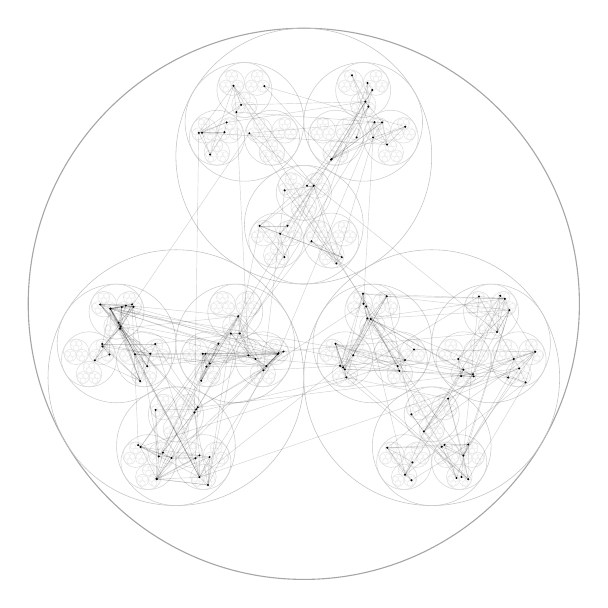
\begin{tikzpicture}[x=3.5cm, y=3.5cm]
% Generated by scripts/generate_padic_sirg.py: p=3, seed=42, vertices=129, line width=0.16pt, opacity=0.18
% Recursive p-adic ball hierarchy
\draw[thin, gray!70] (0,0) circle (1);
\draw[very thin, gray!48] (0,0.535898385) circle (0.464101615);
\draw[very thin, gray!48] (-0.464101615,-0.267949192) circle (0.464101615);
\draw[very thin, gray!48] (0.464101615,-0.267949192) circle (0.464101615);
\draw[very thin, gray!41] (-0.215390309,0.660254038) circle (0.215390309);
\draw[very thin, gray!41] (0,0.287187079) circle (0.215390309);
\draw[very thin, gray!41] (0.215390309,0.660254038) circle (0.215390309);
\draw[very thin, gray!41] (-0.679491924,-0.143593539) circle (0.215390309);
\draw[very thin, gray!41] (-0.464101615,-0.516660498) circle (0.215390309);
\draw[very thin, gray!41] (-0.248711306,-0.143593539) circle (0.215390309);
\draw[very thin, gray!41] (0.248711306,-0.143593539) circle (0.215390309);
\draw[very thin, gray!41] (0.464101615,-0.516660498) circle (0.215390309);
\draw[very thin, gray!41] (0.679491924,-0.143593539) circle (0.215390309);
\draw[very thin, gray!34] (-0.3153533,0.602540378) circle (0.09996299);
\draw[very thin, gray!34] (-0.115427319,0.602540378) circle (0.09996299);
\draw[very thin, gray!34] (-0.215390309,0.775681357) circle (0.09996299);
\draw[very thin, gray!34] (-0.09996299,0.229473419) circle (0.09996299);
\draw[very thin, gray!34] (0.09996299,0.229473419) circle (0.09996299);
\draw[very thin, gray!34] (0,0.402614398) circle (0.09996299);
\draw[very thin, gray!34] (0.115427319,0.602540378) circle (0.09996299);
\draw[very thin, gray!34] (0.3153533,0.602540378) circle (0.09996299);
\draw[very thin, gray!34] (0.215390309,0.775681357) circle (0.09996299);
\draw[very thin, gray!34] (-0.779454915,-0.201307199) circle (0.09996299);
\draw[very thin, gray!34] (-0.579528934,-0.201307199) circle (0.09996299);
\draw[very thin, gray!34] (-0.679491924,-0.028166221) circle (0.09996299);
\draw[very thin, gray!34] (-0.564064606,-0.574374158) circle (0.09996299);
\draw[very thin, gray!34] (-0.364138625,-0.574374158) circle (0.09996299);
\draw[very thin, gray!34] (-0.464101615,-0.40123318) circle (0.09996299);
\draw[very thin, gray!34] (-0.348674296,-0.201307199) circle (0.09996299);
\draw[very thin, gray!34] (-0.148748316,-0.201307199) circle (0.09996299);
\draw[very thin, gray!34] (-0.248711306,-0.028166221) circle (0.09996299);
\draw[very thin, gray!34] (0.148748316,-0.201307199) circle (0.09996299);
\draw[very thin, gray!34] (0.348674296,-0.201307199) circle (0.09996299);
\draw[very thin, gray!34] (0.248711306,-0.028166221) circle (0.09996299);
\draw[very thin, gray!34] (0.364138625,-0.574374158) circle (0.09996299);
\draw[very thin, gray!34] (0.564064606,-0.574374158) circle (0.09996299);
\draw[very thin, gray!34] (0.464101615,-0.40123318) circle (0.09996299);
\draw[very thin, gray!34] (0.579528934,-0.201307199) circle (0.09996299);
\draw[very thin, gray!34] (0.779454915,-0.201307199) circle (0.09996299);
\draw[very thin, gray!34] (0.679491924,-0.028166221) circle (0.09996299);
\draw[very thin, gray!27] (-0.3153533,0.548970373) circle (0.046392985);
\draw[very thin, gray!27] (-0.268960314,0.629325381) circle (0.046392985);
\draw[very thin, gray!27] (-0.361746285,0.629325381) circle (0.046392985);
\draw[very thin, gray!27] (-0.115427319,0.548970373) circle (0.046392985);
\draw[very thin, gray!27] (-0.069034334,0.629325381) circle (0.046392985);
\draw[very thin, gray!27] (-0.161820304,0.629325381) circle (0.046392985);
\draw[very thin, gray!27] (-0.215390309,0.722111352) circle (0.046392985);
\draw[very thin, gray!27] (-0.168997324,0.802466359) circle (0.046392985);
\draw[very thin, gray!27] (-0.261783294,0.802466359) circle (0.046392985);
\draw[very thin, gray!27] (-0.09996299,0.175903414) circle (0.046392985);
\draw[very thin, gray!27] (-0.053570005,0.256258422) circle (0.046392985);
\draw[very thin, gray!27] (-0.146355976,0.256258422) circle (0.046392985);
\draw[very thin, gray!27] (0.09996299,0.175903414) circle (0.046392985);
\draw[very thin, gray!27] (0.146355976,0.256258422) circle (0.046392985);
\draw[very thin, gray!27] (0.053570005,0.256258422) circle (0.046392985);
\draw[very thin, gray!27] (0,0.349044393) circle (0.046392985);
\draw[very thin, gray!27] (0.046392985,0.4293994) circle (0.046392985);
\draw[very thin, gray!27] (-0.046392985,0.4293994) circle (0.046392985);
\draw[very thin, gray!27] (0.115427319,0.548970373) circle (0.046392985);
\draw[very thin, gray!27] (0.161820304,0.629325381) circle (0.046392985);
\draw[very thin, gray!27] (0.069034334,0.629325381) circle (0.046392985);
\draw[very thin, gray!27] (0.3153533,0.548970373) circle (0.046392985);
\draw[very thin, gray!27] (0.361746285,0.629325381) circle (0.046392985);
\draw[very thin, gray!27] (0.268960314,0.629325381) circle (0.046392985);
\draw[very thin, gray!27] (0.215390309,0.722111352) circle (0.046392985);
\draw[very thin, gray!27] (0.261783294,0.802466359) circle (0.046392985);
\draw[very thin, gray!27] (0.168997324,0.802466359) circle (0.046392985);
\draw[very thin, gray!27] (-0.779454915,-0.254877204) circle (0.046392985);
\draw[very thin, gray!27] (-0.733061929,-0.174522196) circle (0.046392985);
\draw[very thin, gray!27] (-0.8258479,-0.174522196) circle (0.046392985);
\draw[very thin, gray!27] (-0.579528934,-0.254877204) circle (0.046392985);
\draw[very thin, gray!27] (-0.533135949,-0.174522196) circle (0.046392985);
\draw[very thin, gray!27] (-0.625921919,-0.174522196) circle (0.046392985);
\draw[very thin, gray!27] (-0.679491924,-0.081736226) circle (0.046392985);
\draw[very thin, gray!27] (-0.633098939,-0.001381218) circle (0.046392985);
\draw[very thin, gray!27] (-0.72588491,-0.001381218) circle (0.046392985);
\draw[very thin, gray!27] (-0.564064606,-0.627944163) circle (0.046392985);
\draw[very thin, gray!27] (-0.51767162,-0.547589155) circle (0.046392985);
\draw[very thin, gray!27] (-0.610457591,-0.547589155) circle (0.046392985);
\draw[very thin, gray!27] (-0.364138625,-0.627944163) circle (0.046392985);
\draw[very thin, gray!27] (-0.317745639,-0.547589155) circle (0.046392985);
\draw[very thin, gray!27] (-0.41053161,-0.547589155) circle (0.046392985);
\draw[very thin, gray!27] (-0.464101615,-0.454803185) circle (0.046392985);
\draw[very thin, gray!27] (-0.41770863,-0.374448177) circle (0.046392985);
\draw[very thin, gray!27] (-0.5104946,-0.374448177) circle (0.046392985);
\draw[very thin, gray!27] (-0.348674296,-0.254877204) circle (0.046392985);
\draw[very thin, gray!27] (-0.302281311,-0.174522196) circle (0.046392985);
\draw[very thin, gray!27] (-0.395067282,-0.174522196) circle (0.046392985);
\draw[very thin, gray!27] (-0.148748316,-0.254877204) circle (0.046392985);
\draw[very thin, gray!27] (-0.10235533,-0.174522196) circle (0.046392985);
\draw[very thin, gray!27] (-0.195141301,-0.174522196) circle (0.046392985);
\draw[very thin, gray!27] (-0.248711306,-0.081736226) circle (0.046392985);
\draw[very thin, gray!27] (-0.202318321,-0.001381218) circle (0.046392985);
\draw[very thin, gray!27] (-0.295104291,-0.001381218) circle (0.046392985);
\draw[very thin, gray!27] (0.148748316,-0.254877204) circle (0.046392985);
\draw[very thin, gray!27] (0.195141301,-0.174522196) circle (0.046392985);
\draw[very thin, gray!27] (0.10235533,-0.174522196) circle (0.046392985);
\draw[very thin, gray!27] (0.348674296,-0.254877204) circle (0.046392985);
\draw[very thin, gray!27] (0.395067282,-0.174522196) circle (0.046392985);
\draw[very thin, gray!27] (0.302281311,-0.174522196) circle (0.046392985);
\draw[very thin, gray!27] (0.248711306,-0.081736226) circle (0.046392985);
\draw[very thin, gray!27] (0.295104291,-0.001381218) circle (0.046392985);
\draw[very thin, gray!27] (0.202318321,-0.001381218) circle (0.046392985);
\draw[very thin, gray!27] (0.364138625,-0.627944163) circle (0.046392985);
\draw[very thin, gray!27] (0.41053161,-0.547589155) circle (0.046392985);
\draw[very thin, gray!27] (0.317745639,-0.547589155) circle (0.046392985);
\draw[very thin, gray!27] (0.564064606,-0.627944163) circle (0.046392985);
\draw[very thin, gray!27] (0.610457591,-0.547589155) circle (0.046392985);
\draw[very thin, gray!27] (0.51767162,-0.547589155) circle (0.046392985);
\draw[very thin, gray!27] (0.464101615,-0.454803185) circle (0.046392985);
\draw[very thin, gray!27] (0.5104946,-0.374448177) circle (0.046392985);
\draw[very thin, gray!27] (0.41770863,-0.374448177) circle (0.046392985);
\draw[very thin, gray!27] (0.579528934,-0.254877204) circle (0.046392985);
\draw[very thin, gray!27] (0.625921919,-0.174522196) circle (0.046392985);
\draw[very thin, gray!27] (0.533135949,-0.174522196) circle (0.046392985);
\draw[very thin, gray!27] (0.779454915,-0.254877204) circle (0.046392985);
\draw[very thin, gray!27] (0.8258479,-0.174522196) circle (0.046392985);
\draw[very thin, gray!27] (0.733061929,-0.174522196) circle (0.046392985);
\draw[very thin, gray!27] (0.679491924,-0.081736226) circle (0.046392985);
\draw[very thin, gray!27] (0.72588491,-0.001381218) circle (0.046392985);
\draw[very thin, gray!27] (0.633098939,-0.001381218) circle (0.046392985);
\draw[very thin, gray!20] (-0.29382224,0.53653941) circle (0.021531059);
\draw[very thin, gray!20] (-0.3153533,0.573832299) circle (0.021531059);
\draw[very thin, gray!20] (-0.336884359,0.53653941) circle (0.021531059);
\draw[very thin, gray!20] (-0.247429255,0.616894418) circle (0.021531059);
\draw[very thin, gray!20] (-0.268960314,0.654187307) circle (0.021531059);
\draw[very thin, gray!20] (-0.290491374,0.616894418) circle (0.021531059);
\draw[very thin, gray!20] (-0.340215225,0.616894418) circle (0.021531059);
\draw[very thin, gray!20] (-0.361746285,0.654187307) circle (0.021531059);
\draw[very thin, gray!20] (-0.383277344,0.616894418) circle (0.021531059);
\draw[very thin, gray!20] (-0.093896259,0.53653941) circle (0.021531059);
\draw[very thin, gray!20] (-0.115427319,0.573832299) circle (0.021531059);
\draw[very thin, gray!20] (-0.136958378,0.53653941) circle (0.021531059);
\draw[very thin, gray!20] (-0.047503274,0.616894418) circle (0.021531059);
\draw[very thin, gray!20] (-0.069034334,0.654187307) circle (0.021531059);
\draw[very thin, gray!20] (-0.090565393,0.616894418) circle (0.021531059);
\draw[very thin, gray!20] (-0.140289245,0.616894418) circle (0.021531059);
\draw[very thin, gray!20] (-0.161820304,0.654187307) circle (0.021531059);
\draw[very thin, gray!20] (-0.183351363,0.616894418) circle (0.021531059);
\draw[very thin, gray!20] (-0.19385925,0.709680389) circle (0.021531059);
\draw[very thin, gray!20] (-0.215390309,0.746973277) circle (0.021531059);
\draw[very thin, gray!20] (-0.236921369,0.709680389) circle (0.021531059);
\draw[very thin, gray!20] (-0.147466264,0.790035396) circle (0.021531059);
\draw[very thin, gray!20] (-0.168997324,0.827328285) circle (0.021531059);
\draw[very thin, gray!20] (-0.190528383,0.790035396) circle (0.021531059);
\draw[very thin, gray!20] (-0.240252235,0.790035396) circle (0.021531059);
\draw[very thin, gray!20] (-0.261783294,0.827328285) circle (0.021531059);
\draw[very thin, gray!20] (-0.283314354,0.790035396) circle (0.021531059);
\draw[very thin, gray!20] (-0.078431931,0.163472451) circle (0.021531059);
\draw[very thin, gray!20] (-0.09996299,0.20076534) circle (0.021531059);
\draw[very thin, gray!20] (-0.12149405,0.163472451) circle (0.021531059);
\draw[very thin, gray!20] (-0.032038946,0.243827459) circle (0.021531059);
\draw[very thin, gray!20] (-0.053570005,0.281120348) circle (0.021531059);
\draw[very thin, gray!20] (-0.075101064,0.243827459) circle (0.021531059);
\draw[very thin, gray!20] (-0.124824916,0.243827459) circle (0.021531059);
\draw[very thin, gray!20] (-0.146355976,0.281120348) circle (0.021531059);
\draw[very thin, gray!20] (-0.167887035,0.243827459) circle (0.021531059);
\draw[very thin, gray!20] (0.12149405,0.163472451) circle (0.021531059);
\draw[very thin, gray!20] (0.09996299,0.20076534) circle (0.021531059);
\draw[very thin, gray!20] (0.078431931,0.163472451) circle (0.021531059);
\draw[very thin, gray!20] (0.167887035,0.243827459) circle (0.021531059);
\draw[very thin, gray!20] (0.146355976,0.281120348) circle (0.021531059);
\draw[very thin, gray!20] (0.124824916,0.243827459) circle (0.021531059);
\draw[very thin, gray!20] (0.075101064,0.243827459) circle (0.021531059);
\draw[very thin, gray!20] (0.053570005,0.281120348) circle (0.021531059);
\draw[very thin, gray!20] (0.032038946,0.243827459) circle (0.021531059);
\draw[very thin, gray!20] (0.021531059,0.33661343) circle (0.021531059);
\draw[very thin, gray!20] (0,0.373906318) circle (0.021531059);
\draw[very thin, gray!20] (-0.021531059,0.33661343) circle (0.021531059);
\draw[very thin, gray!20] (0.067924045,0.416968437) circle (0.021531059);
\draw[very thin, gray!20] (0.046392985,0.454261326) circle (0.021531059);
\draw[very thin, gray!20] (0.024861926,0.416968437) circle (0.021531059);
\draw[very thin, gray!20] (-0.024861926,0.416968437) circle (0.021531059);
\draw[very thin, gray!20] (-0.046392985,0.454261326) circle (0.021531059);
\draw[very thin, gray!20] (-0.067924045,0.416968437) circle (0.021531059);
\draw[very thin, gray!20] (0.136958378,0.53653941) circle (0.021531059);
\draw[very thin, gray!20] (0.115427319,0.573832299) circle (0.021531059);
\draw[very thin, gray!20] (0.093896259,0.53653941) circle (0.021531059);
\draw[very thin, gray!20] (0.183351363,0.616894418) circle (0.021531059);
\draw[very thin, gray!20] (0.161820304,0.654187307) circle (0.021531059);
\draw[very thin, gray!20] (0.140289245,0.616894418) circle (0.021531059);
\draw[very thin, gray!20] (0.090565393,0.616894418) circle (0.021531059);
\draw[very thin, gray!20] (0.069034334,0.654187307) circle (0.021531059);
\draw[very thin, gray!20] (0.047503274,0.616894418) circle (0.021531059);
\draw[very thin, gray!20] (0.336884359,0.53653941) circle (0.021531059);
\draw[very thin, gray!20] (0.3153533,0.573832299) circle (0.021531059);
\draw[very thin, gray!20] (0.29382224,0.53653941) circle (0.021531059);
\draw[very thin, gray!20] (0.383277344,0.616894418) circle (0.021531059);
\draw[very thin, gray!20] (0.361746285,0.654187307) circle (0.021531059);
\draw[very thin, gray!20] (0.340215225,0.616894418) circle (0.021531059);
\draw[very thin, gray!20] (0.290491374,0.616894418) circle (0.021531059);
\draw[very thin, gray!20] (0.268960314,0.654187307) circle (0.021531059);
\draw[very thin, gray!20] (0.247429255,0.616894418) circle (0.021531059);
\draw[very thin, gray!20] (0.236921369,0.709680389) circle (0.021531059);
\draw[very thin, gray!20] (0.215390309,0.746973277) circle (0.021531059);
\draw[very thin, gray!20] (0.19385925,0.709680389) circle (0.021531059);
\draw[very thin, gray!20] (0.283314354,0.790035396) circle (0.021531059);
\draw[very thin, gray!20] (0.261783294,0.827328285) circle (0.021531059);
\draw[very thin, gray!20] (0.240252235,0.790035396) circle (0.021531059);
\draw[very thin, gray!20] (0.190528383,0.790035396) circle (0.021531059);
\draw[very thin, gray!20] (0.168997324,0.827328285) circle (0.021531059);
\draw[very thin, gray!20] (0.147466264,0.790035396) circle (0.021531059);
\draw[very thin, gray!20] (-0.757923855,-0.267308167) circle (0.021531059);
\draw[very thin, gray!20] (-0.779454915,-0.230015278) circle (0.021531059);
\draw[very thin, gray!20] (-0.800985974,-0.267308167) circle (0.021531059);
\draw[very thin, gray!20] (-0.71153087,-0.186953159) circle (0.021531059);
\draw[very thin, gray!20] (-0.733061929,-0.14966027) circle (0.021531059);
\draw[very thin, gray!20] (-0.754592989,-0.186953159) circle (0.021531059);
\draw[very thin, gray!20] (-0.804316841,-0.186953159) circle (0.021531059);
\draw[very thin, gray!20] (-0.8258479,-0.14966027) circle (0.021531059);
\draw[very thin, gray!20] (-0.847378959,-0.186953159) circle (0.021531059);
\draw[very thin, gray!20] (-0.557997875,-0.267308167) circle (0.021531059);
\draw[very thin, gray!20] (-0.579528934,-0.230015278) circle (0.021531059);
\draw[very thin, gray!20] (-0.601059993,-0.267308167) circle (0.021531059);
\draw[very thin, gray!20] (-0.511604889,-0.186953159) circle (0.021531059);
\draw[very thin, gray!20] (-0.533135949,-0.14966027) circle (0.021531059);
\draw[very thin, gray!20] (-0.554667008,-0.186953159) circle (0.021531059);
\draw[very thin, gray!20] (-0.60439086,-0.186953159) circle (0.021531059);
\draw[very thin, gray!20] (-0.625921919,-0.14966027) circle (0.021531059);
\draw[very thin, gray!20] (-0.647452979,-0.186953159) circle (0.021531059);
\draw[very thin, gray!20] (-0.657960865,-0.094167189) circle (0.021531059);
\draw[very thin, gray!20] (-0.679491924,-0.0568743) circle (0.021531059);
\draw[very thin, gray!20] (-0.701022984,-0.094167189) circle (0.021531059);
\draw[very thin, gray!20] (-0.61156788,-0.013812181) circle (0.021531059);
\draw[very thin, gray!20] (-0.633098939,0.023480708) circle (0.021531059);
\draw[very thin, gray!20] (-0.654629998,-0.013812181) circle (0.021531059);
\draw[very thin, gray!20] (-0.70435385,-0.013812181) circle (0.021531059);
\draw[very thin, gray!20] (-0.72588491,0.023480708) circle (0.021531059);
\draw[very thin, gray!20] (-0.747415969,-0.013812181) circle (0.021531059);
\draw[very thin, gray!20] (-0.542533546,-0.640375126) circle (0.021531059);
\draw[very thin, gray!20] (-0.564064606,-0.603082237) circle (0.021531059);
\draw[very thin, gray!20] (-0.585595665,-0.640375126) circle (0.021531059);
\draw[very thin, gray!20] (-0.496140561,-0.560020118) circle (0.021531059);
\draw[very thin, gray!20] (-0.51767162,-0.522727229) circle (0.021531059);
\draw[very thin, gray!20] (-0.53920268,-0.560020118) circle (0.021531059);
\draw[very thin, gray!20] (-0.588926531,-0.560020118) circle (0.021531059);
\draw[very thin, gray!20] (-0.610457591,-0.522727229) circle (0.021531059);
\draw[very thin, gray!20] (-0.63198865,-0.560020118) circle (0.021531059);
\draw[very thin, gray!20] (-0.342607565,-0.640375126) circle (0.021531059);
\draw[very thin, gray!20] (-0.364138625,-0.603082237) circle (0.021531059);
\draw[very thin, gray!20] (-0.385669684,-0.640375126) circle (0.021531059);
\draw[very thin, gray!20] (-0.29621458,-0.560020118) circle (0.021531059);
\draw[very thin, gray!20] (-0.317745639,-0.522727229) circle (0.021531059);
\draw[very thin, gray!20] (-0.339276699,-0.560020118) circle (0.021531059);
\draw[very thin, gray!20] (-0.389000551,-0.560020118) circle (0.021531059);
\draw[very thin, gray!20] (-0.41053161,-0.522727229) circle (0.021531059);
\draw[very thin, gray!20] (-0.432062669,-0.560020118) circle (0.021531059);
\draw[very thin, gray!20] (-0.442570556,-0.467234148) circle (0.021531059);
\draw[very thin, gray!20] (-0.464101615,-0.429941259) circle (0.021531059);
\draw[very thin, gray!20] (-0.485632675,-0.467234148) circle (0.021531059);
\draw[very thin, gray!20] (-0.39617757,-0.38687914) circle (0.021531059);
\draw[very thin, gray!20] (-0.41770863,-0.349586251) circle (0.021531059);
\draw[very thin, gray!20] (-0.439239689,-0.38687914) circle (0.021531059);
\draw[very thin, gray!20] (-0.488963541,-0.38687914) circle (0.021531059);
\draw[very thin, gray!20] (-0.5104946,-0.349586251) circle (0.021531059);
\draw[very thin, gray!20] (-0.53202566,-0.38687914) circle (0.021531059);
\draw[very thin, gray!20] (-0.327143237,-0.267308167) circle (0.021531059);
\draw[very thin, gray!20] (-0.348674296,-0.230015278) circle (0.021531059);
\draw[very thin, gray!20] (-0.370205356,-0.267308167) circle (0.021531059);
\draw[very thin, gray!20] (-0.280750252,-0.186953159) circle (0.021531059);
\draw[very thin, gray!20] (-0.302281311,-0.14966027) circle (0.021531059);
\draw[very thin, gray!20] (-0.32381237,-0.186953159) circle (0.021531059);
\draw[very thin, gray!20] (-0.373536222,-0.186953159) circle (0.021531059);
\draw[very thin, gray!20] (-0.395067282,-0.14966027) circle (0.021531059);
\draw[very thin, gray!20] (-0.416598341,-0.186953159) circle (0.021531059);
\draw[very thin, gray!20] (-0.127217256,-0.267308167) circle (0.021531059);
\draw[very thin, gray!20] (-0.148748316,-0.230015278) circle (0.021531059);
\draw[very thin, gray!20] (-0.170279375,-0.267308167) circle (0.021531059);
\draw[very thin, gray!20] (-0.080824271,-0.186953159) circle (0.021531059);
\draw[very thin, gray!20] (-0.10235533,-0.14966027) circle (0.021531059);
\draw[very thin, gray!20] (-0.12388639,-0.186953159) circle (0.021531059);
\draw[very thin, gray!20] (-0.173610241,-0.186953159) circle (0.021531059);
\draw[very thin, gray!20] (-0.195141301,-0.14966027) circle (0.021531059);
\draw[very thin, gray!20] (-0.21667236,-0.186953159) circle (0.021531059);
\draw[very thin, gray!20] (-0.227180247,-0.094167189) circle (0.021531059);
\draw[very thin, gray!20] (-0.248711306,-0.0568743) circle (0.021531059);
\draw[very thin, gray!20] (-0.270242365,-0.094167189) circle (0.021531059);
\draw[very thin, gray!20] (-0.180787261,-0.013812181) circle (0.021531059);
\draw[very thin, gray!20] (-0.202318321,0.023480708) circle (0.021531059);
\draw[very thin, gray!20] (-0.22384938,-0.013812181) circle (0.021531059);
\draw[very thin, gray!20] (-0.273573232,-0.013812181) circle (0.021531059);
\draw[very thin, gray!20] (-0.295104291,0.023480708) circle (0.021531059);
\draw[very thin, gray!20] (-0.316635351,-0.013812181) circle (0.021531059);
\draw[very thin, gray!20] (0.170279375,-0.267308167) circle (0.021531059);
\draw[very thin, gray!20] (0.148748316,-0.230015278) circle (0.021531059);
\draw[very thin, gray!20] (0.127217256,-0.267308167) circle (0.021531059);
\draw[very thin, gray!20] (0.21667236,-0.186953159) circle (0.021531059);
\draw[very thin, gray!20] (0.195141301,-0.14966027) circle (0.021531059);
\draw[very thin, gray!20] (0.173610241,-0.186953159) circle (0.021531059);
\draw[very thin, gray!20] (0.12388639,-0.186953159) circle (0.021531059);
\draw[very thin, gray!20] (0.10235533,-0.14966027) circle (0.021531059);
\draw[very thin, gray!20] (0.080824271,-0.186953159) circle (0.021531059);
\draw[very thin, gray!20] (0.370205356,-0.267308167) circle (0.021531059);
\draw[very thin, gray!20] (0.348674296,-0.230015278) circle (0.021531059);
\draw[very thin, gray!20] (0.327143237,-0.267308167) circle (0.021531059);
\draw[very thin, gray!20] (0.416598341,-0.186953159) circle (0.021531059);
\draw[very thin, gray!20] (0.395067282,-0.14966027) circle (0.021531059);
\draw[very thin, gray!20] (0.373536222,-0.186953159) circle (0.021531059);
\draw[very thin, gray!20] (0.32381237,-0.186953159) circle (0.021531059);
\draw[very thin, gray!20] (0.302281311,-0.14966027) circle (0.021531059);
\draw[very thin, gray!20] (0.280750252,-0.186953159) circle (0.021531059);
\draw[very thin, gray!20] (0.270242365,-0.094167189) circle (0.021531059);
\draw[very thin, gray!20] (0.248711306,-0.0568743) circle (0.021531059);
\draw[very thin, gray!20] (0.227180247,-0.094167189) circle (0.021531059);
\draw[very thin, gray!20] (0.316635351,-0.013812181) circle (0.021531059);
\draw[very thin, gray!20] (0.295104291,0.023480708) circle (0.021531059);
\draw[very thin, gray!20] (0.273573232,-0.013812181) circle (0.021531059);
\draw[very thin, gray!20] (0.22384938,-0.013812181) circle (0.021531059);
\draw[very thin, gray!20] (0.202318321,0.023480708) circle (0.021531059);
\draw[very thin, gray!20] (0.180787261,-0.013812181) circle (0.021531059);
\draw[very thin, gray!20] (0.385669684,-0.640375126) circle (0.021531059);
\draw[very thin, gray!20] (0.364138625,-0.603082237) circle (0.021531059);
\draw[very thin, gray!20] (0.342607565,-0.640375126) circle (0.021531059);
\draw[very thin, gray!20] (0.432062669,-0.560020118) circle (0.021531059);
\draw[very thin, gray!20] (0.41053161,-0.522727229) circle (0.021531059);
\draw[very thin, gray!20] (0.389000551,-0.560020118) circle (0.021531059);
\draw[very thin, gray!20] (0.339276699,-0.560020118) circle (0.021531059);
\draw[very thin, gray!20] (0.317745639,-0.522727229) circle (0.021531059);
\draw[very thin, gray!20] (0.29621458,-0.560020118) circle (0.021531059);
\draw[very thin, gray!20] (0.585595665,-0.640375126) circle (0.021531059);
\draw[very thin, gray!20] (0.564064606,-0.603082237) circle (0.021531059);
\draw[very thin, gray!20] (0.542533546,-0.640375126) circle (0.021531059);
\draw[very thin, gray!20] (0.63198865,-0.560020118) circle (0.021531059);
\draw[very thin, gray!20] (0.610457591,-0.522727229) circle (0.021531059);
\draw[very thin, gray!20] (0.588926531,-0.560020118) circle (0.021531059);
\draw[very thin, gray!20] (0.53920268,-0.560020118) circle (0.021531059);
\draw[very thin, gray!20] (0.51767162,-0.522727229) circle (0.021531059);
\draw[very thin, gray!20] (0.496140561,-0.560020118) circle (0.021531059);
\draw[very thin, gray!20] (0.485632675,-0.467234148) circle (0.021531059);
\draw[very thin, gray!20] (0.464101615,-0.429941259) circle (0.021531059);
\draw[very thin, gray!20] (0.442570556,-0.467234148) circle (0.021531059);
\draw[very thin, gray!20] (0.53202566,-0.38687914) circle (0.021531059);
\draw[very thin, gray!20] (0.5104946,-0.349586251) circle (0.021531059);
\draw[very thin, gray!20] (0.488963541,-0.38687914) circle (0.021531059);
\draw[very thin, gray!20] (0.439239689,-0.38687914) circle (0.021531059);
\draw[very thin, gray!20] (0.41770863,-0.349586251) circle (0.021531059);
\draw[very thin, gray!20] (0.39617757,-0.38687914) circle (0.021531059);
\draw[very thin, gray!20] (0.601059993,-0.267308167) circle (0.021531059);
\draw[very thin, gray!20] (0.579528934,-0.230015278) circle (0.021531059);
\draw[very thin, gray!20] (0.557997875,-0.267308167) circle (0.021531059);
\draw[very thin, gray!20] (0.647452979,-0.186953159) circle (0.021531059);
\draw[very thin, gray!20] (0.625921919,-0.14966027) circle (0.021531059);
\draw[very thin, gray!20] (0.60439086,-0.186953159) circle (0.021531059);
\draw[very thin, gray!20] (0.554667008,-0.186953159) circle (0.021531059);
\draw[very thin, gray!20] (0.533135949,-0.14966027) circle (0.021531059);
\draw[very thin, gray!20] (0.511604889,-0.186953159) circle (0.021531059);
\draw[very thin, gray!20] (0.800985974,-0.267308167) circle (0.021531059);
\draw[very thin, gray!20] (0.779454915,-0.230015278) circle (0.021531059);
\draw[very thin, gray!20] (0.757923855,-0.267308167) circle (0.021531059);
\draw[very thin, gray!20] (0.847378959,-0.186953159) circle (0.021531059);
\draw[very thin, gray!20] (0.8258479,-0.14966027) circle (0.021531059);
\draw[very thin, gray!20] (0.804316841,-0.186953159) circle (0.021531059);
\draw[very thin, gray!20] (0.754592989,-0.186953159) circle (0.021531059);
\draw[very thin, gray!20] (0.733061929,-0.14966027) circle (0.021531059);
\draw[very thin, gray!20] (0.71153087,-0.186953159) circle (0.021531059);
\draw[very thin, gray!20] (0.701022984,-0.094167189) circle (0.021531059);
\draw[very thin, gray!20] (0.679491924,-0.0568743) circle (0.021531059);
\draw[very thin, gray!20] (0.657960865,-0.094167189) circle (0.021531059);
\draw[very thin, gray!20] (0.747415969,-0.013812181) circle (0.021531059);
\draw[very thin, gray!20] (0.72588491,0.023480708) circle (0.021531059);
\draw[very thin, gray!20] (0.70435385,-0.013812181) circle (0.021531059);
\draw[very thin, gray!20] (0.654629998,-0.013812181) circle (0.021531059);
\draw[very thin, gray!20] (0.633098939,0.023480708) circle (0.021531059);
\draw[very thin, gray!20] (0.61156788,-0.013812181) circle (0.021531059);
\draw[very thin, gray!15] (-0.283829641,0.54230864) circle (0.009992599);
\draw[very thin, gray!15] (-0.30381484,0.54230864) circle (0.009992599);
\draw[very thin, gray!15] (-0.29382224,0.52500095) circle (0.009992599);
\draw[very thin, gray!15] (-0.3053607,0.579601529) circle (0.009992599);
\draw[very thin, gray!15] (-0.325345899,0.579601529) circle (0.009992599);
\draw[very thin, gray!15] (-0.3153533,0.562293839) circle (0.009992599);
\draw[very thin, gray!15] (-0.32689176,0.54230864) circle (0.009992599);
\draw[very thin, gray!15] (-0.346876958,0.54230864) circle (0.009992599);
\draw[very thin, gray!15] (-0.336884359,0.52500095) circle (0.009992599);
\draw[very thin, gray!15] (-0.237436655,0.622663648) circle (0.009992599);
\draw[very thin, gray!15] (-0.257421854,0.622663648) circle (0.009992599);
\draw[very thin, gray!15] (-0.247429255,0.605355958) circle (0.009992599);
\draw[very thin, gray!15] (-0.258967715,0.659956537) circle (0.009992599);
\draw[very thin, gray!15] (-0.278952914,0.659956537) circle (0.009992599);
\draw[very thin, gray!15] (-0.268960314,0.642648847) circle (0.009992599);
\draw[very thin, gray!15] (-0.280498774,0.622663648) circle (0.009992599);
\draw[very thin, gray!15] (-0.300483973,0.622663648) circle (0.009992599);
\draw[very thin, gray!15] (-0.290491374,0.605355958) circle (0.009992599);
\draw[very thin, gray!15] (-0.330222626,0.622663648) circle (0.009992599);
\draw[very thin, gray!15] (-0.350207825,0.622663648) circle (0.009992599);
\draw[very thin, gray!15] (-0.340215225,0.605355958) circle (0.009992599);
\draw[very thin, gray!15] (-0.351753685,0.659956537) circle (0.009992599);
\draw[very thin, gray!15] (-0.371738884,0.659956537) circle (0.009992599);
\draw[very thin, gray!15] (-0.361746285,0.642648847) circle (0.009992599);
\draw[very thin, gray!15] (-0.373284745,0.622663648) circle (0.009992599);
\draw[very thin, gray!15] (-0.393269944,0.622663648) circle (0.009992599);
\draw[very thin, gray!15] (-0.383277344,0.605355958) circle (0.009992599);
\draw[very thin, gray!15] (-0.08390366,0.54230864) circle (0.009992599);
\draw[very thin, gray!15] (-0.103888859,0.54230864) circle (0.009992599);
\draw[very thin, gray!15] (-0.093896259,0.52500095) circle (0.009992599);
\draw[very thin, gray!15] (-0.105434719,0.579601529) circle (0.009992599);
\draw[very thin, gray!15] (-0.125419918,0.579601529) circle (0.009992599);
\draw[very thin, gray!15] (-0.115427319,0.562293839) circle (0.009992599);
\draw[very thin, gray!15] (-0.126965779,0.54230864) circle (0.009992599);
\draw[very thin, gray!15] (-0.146950978,0.54230864) circle (0.009992599);
\draw[very thin, gray!15] (-0.136958378,0.52500095) circle (0.009992599);
\draw[very thin, gray!15] (-0.037510675,0.622663648) circle (0.009992599);
\draw[very thin, gray!15] (-0.057495874,0.622663648) circle (0.009992599);
\draw[very thin, gray!15] (-0.047503274,0.605355958) circle (0.009992599);
\draw[very thin, gray!15] (-0.059041734,0.659956537) circle (0.009992599);
\draw[very thin, gray!15] (-0.079026933,0.659956537) circle (0.009992599);
\draw[very thin, gray!15] (-0.069034334,0.642648847) circle (0.009992599);
\draw[very thin, gray!15] (-0.080572793,0.622663648) circle (0.009992599);
\draw[very thin, gray!15] (-0.100557992,0.622663648) circle (0.009992599);
\draw[very thin, gray!15] (-0.090565393,0.605355958) circle (0.009992599);
\draw[very thin, gray!15] (-0.130296645,0.622663648) circle (0.009992599);
\draw[very thin, gray!15] (-0.150281844,0.622663648) circle (0.009992599);
\draw[very thin, gray!15] (-0.140289245,0.605355958) circle (0.009992599);
\draw[very thin, gray!15] (-0.151827705,0.659956537) circle (0.009992599);
\draw[very thin, gray!15] (-0.171812904,0.659956537) circle (0.009992599);
\draw[very thin, gray!15] (-0.161820304,0.642648847) circle (0.009992599);
\draw[very thin, gray!15] (-0.173358764,0.622663648) circle (0.009992599);
\draw[very thin, gray!15] (-0.193343963,0.622663648) circle (0.009992599);
\draw[very thin, gray!15] (-0.183351363,0.605355958) circle (0.009992599);
\draw[very thin, gray!15] (-0.18386665,0.715449619) circle (0.009992599);
\draw[very thin, gray!15] (-0.203851849,0.715449619) circle (0.009992599);
\draw[very thin, gray!15] (-0.19385925,0.698141929) circle (0.009992599);
\draw[very thin, gray!15] (-0.20539771,0.752742507) circle (0.009992599);
\draw[very thin, gray!15] (-0.225382909,0.752742507) circle (0.009992599);
\draw[very thin, gray!15] (-0.215390309,0.735434817) circle (0.009992599);
\draw[very thin, gray!15] (-0.226928769,0.715449619) circle (0.009992599);
\draw[very thin, gray!15] (-0.246913968,0.715449619) circle (0.009992599);
\draw[very thin, gray!15] (-0.236921369,0.698141929) circle (0.009992599);
\draw[very thin, gray!15] (-0.137473665,0.795804626) circle (0.009992599);
\draw[very thin, gray!15] (-0.157458864,0.795804626) circle (0.009992599);
\draw[very thin, gray!15] (-0.147466264,0.778496936) circle (0.009992599);
\draw[very thin, gray!15] (-0.159004724,0.833097515) circle (0.009992599);
\draw[very thin, gray!15] (-0.178989923,0.833097515) circle (0.009992599);
\draw[very thin, gray!15] (-0.168997324,0.815789825) circle (0.009992599);
\draw[very thin, gray!15] (-0.180535784,0.795804626) circle (0.009992599);
\draw[very thin, gray!15] (-0.200520983,0.795804626) circle (0.009992599);
\draw[very thin, gray!15] (-0.190528383,0.778496936) circle (0.009992599);
\draw[very thin, gray!15] (-0.230259636,0.795804626) circle (0.009992599);
\draw[very thin, gray!15] (-0.250244835,0.795804626) circle (0.009992599);
\draw[very thin, gray!15] (-0.240252235,0.778496936) circle (0.009992599);
\draw[very thin, gray!15] (-0.251790695,0.833097515) circle (0.009992599);
\draw[very thin, gray!15] (-0.271775894,0.833097515) circle (0.009992599);
\draw[very thin, gray!15] (-0.261783294,0.815789825) circle (0.009992599);
\draw[very thin, gray!15] (-0.273321754,0.795804626) circle (0.009992599);
\draw[very thin, gray!15] (-0.293306953,0.795804626) circle (0.009992599);
\draw[very thin, gray!15] (-0.283314354,0.778496936) circle (0.009992599);
\draw[very thin, gray!15] (-0.068439332,0.169241681) circle (0.009992599);
\draw[very thin, gray!15] (-0.08842453,0.169241681) circle (0.009992599);
\draw[very thin, gray!15] (-0.078431931,0.151933992) circle (0.009992599);
\draw[very thin, gray!15] (-0.089970391,0.20653457) circle (0.009992599);
\draw[very thin, gray!15] (-0.10995559,0.20653457) circle (0.009992599);
\draw[very thin, gray!15] (-0.09996299,0.18922688) circle (0.009992599);
\draw[very thin, gray!15] (-0.11150145,0.169241681) circle (0.009992599);
\draw[very thin, gray!15] (-0.131486649,0.169241681) circle (0.009992599);
\draw[very thin, gray!15] (-0.12149405,0.151933992) circle (0.009992599);
\draw[very thin, gray!15] (-0.022046346,0.249596689) circle (0.009992599);
\draw[very thin, gray!15] (-0.042031545,0.249596689) circle (0.009992599);
\draw[very thin, gray!15] (-0.032038946,0.232288999) circle (0.009992599);
\draw[very thin, gray!15] (-0.043577406,0.286889578) circle (0.009992599);
\draw[very thin, gray!15] (-0.063562605,0.286889578) circle (0.009992599);
\draw[very thin, gray!15] (-0.053570005,0.269581888) circle (0.009992599);
\draw[very thin, gray!15] (-0.065108465,0.249596689) circle (0.009992599);
\draw[very thin, gray!15] (-0.085093664,0.249596689) circle (0.009992599);
\draw[very thin, gray!15] (-0.075101064,0.232288999) circle (0.009992599);
\draw[very thin, gray!15] (-0.114832317,0.249596689) circle (0.009992599);
\draw[very thin, gray!15] (-0.134817516,0.249596689) circle (0.009992599);
\draw[very thin, gray!15] (-0.124824916,0.232288999) circle (0.009992599);
\draw[very thin, gray!15] (-0.136363376,0.286889578) circle (0.009992599);
\draw[very thin, gray!15] (-0.156348575,0.286889578) circle (0.009992599);
\draw[very thin, gray!15] (-0.146355976,0.269581888) circle (0.009992599);
\draw[very thin, gray!15] (-0.157894436,0.249596689) circle (0.009992599);
\draw[very thin, gray!15] (-0.177879635,0.249596689) circle (0.009992599);
\draw[very thin, gray!15] (-0.167887035,0.232288999) circle (0.009992599);
\draw[very thin, gray!15] (0.131486649,0.169241681) circle (0.009992599);
\draw[very thin, gray!15] (0.11150145,0.169241681) circle (0.009992599);
\draw[very thin, gray!15] (0.12149405,0.151933992) circle (0.009992599);
\draw[very thin, gray!15] (0.10995559,0.20653457) circle (0.009992599);
\draw[very thin, gray!15] (0.089970391,0.20653457) circle (0.009992599);
\draw[very thin, gray!15] (0.09996299,0.18922688) circle (0.009992599);
\draw[very thin, gray!15] (0.08842453,0.169241681) circle (0.009992599);
\draw[very thin, gray!15] (0.068439332,0.169241681) circle (0.009992599);
\draw[very thin, gray!15] (0.078431931,0.151933992) circle (0.009992599);
\draw[very thin, gray!15] (0.177879635,0.249596689) circle (0.009992599);
\draw[very thin, gray!15] (0.157894436,0.249596689) circle (0.009992599);
\draw[very thin, gray!15] (0.167887035,0.232288999) circle (0.009992599);
\draw[very thin, gray!15] (0.156348575,0.286889578) circle (0.009992599);
\draw[very thin, gray!15] (0.136363376,0.286889578) circle (0.009992599);
\draw[very thin, gray!15] (0.146355976,0.269581888) circle (0.009992599);
\draw[very thin, gray!15] (0.134817516,0.249596689) circle (0.009992599);
\draw[very thin, gray!15] (0.114832317,0.249596689) circle (0.009992599);
\draw[very thin, gray!15] (0.124824916,0.232288999) circle (0.009992599);
\draw[very thin, gray!15] (0.085093664,0.249596689) circle (0.009992599);
\draw[very thin, gray!15] (0.065108465,0.249596689) circle (0.009992599);
\draw[very thin, gray!15] (0.075101064,0.232288999) circle (0.009992599);
\draw[very thin, gray!15] (0.063562605,0.286889578) circle (0.009992599);
\draw[very thin, gray!15] (0.043577406,0.286889578) circle (0.009992599);
\draw[very thin, gray!15] (0.053570005,0.269581888) circle (0.009992599);
\draw[very thin, gray!15] (0.042031545,0.249596689) circle (0.009992599);
\draw[very thin, gray!15] (0.022046346,0.249596689) circle (0.009992599);
\draw[very thin, gray!15] (0.032038946,0.232288999) circle (0.009992599);
\draw[very thin, gray!15] (0.031523659,0.34238266) circle (0.009992599);
\draw[very thin, gray!15] (0.01153846,0.34238266) circle (0.009992599);
\draw[very thin, gray!15] (0.021531059,0.32507497) circle (0.009992599);
\draw[very thin, gray!15] (0.009992599,0.379675548) circle (0.009992599);
\draw[very thin, gray!15] (-0.009992599,0.379675548) circle (0.009992599);
\draw[very thin, gray!15] (0,0.362367859) circle (0.009992599);
\draw[very thin, gray!15] (-0.01153846,0.34238266) circle (0.009992599);
\draw[very thin, gray!15] (-0.031523659,0.34238266) circle (0.009992599);
\draw[very thin, gray!15] (-0.021531059,0.32507497) circle (0.009992599);
\draw[very thin, gray!15] (0.077916644,0.422737667) circle (0.009992599);
\draw[very thin, gray!15] (0.057931445,0.422737667) circle (0.009992599);
\draw[very thin, gray!15] (0.067924045,0.405429977) circle (0.009992599);
\draw[very thin, gray!15] (0.056385585,0.460030556) circle (0.009992599);
\draw[very thin, gray!15] (0.036400386,0.460030556) circle (0.009992599);
\draw[very thin, gray!15] (0.046392985,0.442722866) circle (0.009992599);
\draw[very thin, gray!15] (0.034854525,0.422737667) circle (0.009992599);
\draw[very thin, gray!15] (0.014869326,0.422737667) circle (0.009992599);
\draw[very thin, gray!15] (0.024861926,0.405429977) circle (0.009992599);
\draw[very thin, gray!15] (-0.014869326,0.422737667) circle (0.009992599);
\draw[very thin, gray!15] (-0.034854525,0.422737667) circle (0.009992599);
\draw[very thin, gray!15] (-0.024861926,0.405429977) circle (0.009992599);
\draw[very thin, gray!15] (-0.036400386,0.460030556) circle (0.009992599);
\draw[very thin, gray!15] (-0.056385585,0.460030556) circle (0.009992599);
\draw[very thin, gray!15] (-0.046392985,0.442722866) circle (0.009992599);
\draw[very thin, gray!15] (-0.057931445,0.422737667) circle (0.009992599);
\draw[very thin, gray!15] (-0.077916644,0.422737667) circle (0.009992599);
\draw[very thin, gray!15] (-0.067924045,0.405429977) circle (0.009992599);
\draw[very thin, gray!15] (0.146950978,0.54230864) circle (0.009992599);
\draw[very thin, gray!15] (0.126965779,0.54230864) circle (0.009992599);
\draw[very thin, gray!15] (0.136958378,0.52500095) circle (0.009992599);
\draw[very thin, gray!15] (0.125419918,0.579601529) circle (0.009992599);
\draw[very thin, gray!15] (0.105434719,0.579601529) circle (0.009992599);
\draw[very thin, gray!15] (0.115427319,0.562293839) circle (0.009992599);
\draw[very thin, gray!15] (0.103888859,0.54230864) circle (0.009992599);
\draw[very thin, gray!15] (0.08390366,0.54230864) circle (0.009992599);
\draw[very thin, gray!15] (0.093896259,0.52500095) circle (0.009992599);
\draw[very thin, gray!15] (0.193343963,0.622663648) circle (0.009992599);
\draw[very thin, gray!15] (0.173358764,0.622663648) circle (0.009992599);
\draw[very thin, gray!15] (0.183351363,0.605355958) circle (0.009992599);
\draw[very thin, gray!15] (0.171812904,0.659956537) circle (0.009992599);
\draw[very thin, gray!15] (0.151827705,0.659956537) circle (0.009992599);
\draw[very thin, gray!15] (0.161820304,0.642648847) circle (0.009992599);
\draw[very thin, gray!15] (0.150281844,0.622663648) circle (0.009992599);
\draw[very thin, gray!15] (0.130296645,0.622663648) circle (0.009992599);
\draw[very thin, gray!15] (0.140289245,0.605355958) circle (0.009992599);
\draw[very thin, gray!15] (0.100557992,0.622663648) circle (0.009992599);
\draw[very thin, gray!15] (0.080572793,0.622663648) circle (0.009992599);
\draw[very thin, gray!15] (0.090565393,0.605355958) circle (0.009992599);
\draw[very thin, gray!15] (0.079026933,0.659956537) circle (0.009992599);
\draw[very thin, gray!15] (0.059041734,0.659956537) circle (0.009992599);
\draw[very thin, gray!15] (0.069034334,0.642648847) circle (0.009992599);
\draw[very thin, gray!15] (0.057495874,0.622663648) circle (0.009992599);
\draw[very thin, gray!15] (0.037510675,0.622663648) circle (0.009992599);
\draw[very thin, gray!15] (0.047503274,0.605355958) circle (0.009992599);
\draw[very thin, gray!15] (0.346876958,0.54230864) circle (0.009992599);
\draw[very thin, gray!15] (0.32689176,0.54230864) circle (0.009992599);
\draw[very thin, gray!15] (0.336884359,0.52500095) circle (0.009992599);
\draw[very thin, gray!15] (0.325345899,0.579601529) circle (0.009992599);
\draw[very thin, gray!15] (0.3053607,0.579601529) circle (0.009992599);
\draw[very thin, gray!15] (0.3153533,0.562293839) circle (0.009992599);
\draw[very thin, gray!15] (0.30381484,0.54230864) circle (0.009992599);
\draw[very thin, gray!15] (0.283829641,0.54230864) circle (0.009992599);
\draw[very thin, gray!15] (0.29382224,0.52500095) circle (0.009992599);
\draw[very thin, gray!15] (0.393269944,0.622663648) circle (0.009992599);
\draw[very thin, gray!15] (0.373284745,0.622663648) circle (0.009992599);
\draw[very thin, gray!15] (0.383277344,0.605355958) circle (0.009992599);
\draw[very thin, gray!15] (0.371738884,0.659956537) circle (0.009992599);
\draw[very thin, gray!15] (0.351753685,0.659956537) circle (0.009992599);
\draw[very thin, gray!15] (0.361746285,0.642648847) circle (0.009992599);
\draw[very thin, gray!15] (0.350207825,0.622663648) circle (0.009992599);
\draw[very thin, gray!15] (0.330222626,0.622663648) circle (0.009992599);
\draw[very thin, gray!15] (0.340215225,0.605355958) circle (0.009992599);
\draw[very thin, gray!15] (0.300483973,0.622663648) circle (0.009992599);
\draw[very thin, gray!15] (0.280498774,0.622663648) circle (0.009992599);
\draw[very thin, gray!15] (0.290491374,0.605355958) circle (0.009992599);
\draw[very thin, gray!15] (0.278952914,0.659956537) circle (0.009992599);
\draw[very thin, gray!15] (0.258967715,0.659956537) circle (0.009992599);
\draw[very thin, gray!15] (0.268960314,0.642648847) circle (0.009992599);
\draw[very thin, gray!15] (0.257421854,0.622663648) circle (0.009992599);
\draw[very thin, gray!15] (0.237436655,0.622663648) circle (0.009992599);
\draw[very thin, gray!15] (0.247429255,0.605355958) circle (0.009992599);
\draw[very thin, gray!15] (0.246913968,0.715449619) circle (0.009992599);
\draw[very thin, gray!15] (0.226928769,0.715449619) circle (0.009992599);
\draw[very thin, gray!15] (0.236921369,0.698141929) circle (0.009992599);
\draw[very thin, gray!15] (0.225382909,0.752742507) circle (0.009992599);
\draw[very thin, gray!15] (0.20539771,0.752742507) circle (0.009992599);
\draw[very thin, gray!15] (0.215390309,0.735434817) circle (0.009992599);
\draw[very thin, gray!15] (0.203851849,0.715449619) circle (0.009992599);
\draw[very thin, gray!15] (0.18386665,0.715449619) circle (0.009992599);
\draw[very thin, gray!15] (0.19385925,0.698141929) circle (0.009992599);
\draw[very thin, gray!15] (0.293306953,0.795804626) circle (0.009992599);
\draw[very thin, gray!15] (0.273321754,0.795804626) circle (0.009992599);
\draw[very thin, gray!15] (0.283314354,0.778496936) circle (0.009992599);
\draw[very thin, gray!15] (0.271775894,0.833097515) circle (0.009992599);
\draw[very thin, gray!15] (0.251790695,0.833097515) circle (0.009992599);
\draw[very thin, gray!15] (0.261783294,0.815789825) circle (0.009992599);
\draw[very thin, gray!15] (0.250244835,0.795804626) circle (0.009992599);
\draw[very thin, gray!15] (0.230259636,0.795804626) circle (0.009992599);
\draw[very thin, gray!15] (0.240252235,0.778496936) circle (0.009992599);
\draw[very thin, gray!15] (0.200520983,0.795804626) circle (0.009992599);
\draw[very thin, gray!15] (0.180535784,0.795804626) circle (0.009992599);
\draw[very thin, gray!15] (0.190528383,0.778496936) circle (0.009992599);
\draw[very thin, gray!15] (0.178989923,0.833097515) circle (0.009992599);
\draw[very thin, gray!15] (0.159004724,0.833097515) circle (0.009992599);
\draw[very thin, gray!15] (0.168997324,0.815789825) circle (0.009992599);
\draw[very thin, gray!15] (0.157458864,0.795804626) circle (0.009992599);
\draw[very thin, gray!15] (0.137473665,0.795804626) circle (0.009992599);
\draw[very thin, gray!15] (0.147466264,0.778496936) circle (0.009992599);
\draw[very thin, gray!15] (-0.747931256,-0.261538937) circle (0.009992599);
\draw[very thin, gray!15] (-0.767916455,-0.261538937) circle (0.009992599);
\draw[very thin, gray!15] (-0.757923855,-0.278846627) circle (0.009992599);
\draw[very thin, gray!15] (-0.769462315,-0.224246048) circle (0.009992599);
\draw[very thin, gray!15] (-0.789447514,-0.224246048) circle (0.009992599);
\draw[very thin, gray!15] (-0.779454915,-0.241553738) circle (0.009992599);
\draw[very thin, gray!15] (-0.790993375,-0.261538937) circle (0.009992599);
\draw[very thin, gray!15] (-0.810978574,-0.261538937) circle (0.009992599);
\draw[very thin, gray!15] (-0.800985974,-0.278846627) circle (0.009992599);
\draw[very thin, gray!15] (-0.701538271,-0.181183929) circle (0.009992599);
\draw[very thin, gray!15] (-0.721523469,-0.181183929) circle (0.009992599);
\draw[very thin, gray!15] (-0.71153087,-0.198491619) circle (0.009992599);
\draw[very thin, gray!15] (-0.72306933,-0.14389104) circle (0.009992599);
\draw[very thin, gray!15] (-0.743054529,-0.14389104) circle (0.009992599);
\draw[very thin, gray!15] (-0.733061929,-0.16119873) circle (0.009992599);
\draw[very thin, gray!15] (-0.744600389,-0.181183929) circle (0.009992599);
\draw[very thin, gray!15] (-0.764585588,-0.181183929) circle (0.009992599);
\draw[very thin, gray!15] (-0.754592989,-0.198491619) circle (0.009992599);
\draw[very thin, gray!15] (-0.794324241,-0.181183929) circle (0.009992599);
\draw[very thin, gray!15] (-0.81430944,-0.181183929) circle (0.009992599);
\draw[very thin, gray!15] (-0.804316841,-0.198491619) circle (0.009992599);
\draw[very thin, gray!15] (-0.815855301,-0.14389104) circle (0.009992599);
\draw[very thin, gray!15] (-0.835840499,-0.14389104) circle (0.009992599);
\draw[very thin, gray!15] (-0.8258479,-0.16119873) circle (0.009992599);
\draw[very thin, gray!15] (-0.83738636,-0.181183929) circle (0.009992599);
\draw[very thin, gray!15] (-0.857371559,-0.181183929) circle (0.009992599);
\draw[very thin, gray!15] (-0.847378959,-0.198491619) circle (0.009992599);
\draw[very thin, gray!15] (-0.548005275,-0.261538937) circle (0.009992599);
\draw[very thin, gray!15] (-0.567990474,-0.261538937) circle (0.009992599);
\draw[very thin, gray!15] (-0.557997875,-0.278846627) circle (0.009992599);
\draw[very thin, gray!15] (-0.569536334,-0.224246048) circle (0.009992599);
\draw[very thin, gray!15] (-0.589521533,-0.224246048) circle (0.009992599);
\draw[very thin, gray!15] (-0.579528934,-0.241553738) circle (0.009992599);
\draw[very thin, gray!15] (-0.591067394,-0.261538937) circle (0.009992599);
\draw[very thin, gray!15] (-0.611052593,-0.261538937) circle (0.009992599);
\draw[very thin, gray!15] (-0.601059993,-0.278846627) circle (0.009992599);
\draw[very thin, gray!15] (-0.50161229,-0.181183929) circle (0.009992599);
\draw[very thin, gray!15] (-0.521597489,-0.181183929) circle (0.009992599);
\draw[very thin, gray!15] (-0.511604889,-0.198491619) circle (0.009992599);
\draw[very thin, gray!15] (-0.523143349,-0.14389104) circle (0.009992599);
\draw[very thin, gray!15] (-0.543128548,-0.14389104) circle (0.009992599);
\draw[very thin, gray!15] (-0.533135949,-0.16119873) circle (0.009992599);
\draw[very thin, gray!15] (-0.544674409,-0.181183929) circle (0.009992599);
\draw[very thin, gray!15] (-0.564659607,-0.181183929) circle (0.009992599);
\draw[very thin, gray!15] (-0.554667008,-0.198491619) circle (0.009992599);
\draw[very thin, gray!15] (-0.59439826,-0.181183929) circle (0.009992599);
\draw[very thin, gray!15] (-0.614383459,-0.181183929) circle (0.009992599);
\draw[very thin, gray!15] (-0.60439086,-0.198491619) circle (0.009992599);
\draw[very thin, gray!15] (-0.61592932,-0.14389104) circle (0.009992599);
\draw[very thin, gray!15] (-0.635914519,-0.14389104) circle (0.009992599);
\draw[very thin, gray!15] (-0.625921919,-0.16119873) circle (0.009992599);
\draw[very thin, gray!15] (-0.637460379,-0.181183929) circle (0.009992599);
\draw[very thin, gray!15] (-0.657445578,-0.181183929) circle (0.009992599);
\draw[very thin, gray!15] (-0.647452979,-0.198491619) circle (0.009992599);
\draw[very thin, gray!15] (-0.647968265,-0.088397959) circle (0.009992599);
\draw[very thin, gray!15] (-0.667953464,-0.088397959) circle (0.009992599);
\draw[very thin, gray!15] (-0.657960865,-0.105705649) circle (0.009992599);
\draw[very thin, gray!15] (-0.669499325,-0.05110507) circle (0.009992599);
\draw[very thin, gray!15] (-0.689484524,-0.05110507) circle (0.009992599);
\draw[very thin, gray!15] (-0.679491924,-0.06841276) circle (0.009992599);
\draw[very thin, gray!15] (-0.691030384,-0.088397959) circle (0.009992599);
\draw[very thin, gray!15] (-0.711015583,-0.088397959) circle (0.009992599);
\draw[very thin, gray!15] (-0.701022984,-0.105705649) circle (0.009992599);
\draw[very thin, gray!15] (-0.60157528,-0.008042951) circle (0.009992599);
\draw[very thin, gray!15] (-0.621560479,-0.008042951) circle (0.009992599);
\draw[very thin, gray!15] (-0.61156788,-0.025350641) circle (0.009992599);
\draw[very thin, gray!15] (-0.62310634,0.029249938) circle (0.009992599);
\draw[very thin, gray!15] (-0.643091538,0.029249938) circle (0.009992599);
\draw[very thin, gray!15] (-0.633098939,0.011942248) circle (0.009992599);
\draw[very thin, gray!15] (-0.644637399,-0.008042951) circle (0.009992599);
\draw[very thin, gray!15] (-0.664622598,-0.008042951) circle (0.009992599);
\draw[very thin, gray!15] (-0.654629998,-0.025350641) circle (0.009992599);
\draw[very thin, gray!15] (-0.694361251,-0.008042951) circle (0.009992599);
\draw[very thin, gray!15] (-0.71434645,-0.008042951) circle (0.009992599);
\draw[very thin, gray!15] (-0.70435385,-0.025350641) circle (0.009992599);
\draw[very thin, gray!15] (-0.71589231,0.029249938) circle (0.009992599);
\draw[very thin, gray!15] (-0.735877509,0.029249938) circle (0.009992599);
\draw[very thin, gray!15] (-0.72588491,0.011942248) circle (0.009992599);
\draw[very thin, gray!15] (-0.73742337,-0.008042951) circle (0.009992599);
\draw[very thin, gray!15] (-0.757408568,-0.008042951) circle (0.009992599);
\draw[very thin, gray!15] (-0.747415969,-0.025350641) circle (0.009992599);
\draw[very thin, gray!15] (-0.532540947,-0.634605896) circle (0.009992599);
\draw[very thin, gray!15] (-0.552526146,-0.634605896) circle (0.009992599);
\draw[very thin, gray!15] (-0.542533546,-0.651913586) circle (0.009992599);
\draw[very thin, gray!15] (-0.554072006,-0.597313007) circle (0.009992599);
\draw[very thin, gray!15] (-0.574057205,-0.597313007) circle (0.009992599);
\draw[very thin, gray!15] (-0.564064606,-0.614620697) circle (0.009992599);
\draw[very thin, gray!15] (-0.575603065,-0.634605896) circle (0.009992599);
\draw[very thin, gray!15] (-0.595588264,-0.634605896) circle (0.009992599);
\draw[very thin, gray!15] (-0.585595665,-0.651913586) circle (0.009992599);
\draw[very thin, gray!15] (-0.486147961,-0.554250888) circle (0.009992599);
\draw[very thin, gray!15] (-0.50613316,-0.554250888) circle (0.009992599);
\draw[very thin, gray!15] (-0.496140561,-0.571558578) circle (0.009992599);
\draw[very thin, gray!15] (-0.507679021,-0.516957999) circle (0.009992599);
\draw[very thin, gray!15] (-0.52766422,-0.516957999) circle (0.009992599);
\draw[very thin, gray!15] (-0.51767162,-0.534265689) circle (0.009992599);
\draw[very thin, gray!15] (-0.52921008,-0.554250888) circle (0.009992599);
\draw[very thin, gray!15] (-0.549195279,-0.554250888) circle (0.009992599);
\draw[very thin, gray!15] (-0.53920268,-0.571558578) circle (0.009992599);
\draw[very thin, gray!15] (-0.578933932,-0.554250888) circle (0.009992599);
\draw[very thin, gray!15] (-0.598919131,-0.554250888) circle (0.009992599);
\draw[very thin, gray!15] (-0.588926531,-0.571558578) circle (0.009992599);
\draw[very thin, gray!15] (-0.600464991,-0.516957999) circle (0.009992599);
\draw[very thin, gray!15] (-0.62045019,-0.516957999) circle (0.009992599);
\draw[very thin, gray!15] (-0.610457591,-0.534265689) circle (0.009992599);
\draw[very thin, gray!15] (-0.621996051,-0.554250888) circle (0.009992599);
\draw[very thin, gray!15] (-0.64198125,-0.554250888) circle (0.009992599);
\draw[very thin, gray!15] (-0.63198865,-0.571558578) circle (0.009992599);
\draw[very thin, gray!15] (-0.332614966,-0.634605896) circle (0.009992599);
\draw[very thin, gray!15] (-0.352600165,-0.634605896) circle (0.009992599);
\draw[very thin, gray!15] (-0.342607565,-0.651913586) circle (0.009992599);
\draw[very thin, gray!15] (-0.354146025,-0.597313007) circle (0.009992599);
\draw[very thin, gray!15] (-0.374131224,-0.597313007) circle (0.009992599);
\draw[very thin, gray!15] (-0.364138625,-0.614620697) circle (0.009992599);
\draw[very thin, gray!15] (-0.375677085,-0.634605896) circle (0.009992599);
\draw[very thin, gray!15] (-0.395662284,-0.634605896) circle (0.009992599);
\draw[very thin, gray!15] (-0.385669684,-0.651913586) circle (0.009992599);
\draw[very thin, gray!15] (-0.286221981,-0.554250888) circle (0.009992599);
\draw[very thin, gray!15] (-0.30620718,-0.554250888) circle (0.009992599);
\draw[very thin, gray!15] (-0.29621458,-0.571558578) circle (0.009992599);
\draw[very thin, gray!15] (-0.30775304,-0.516957999) circle (0.009992599);
\draw[very thin, gray!15] (-0.327738239,-0.516957999) circle (0.009992599);
\draw[very thin, gray!15] (-0.317745639,-0.534265689) circle (0.009992599);
\draw[very thin, gray!15] (-0.329284099,-0.554250888) circle (0.009992599);
\draw[very thin, gray!15] (-0.349269298,-0.554250888) circle (0.009992599);
\draw[very thin, gray!15] (-0.339276699,-0.571558578) circle (0.009992599);
\draw[very thin, gray!15] (-0.379007951,-0.554250888) circle (0.009992599);
\draw[very thin, gray!15] (-0.39899315,-0.554250888) circle (0.009992599);
\draw[very thin, gray!15] (-0.389000551,-0.571558578) circle (0.009992599);
\draw[very thin, gray!15] (-0.400539011,-0.516957999) circle (0.009992599);
\draw[very thin, gray!15] (-0.420524209,-0.516957999) circle (0.009992599);
\draw[very thin, gray!15] (-0.41053161,-0.534265689) circle (0.009992599);
\draw[very thin, gray!15] (-0.42207007,-0.554250888) circle (0.009992599);
\draw[very thin, gray!15] (-0.442055269,-0.554250888) circle (0.009992599);
\draw[very thin, gray!15] (-0.432062669,-0.571558578) circle (0.009992599);
\draw[very thin, gray!15] (-0.432577956,-0.461464918) circle (0.009992599);
\draw[very thin, gray!15] (-0.452563155,-0.461464918) circle (0.009992599);
\draw[very thin, gray!15] (-0.442570556,-0.478772608) circle (0.009992599);
\draw[very thin, gray!15] (-0.454109016,-0.424172029) circle (0.009992599);
\draw[very thin, gray!15] (-0.474094215,-0.424172029) circle (0.009992599);
\draw[very thin, gray!15] (-0.464101615,-0.441479719) circle (0.009992599);
\draw[very thin, gray!15] (-0.475640075,-0.461464918) circle (0.009992599);
\draw[very thin, gray!15] (-0.495625274,-0.461464918) circle (0.009992599);
\draw[very thin, gray!15] (-0.485632675,-0.478772608) circle (0.009992599);
\draw[very thin, gray!15] (-0.386184971,-0.38110991) circle (0.009992599);
\draw[very thin, gray!15] (-0.40617017,-0.38110991) circle (0.009992599);
\draw[very thin, gray!15] (-0.39617757,-0.3984176) circle (0.009992599);
\draw[very thin, gray!15] (-0.40771603,-0.343817021) circle (0.009992599);
\draw[very thin, gray!15] (-0.427701229,-0.343817021) circle (0.009992599);
\draw[very thin, gray!15] (-0.41770863,-0.361124711) circle (0.009992599);
\draw[very thin, gray!15] (-0.42924709,-0.38110991) circle (0.009992599);
\draw[very thin, gray!15] (-0.449232289,-0.38110991) circle (0.009992599);
\draw[very thin, gray!15] (-0.439239689,-0.3984176) circle (0.009992599);
\draw[very thin, gray!15] (-0.478970942,-0.38110991) circle (0.009992599);
\draw[very thin, gray!15] (-0.49895614,-0.38110991) circle (0.009992599);
\draw[very thin, gray!15] (-0.488963541,-0.3984176) circle (0.009992599);
\draw[very thin, gray!15] (-0.500502001,-0.343817021) circle (0.009992599);
\draw[very thin, gray!15] (-0.5204872,-0.343817021) circle (0.009992599);
\draw[very thin, gray!15] (-0.5104946,-0.361124711) circle (0.009992599);
\draw[very thin, gray!15] (-0.52203306,-0.38110991) circle (0.009992599);
\draw[very thin, gray!15] (-0.542018259,-0.38110991) circle (0.009992599);
\draw[very thin, gray!15] (-0.53202566,-0.3984176) circle (0.009992599);
\draw[very thin, gray!15] (-0.317150637,-0.261538937) circle (0.009992599);
\draw[very thin, gray!15] (-0.337135836,-0.261538937) circle (0.009992599);
\draw[very thin, gray!15] (-0.327143237,-0.278846627) circle (0.009992599);
\draw[very thin, gray!15] (-0.338681697,-0.224246048) circle (0.009992599);
\draw[very thin, gray!15] (-0.358666896,-0.224246048) circle (0.009992599);
\draw[very thin, gray!15] (-0.348674296,-0.241553738) circle (0.009992599);
\draw[very thin, gray!15] (-0.360212756,-0.261538937) circle (0.009992599);
\draw[very thin, gray!15] (-0.380197955,-0.261538937) circle (0.009992599);
\draw[very thin, gray!15] (-0.370205356,-0.278846627) circle (0.009992599);
\draw[very thin, gray!15] (-0.270757652,-0.181183929) circle (0.009992599);
\draw[very thin, gray!15] (-0.290742851,-0.181183929) circle (0.009992599);
\draw[very thin, gray!15] (-0.280750252,-0.198491619) circle (0.009992599);
\draw[very thin, gray!15] (-0.292288712,-0.14389104) circle (0.009992599);
\draw[very thin, gray!15] (-0.31227391,-0.14389104) circle (0.009992599);
\draw[very thin, gray!15] (-0.302281311,-0.16119873) circle (0.009992599);
\draw[very thin, gray!15] (-0.313819771,-0.181183929) circle (0.009992599);
\draw[very thin, gray!15] (-0.33380497,-0.181183929) circle (0.009992599);
\draw[very thin, gray!15] (-0.32381237,-0.198491619) circle (0.009992599);
\draw[very thin, gray!15] (-0.363543623,-0.181183929) circle (0.009992599);
\draw[very thin, gray!15] (-0.383528822,-0.181183929) circle (0.009992599);
\draw[very thin, gray!15] (-0.373536222,-0.198491619) circle (0.009992599);
\draw[very thin, gray!15] (-0.385074682,-0.14389104) circle (0.009992599);
\draw[very thin, gray!15] (-0.405059881,-0.14389104) circle (0.009992599);
\draw[very thin, gray!15] (-0.395067282,-0.16119873) circle (0.009992599);
\draw[very thin, gray!15] (-0.406605742,-0.181183929) circle (0.009992599);
\draw[very thin, gray!15] (-0.42659094,-0.181183929) circle (0.009992599);
\draw[very thin, gray!15] (-0.416598341,-0.198491619) circle (0.009992599);
\draw[very thin, gray!15] (-0.117224657,-0.261538937) circle (0.009992599);
\draw[very thin, gray!15] (-0.137209856,-0.261538937) circle (0.009992599);
\draw[very thin, gray!15] (-0.127217256,-0.278846627) circle (0.009992599);
\draw[very thin, gray!15] (-0.138755716,-0.224246048) circle (0.009992599);
\draw[very thin, gray!15] (-0.158740915,-0.224246048) circle (0.009992599);
\draw[very thin, gray!15] (-0.148748316,-0.241553738) circle (0.009992599);
\draw[very thin, gray!15] (-0.160286776,-0.261538937) circle (0.009992599);
\draw[very thin, gray!15] (-0.180271974,-0.261538937) circle (0.009992599);
\draw[very thin, gray!15] (-0.170279375,-0.278846627) circle (0.009992599);
\draw[very thin, gray!15] (-0.070831671,-0.181183929) circle (0.009992599);
\draw[very thin, gray!15] (-0.09081687,-0.181183929) circle (0.009992599);
\draw[very thin, gray!15] (-0.080824271,-0.198491619) circle (0.009992599);
\draw[very thin, gray!15] (-0.092362731,-0.14389104) circle (0.009992599);
\draw[very thin, gray!15] (-0.11234793,-0.14389104) circle (0.009992599);
\draw[very thin, gray!15] (-0.10235533,-0.16119873) circle (0.009992599);
\draw[very thin, gray!15] (-0.11389379,-0.181183929) circle (0.009992599);
\draw[very thin, gray!15] (-0.133878989,-0.181183929) circle (0.009992599);
\draw[very thin, gray!15] (-0.12388639,-0.198491619) circle (0.009992599);
\draw[very thin, gray!15] (-0.163617642,-0.181183929) circle (0.009992599);
\draw[very thin, gray!15] (-0.183602841,-0.181183929) circle (0.009992599);
\draw[very thin, gray!15] (-0.173610241,-0.198491619) circle (0.009992599);
\draw[very thin, gray!15] (-0.185148701,-0.14389104) circle (0.009992599);
\draw[very thin, gray!15] (-0.2051339,-0.14389104) circle (0.009992599);
\draw[very thin, gray!15] (-0.195141301,-0.16119873) circle (0.009992599);
\draw[very thin, gray!15] (-0.206679761,-0.181183929) circle (0.009992599);
\draw[very thin, gray!15] (-0.22666496,-0.181183929) circle (0.009992599);
\draw[very thin, gray!15] (-0.21667236,-0.198491619) circle (0.009992599);
\draw[very thin, gray!15] (-0.217187647,-0.088397959) circle (0.009992599);
\draw[very thin, gray!15] (-0.237172846,-0.088397959) circle (0.009992599);
\draw[very thin, gray!15] (-0.227180247,-0.105705649) circle (0.009992599);
\draw[very thin, gray!15] (-0.238718707,-0.05110507) circle (0.009992599);
\draw[very thin, gray!15] (-0.258703905,-0.05110507) circle (0.009992599);
\draw[very thin, gray!15] (-0.248711306,-0.06841276) circle (0.009992599);
\draw[very thin, gray!15] (-0.260249766,-0.088397959) circle (0.009992599);
\draw[very thin, gray!15] (-0.280234965,-0.088397959) circle (0.009992599);
\draw[very thin, gray!15] (-0.270242365,-0.105705649) circle (0.009992599);
\draw[very thin, gray!15] (-0.170794662,-0.008042951) circle (0.009992599);
\draw[very thin, gray!15] (-0.190779861,-0.008042951) circle (0.009992599);
\draw[very thin, gray!15] (-0.180787261,-0.025350641) circle (0.009992599);
\draw[very thin, gray!15] (-0.192325721,0.029249938) circle (0.009992599);
\draw[very thin, gray!15] (-0.21231092,0.029249938) circle (0.009992599);
\draw[very thin, gray!15] (-0.202318321,0.011942248) circle (0.009992599);
\draw[very thin, gray!15] (-0.213856781,-0.008042951) circle (0.009992599);
\draw[very thin, gray!15] (-0.23384198,-0.008042951) circle (0.009992599);
\draw[very thin, gray!15] (-0.22384938,-0.025350641) circle (0.009992599);
\draw[very thin, gray!15] (-0.263580632,-0.008042951) circle (0.009992599);
\draw[very thin, gray!15] (-0.283565831,-0.008042951) circle (0.009992599);
\draw[very thin, gray!15] (-0.273573232,-0.025350641) circle (0.009992599);
\draw[very thin, gray!15] (-0.285111692,0.029249938) circle (0.009992599);
\draw[very thin, gray!15] (-0.305096891,0.029249938) circle (0.009992599);
\draw[very thin, gray!15] (-0.295104291,0.011942248) circle (0.009992599);
\draw[very thin, gray!15] (-0.306642751,-0.008042951) circle (0.009992599);
\draw[very thin, gray!15] (-0.32662795,-0.008042951) circle (0.009992599);
\draw[very thin, gray!15] (-0.316635351,-0.025350641) circle (0.009992599);
\draw[very thin, gray!15] (0.180271974,-0.261538937) circle (0.009992599);
\draw[very thin, gray!15] (0.160286776,-0.261538937) circle (0.009992599);
\draw[very thin, gray!15] (0.170279375,-0.278846627) circle (0.009992599);
\draw[very thin, gray!15] (0.158740915,-0.224246048) circle (0.009992599);
\draw[very thin, gray!15] (0.138755716,-0.224246048) circle (0.009992599);
\draw[very thin, gray!15] (0.148748316,-0.241553738) circle (0.009992599);
\draw[very thin, gray!15] (0.137209856,-0.261538937) circle (0.009992599);
\draw[very thin, gray!15] (0.117224657,-0.261538937) circle (0.009992599);
\draw[very thin, gray!15] (0.127217256,-0.278846627) circle (0.009992599);
\draw[very thin, gray!15] (0.22666496,-0.181183929) circle (0.009992599);
\draw[very thin, gray!15] (0.206679761,-0.181183929) circle (0.009992599);
\draw[very thin, gray!15] (0.21667236,-0.198491619) circle (0.009992599);
\draw[very thin, gray!15] (0.2051339,-0.14389104) circle (0.009992599);
\draw[very thin, gray!15] (0.185148701,-0.14389104) circle (0.009992599);
\draw[very thin, gray!15] (0.195141301,-0.16119873) circle (0.009992599);
\draw[very thin, gray!15] (0.183602841,-0.181183929) circle (0.009992599);
\draw[very thin, gray!15] (0.163617642,-0.181183929) circle (0.009992599);
\draw[very thin, gray!15] (0.173610241,-0.198491619) circle (0.009992599);
\draw[very thin, gray!15] (0.133878989,-0.181183929) circle (0.009992599);
\draw[very thin, gray!15] (0.11389379,-0.181183929) circle (0.009992599);
\draw[very thin, gray!15] (0.12388639,-0.198491619) circle (0.009992599);
\draw[very thin, gray!15] (0.11234793,-0.14389104) circle (0.009992599);
\draw[very thin, gray!15] (0.092362731,-0.14389104) circle (0.009992599);
\draw[very thin, gray!15] (0.10235533,-0.16119873) circle (0.009992599);
\draw[very thin, gray!15] (0.09081687,-0.181183929) circle (0.009992599);
\draw[very thin, gray!15] (0.070831671,-0.181183929) circle (0.009992599);
\draw[very thin, gray!15] (0.080824271,-0.198491619) circle (0.009992599);
\draw[very thin, gray!15] (0.380197955,-0.261538937) circle (0.009992599);
\draw[very thin, gray!15] (0.360212756,-0.261538937) circle (0.009992599);
\draw[very thin, gray!15] (0.370205356,-0.278846627) circle (0.009992599);
\draw[very thin, gray!15] (0.358666896,-0.224246048) circle (0.009992599);
\draw[very thin, gray!15] (0.338681697,-0.224246048) circle (0.009992599);
\draw[very thin, gray!15] (0.348674296,-0.241553738) circle (0.009992599);
\draw[very thin, gray!15] (0.337135836,-0.261538937) circle (0.009992599);
\draw[very thin, gray!15] (0.317150637,-0.261538937) circle (0.009992599);
\draw[very thin, gray!15] (0.327143237,-0.278846627) circle (0.009992599);
\draw[very thin, gray!15] (0.42659094,-0.181183929) circle (0.009992599);
\draw[very thin, gray!15] (0.406605742,-0.181183929) circle (0.009992599);
\draw[very thin, gray!15] (0.416598341,-0.198491619) circle (0.009992599);
\draw[very thin, gray!15] (0.405059881,-0.14389104) circle (0.009992599);
\draw[very thin, gray!15] (0.385074682,-0.14389104) circle (0.009992599);
\draw[very thin, gray!15] (0.395067282,-0.16119873) circle (0.009992599);
\draw[very thin, gray!15] (0.383528822,-0.181183929) circle (0.009992599);
\draw[very thin, gray!15] (0.363543623,-0.181183929) circle (0.009992599);
\draw[very thin, gray!15] (0.373536222,-0.198491619) circle (0.009992599);
\draw[very thin, gray!15] (0.33380497,-0.181183929) circle (0.009992599);
\draw[very thin, gray!15] (0.313819771,-0.181183929) circle (0.009992599);
\draw[very thin, gray!15] (0.32381237,-0.198491619) circle (0.009992599);
\draw[very thin, gray!15] (0.31227391,-0.14389104) circle (0.009992599);
\draw[very thin, gray!15] (0.292288712,-0.14389104) circle (0.009992599);
\draw[very thin, gray!15] (0.302281311,-0.16119873) circle (0.009992599);
\draw[very thin, gray!15] (0.290742851,-0.181183929) circle (0.009992599);
\draw[very thin, gray!15] (0.270757652,-0.181183929) circle (0.009992599);
\draw[very thin, gray!15] (0.280750252,-0.198491619) circle (0.009992599);
\draw[very thin, gray!15] (0.280234965,-0.088397959) circle (0.009992599);
\draw[very thin, gray!15] (0.260249766,-0.088397959) circle (0.009992599);
\draw[very thin, gray!15] (0.270242365,-0.105705649) circle (0.009992599);
\draw[very thin, gray!15] (0.258703905,-0.05110507) circle (0.009992599);
\draw[very thin, gray!15] (0.238718707,-0.05110507) circle (0.009992599);
\draw[very thin, gray!15] (0.248711306,-0.06841276) circle (0.009992599);
\draw[very thin, gray!15] (0.237172846,-0.088397959) circle (0.009992599);
\draw[very thin, gray!15] (0.217187647,-0.088397959) circle (0.009992599);
\draw[very thin, gray!15] (0.227180247,-0.105705649) circle (0.009992599);
\draw[very thin, gray!15] (0.32662795,-0.008042951) circle (0.009992599);
\draw[very thin, gray!15] (0.306642751,-0.008042951) circle (0.009992599);
\draw[very thin, gray!15] (0.316635351,-0.025350641) circle (0.009992599);
\draw[very thin, gray!15] (0.305096891,0.029249938) circle (0.009992599);
\draw[very thin, gray!15] (0.285111692,0.029249938) circle (0.009992599);
\draw[very thin, gray!15] (0.295104291,0.011942248) circle (0.009992599);
\draw[very thin, gray!15] (0.283565831,-0.008042951) circle (0.009992599);
\draw[very thin, gray!15] (0.263580632,-0.008042951) circle (0.009992599);
\draw[very thin, gray!15] (0.273573232,-0.025350641) circle (0.009992599);
\draw[very thin, gray!15] (0.23384198,-0.008042951) circle (0.009992599);
\draw[very thin, gray!15] (0.213856781,-0.008042951) circle (0.009992599);
\draw[very thin, gray!15] (0.22384938,-0.025350641) circle (0.009992599);
\draw[very thin, gray!15] (0.21231092,0.029249938) circle (0.009992599);
\draw[very thin, gray!15] (0.192325721,0.029249938) circle (0.009992599);
\draw[very thin, gray!15] (0.202318321,0.011942248) circle (0.009992599);
\draw[very thin, gray!15] (0.190779861,-0.008042951) circle (0.009992599);
\draw[very thin, gray!15] (0.170794662,-0.008042951) circle (0.009992599);
\draw[very thin, gray!15] (0.180787261,-0.025350641) circle (0.009992599);
\draw[very thin, gray!15] (0.395662284,-0.634605896) circle (0.009992599);
\draw[very thin, gray!15] (0.375677085,-0.634605896) circle (0.009992599);
\draw[very thin, gray!15] (0.385669684,-0.651913586) circle (0.009992599);
\draw[very thin, gray!15] (0.374131224,-0.597313007) circle (0.009992599);
\draw[very thin, gray!15] (0.354146025,-0.597313007) circle (0.009992599);
\draw[very thin, gray!15] (0.364138625,-0.614620697) circle (0.009992599);
\draw[very thin, gray!15] (0.352600165,-0.634605896) circle (0.009992599);
\draw[very thin, gray!15] (0.332614966,-0.634605896) circle (0.009992599);
\draw[very thin, gray!15] (0.342607565,-0.651913586) circle (0.009992599);
\draw[very thin, gray!15] (0.442055269,-0.554250888) circle (0.009992599);
\draw[very thin, gray!15] (0.42207007,-0.554250888) circle (0.009992599);
\draw[very thin, gray!15] (0.432062669,-0.571558578) circle (0.009992599);
\draw[very thin, gray!15] (0.420524209,-0.516957999) circle (0.009992599);
\draw[very thin, gray!15] (0.400539011,-0.516957999) circle (0.009992599);
\draw[very thin, gray!15] (0.41053161,-0.534265689) circle (0.009992599);
\draw[very thin, gray!15] (0.39899315,-0.554250888) circle (0.009992599);
\draw[very thin, gray!15] (0.379007951,-0.554250888) circle (0.009992599);
\draw[very thin, gray!15] (0.389000551,-0.571558578) circle (0.009992599);
\draw[very thin, gray!15] (0.349269298,-0.554250888) circle (0.009992599);
\draw[very thin, gray!15] (0.329284099,-0.554250888) circle (0.009992599);
\draw[very thin, gray!15] (0.339276699,-0.571558578) circle (0.009992599);
\draw[very thin, gray!15] (0.327738239,-0.516957999) circle (0.009992599);
\draw[very thin, gray!15] (0.30775304,-0.516957999) circle (0.009992599);
\draw[very thin, gray!15] (0.317745639,-0.534265689) circle (0.009992599);
\draw[very thin, gray!15] (0.30620718,-0.554250888) circle (0.009992599);
\draw[very thin, gray!15] (0.286221981,-0.554250888) circle (0.009992599);
\draw[very thin, gray!15] (0.29621458,-0.571558578) circle (0.009992599);
\draw[very thin, gray!15] (0.595588264,-0.634605896) circle (0.009992599);
\draw[very thin, gray!15] (0.575603065,-0.634605896) circle (0.009992599);
\draw[very thin, gray!15] (0.585595665,-0.651913586) circle (0.009992599);
\draw[very thin, gray!15] (0.574057205,-0.597313007) circle (0.009992599);
\draw[very thin, gray!15] (0.554072006,-0.597313007) circle (0.009992599);
\draw[very thin, gray!15] (0.564064606,-0.614620697) circle (0.009992599);
\draw[very thin, gray!15] (0.552526146,-0.634605896) circle (0.009992599);
\draw[very thin, gray!15] (0.532540947,-0.634605896) circle (0.009992599);
\draw[very thin, gray!15] (0.542533546,-0.651913586) circle (0.009992599);
\draw[very thin, gray!15] (0.64198125,-0.554250888) circle (0.009992599);
\draw[very thin, gray!15] (0.621996051,-0.554250888) circle (0.009992599);
\draw[very thin, gray!15] (0.63198865,-0.571558578) circle (0.009992599);
\draw[very thin, gray!15] (0.62045019,-0.516957999) circle (0.009992599);
\draw[very thin, gray!15] (0.600464991,-0.516957999) circle (0.009992599);
\draw[very thin, gray!15] (0.610457591,-0.534265689) circle (0.009992599);
\draw[very thin, gray!15] (0.598919131,-0.554250888) circle (0.009992599);
\draw[very thin, gray!15] (0.578933932,-0.554250888) circle (0.009992599);
\draw[very thin, gray!15] (0.588926531,-0.571558578) circle (0.009992599);
\draw[very thin, gray!15] (0.549195279,-0.554250888) circle (0.009992599);
\draw[very thin, gray!15] (0.52921008,-0.554250888) circle (0.009992599);
\draw[very thin, gray!15] (0.53920268,-0.571558578) circle (0.009992599);
\draw[very thin, gray!15] (0.52766422,-0.516957999) circle (0.009992599);
\draw[very thin, gray!15] (0.507679021,-0.516957999) circle (0.009992599);
\draw[very thin, gray!15] (0.51767162,-0.534265689) circle (0.009992599);
\draw[very thin, gray!15] (0.50613316,-0.554250888) circle (0.009992599);
\draw[very thin, gray!15] (0.486147961,-0.554250888) circle (0.009992599);
\draw[very thin, gray!15] (0.496140561,-0.571558578) circle (0.009992599);
\draw[very thin, gray!15] (0.495625274,-0.461464918) circle (0.009992599);
\draw[very thin, gray!15] (0.475640075,-0.461464918) circle (0.009992599);
\draw[very thin, gray!15] (0.485632675,-0.478772608) circle (0.009992599);
\draw[very thin, gray!15] (0.474094215,-0.424172029) circle (0.009992599);
\draw[very thin, gray!15] (0.454109016,-0.424172029) circle (0.009992599);
\draw[very thin, gray!15] (0.464101615,-0.441479719) circle (0.009992599);
\draw[very thin, gray!15] (0.452563155,-0.461464918) circle (0.009992599);
\draw[very thin, gray!15] (0.432577956,-0.461464918) circle (0.009992599);
\draw[very thin, gray!15] (0.442570556,-0.478772608) circle (0.009992599);
\draw[very thin, gray!15] (0.542018259,-0.38110991) circle (0.009992599);
\draw[very thin, gray!15] (0.52203306,-0.38110991) circle (0.009992599);
\draw[very thin, gray!15] (0.53202566,-0.3984176) circle (0.009992599);
\draw[very thin, gray!15] (0.5204872,-0.343817021) circle (0.009992599);
\draw[very thin, gray!15] (0.500502001,-0.343817021) circle (0.009992599);
\draw[very thin, gray!15] (0.5104946,-0.361124711) circle (0.009992599);
\draw[very thin, gray!15] (0.49895614,-0.38110991) circle (0.009992599);
\draw[very thin, gray!15] (0.478970942,-0.38110991) circle (0.009992599);
\draw[very thin, gray!15] (0.488963541,-0.3984176) circle (0.009992599);
\draw[very thin, gray!15] (0.449232289,-0.38110991) circle (0.009992599);
\draw[very thin, gray!15] (0.42924709,-0.38110991) circle (0.009992599);
\draw[very thin, gray!15] (0.439239689,-0.3984176) circle (0.009992599);
\draw[very thin, gray!15] (0.427701229,-0.343817021) circle (0.009992599);
\draw[very thin, gray!15] (0.40771603,-0.343817021) circle (0.009992599);
\draw[very thin, gray!15] (0.41770863,-0.361124711) circle (0.009992599);
\draw[very thin, gray!15] (0.40617017,-0.38110991) circle (0.009992599);
\draw[very thin, gray!15] (0.386184971,-0.38110991) circle (0.009992599);
\draw[very thin, gray!15] (0.39617757,-0.3984176) circle (0.009992599);
\draw[very thin, gray!15] (0.611052593,-0.261538937) circle (0.009992599);
\draw[very thin, gray!15] (0.591067394,-0.261538937) circle (0.009992599);
\draw[very thin, gray!15] (0.601059993,-0.278846627) circle (0.009992599);
\draw[very thin, gray!15] (0.589521533,-0.224246048) circle (0.009992599);
\draw[very thin, gray!15] (0.569536334,-0.224246048) circle (0.009992599);
\draw[very thin, gray!15] (0.579528934,-0.241553738) circle (0.009992599);
\draw[very thin, gray!15] (0.567990474,-0.261538937) circle (0.009992599);
\draw[very thin, gray!15] (0.548005275,-0.261538937) circle (0.009992599);
\draw[very thin, gray!15] (0.557997875,-0.278846627) circle (0.009992599);
\draw[very thin, gray!15] (0.657445578,-0.181183929) circle (0.009992599);
\draw[very thin, gray!15] (0.637460379,-0.181183929) circle (0.009992599);
\draw[very thin, gray!15] (0.647452979,-0.198491619) circle (0.009992599);
\draw[very thin, gray!15] (0.635914519,-0.14389104) circle (0.009992599);
\draw[very thin, gray!15] (0.61592932,-0.14389104) circle (0.009992599);
\draw[very thin, gray!15] (0.625921919,-0.16119873) circle (0.009992599);
\draw[very thin, gray!15] (0.614383459,-0.181183929) circle (0.009992599);
\draw[very thin, gray!15] (0.59439826,-0.181183929) circle (0.009992599);
\draw[very thin, gray!15] (0.60439086,-0.198491619) circle (0.009992599);
\draw[very thin, gray!15] (0.564659607,-0.181183929) circle (0.009992599);
\draw[very thin, gray!15] (0.544674409,-0.181183929) circle (0.009992599);
\draw[very thin, gray!15] (0.554667008,-0.198491619) circle (0.009992599);
\draw[very thin, gray!15] (0.543128548,-0.14389104) circle (0.009992599);
\draw[very thin, gray!15] (0.523143349,-0.14389104) circle (0.009992599);
\draw[very thin, gray!15] (0.533135949,-0.16119873) circle (0.009992599);
\draw[very thin, gray!15] (0.521597489,-0.181183929) circle (0.009992599);
\draw[very thin, gray!15] (0.50161229,-0.181183929) circle (0.009992599);
\draw[very thin, gray!15] (0.511604889,-0.198491619) circle (0.009992599);
\draw[very thin, gray!15] (0.810978574,-0.261538937) circle (0.009992599);
\draw[very thin, gray!15] (0.790993375,-0.261538937) circle (0.009992599);
\draw[very thin, gray!15] (0.800985974,-0.278846627) circle (0.009992599);
\draw[very thin, gray!15] (0.789447514,-0.224246048) circle (0.009992599);
\draw[very thin, gray!15] (0.769462315,-0.224246048) circle (0.009992599);
\draw[very thin, gray!15] (0.779454915,-0.241553738) circle (0.009992599);
\draw[very thin, gray!15] (0.767916455,-0.261538937) circle (0.009992599);
\draw[very thin, gray!15] (0.747931256,-0.261538937) circle (0.009992599);
\draw[very thin, gray!15] (0.757923855,-0.278846627) circle (0.009992599);
\draw[very thin, gray!15] (0.857371559,-0.181183929) circle (0.009992599);
\draw[very thin, gray!15] (0.83738636,-0.181183929) circle (0.009992599);
\draw[very thin, gray!15] (0.847378959,-0.198491619) circle (0.009992599);
\draw[very thin, gray!15] (0.835840499,-0.14389104) circle (0.009992599);
\draw[very thin, gray!15] (0.815855301,-0.14389104) circle (0.009992599);
\draw[very thin, gray!15] (0.8258479,-0.16119873) circle (0.009992599);
\draw[very thin, gray!15] (0.81430944,-0.181183929) circle (0.009992599);
\draw[very thin, gray!15] (0.794324241,-0.181183929) circle (0.009992599);
\draw[very thin, gray!15] (0.804316841,-0.198491619) circle (0.009992599);
\draw[very thin, gray!15] (0.764585588,-0.181183929) circle (0.009992599);
\draw[very thin, gray!15] (0.744600389,-0.181183929) circle (0.009992599);
\draw[very thin, gray!15] (0.754592989,-0.198491619) circle (0.009992599);
\draw[very thin, gray!15] (0.743054529,-0.14389104) circle (0.009992599);
\draw[very thin, gray!15] (0.72306933,-0.14389104) circle (0.009992599);
\draw[very thin, gray!15] (0.733061929,-0.16119873) circle (0.009992599);
\draw[very thin, gray!15] (0.721523469,-0.181183929) circle (0.009992599);
\draw[very thin, gray!15] (0.701538271,-0.181183929) circle (0.009992599);
\draw[very thin, gray!15] (0.71153087,-0.198491619) circle (0.009992599);
\draw[very thin, gray!15] (0.711015583,-0.088397959) circle (0.009992599);
\draw[very thin, gray!15] (0.691030384,-0.088397959) circle (0.009992599);
\draw[very thin, gray!15] (0.701022984,-0.105705649) circle (0.009992599);
\draw[very thin, gray!15] (0.689484524,-0.05110507) circle (0.009992599);
\draw[very thin, gray!15] (0.669499325,-0.05110507) circle (0.009992599);
\draw[very thin, gray!15] (0.679491924,-0.06841276) circle (0.009992599);
\draw[very thin, gray!15] (0.667953464,-0.088397959) circle (0.009992599);
\draw[very thin, gray!15] (0.647968265,-0.088397959) circle (0.009992599);
\draw[very thin, gray!15] (0.657960865,-0.105705649) circle (0.009992599);
\draw[very thin, gray!15] (0.757408568,-0.008042951) circle (0.009992599);
\draw[very thin, gray!15] (0.73742337,-0.008042951) circle (0.009992599);
\draw[very thin, gray!15] (0.747415969,-0.025350641) circle (0.009992599);
\draw[very thin, gray!15] (0.735877509,0.029249938) circle (0.009992599);
\draw[very thin, gray!15] (0.71589231,0.029249938) circle (0.009992599);
\draw[very thin, gray!15] (0.72588491,0.011942248) circle (0.009992599);
\draw[very thin, gray!15] (0.71434645,-0.008042951) circle (0.009992599);
\draw[very thin, gray!15] (0.694361251,-0.008042951) circle (0.009992599);
\draw[very thin, gray!15] (0.70435385,-0.025350641) circle (0.009992599);
\draw[very thin, gray!15] (0.664622598,-0.008042951) circle (0.009992599);
\draw[very thin, gray!15] (0.644637399,-0.008042951) circle (0.009992599);
\draw[very thin, gray!15] (0.654629998,-0.025350641) circle (0.009992599);
\draw[very thin, gray!15] (0.643091538,0.029249938) circle (0.009992599);
\draw[very thin, gray!15] (0.62310634,0.029249938) circle (0.009992599);
\draw[very thin, gray!15] (0.633098939,0.011942248) circle (0.009992599);
\draw[very thin, gray!15] (0.621560479,-0.008042951) circle (0.009992599);
\draw[very thin, gray!15] (0.60157528,-0.008042951) circle (0.009992599);
\draw[very thin, gray!15] (0.61156788,-0.025350641) circle (0.009992599);

% Vertex coordinates
\coordinate (v0) at (-0.366492482,-0.181197731);
\coordinate (v1) at (0.741831198,-0.267010776);
\coordinate (v2) at (0.500353827,-0.51870193);
\coordinate (v3) at (0.216472676,-0.000024226);
\coordinate (v4) at (0.251377004,0.603612028);
\coordinate (v5) at (-0.593734799,-0.280590557);
\coordinate (v6) at (-0.618076316,-0.010589837);
\coordinate (v7) at (0.36731373,-0.620092536);
\coordinate (v8) at (-0.372227042,-0.278860429);
\coordinate (v9) at (0.114833202,-0.144707798);
\coordinate (v10) at (0.729499695,0.018230844);
\coordinate (v11) at (-0.533563742,-0.636349826);
\coordinate (v12) at (0.302580155,-0.522429838);
\coordinate (v13) at (0.340631666,-0.225989978);
\coordinate (v14) at (0.570475746,-0.262355694);
\coordinate (v15) at (-0.511571562,-0.539737528);
\coordinate (v16) at (-0.341297592,-0.216227323);
\coordinate (v17) at (0.435598532,-0.463208848);
\coordinate (v18) at (-0.480047903,-0.559722727);
\coordinate (v19) at (0.346724327,-0.243297668);
\coordinate (v20) at (-0.701737955,-0.017331916);
\coordinate (v21) at (0.148748316,-0.238065877);
\coordinate (v22) at (0.301149142,0.027506007);
\coordinate (v23) at (-0.091352174,-0.178623242);
\coordinate (v24) at (-0.645636289,-0.006285219);
\coordinate (v25) at (-0.666930669,-0.090141889);
\coordinate (v26) at (0.596850206,-0.510669403);
\coordinate (v27) at (-0.378544365,-0.549960072);
\coordinate (v28) at (-0.309788638,-0.144707798);
\coordinate (v29) at (-0.39013272,-0.38285384);
\coordinate (v30) at (-0.705022433,-0.183730815);
\coordinate (v31) at (-0.06954105,0.411718574);
\coordinate (v32) at (0.154186717,-0.267010776);
\coordinate (v33) at (-0.232507661,-0.107449579);
\coordinate (v34) at (0.226516785,-0.009786881);
\coordinate (v35) at (0.559994422,-0.20023555);
\coordinate (v36) at (0.118318945,0.146462152);
\coordinate (v37) at (0.214463229,0.036465707);
\coordinate (v38) at (-0.369336996,0.620919718);
\coordinate (v39) at (0.616380007,-0.263282867);
\coordinate (v40) at (-0.378828284,-0.629120255);
\coordinate (v41) at (0.234182246,0.715435817);
\coordinate (v42) at (-0.702201541,-0.018134872);
\coordinate (v43) at (-0.61243349,-0.18292786);
\coordinate (v44) at (-0.592676211,-0.519504885);
\coordinate (v45) at (-0.526261221,-0.55426469);
\coordinate (v46) at (0.191603731,0.603612028);
\coordinate (v47) at (-0.238028874,-0.044816473);
\coordinate (v48) at (-0.55740613,-0.181197731);
\coordinate (v49) at (-0.08555725,0.253887505);
\coordinate (v50) at (0.137812953,0.169227879);
\coordinate (v51) at (0.230466339,-0.052849);
\coordinate (v52) at (-0.244710149,0.695595043);
\coordinate (v53) at (-0.568049952,-0.226792934);
\coordinate (v54) at (0.399704863,-0.165743396);
\coordinate (v55) at (0.39038657,-0.400964486);
\coordinate (v56) at (0.142394408,-0.230520843);
\coordinate (v57) at (0.036007944,0.428223308);
\coordinate (v58) at (-0.264914951,-0.107449579);
\coordinate (v59) at (0.256482442,0.659139779);
\coordinate (v60) at (0.394101719,-0.575300289);
\coordinate (v61) at (0.390489398,-0.640077735);
\coordinate (v62) at (-0.539180799,-0.145634971);
\coordinate (v63) at (0.101149737,0.524987148);
\coordinate (v64) at (0.367436164,-0.203963458);
\coordinate (v65) at (-0.385031552,-0.375624269);
\coordinate (v66) at (-0.201043289,-0.187458724);
\coordinate (v67) at (-0.14672663,-0.24156754);
\coordinate (v68) at (0.368072589,0.642635045);
\coordinate (v69) at (-0.143110137,0.789529832);
\coordinate (v70) at (-0.05938861,0.283147867);
\coordinate (v71) at (0.839538669,-0.17396816);
\coordinate (v72) at (0.242892702,-0.054846781);
\coordinate (v73) at (0.248041016,0.77595005);
\coordinate (v74) at (0.59661106,-0.636349826);
\coordinate (v75) at (-0.396641157,-0.394126784);
\coordinate (v76) at (-0.094764619,-0.18292786);
\coordinate (v77) at (0.804624666,-0.285121421);
\coordinate (v78) at (-0.600928578,-0.512667183);
\coordinate (v79) at (-0.623177485,-0.001754355);
\coordinate (v80) at (0.781607224,-0.234337969);
\coordinate (v81) at (0.57899363,-0.23899305);
\coordinate (v82) at (-0.738576789,-0.00255731);
\coordinate (v83) at (0.701022984,-0.102217788);
\coordinate (v84) at (-0.340087068,0.541491883);
\coordinate (v85) at (0.099223673,0.52325702);
\coordinate (v86) at (0.635302758,0.026703052);
\coordinate (v87) at (0.51083022,-0.511472358);
\coordinate (v88) at (0.613740205,-0.25525034);
\coordinate (v89) at (0.57198828,-0.628317299);
\coordinate (v90) at (-0.13573514,-0.225989978);
\coordinate (v91) at (-0.393356678,-0.560525683);
\coordinate (v92) at (0.302340124,0.577857599);
\coordinate (v93) at (-0.353565728,-0.227987759);
\coordinate (v94) at (-0.227618602,0.721738215);
\coordinate (v95) at (0.578933932,-0.550763027);
\coordinate (v96) at (0.553988622,-0.632045208);
\coordinate (v97) at (-0.27997571,0.658212606);
\coordinate (v98) at (-0.347780451,-0.657385425);
\coordinate (v99) at (-0.341944104,-0.555994819);
\coordinate (v100) at (0.231413055,0.801290267);
\coordinate (v101) at (-0.073447567,-0.173165204);
\coordinate (v102) at (0.131965826,-0.225062805);
\coordinate (v103) at (0.223642676,0.733690887);
\coordinate (v104) at (0.179500563,-0.186655768);
\coordinate (v105) at (0.284280328,0.658212606);
\coordinate (v106) at (0.523436059,-0.343830823);
\coordinate (v107) at (-0.672238447,-0.068426562);
\coordinate (v108) at (0.174815928,0.829355804);
\coordinate (v109) at (-0.254882416,0.79125996);
\coordinate (v110) at (-0.381073526,0.620116762);
\coordinate (v111) at (0.011718127,0.428223308);
\coordinate (v112) at (0.712943451,0.029236136);
\coordinate (v113) at (-0.660448603,-0.011784662);
\coordinate (v114) at (0.027936668,0.22681716);
\coordinate (v115) at (-0.16052257,0.283147867);
\coordinate (v116) at (-0.75823168,-0.204766414);
\coordinate (v117) at (-0.070461017,0.169227879);
\coordinate (v118) at (-0.731321697,-0.145634971);
\coordinate (v119) at (-0.537844264,-0.384851621);
\coordinate (v120) at (-0.17556021,-0.20023555);
\coordinate (v121) at (-0.197517958,0.618921937);
\coordinate (v122) at (-0.357217319,-0.181197731);
\coordinate (v123) at (-0.534562633,-0.634619698);
\coordinate (v124) at (0.745953492,-0.022789953);
\coordinate (v125) at (-0.730374317,-0.154910134);
\coordinate (v126) at (-0.287752251,0.622649846);
\coordinate (v127) at (0.761918183,-0.20023555);
\coordinate (v128) at (-0.664802265,-0.082912318);

% Edges
\draw[line width=0.16pt, opacity=0.18] (v0) -- (v16);
\draw[line width=0.16pt, opacity=0.18] (v0) -- (v65);
\draw[line width=0.16pt, opacity=0.18] (v0) -- (v76);
\draw[line width=0.16pt, opacity=0.18] (v0) -- (v93);
\draw[line width=0.16pt, opacity=0.18] (v0) -- (v122);
\draw[line width=0.16pt, opacity=0.18] (v1) -- (v14);
\draw[line width=0.16pt, opacity=0.18] (v1) -- (v35);
\draw[line width=0.16pt, opacity=0.18] (v1) -- (v77);
\draw[line width=0.16pt, opacity=0.18] (v1) -- (v95);
\draw[line width=0.16pt, opacity=0.18] (v1) -- (v127);
\draw[line width=0.16pt, opacity=0.18] (v2) -- (v12);
\draw[line width=0.16pt, opacity=0.18] (v2) -- (v26);
\draw[line width=0.16pt, opacity=0.18] (v2) -- (v72);
\draw[line width=0.16pt, opacity=0.18] (v2) -- (v87);
\draw[line width=0.16pt, opacity=0.18] (v2) -- (v95);
\draw[line width=0.16pt, opacity=0.18] (v2) -- (v96);
\draw[line width=0.16pt, opacity=0.18] (v3) -- (v4);
\draw[line width=0.16pt, opacity=0.18] (v3) -- (v7);
\draw[line width=0.16pt, opacity=0.18] (v3) -- (v37);
\draw[line width=0.16pt, opacity=0.18] (v3) -- (v51);
\draw[line width=0.16pt, opacity=0.18] (v3) -- (v67);
\draw[line width=0.16pt, opacity=0.18] (v4) -- (v36);
\draw[line width=0.16pt, opacity=0.18] (v4) -- (v59);
\draw[line width=0.16pt, opacity=0.18] (v4) -- (v63);
\draw[line width=0.16pt, opacity=0.18] (v4) -- (v68);
\draw[line width=0.16pt, opacity=0.18] (v4) -- (v92);
\draw[line width=0.16pt, opacity=0.18] (v4) -- (v105);
\draw[line width=0.16pt, opacity=0.18] (v4) -- (v108);
\draw[line width=0.16pt, opacity=0.18] (v5) -- (v25);
\draw[line width=0.16pt, opacity=0.18] (v5) -- (v42);
\draw[line width=0.16pt, opacity=0.18] (v5) -- (v43);
\draw[line width=0.16pt, opacity=0.18] (v5) -- (v62);
\draw[line width=0.16pt, opacity=0.18] (v5) -- (v116);
\draw[line width=0.16pt, opacity=0.18] (v5) -- (v118);
\draw[line width=0.16pt, opacity=0.18] (v5) -- (v125);
\draw[line width=0.16pt, opacity=0.18] (v5) -- (v128);
\draw[line width=0.16pt, opacity=0.18] (v6) -- (v20);
\draw[line width=0.16pt, opacity=0.18] (v6) -- (v24);
\draw[line width=0.16pt, opacity=0.18] (v6) -- (v25);
\draw[line width=0.16pt, opacity=0.18] (v6) -- (v45);
\draw[line width=0.16pt, opacity=0.18] (v6) -- (v79);
\draw[line width=0.16pt, opacity=0.18] (v6) -- (v82);
\draw[line width=0.16pt, opacity=0.18] (v6) -- (v107);
\draw[line width=0.16pt, opacity=0.18] (v6) -- (v113);
\draw[line width=0.16pt, opacity=0.18] (v6) -- (v128);
\draw[line width=0.16pt, opacity=0.18] (v7) -- (v12);
\draw[line width=0.16pt, opacity=0.18] (v7) -- (v17);
\draw[line width=0.16pt, opacity=0.18] (v7) -- (v60);
\draw[line width=0.16pt, opacity=0.18] (v7) -- (v61);
\draw[line width=0.16pt, opacity=0.18] (v7) -- (v77);
\draw[line width=0.16pt, opacity=0.18] (v7) -- (v88);
\draw[line width=0.16pt, opacity=0.18] (v8) -- (v16);
\draw[line width=0.16pt, opacity=0.18] (v8) -- (v28);
\draw[line width=0.16pt, opacity=0.18] (v8) -- (v47);
\draw[line width=0.16pt, opacity=0.18] (v8) -- (v73);
\draw[line width=0.16pt, opacity=0.18] (v8) -- (v93);
\draw[line width=0.16pt, opacity=0.18] (v8) -- (v122);
\draw[line width=0.16pt, opacity=0.18] (v9) -- (v13);
\draw[line width=0.16pt, opacity=0.18] (v9) -- (v19);
\draw[line width=0.16pt, opacity=0.18] (v9) -- (v21);
\draw[line width=0.16pt, opacity=0.18] (v9) -- (v32);
\draw[line width=0.16pt, opacity=0.18] (v9) -- (v56);
\draw[line width=0.16pt, opacity=0.18] (v9) -- (v64);
\draw[line width=0.16pt, opacity=0.18] (v9) -- (v102);
\draw[line width=0.16pt, opacity=0.18] (v9) -- (v104);
\draw[line width=0.16pt, opacity=0.18] (v10) -- (v17);
\draw[line width=0.16pt, opacity=0.18] (v10) -- (v22);
\draw[line width=0.16pt, opacity=0.18] (v10) -- (v37);
\draw[line width=0.16pt, opacity=0.18] (v10) -- (v51);
\draw[line width=0.16pt, opacity=0.18] (v10) -- (v83);
\draw[line width=0.16pt, opacity=0.18] (v10) -- (v86);
\draw[line width=0.16pt, opacity=0.18] (v10) -- (v112);
\draw[line width=0.16pt, opacity=0.18] (v10) -- (v124);
\draw[line width=0.16pt, opacity=0.18] (v11) -- (v18);
\draw[line width=0.16pt, opacity=0.18] (v11) -- (v29);
\draw[line width=0.16pt, opacity=0.18] (v11) -- (v40);
\draw[line width=0.16pt, opacity=0.18] (v11) -- (v44);
\draw[line width=0.16pt, opacity=0.18] (v11) -- (v45);
\draw[line width=0.16pt, opacity=0.18] (v11) -- (v76);
\draw[line width=0.16pt, opacity=0.18] (v11) -- (v91);
\draw[line width=0.16pt, opacity=0.18] (v11) -- (v98);
\draw[line width=0.16pt, opacity=0.18] (v11) -- (v99);
\draw[line width=0.16pt, opacity=0.18] (v11) -- (v119);
\draw[line width=0.16pt, opacity=0.18] (v11) -- (v123);
\draw[line width=0.16pt, opacity=0.18] (v12) -- (v60);
\draw[line width=0.16pt, opacity=0.18] (v12) -- (v61);
\draw[line width=0.16pt, opacity=0.18] (v12) -- (v87);
\draw[line width=0.16pt, opacity=0.18] (v12) -- (v106);
\draw[line width=0.16pt, opacity=0.18] (v13) -- (v19);
\draw[line width=0.16pt, opacity=0.18] (v13) -- (v35);
\draw[line width=0.16pt, opacity=0.18] (v13) -- (v64);
\draw[line width=0.16pt, opacity=0.18] (v13) -- (v72);
\draw[line width=0.16pt, opacity=0.18] (v14) -- (v35);
\draw[line width=0.16pt, opacity=0.18] (v14) -- (v39);
\draw[line width=0.16pt, opacity=0.18] (v14) -- (v71);
\draw[line width=0.16pt, opacity=0.18] (v14) -- (v81);
\draw[line width=0.16pt, opacity=0.18] (v14) -- (v88);
\draw[line width=0.16pt, opacity=0.18] (v14) -- (v104);
\draw[line width=0.16pt, opacity=0.18] (v14) -- (v122);
\draw[line width=0.16pt, opacity=0.18] (v15) -- (v18);
\draw[line width=0.16pt, opacity=0.18] (v15) -- (v29);
\draw[line width=0.16pt, opacity=0.18] (v15) -- (v122);
\draw[line width=0.16pt, opacity=0.18] (v15) -- (v123);
\draw[line width=0.16pt, opacity=0.18] (v16) -- (v28);
\draw[line width=0.16pt, opacity=0.18] (v16) -- (v43);
\draw[line width=0.16pt, opacity=0.18] (v16) -- (v66);
\draw[line width=0.16pt, opacity=0.18] (v16) -- (v93);
\draw[line width=0.16pt, opacity=0.18] (v16) -- (v122);
\draw[line width=0.16pt, opacity=0.18] (v17) -- (v55);
\draw[line width=0.16pt, opacity=0.18] (v17) -- (v71);
\draw[line width=0.16pt, opacity=0.18] (v17) -- (v74);
\draw[line width=0.16pt, opacity=0.18] (v17) -- (v81);
\draw[line width=0.16pt, opacity=0.18] (v17) -- (v88);
\draw[line width=0.16pt, opacity=0.18] (v17) -- (v106);
\draw[line width=0.16pt, opacity=0.18] (v18) -- (v29);
\draw[line width=0.16pt, opacity=0.18] (v18) -- (v44);
\draw[line width=0.16pt, opacity=0.18] (v18) -- (v76);
\draw[line width=0.16pt, opacity=0.18] (v18) -- (v78);
\draw[line width=0.16pt, opacity=0.18] (v18) -- (v91);
\draw[line width=0.16pt, opacity=0.18] (v18) -- (v99);
\draw[line width=0.16pt, opacity=0.18] (v18) -- (v123);
\draw[line width=0.16pt, opacity=0.18] (v19) -- (v20);
\draw[line width=0.16pt, opacity=0.18] (v19) -- (v21);
\draw[line width=0.16pt, opacity=0.18] (v19) -- (v34);
\draw[line width=0.16pt, opacity=0.18] (v19) -- (v64);
\draw[line width=0.16pt, opacity=0.18] (v20) -- (v24);
\draw[line width=0.16pt, opacity=0.18] (v20) -- (v25);
\draw[line width=0.16pt, opacity=0.18] (v20) -- (v30);
\draw[line width=0.16pt, opacity=0.18] (v20) -- (v42);
\draw[line width=0.16pt, opacity=0.18] (v20) -- (v43);
\draw[line width=0.16pt, opacity=0.18] (v20) -- (v53);
\draw[line width=0.16pt, opacity=0.18] (v20) -- (v66);
\draw[line width=0.16pt, opacity=0.18] (v20) -- (v79);
\draw[line width=0.16pt, opacity=0.18] (v20) -- (v81);
\draw[line width=0.16pt, opacity=0.18] (v20) -- (v82);
\draw[line width=0.16pt, opacity=0.18] (v20) -- (v107);
\draw[line width=0.16pt, opacity=0.18] (v20) -- (v113);
\draw[line width=0.16pt, opacity=0.18] (v20) -- (v118);
\draw[line width=0.16pt, opacity=0.18] (v20) -- (v128);
\draw[line width=0.16pt, opacity=0.18] (v21) -- (v22);
\draw[line width=0.16pt, opacity=0.18] (v21) -- (v32);
\draw[line width=0.16pt, opacity=0.18] (v21) -- (v37);
\draw[line width=0.16pt, opacity=0.18] (v21) -- (v51);
\draw[line width=0.16pt, opacity=0.18] (v21) -- (v56);
\draw[line width=0.16pt, opacity=0.18] (v21) -- (v88);
\draw[line width=0.16pt, opacity=0.18] (v21) -- (v102);
\draw[line width=0.16pt, opacity=0.18] (v22) -- (v37);
\draw[line width=0.16pt, opacity=0.18] (v22) -- (v51);
\draw[line width=0.16pt, opacity=0.18] (v22) -- (v55);
\draw[line width=0.16pt, opacity=0.18] (v22) -- (v72);
\draw[line width=0.16pt, opacity=0.18] (v22) -- (v104);
\draw[line width=0.16pt, opacity=0.18] (v22) -- (v114);
\draw[line width=0.16pt, opacity=0.18] (v22) -- (v124);
\draw[line width=0.16pt, opacity=0.18] (v23) -- (v48);
\draw[line width=0.16pt, opacity=0.18] (v23) -- (v59);
\draw[line width=0.16pt, opacity=0.18] (v23) -- (v66);
\draw[line width=0.16pt, opacity=0.18] (v23) -- (v76);
\draw[line width=0.16pt, opacity=0.18] (v23) -- (v90);
\draw[line width=0.16pt, opacity=0.18] (v23) -- (v101);
\draw[line width=0.16pt, opacity=0.18] (v23) -- (v120);
\draw[line width=0.16pt, opacity=0.18] (v24) -- (v25);
\draw[line width=0.16pt, opacity=0.18] (v24) -- (v42);
\draw[line width=0.16pt, opacity=0.18] (v24) -- (v47);
\draw[line width=0.16pt, opacity=0.18] (v24) -- (v58);
\draw[line width=0.16pt, opacity=0.18] (v24) -- (v82);
\draw[line width=0.16pt, opacity=0.18] (v24) -- (v107);
\draw[line width=0.16pt, opacity=0.18] (v24) -- (v113);
\draw[line width=0.16pt, opacity=0.18] (v25) -- (v29);
\draw[line width=0.16pt, opacity=0.18] (v25) -- (v40);
\draw[line width=0.16pt, opacity=0.18] (v25) -- (v42);
\draw[line width=0.16pt, opacity=0.18] (v25) -- (v47);
\draw[line width=0.16pt, opacity=0.18] (v25) -- (v48);
\draw[line width=0.16pt, opacity=0.18] (v25) -- (v79);
\draw[line width=0.16pt, opacity=0.18] (v25) -- (v82);
\draw[line width=0.16pt, opacity=0.18] (v25) -- (v107);
\draw[line width=0.16pt, opacity=0.18] (v25) -- (v113);
\draw[line width=0.16pt, opacity=0.18] (v25) -- (v125);
\draw[line width=0.16pt, opacity=0.18] (v25) -- (v128);
\draw[line width=0.16pt, opacity=0.18] (v26) -- (v61);
\draw[line width=0.16pt, opacity=0.18] (v26) -- (v71);
\draw[line width=0.16pt, opacity=0.18] (v26) -- (v74);
\draw[line width=0.16pt, opacity=0.18] (v26) -- (v87);
\draw[line width=0.16pt, opacity=0.18] (v26) -- (v95);
\draw[line width=0.16pt, opacity=0.18] (v26) -- (v96);
\draw[line width=0.16pt, opacity=0.18] (v26) -- (v124);
\draw[line width=0.16pt, opacity=0.18] (v27) -- (v40);
\draw[line width=0.16pt, opacity=0.18] (v27) -- (v45);
\draw[line width=0.16pt, opacity=0.18] (v27) -- (v75);
\draw[line width=0.16pt, opacity=0.18] (v27) -- (v91);
\draw[line width=0.16pt, opacity=0.18] (v27) -- (v123);
\draw[line width=0.16pt, opacity=0.18] (v28) -- (v42);
\draw[line width=0.16pt, opacity=0.18] (v28) -- (v93);
\draw[line width=0.16pt, opacity=0.18] (v28) -- (v122);
\draw[line width=0.16pt, opacity=0.18] (v29) -- (v65);
\draw[line width=0.16pt, opacity=0.18] (v29) -- (v75);
\draw[line width=0.16pt, opacity=0.18] (v29) -- (v90);
\draw[line width=0.16pt, opacity=0.18] (v29) -- (v119);
\draw[line width=0.16pt, opacity=0.18] (v30) -- (v116);
\draw[line width=0.16pt, opacity=0.18] (v30) -- (v125);
\draw[line width=0.16pt, opacity=0.18] (v31) -- (v36);
\draw[line width=0.16pt, opacity=0.18] (v31) -- (v57);
\draw[line width=0.16pt, opacity=0.18] (v31) -- (v67);
\draw[line width=0.16pt, opacity=0.18] (v32) -- (v74);
\draw[line width=0.16pt, opacity=0.18] (v32) -- (v75);
\draw[line width=0.16pt, opacity=0.18] (v32) -- (v86);
\draw[line width=0.16pt, opacity=0.18] (v32) -- (v102);
\draw[line width=0.16pt, opacity=0.18] (v32) -- (v104);
\draw[line width=0.16pt, opacity=0.18] (v32) -- (v106);
\draw[line width=0.16pt, opacity=0.18] (v33) -- (v47);
\draw[line width=0.16pt, opacity=0.18] (v33) -- (v58);
\draw[line width=0.16pt, opacity=0.18] (v33) -- (v62);
\draw[line width=0.16pt, opacity=0.18] (v33) -- (v66);
\draw[line width=0.16pt, opacity=0.18] (v33) -- (v76);
\draw[line width=0.16pt, opacity=0.18] (v33) -- (v114);
\draw[line width=0.16pt, opacity=0.18] (v33) -- (v120);
\draw[line width=0.16pt, opacity=0.18] (v34) -- (v72);
\draw[line width=0.16pt, opacity=0.18] (v34) -- (v109);
\draw[line width=0.16pt, opacity=0.18] (v35) -- (v81);
\draw[line width=0.16pt, opacity=0.18] (v35) -- (v112);
\draw[line width=0.16pt, opacity=0.18] (v35) -- (v124);
\draw[line width=0.16pt, opacity=0.18] (v36) -- (v50);
\draw[line width=0.16pt, opacity=0.18] (v36) -- (v57);
\draw[line width=0.16pt, opacity=0.18] (v36) -- (v114);
\draw[line width=0.16pt, opacity=0.18] (v37) -- (v51);
\draw[line width=0.16pt, opacity=0.18] (v37) -- (v72);
\draw[line width=0.16pt, opacity=0.18] (v37) -- (v102);
\draw[line width=0.16pt, opacity=0.18] (v38) -- (v84);
\draw[line width=0.16pt, opacity=0.18] (v38) -- (v92);
\draw[line width=0.16pt, opacity=0.18] (v38) -- (v97);
\draw[line width=0.16pt, opacity=0.18] (v38) -- (v110);
\draw[line width=0.16pt, opacity=0.18] (v38) -- (v126);
\draw[line width=0.16pt, opacity=0.18] (v39) -- (v72);
\draw[line width=0.16pt, opacity=0.18] (v39) -- (v81);
\draw[line width=0.16pt, opacity=0.18] (v39) -- (v88);
\draw[line width=0.16pt, opacity=0.18] (v39) -- (v127);
\draw[line width=0.16pt, opacity=0.18] (v40) -- (v43);
\draw[line width=0.16pt, opacity=0.18] (v40) -- (v62);
\draw[line width=0.16pt, opacity=0.18] (v40) -- (v76);
\draw[line width=0.16pt, opacity=0.18] (v40) -- (v78);
\draw[line width=0.16pt, opacity=0.18] (v40) -- (v80);
\draw[line width=0.16pt, opacity=0.18] (v40) -- (v91);
\draw[line width=0.16pt, opacity=0.18] (v40) -- (v98);
\draw[line width=0.16pt, opacity=0.18] (v40) -- (v99);
\draw[line width=0.16pt, opacity=0.18] (v40) -- (v102);
\draw[line width=0.16pt, opacity=0.18] (v40) -- (v107);
\draw[line width=0.16pt, opacity=0.18] (v41) -- (v46);
\draw[line width=0.16pt, opacity=0.18] (v41) -- (v63);
\draw[line width=0.16pt, opacity=0.18] (v41) -- (v65);
\draw[line width=0.16pt, opacity=0.18] (v41) -- (v73);
\draw[line width=0.16pt, opacity=0.18] (v41) -- (v100);
\draw[line width=0.16pt, opacity=0.18] (v41) -- (v103);
\draw[line width=0.16pt, opacity=0.18] (v42) -- (v113);
\draw[line width=0.16pt, opacity=0.18] (v42) -- (v128);
\draw[line width=0.16pt, opacity=0.18] (v43) -- (v53);
\draw[line width=0.16pt, opacity=0.18] (v43) -- (v62);
\draw[line width=0.16pt, opacity=0.18] (v43) -- (v66);
\draw[line width=0.16pt, opacity=0.18] (v43) -- (v90);
\draw[line width=0.16pt, opacity=0.18] (v43) -- (v107);
\draw[line width=0.16pt, opacity=0.18] (v43) -- (v128);
\draw[line width=0.16pt, opacity=0.18] (v44) -- (v45);
\draw[line width=0.16pt, opacity=0.18] (v44) -- (v47);
\draw[line width=0.16pt, opacity=0.18] (v44) -- (v64);
\draw[line width=0.16pt, opacity=0.18] (v44) -- (v78);
\draw[line width=0.16pt, opacity=0.18] (v44) -- (v99);
\draw[line width=0.16pt, opacity=0.18] (v44) -- (v122);
\draw[line width=0.16pt, opacity=0.18] (v45) -- (v75);
\draw[line width=0.16pt, opacity=0.18] (v45) -- (v93);
\draw[line width=0.16pt, opacity=0.18] (v45) -- (v119);
\draw[line width=0.16pt, opacity=0.18] (v46) -- (v63);
\draw[line width=0.16pt, opacity=0.18] (v46) -- (v103);
\draw[line width=0.16pt, opacity=0.18] (v47) -- (v58);
\draw[line width=0.16pt, opacity=0.18] (v47) -- (v66);
\draw[line width=0.16pt, opacity=0.18] (v47) -- (v67);
\draw[line width=0.16pt, opacity=0.18] (v47) -- (v76);
\draw[line width=0.16pt, opacity=0.18] (v47) -- (v93);
\draw[line width=0.16pt, opacity=0.18] (v48) -- (v53);
\draw[line width=0.16pt, opacity=0.18] (v48) -- (v82);
\draw[line width=0.16pt, opacity=0.18] (v48) -- (v118);
\draw[line width=0.16pt, opacity=0.18] (v48) -- (v125);
\draw[line width=0.16pt, opacity=0.18] (v49) -- (v50);
\draw[line width=0.16pt, opacity=0.18] (v49) -- (v63);
\draw[line width=0.16pt, opacity=0.18] (v49) -- (v70);
\draw[line width=0.16pt, opacity=0.18] (v49) -- (v115);
\draw[line width=0.16pt, opacity=0.18] (v49) -- (v117);
\draw[line width=0.16pt, opacity=0.18] (v50) -- (v57);
\draw[line width=0.16pt, opacity=0.18] (v50) -- (v114);
\draw[line width=0.16pt, opacity=0.18] (v50) -- (v115);
\draw[line width=0.16pt, opacity=0.18] (v51) -- (v56);
\draw[line width=0.16pt, opacity=0.18] (v51) -- (v64);
\draw[line width=0.16pt, opacity=0.18] (v51) -- (v72);
\draw[line width=0.16pt, opacity=0.18] (v51) -- (v77);
\draw[line width=0.16pt, opacity=0.18] (v51) -- (v95);
\draw[line width=0.16pt, opacity=0.18] (v51) -- (v104);
\draw[line width=0.16pt, opacity=0.18] (v52) -- (v66);
\draw[line width=0.16pt, opacity=0.18] (v52) -- (v94);
\draw[line width=0.16pt, opacity=0.18] (v52) -- (v105);
\draw[line width=0.16pt, opacity=0.18] (v52) -- (v109);
\draw[line width=0.16pt, opacity=0.18] (v53) -- (v66);
\draw[line width=0.16pt, opacity=0.18] (v53) -- (v82);
\draw[line width=0.16pt, opacity=0.18] (v53) -- (v107);
\draw[line width=0.16pt, opacity=0.18] (v54) -- (v64);
\draw[line width=0.16pt, opacity=0.18] (v54) -- (v71);
\draw[line width=0.16pt, opacity=0.18] (v54) -- (v72);
\draw[line width=0.16pt, opacity=0.18] (v55) -- (v96);
\draw[line width=0.16pt, opacity=0.18] (v55) -- (v127);
\draw[line width=0.16pt, opacity=0.18] (v56) -- (v102);
\draw[line width=0.16pt, opacity=0.18] (v56) -- (v104);
\draw[line width=0.16pt, opacity=0.18] (v57) -- (v70);
\draw[line width=0.16pt, opacity=0.18] (v57) -- (v109);
\draw[line width=0.16pt, opacity=0.18] (v57) -- (v111);
\draw[line width=0.16pt, opacity=0.18] (v57) -- (v115);
\draw[line width=0.16pt, opacity=0.18] (v57) -- (v117);
\draw[line width=0.16pt, opacity=0.18] (v58) -- (v66);
\draw[line width=0.16pt, opacity=0.18] (v58) -- (v98);
\draw[line width=0.16pt, opacity=0.18] (v58) -- (v120);
\draw[line width=0.16pt, opacity=0.18] (v59) -- (v65);
\draw[line width=0.16pt, opacity=0.18] (v59) -- (v92);
\draw[line width=0.16pt, opacity=0.18] (v59) -- (v105);
\draw[line width=0.16pt, opacity=0.18] (v59) -- (v121);
\draw[line width=0.16pt, opacity=0.18] (v62) -- (v65);
\draw[line width=0.16pt, opacity=0.18] (v62) -- (v118);
\draw[line width=0.16pt, opacity=0.18] (v63) -- (v68);
\draw[line width=0.16pt, opacity=0.18] (v63) -- (v69);
\draw[line width=0.16pt, opacity=0.18] (v63) -- (v85);
\draw[line width=0.16pt, opacity=0.18] (v63) -- (v103);
\draw[line width=0.16pt, opacity=0.18] (v63) -- (v105);
\draw[line width=0.16pt, opacity=0.18] (v63) -- (v115);
\draw[line width=0.16pt, opacity=0.18] (v64) -- (v88);
\draw[line width=0.16pt, opacity=0.18] (v64) -- (v102);
\draw[line width=0.16pt, opacity=0.18] (v64) -- (v121);
\draw[line width=0.16pt, opacity=0.18] (v65) -- (v67);
\draw[line width=0.16pt, opacity=0.18] (v65) -- (v75);
\draw[line width=0.16pt, opacity=0.18] (v65) -- (v80);
\draw[line width=0.16pt, opacity=0.18] (v65) -- (v91);
\draw[line width=0.16pt, opacity=0.18] (v66) -- (v76);
\draw[line width=0.16pt, opacity=0.18] (v66) -- (v90);
\draw[line width=0.16pt, opacity=0.18] (v66) -- (v93);
\draw[line width=0.16pt, opacity=0.18] (v66) -- (v101);
\draw[line width=0.16pt, opacity=0.18] (v66) -- (v120);
\draw[line width=0.16pt, opacity=0.18] (v67) -- (v76);
\draw[line width=0.16pt, opacity=0.18] (v67) -- (v101);
\draw[line width=0.16pt, opacity=0.18] (v67) -- (v102);
\draw[line width=0.16pt, opacity=0.18] (v67) -- (v120);
\draw[line width=0.16pt, opacity=0.18] (v68) -- (v69);
\draw[line width=0.16pt, opacity=0.18] (v68) -- (v92);
\draw[line width=0.16pt, opacity=0.18] (v70) -- (v115);
\draw[line width=0.16pt, opacity=0.18] (v71) -- (v77);
\draw[line width=0.16pt, opacity=0.18] (v71) -- (v80);
\draw[line width=0.16pt, opacity=0.18] (v71) -- (v81);
\draw[line width=0.16pt, opacity=0.18] (v71) -- (v112);
\draw[line width=0.16pt, opacity=0.18] (v71) -- (v127);
\draw[line width=0.16pt, opacity=0.18] (v72) -- (v81);
\draw[line width=0.16pt, opacity=0.18] (v72) -- (v102);
\draw[line width=0.16pt, opacity=0.18] (v72) -- (v104);
\draw[line width=0.16pt, opacity=0.18] (v72) -- (v124);
\draw[line width=0.16pt, opacity=0.18] (v73) -- (v100);
\draw[line width=0.16pt, opacity=0.18] (v73) -- (v103);
\draw[line width=0.16pt, opacity=0.18] (v74) -- (v77);
\draw[line width=0.16pt, opacity=0.18] (v74) -- (v89);
\draw[line width=0.16pt, opacity=0.18] (v74) -- (v95);
\draw[line width=0.16pt, opacity=0.18] (v74) -- (v102);
\draw[line width=0.16pt, opacity=0.18] (v74) -- (v106);
\draw[line width=0.16pt, opacity=0.18] (v75) -- (v98);
\draw[line width=0.16pt, opacity=0.18] (v75) -- (v110);
\draw[line width=0.16pt, opacity=0.18] (v75) -- (v128);
\draw[line width=0.16pt, opacity=0.18] (v76) -- (v90);
\draw[line width=0.16pt, opacity=0.18] (v76) -- (v101);
\draw[line width=0.16pt, opacity=0.18] (v76) -- (v107);
\draw[line width=0.16pt, opacity=0.18] (v76) -- (v113);
\draw[line width=0.16pt, opacity=0.18] (v77) -- (v80);
\draw[line width=0.16pt, opacity=0.18] (v78) -- (v79);
\draw[line width=0.16pt, opacity=0.18] (v79) -- (v82);
\draw[line width=0.16pt, opacity=0.18] (v80) -- (v86);
\draw[line width=0.16pt, opacity=0.18] (v80) -- (v95);
\draw[line width=0.16pt, opacity=0.18] (v80) -- (v106);
\draw[line width=0.16pt, opacity=0.18] (v81) -- (v106);
\draw[line width=0.16pt, opacity=0.18] (v82) -- (v101);
\draw[line width=0.16pt, opacity=0.18] (v82) -- (v128);
\draw[line width=0.16pt, opacity=0.18] (v83) -- (v101);
\draw[line width=0.16pt, opacity=0.18] (v83) -- (v112);
\draw[line width=0.16pt, opacity=0.18] (v83) -- (v121);
\draw[line width=0.16pt, opacity=0.18] (v83) -- (v124);
\draw[line width=0.16pt, opacity=0.18] (v84) -- (v109);
\draw[line width=0.16pt, opacity=0.18] (v84) -- (v110);
\draw[line width=0.16pt, opacity=0.18] (v84) -- (v126);
\draw[line width=0.16pt, opacity=0.18] (v85) -- (v105);
\draw[line width=0.16pt, opacity=0.18] (v86) -- (v95);
\draw[line width=0.16pt, opacity=0.18] (v87) -- (v95);
\draw[line width=0.16pt, opacity=0.18] (v87) -- (v96);
\draw[line width=0.16pt, opacity=0.18] (v88) -- (v112);
\draw[line width=0.16pt, opacity=0.18] (v88) -- (v124);
\draw[line width=0.16pt, opacity=0.18] (v89) -- (v95);
\draw[line width=0.16pt, opacity=0.18] (v90) -- (v93);
\draw[line width=0.16pt, opacity=0.18] (v90) -- (v98);
\draw[line width=0.16pt, opacity=0.18] (v90) -- (v101);
\draw[line width=0.16pt, opacity=0.18] (v90) -- (v120);
\draw[line width=0.16pt, opacity=0.18] (v90) -- (v122);
\draw[line width=0.16pt, opacity=0.18] (v92) -- (v105);
\draw[line width=0.16pt, opacity=0.18] (v93) -- (v122);
\draw[line width=0.16pt, opacity=0.18] (v93) -- (v123);
\draw[line width=0.16pt, opacity=0.18] (v94) -- (v103);
\draw[line width=0.16pt, opacity=0.18] (v94) -- (v109);
\draw[line width=0.16pt, opacity=0.18] (v94) -- (v110);
\draw[line width=0.16pt, opacity=0.18] (v95) -- (v106);
\draw[line width=0.16pt, opacity=0.18] (v95) -- (v124);
\draw[line width=0.16pt, opacity=0.18] (v97) -- (v103);
\draw[line width=0.16pt, opacity=0.18] (v97) -- (v110);
\draw[line width=0.16pt, opacity=0.18] (v97) -- (v126);
\draw[line width=0.16pt, opacity=0.18] (v98) -- (v99);
\draw[line width=0.16pt, opacity=0.18] (v98) -- (v115);
\draw[line width=0.16pt, opacity=0.18] (v98) -- (v123);
\draw[line width=0.16pt, opacity=0.18] (v100) -- (v103);
\draw[line width=0.16pt, opacity=0.18] (v100) -- (v114);
\draw[line width=0.16pt, opacity=0.18] (v101) -- (v122);
\draw[line width=0.16pt, opacity=0.18] (v103) -- (v105);
\draw[line width=0.16pt, opacity=0.18] (v103) -- (v108);
\draw[line width=0.16pt, opacity=0.18] (v103) -- (v111);
\draw[line width=0.16pt, opacity=0.18] (v107) -- (v113);
\draw[line width=0.16pt, opacity=0.18] (v107) -- (v128);
\draw[line width=0.16pt, opacity=0.18] (v109) -- (v110);
\draw[line width=0.16pt, opacity=0.18] (v110) -- (v126);
\draw[line width=0.16pt, opacity=0.18] (v113) -- (v128);
\draw[line width=0.16pt, opacity=0.18] (v115) -- (v117);
\draw[line width=0.16pt, opacity=0.18] (v116) -- (v118);
\draw[line width=0.16pt, opacity=0.18] (v116) -- (v121);
\draw[line width=0.16pt, opacity=0.18] (v116) -- (v128);
\draw[line width=0.16pt, opacity=0.18] (v120) -- (v128);
\draw[line width=0.16pt, opacity=0.18] (v125) -- (v128);

% Vertices
\foreach \v in {v0,v1,v2,v3,v4,v5,v6,v7,v8,v9,v10,v11,v12,v13,v14,v15,v16,v17,v18,v19,v20,v21,v22,v23,v24,v25,v26,v27,v28,v29,v30,v31,v32,v33,v34,v35,v36,v37,v38,v39,v40,v41,v42,v43,v44,v45,v46,v47,v48,v49,v50,v51,v52,v53,v54,v55,v56,v57,v58,v59,v60,v61,v62,v63,v64,v65,v66,v67,v68,v69,v70,v71,v72,v73,v74,v75,v76,v77,v78,v79,v80,v81,v82,v83,v84,v85,v86,v87,v88,v89,v90,v91,v92,v93,v94,v95,v96,v97,v98,v99,v100,v101,v102,v103,v104,v105,v106,v107,v108,v109,v110,v111,v112,v113,v114,v115,v116,v117,v118,v119,v120,v121,v122,v123,v124,v125,v126,v127,v128} {
    \fill (\v) circle (0.4pt);
}
\end{tikzpicture}
}
        \par\vspace{0.12cm}
        \textbf{SIRG in $\mathbb{Q}_3$}
    \end{column}
\end{columns}
\end{frame}

% --------------------------------------------------
\begin{frame}{How YOU Can Benefit \texttwemoji{1faf5}}
    \centering

    \begin{adjustbox}{
        max size={\textwidth}{0.78\textheight},
        center
    }
        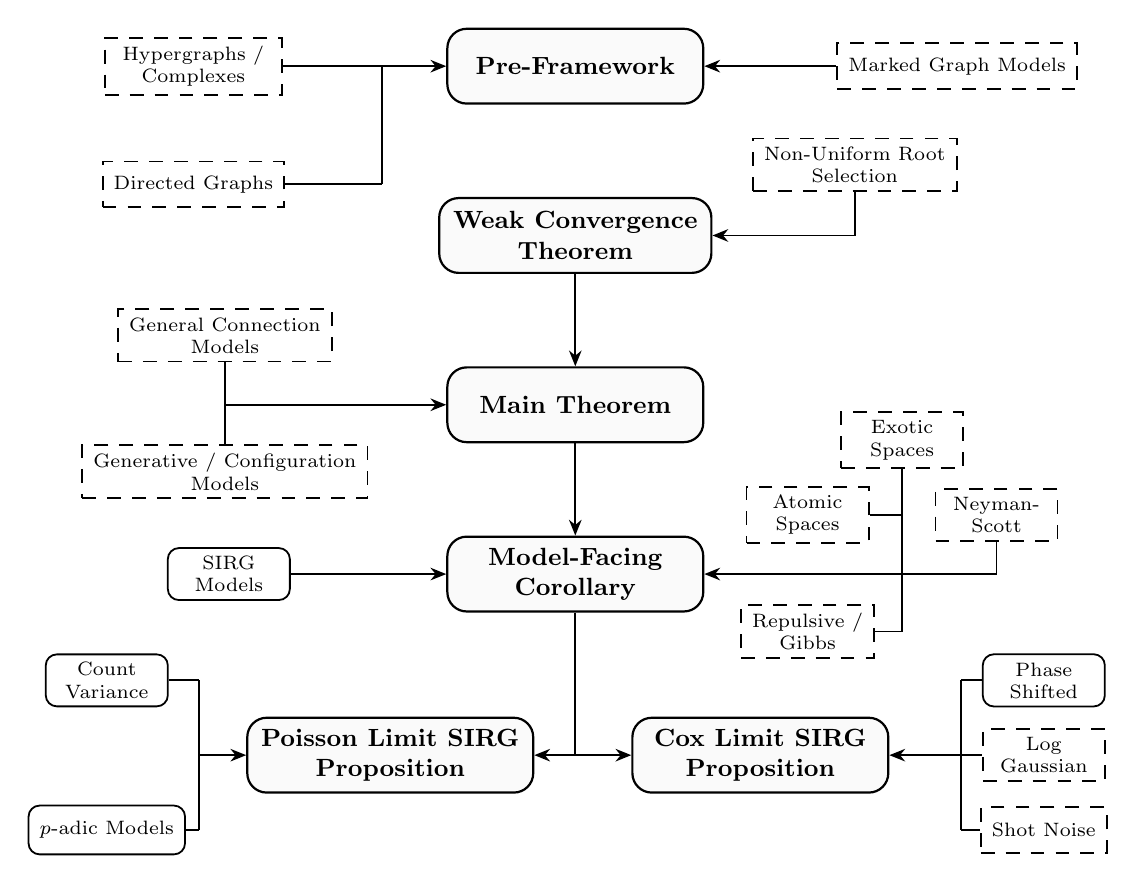
\begin{tikzpicture}[
  x=1cm,
  y=1cm,
  every node/.style={align=center},
  mainbox/.style={
    draw,
    rounded corners=7pt,
    line width=0.8pt,
    fill=gray!4,
    font=\small\bfseries,
    minimum width=3.25cm,
    minimum height=0.95cm,
    inner xsep=5pt,
    inner ysep=4pt
  },
  auxbox/.style={
    draw,
    dashed,
    dash pattern=on 5pt off 4pt,
    line width=0.65pt,
    font=\scriptsize,
    minimum width=2.25cm,
    minimum height=0.58cm,
    inner xsep=4pt,
    inner ysep=3pt
  },
  tinyaux/.style={
    auxbox,
    minimum width=1.55cm
  },
  solidaux/.style={
    draw,
    rounded corners=4pt,
    line width=0.65pt,
    font=\scriptsize,
    minimum width=1.55cm,
    minimum height=0.62cm,
    inner xsep=4pt,
    inner ysep=3pt
  },
  arrow/.style={-{Stealth[length=2.0mm,width=1.6mm]}, line width=0.65pt},
  wire/.style={line width=0.65pt}
]
  % Central result chain.
  \node[mainbox] (pre) at (0,0) {Pre-Framework};
  \node[mainbox] (weak) at (0,-2.15) {Weak Convergence\\Theorem};
  \node[mainbox] (local) at (0,-4.30) {Main Theorem};
  \node[mainbox] (sirg) at (0,-6.45) {Model-Facing\\Corollary};
  \node[mainbox] (poisson) at (-2.35,-8.75) {Poisson Limit SIRG\\Proposition};
  \node[mainbox] (cox) at (2.35,-8.75) {Cox Limit SIRG\\Proposition};

  \draw[arrow] (weak.south) -- (local.north);
  \draw[arrow] (local.south) -- (sirg.north);
  \draw[wire] (sirg.south) -- (0,-8.75);
  \draw[arrow] (0,-8.75) -- (poisson.east);
  \draw[arrow] (0,-8.75) -- (cox.west);

  % Inputs to the pre-framework.
  \node[auxbox] (hyper) at (-4.85,0) {Hypergraphs /\\Complexes};
  \node[auxbox] (directed) at (-4.85,-1.5) {Directed Graphs};
  \coordinate (preleftbus) at (-2.45,0);
  \draw[wire] (hyper.east) -- (preleftbus);
  \draw[wire] (directed.east) -- (-2.45,-1.5);
  \draw[wire] (-2.45,-1.5) -- (preleftbus);
  \draw[arrow] (preleftbus) -- (pre.west);

  \node[auxbox] (marked) at (4.85,0) {Marked Graph Models};
  \draw[arrow] (marked.west) -- (pre.east);

  % Rooting variants feeding the weak-convergence theorem.
  \node[auxbox, minimum width=2.35cm] (rootselect) at (3.55,-1.25) {Non-Uniform Root\\Selection};
  \draw[arrow] (rootselect.south) |- (weak.east);

  % Connection-model inputs to local weak convergence.
  \node[auxbox, minimum width=2.55cm] (general) at (-4.45,-3.42) {General Connection\\Models};
  \node[auxbox, minimum width=2.55cm] (dependent) at (-4.45,-5.15) {Generative / Configuration\\Models};
  \coordinate (localbus) at (-4.45,-4.30);
  \draw[wire] (general.south) -- (dependent.north);
  \draw[arrow] (localbus) -- (local.west);

  % SIRG model family and ambient-space examples.
  \node[solidaux] (sirgmodels) at (-4.40,-6.45) {SIRG\\Models};
  \draw[arrow] (sirgmodels.east) -- (sirg.west);

  \node[tinyaux] (exotic) at (4.15,-4.75) {Exotic\\Spaces};
  \node[tinyaux] (atomic) at (2.95,-5.70) {Atomic\\Spaces};
  \node[tinyaux] (neyman) at (5.35,-5.70) {Neyman-\\Scott};
  \node[tinyaux] (repulsive) at (2.95,-7.18) {Repulsive /\\Gibbs};
  \coordinate (sirgspacebus) at (4.15,-6.45);
  \draw[wire] (exotic.south) -- (sirgspacebus);
  \draw[wire] (atomic.east) -- (4.15,-5.70);
  \draw[wire] (neyman.south) |- (sirgspacebus);
  \draw[wire] (sirgspacebus) |- (repulsive.east);
  \draw[arrow] (sirgspacebus) -- (sirg.east);

  % Inputs to the Poisson-limit proposition.
  \node[solidaux] (countvariance) at (-5.95,-7.80) {Count\\Variance};
  \node[solidaux] (padicmodels) at (-5.95,-9.70) {$p$-adic Models};
  \coordinate (poissonbus) at (-4.78,-8.75);
  \draw[wire] (-4.78,-7.80) -- (-4.78,-9.70);
  \draw[wire] (countvariance.east) -- (-4.78,-7.80);
  \draw[wire] (padicmodels.east) -- (-4.78,-9.70);
  \draw[arrow] (poissonbus) -- (poisson.west);

  % Inputs to the Cox-limit proposition.
  \node[solidaux] (phaseshifted) at (5.95,-7.80) {Phase\\Shifted};
  \node[tinyaux] (loggaussian) at (5.95,-8.75) {Log\\Gaussian};
  \node[tinyaux] (shotnoise) at (5.95,-9.70) {Shot Noise};
  \coordinate (coxbus) at (4.90,-8.75);
  \draw[wire] (4.90,-7.80) -- (4.90,-9.70);
  \draw[wire] (phaseshifted.west) -- (4.90,-7.80);
  \draw[wire] (loggaussian.west) -- (4.90,-8.75);
  \draw[wire] (shotnoise.west) -- (4.90,-9.70);
  \draw[arrow] (coxbus) -- (cox.east);
\end{tikzpicture}

    \end{adjustbox}

    \vspace{0.3em}
    {\tiny
    Overview of the main convergence results and model families feeding into them.
    Dashed borders indicate topics not directly explored in this paper.
    }
\end{frame}

% --------------------------------------------------
\begin{frame}{Next Steps}
\begin{itemize}
    \item Preprint/Paper in the works with Pim van der Hoorn
    \item Directed graphs may be included in this revised framework
    \item Formalize conditions for more vertex processes (Cox, Neyman-Scott, ...)
    \item Hyperbolic SIRGs, eventually... 
\end{itemize}
\end{frame}

% --------------------------------------------------
\begin{frame}{Scan Me (Thesis, Related Notes, Notes on Presentation Slides)}
    \centering
    
\includegraphics[width=0.45\textwidth]{images/qrcode_400551511_83d8c8bd3467c58f9942d53733380a9b.jpg}
\end{frame}

\begin{frame}{The Pre-Main Theorem}
Consider a sequence of finite stationary adjacency processes $(\xi_n)_{n \in \mathbb{N}}$, placed along a $\text{nice}^*$ compact exhaustion of a proper metric space $\mathbb{X}^2$. Suppose that
\begin{enumerate}
    \item $\xi_n^{(o,o)} \Rightarrow \xi_\infty$ ($\xi_\infty$ will then also have a point at $(o,o)$ almost surely);
    \item The vertices concentrate via 
    $$\frac{|V(\xi_n)|}{\mathbb{E}|V(\xi_n)|}\overset{L^1}{\longrightarrow} 1;$$
    \item $(\xi_n^{(o,o)}, o)_{n \in \mathbb{N}}$ is \textit{radially} $\textit{tight}^*$ (vertices reachable from $o$ contained in a compact subset of $\mathbb{X}$ with high probability).
\end{enumerate}
Then, the corresponding graphs converge locally weakly, $$G(\xi_n, U_n) \Rightarrow G(\xi_\infty, o),$$ and $\xi_\infty$ acts as a nice, sampleable representation of the local weak limit. 
\end{frame}

\end{document}


